%\documentstyle[art10,titlepage,makeidx,twoside,EPSF/epsf,mytabbing]{j-article}

%%% added 2004.12.14
\documentclass[]{jarticle}
\usepackage{makeidx,mytabbing,fancyheadings}
\usepackage[dvipdfmx]{graphicx,color,epsfig}
\let\epsfile=\epsfig
\usepackage[dvipdfmx,bookmarks=true,bookmarksnumbered=true,bookmarkstype=toc]{hyperref}
\ifnum 42146=\euc"A4A2 \AtBeginDvi{\special{pdf:tounicode EUC-UCS2}}\else
\AtBeginDvi{\special{pdf:tounicode 90ms-RKSJ-UCS2}}\fi

%%%
\newcommand{\eusversion}{9.21}


\flushbottom
\makeindex
\pagestyle{myheadings}
\oddsidemargin=0cm
\evensidemargin=0cm

% A4 size
\textwidth=16.5cm
\textheight=24.6cm
\topmargin=-0.8cm
\oddsidemargin= 0.5cm
\evensidemargin=0.5cm

% Letter size
%\topmargin=0.5cm
%\textwidth=17.6cm
%\textheight=23cm
%\oddsidemargin= 0.2cm
%\evensidemargin=0.2cm

\parindent=10pt
\parskip=1mm
%\baselineskip 14pt

\setcounter{totalnumber}{3}
\renewcommand{\topfraction}{0.99}       % 85% of a page (from page
                                        % top)
                                        % can be occupied by tbl / fig
                                        %
\renewcommand{\bottomfraction}{0.99}    % 85% of a page (from page
                                        % bottom)
                                        % can be occupied by tbl / fig
\renewcommand{\textfraction}{0.0}      % text shoud occupy 15% or
                                        % more in
                                        % a page
%\renewcommand{\floatpagefraction}{0.99} % 70% or more shoud occupy in
                                        % a
                                        % a float page


%%% removed 2004.12.14 \jintercharskip=0pt plus3.0pt minus1pt%

\begin{document}

\newcommand{\ptext}[1]
{\tt \begin{quote} \begin{tabbing} #1 \end{tabbing} \end{quote} \rm}

\newcommand{\desclist}[1]{
\begin{list}{ }{\setlength{\rightmargin}{0mm}\topsep=0mm\partopsep=0mm}
\item #1
\end{list}
\vspace{3mm}}

\newcommand{\functiondescription}[4]{
\index{#1}
{\bf #1} \em #2 \rm \hfill [#3] 
%\if#4 \vspace{3mm} \\ \else \desclist{#4} \fi
%\ifx#4 \vspace{3mm} \\ \else \desclist{#4} \fi
 \desclist{\hspace{0mm}#4}
}

\newcommand{\bfx}[1]{\index{#1}{\bf #1}}
\newcommand{\emx}[1]{\index{#1}{\em #1}}

\newcommand{\longdescription}[3]{
\index{#1}
\begin{emtabbing}
{\bf #1} 
\it #2
\rm
\end{emtabbing}
\desclist{#3}
}

\newcommand{\funcdesc}[3]{\functiondescription{#1}{#2}{関数}{#3}}
\newcommand{\macrodesc}[3]{\functiondescription{#1}{#2}{マクロ}{#3}}
\newcommand{\specialdesc}[3]{\functiondescription{#1}{#2}{特殊}{#3}}
\newcommand{\methoddesc}[3]{\functiondescription{#1}{#2}{メソッド}{#3}}
\newcommand{\vardesc}[2]{\functiondescription{#1}{}{変数}{#2}}

\newcommand{\fundesc}[2]{\functiondescription{#1}{#2}{関数}{\hspace{0mm}}}
\newcommand{\macdesc}[2]{\functiondescription{#1}{#2}{マクロ}{\hspace{0mm}}}
\newcommand{\spedesc}[2]{\functiondescription{#1}{#2}{特殊}{\hspace{0mm}}}
\newcommand{\metdesc}[2]{\functiondescription{#1}{#2}{メソッド}{\hspace{0mm}}}

\newcommand{\constdesc}[2]{\functiondescription{#1}{}{定数}{#2}}

\newcommand{\classdesc}[4]{	%class, super slots description
\vspace{2mm} 
\index{#1}
{\Large {\bf #1 }} \hfill [クラス]  %super
\begin{tabbing}
\hspace{30mm} :super \hspace{5mm} \= {\bf #2} \\
\hspace{30mm} :slots \> #3 
\end{tabbing}
\vspace{4mm}
\desclist{#4}}

\newenvironment{refdesc}{
 \vspace{5mm} \parindent=0mm \topsep=0mm \parskip=0mm \leftmargin=10mm}{
             \parindent=10mm \topsep=3mm \parskip=1mm \leftmargin=0mm }


\date{}
\title{{\Huge \bf EusLisp} \\
{\large \bf version \eusversion} \\
{\LARGE \bf リファレンスマニュアル} \\
{\large -マルチスレッドとXToolKitの実現-} \\
\vspace{10mm}
%ETL-RM-87-06E \\
{\large ETL-TR-95-19} \\
{\large 1995年6月} \\ }

\author{
通商産業省 工業技術院 \\
電子技術総合研究所 知能システム部 \\
{\large 松井 俊浩, 原 功, 中垣 博文(九州電力)} \\
matsui@etl.go.jp, hara@etl.go.jp, nakagaki@etl.go.jp\\
〒305 茨城県つくば市梅園1-1-4 }

\thispagestyle{empty}
\maketitle
\pagenumbering{roman}
\tableofcontents
% \listoffigures
% \listoftables
\bibliographystyle{plain}
\newpage
\pagenumbering{arabic}
\part{EusLisp 基本}
\markboth{EusLisp version \eusversion リファレンスマニュアル (Part I)}{はじめに}
\section{はじめに}
\markright{\arabic{section}. はじめに}
EusLispは、知能ロボットの研究を目的とした言語で、Common Lispと
オブジェクト指向型プログラミングをベースとしている。ロボットの研究では、
センサデータの処理、環境認識、障害物回避動作計画、作業計画などが
重要なテーマとして取り上げられるが、これらに共通するのは、ロボットと
外界の3次元幾何モデルである。EusLispを開発する動機となったのは、
記号処理システムから簡単に使えて拡張性の高いソリッドモデラーの
必要性を痛感したからである。既存のソリッドモデラーを調べてわかったことは、
その実現にとって最も重要な機能は、数値演算ではなくモデル要素の
トポロジーを表現、管理するためのリスト処理能力であった。もちろん、
幾何演算も重要ではあるが、ベクトル・行列を操作する関数を組み込めば
十分であることがわかった。

こうして、ソリッドモデラーはLispの上に実現されるべきであると言う
基本方針が得られた。さらに、ソリッドモデラーは、3次元物体モデルを
定義し、動きをシミュレートし、物体の相互関係を表現し、グラフィックスを
表示する機能を提供するが、先に述べた各種のロボット問題と結合されなけ
れば意味がない。また、ロボットを完成されたシステムとして実現するには、
これらのロボット問題を解くモジュールが効果的に統合されなければならない。
EusLispは、この統合の枠組をオブジェクト指向に求めた。オブジェクト指向は、
モジュラープログラミングを促進し、継承機能により既存の機能を段階的に
拡張することが容易になる。実際、上記のソリッドモデラーは、物体、面、
エッジなどの物理的実体の振舞いをクラスに定義し、ロボット問題に依存する
機能は、これらをサブクラスに拡張することで効率よく発展させられる。
これは、ソフトウェア資源の再利用にもつながる。

こうしてEusLispは、オブジェクト指向とCommonLispをベースとして3次元幾何モデラー
を実現し、複数ロボットの協調動作に必要なタスク間通信機能、マンマシン
インタフェースに重要なウィンドウ、グラフィックス、複合的プログラミングに
必要な他言語インタフェース等を備え、さまざまなロボット問題への適用を
可能にしたプログラミングシステムとして構築された。このほか、メモリ管理にも
工夫を凝らし、メモリ容量以外に生じる領域の大きさに関する制約を極力
排除し、ガーベージコレクションが効率的に行なわれ、ユーザがメモリ管理に関する
パラメータを操作する必要がないように努めた。

このリファレンスマニュアルは、EusLispの基礎と拡張に分かれ、
前者がCommon Lispの機能とオブジェクト指向型プログラミングを、後者が
幾何モデル、ロボットモデル、ウィンドウ、画像処理など、よりロボット
応用に近い部分を扱っている。アップデート情報は、\ref{License}節に書かれ
ているとおり、Euslispのメーリングリストから入手することができる。

\subsection{EusLispにおけるオブジェクト指向プログラミング}
EusLisp は、その他のLispを基礎としたオブジェクト指向プログラム言語(
例えばCLOS \cite{CLOS:Keene})と異なり、オブジェクト指向を基礎とした
Lispシステムである。
以前の考え方として、Lispはオブジェクト指向プログラミングを実現するための
言語として使用され、その中でシステムのデータ型がそれ相応のクラスを
持っていなかったので、システム定義オブジェクトとユーザー定義
オブジェクトとの間に明らかな区別があった。
一方、EusLisp内の数値を除く全てのデータ構造は
オブジェクトで表現されている。
そして、内部データ型(例えば{\tt cons}や{\tt symbols})とユーザー定義クラス
との間に特別な違いはない。
これは、システムの内部データ型でさえユーザー定義のクラスによって
拡張(継承)できることを意味する。
また、ユーザーが内部クラスのサブクラスとして自分独自のクラスを定義したとき、
その新しいクラスに対して内部メソッドおよび内部関数を使用することができ、
新しいプログラムを記述する量を減らすことができる。
例えば、キューやtreeやスタックなどを定義するために、{\tt car}や{\tt cdr}
と異なった特別な部分を持つように{\tt cons}クラスを拡張したとする。
これらのインスタンスでさえ、
{\tt cons}クラスの内部関数が型の継承を一定時間で認識するため、
それらの関数をのロス時間なしで適用できる。
したがって、EusLispはシステムの全ての内部機能(拡張可能なデータ型の形式)を
プログラマーに公開している。
この画一性もまた、EusLispの実行のために役に立つ。なぜなら、実行言語の中で
{\bf defclass}や{\bf send}や{\bf instantiate}のような僅かな核になる関数を
定義した後は、内部データ型の内部構造にアクセスするための大部分の関数を
EusLisp自身で書くことができる。
これは、EusLispの確実性および維持性を改善するものである。

\subsection{Euslispの特徴}

\begin{description}
\item [オブジェクト指向プログラミング]
EusLispは、単一継承オブジェクト指向プログラミングである。
数値を除いた全てのデータ型は、オブジェクトで表現され、その動作は
それらのクラスの中に定義されている。
\item [Common Lisp] 
EusLispは、EusLispのゴールやオブジェクト指向と一致する限りにおいて、
\cite{CLtL}や\cite{CLtL2}に書かれているCommon Lispの文法に従う。
次の節に互換性について記述する。
\item [コンパイラ]
EusLispのコンパイラは、インタプリタによる実行よりも5〜30倍実行速度を
上げることができる。
コンパイラは、インタプリタと同一の構文を持っている。
\item[メモリ管理] 
フィボナッチバディ方法は、メモリ制御・GC・ロバスト制御に有効なため、
メモリ管理手法として、使用されている。
EusLisp は、比較的に平均的な量のメモリを持つシステムで動作できる。
ユーザーは、それぞれのデータ型毎のページアロケーションの最適化
を考える必要がない。
\item [幾何学関数]
数値は、いつも直接データとして表現されるため、
数値計算によってゴミは発生しない。
任意の大きさのベクトル・行列におけるたくさんの幾何学関数は、
内部関数となっている。
\item [幾何学モデラー]
立体モデルは、CSGの処理を使用して、基本的な形から定義することができる。
質量や干渉チェックや接触判別等を備えている。
\item [グラフィックス]
描画時の陰線処理やレンダリング時の陰面処理を備えている。
画像をポストスクリプトデータとして出力できる。
\item [画像処理]
エッジ抽出機能を備えている。
\item [マニピュレータモデル]
6自由度を持つロボットマニピュレータを簡単にモデル化できる。
\item [Xwindowインターフェース]
Xlibの関数呼び出しとXlibのクラスおよび独自のXToolKitクラスの3つの
レベルのXwindowインターフェースを備えている。
\item [他言語インターフェース]
Cや他の言語で書かれた関数をEusLispの中から呼び出すことができる。
EusLispと他言語間の両方向呼びだしを備えている。
LINPACKのようなライブラリ内の関数は、このインターフェースを通して実行される。
X toolkitのCall-back関数はLispへ定義することができる。
\item [UNIX依存関数]
ほとんどのUNIXのシステム呼びだしおよびライブラリ関数は、Lisp関数として
揃っている。
通信処理や非同期入出力も可能である。
\item[マルチスレッド]
グローバルデータを分割してマルチ処理を実現するマルチスレッドプログラミングが
Solaris 2オペレーティングシステムの上で可能となった。
マルチスレッドは、非同期プログラミングを容易にし、実時間応答を改善する\cite{MTEus1,MTEus2}。
もし、マルチプロセッサのマシン上でEuslispを実行するならば、並列プロセッサの
高い計算能力を利用することができる。
%\item[ディスク保存]
%EusLispの処理イメージは、初期ロードを容易にしかつ完全なアプリケーションを作るために
%ディスクファイルの中にセーブできる。
\end{description}

\subsection{Common Lispとの互換性}

Common Lispは、よく本となっていて広く入手できる標準的なLisp\cite{CLtL,CLtL2}
となっている。
そのため、EusLispはCommon Lispの特徴をたくさん採用している。例えば、
変数スコープルール・パッケージ・列・一般変数・ブロック・構造体・
キーワードパラメータなどであるが、非互換もまだ残っている。
実現されていない特徴を次に列挙する。

\begin{enumerate}
\item 多値変数:
      multiple-value-call, multiple-value-prog1, etc.
\item いくつかのデータ型:
      complex number, bignum, ratio, character, deftype
\item いくつかの特殊書式:
      progv, compiler-let,macrolet
\end{enumerate}

次の特徴は、まだ完全でない。:
\begin{enumerate}
\setcounter{enumi}{3}
\item  closure -- 動的範囲のみ有効である。
%\item  package --  no shadowing-list
\item  declare,proclaim -- inlineとignoreは認識されない。
\end{enumerate}

\subsection{開発履歴}
\begin{description}
\item[1986] EusLispの最初のバージョンがUNIX-System5/Ustation-E20上で走った。
フィボナッチバディのメモリ管理・M68020のアセンブラコードを生成するコンパイラ・
ベクトル/行列関数がテストされた。
\item[1987] 新しい高速型チェック方法が実現された。
他言語インタフェースとSunViewインターフェースが組み込まれた。
\item[1988] コンパイラは、中間コードとして、Cプログラムを生成するよう
変更された。
コンパイラが中央処理装置と無関係となったため、
EusLispは簡単にUltrix/VAX8800やSunOS3.5/Sun3や/Sun4の上に移植された。
ソケットを使用したIPC機能が追加された。
ソリッドモデラーが実現された。
Common Lispの特徴の大部分が追加された。例えば、キーワードパラメータ、
再帰的データオブジェクトを扱うための表示フォーマット、
一般列関数、
readtables, tagbody, go, flet, や labels special forms, 等。
\item[1989] Xlibインターフェースが作られた。
Cのような数式表現を読み込む\%マクロが作られた。
マニピュレータのクラスが定義された。
\item[1990] XViewインターフェースが稲葉氏により作成された。
レイトレーサが作成された。
ソリッドモデラーがCSG処理履歴を保持するよう修正された。
非同期入出力が追加された。
\item[1991] 動作拘束プログラムが比留川氏により作成された。
DEC stationに移植された。
Coordinatesクラスが2次元と3次元の両方の座標系を扱えるよう変更された。
Body組立関数が接触オブジェクトを扱えるよう拡張された。
接触オブジェクトのためのCSG処理が作られた。
パッケージシステムがCommon Lispと互換になった。
\item[1992]
2つの平面の結合や交差を求める{\bf face+}や{\bf face*}が追加された。
画像処理機能が追加された。
リファレンスマニュアルの第一版が発行され、配布された。
\item[1993]
Euslispは、全く変更がなかった。
\item[1994] Solaris 2に移植された。
Solarisのマルチスレッド機能を用いて、マルチタスクが実現された。
XToolKitが構築された。
マルチロボットシミュレータMARSが國吉氏により作成された。
福岡で開催された日本ロボット学会学術講演会において
Euslispのオーガナイズドセッションが開かれた。
\item[1995]
リファレンスマニュアルの第二版が発行された。
\item[2010] 修正BSDライセンスに変更され,バージョンが9.00となった.
\item[2011] Darwin OS サポートが追加された.モデルファイルが追加された.
\item[2013] Cygwin 64Bit サポートが追加された, MAXSTACK が 65536 から 8388608 へ、KEYWORDPARAMETERLIMIT が 32 から 128 に拡張された.
\item[2014] 文書がUTF-8 になった.バージョンが9.10となった.
\item[2015] min/maxのエラーチェック,vplus任意長対応, non-ttypモードでのメッセージ表示消去. バージョンが9.11となった.
\item[2015] ARMサポートが追加された.バージョンが9.12となった.
            class documentationが追加された.バージョンが9.13となった.
            assert 関数のAPIが変更された.message がオプションになった (defmacro assert (pred \&optional message).バージョンが9.14となった.
            文字比較関数の結果の誤りを修正した, /=関数で複数引数をサポートした, URLエンコード関数(escape-url)を追加した, interval-timeクラスの加減算でマイクロ秒をサポートした.バージョンが9.15となった.
            make-random-state関数が追加された, lib/llib/unittest.lのバグ修正.バージョンが9.16となった.
\item[2016] init-unit-testにtraceオプションを追加した.\#f(nan inf)をロードできるようにした.models/docの更新修正.バージョンが9.17となった.
            gcc-5対応を行った.バージョンが9.18となった.
\end{description}

\subsection{インストール}
インストールの手続きは、{\tt README}に記述されている。
インストールされるディレクトリ({\tt "/usr/local/eus/"}を仮定する)は、
グローバル変数{\tt *eusdir*}に設定される。この場所は、{\bf load}やコンパイラ
が参照する。

{\tt *eusdir*}のサブディレクトリは 、表\ref{Directories}に書いてあるとおり。
これらの中で、
{\tt c/, l/, comp/, geo/, clib/, lib/} や{\tt xwindow/}は、eusやeusxを作成するときの
基本ファイルを含んでいる。
その他は、付属ライブラリ・デモプログラム・ユーザーからの寄贈品である。

\begin{table}
\caption{\label{Directories}{\tt *eusdir*}のディレクトリ}
\begin{center}
{\footnotesize
\begin{tabular}{|l | l|}\hline 
FILES &  このドキュメント \\
README &  ライセンス・インストール・サンプル実行のガイド\\
VERSION &  EusLisp のバージョン\\
bin/ &  実行ファイル(eus, euscompとeusx)\\
c/ &  Cで書かれたEusLispのカーネル\\
l/ &  EusLispで書かれたカーネル関数\\
comp/ &  EusLispで書かれたEusLispコンパイラ\\
clib/ &  Cで書かれたライブラリ関数\\
doc/ &  ドキュメント(latexとjlatexのテキストとメモ)\\
geo/ &  幾何学関数とグラフィックプログラム\\
lib/ & 共有ライブラリ(.so)とスタートアップファイル\\
llib/ &  Lispライブラリ\\
llib2/ &  Lispライブラリ2(UTYOで開発)\\
xwindow/ &  X11インターフェース\\
makefile@ &  makefile.sun[34]os[34],.vax等へのシンボリックリンク\\
pprolog/ &  tiny prologのインタープリタ\\
xview/ &  xview tool kitインターフェース\\
tool/ & \\
vxworks/ & リアルタイムOS VxWorksとのインターフェース\\
robot/ & ロボットモデルとロボットシミュレータ(MARS)\\
vision/ &  画像処理プログラム\\
contact/ & 拘束動作解析 比留川氏作
\cite{Hirukawa:1991a,Hirukawa:1991b,Hirukawa:1991c}\\
demo/ &  デモプログラム\\
bench/ &  ベンチマークテスト用プログラム\\ \hline
\end{tabular}
}
\end{center}
\end{table}

\subsection{\label{License}ライセンス}
EusLispは以下の修正BSDライセンスの元配布されている.

\begin{verbatim}
Copyright (c) 1984-2001, National Institute of Advanced Industrial Science
All rights reserved.
ソースコード形式かバイナリ形式か、変更するかしないかを問わず、以下の条
件を満たす場合に限り、再頒布および使用が許可されます。

ソースコードを再頒布する場合、上記の著作権表示、本条件一覧、および下記
免責条項を含めること。
バイナリ形式で再頒布する場合、頒布物に付属のドキュメント等の資料に、上
記の著作権表示、本条件一覧、および下記免責条項を含めること。
書面による特別の許可なしに、本ソフトウェアから派生した製品の宣伝または
販売促進に、<組織>の名前またはコントリビューターの名前を使用してはなら
ない。
本ソフトウェアは、著作権者およびコントリビューターによって「現状のまま」
提供されており、明示黙示を問わず、商業的な使用可能性、および特定の目的
に対する適合性に関する暗黙の保証も含め、またそれに限定されない、いかな
る保証もありません。著作権者もコントリビューターも、事由のいかんを問わ
ず、 損害発生の原因いかんを問わず、かつ責任の根拠が契約であるか厳格責
任であるか(過失その他の)不法行為であるかを問わず、仮にそのような損害
が発生する可能性を知らされていたとしても、本ソフトウェアの使用によって
発生した(代替品または代用サービスの調達、使用の喪失、データの喪失、利
  益の喪失、業務の中断も含め、またそれに限定されない)直接損害、間接損
害、偶発的な損害、特別損害、懲罰的損害、または結果損害について、一切責
任を負わないものとします。
\end{verbatim}

なお8.25版までは以下のライセンスで配布されていた.

ユーザーは、メーリングリスト(euslisp@etl.go.jp)に登録され、そこにQ&A・バグ・
アップデート情報を流す。
この情報は、{\tt *eusdir*/doc/mails}に蓄積されている。

\begin{enumerate}
\item EusLispの著作権は作者(松井俊浩)および電子技術総合研究所に属する。
ユーザーは、作者より使用許可を得る必要がある。
\item 軍事目的以外であればどんな目的のためにEusLispを使用してもよい。
\item EusLispはftp経由で電子技術総合研究所から自由に得ることができる。
\item EusLispはここの条項を守る限りにおいてコピーまたは販売しても構わない。
ただし、販売する際、販売者はオリジナルのEusLispが無料であることを消費者に
通知しなければならない。
\item ライセンス取得者がEsuLispを使用して研究・学習した結果を公表する際、
EusLispの使用を特定参考文献として引用しなければならない。
\item ライセンス取得者は、EusLispのソースコードを追加・変更してもよい。
プログラム結果は、コードの50\%以上が変更されない限りEusLispであり、
変更していない部分については、これらの条項を守る必要がある。
\item EusLispで開発されたプログラムの著作権は、開発者に属する。
しかしながら、EusLisp本体の著作権に付け加えることはできない。
\item 作者および電総研は使用に際して、どんな保証もしない。
\end{enumerate}

\subsection{デモプログラム}
デモプログラムは、サブディレクトリ{\tt demo}の中にある。
{\tt *eusdir*}へ{\tt cd}した後、eusx上で実行できる。
\begin{description}
\item[ロボットアニメーション] \index{animation}
eusxより{\tt demo/animdemo.l}をロードする。
約20分の計算の後、ETA3マニピュレータの滑らかなアニメーションが表示される。
(図\ref{animdemo})
\item[レートレーシング] \index{ray-tracing}
もし、8ビットの疑似カラーディスプレイを持っているなら、
{\tt demo/renderdemo.l}をロードしてレイトレーシング画像を楽しむことができる。
{\tt geo/render.l}が先にコンパイルされていることが必要。
\item[エッジ抽出]
{\tt demo/edgedemo.l}をロードすると、サンプル単色画像が表示される。
微分オペレータとしきい値を選ぶためのパラメータを入力する。
エッジが数秒のうちに探され、元の画像に上書きされる。
\end{description}

\begin{figure}
\epsfile{file=fig/eta3colavo.ps,width=150mm}
\caption{\label{animdemo}衝突回避経路計画のアニメーション}
\end{figure}

\bibliography{/net/atom/usr/users/matsui/biblio/lang,/net/atom/usr/users/matsui/biblio/hirukawa}

\newpage



\section{データ型}
\markright{\arabic{section}. データ型}
他のLispと同様に、型の決まったデータオブジェクトは変数ではない。
どの変数もその値として、どんなオブジェクトも持つことができる。
変数にオブジェクトの型を宣言することが可能であるが、
一般的にコンパイラで高速なコードを生成するための情報としてのみ
使用される。
数値は、ポインタの中で直接値として表現され、
そのほかは、ポインタにより参照されるオブジェクトにより表現される。
Sun4で実行する場合、ポインタおよび数値は図\ref{Pointer}で描かれているように
long wordで表現される。
ポインタのLSBの2ビットは、ポインタ・integer・floatを識別するための
tagビットとして使用されている。
ポインタはtagビットが全てゼロであり、オブジェクトのアドレスとして32ビット全て
使用できるので、EusLispは4GB以上のアドレス空間を利用することができる。

\begin{figure}[hb]
\begin{center}
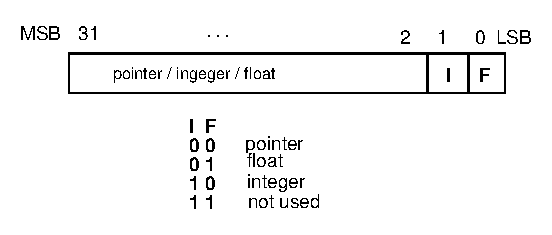
\includegraphics{fig/pointer.ps}
%\epsfile{file=fig/pointer.ps}
\end{center}
\caption{\label{Pointer}ポインタと直接値}
\end{figure}

\subsection{数値}
数値には、integerとfloat(浮動小数点)の2種類があり、
両方とも29ビットの値と1ビットの符号で表現される。
したがって、integerは$-$536,870,912から536,870,911までの範囲となる。
floatは、正および負で4.8E$-$38から3.8E38までの範囲を表現でき、
その有効数字は、十進数で約6桁すなわち浮動小数点誤差は1/1,000,000程度である。

数値は、いつもオブジェクトでなくポインタで表現される。
これは、EusLispのオブジェクト指向の唯一の例外事項である。
しかしながら、数値は決してヒープメモリを無駄にすることがないため、
数値を扱うアプリケーションでは、ガーベージコレクション
の原因とならず有効に動作する。

EusLispは、文字型を持たないため、文字列はintegerで表現される。
文字コード表と無関係なプログラムを書くためには、
%\#$\backslash$
\verb+#\+ 読みだしマクロが役に立つ。しかし、文字が読まれるとき、
数値表現に変換されるため、プリンタは
%\#$\backslash$
\verb+#\+ の表記法に対してどのように再変換すればよいのか解らない。

数値は、図\ref{Pointer}のlong wordの中に2つのtagビットを持っている。
それで、数値計算に使用するときは、シフトまたはマスクすることにより
このビットを消す必要がある。
integerは数値シフトによりMSBの2ビットを無視し、floatはマスクにより
LSBの2ビットを無視する。
VAXのようなアーキテクチャのためにByte swapも必要である。なぜなら、
意味を持つ最小の大きさのByteとして右端の1Byteが使用できないためである。


\subsection{オブジェクト}
数値でない全てのデータは、ヒープにおかれるオブジェクトで表現される。
それぞれのオブジェクトのメモリセルは、オブジェクトヘッダーと
オブジェクト変数のための固定数のスロットを持っている。
ベクトルは、任意の要素から構成されるため、
sizeスロットをヘッダーのすぐ後に持っている。
図\ref{ObjectFig}はオブジェクトとベクトルおよび
オブジェクトのヘッダーを描いたものである。
ここに示す{\em slot}と{\em element}のワードだけがユーザーから
アクセスすることができる。


\begin{figure}[hbt]
\begin{center}
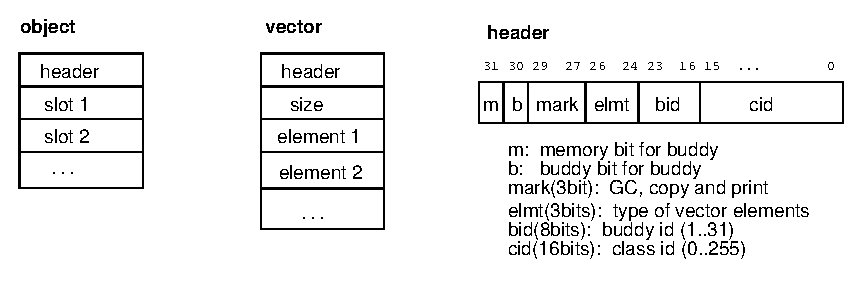
\includegraphics{fig/object.ps}
%\epsfile{file=fig/object.ps}
\end{center}
\caption{\label{ObjectFig}オブジェクト・ベクトル・オブジェクトヘッダーの構造}
\end{figure}

ヘッダーは、6つの部分で構成されている。
MSBの2ビット{\em m}と{\em b}は、フィボナッチバディメモリ管理手法の中で、
隣接セルの終端を示すために使用される。

{\em mark}部分には、3つのマークビットがあり、それぞれ
ガーベージコレクタ用のアクセス可能セルの認識、
プリンタ用の環状オブジェクトの認識(
{\tt \#n=}や{\tt \#n\#}表記法でプリントアウトさせた時)、
{\bf copy-object}用の分割オブジェクトのコピーとして使用される。
{\em elmt}部分は、ベクトル要素として使用可能な7つのデータ型(
{\tt pointer, bit, character, byte, integer, float, foreign-string})
のうち1つを識別するために使用される。
しかしながら、{\em elmt}はクラスの中で利用可能なため、
クラスの構造と無関係なメモリ管理ができ、
要素の高速なアクセスができる。
{\em bid}部分は、メモリセルの物理的大きさを表現する。
31の違った大きさ(16MB以上)のメモリセルをこの5ビットで表現する。
%with relatively finer resolution than the binary buddy method.
下位のshort word (16ビット)は、クラスID(cid)として使用される。
これは、システムのクラステーブルを経由してオブジェクトのクラスを
引き出すために使用される。
このクラスIDは、伝統的なLispの型tagとみなすことができる。
cidは下位8ビットのみが使用され、上位8ビットは無視される。
したがって、クラスの最大数は256が限界であるけれども、
システムのクラステーブルにもっとメモリを配置するように
EusLispを再構築することによって65536まで限界を引き上げることができる。

\subsection{クラス継承}

オブジェクトのデータ構造はクラスによって定義され、そして、それらの動作は
クラス内のメソッドに定義されている。
EusLispにおいて、数ダースのクラスが図\ref{ClassHierarchy}に書かれているように
木構造化された継承のなかにすでに定義されている。
{\bf class-hierarchy}関数を用いれば、実際の継承構造を見ることができる。
左端のクラスobjectは、EusLisp内の全てのクラスの根幹となるスーパークラスである。
ユーザーが定義したクラスは、これらの内部クラスのどれでも継承することができる。

\begin{figure}
\small
\begin{verbatim}
object
     cons
          queue
     propertied-object
          symbol   -----  foreign-pod
          package
          stream
               file-stream
               broadcast-stream
          io-stream ---- socket-stream
          metaclass
               vectorclass
                    cstructclass
          read-table
          array
          thread
          barrier-synch
          synch-memory-port
          coordinates
               cascaded-coords
                    body
                    sphere
                    viewing
                         projection
                              viewing2d
                              parallel-viewing
                              perspective-viewing
                    coordinates-axes
               viewport
          line --- edge --- winged-edge
          plane
               polygon
                    face
                    hole
               semi-space
          viewer
          viewsurface  ----- tektro-viewsurface
     compiled-code
          foreign-code
          closure
          load-module
     label-reference
     vector
          float-vector
          integer-vector
          string
               socket-address
               cstruct
          bit-vector
          foreign-string
     socket-port
     pathname
     hash-table
     surrounding-box
     stereo-viewing
\end{verbatim}
\normalsize
\caption{\label{ClassHierarchy}定義済みのクラス継承}
\end{figure}

クラスは、{\bf defclass}マクロか{\bf defstruct}マクロで定義される。

\ptext{
(defclass class-name \&key \= :super \hspace{15mm} \= class \\
 \> :slots \> () \\
 \> :metaclass \> metaclass \\
 \> :element-type \> t \\
 \> :size  -1\\ ) \\
(defstruct struct-name slots...) \\
(defstruct (struct-name [struct-options ...]) \\
\hspace{25mm}        (slot-name1 [slot-option...]) \\
\hspace{25mm}        (slot-name2 [slot-option...]) \\
\hspace{25mm}         ...) \\}

メソッドは、{\bf defmethod}により定義される。
{\bf defmethod}は、特定のクラスについて何度でも存在することができる。

\ptext{
(defmethod class-name  \\
 (:method-name1 (parameter...) . body1) \\
 (:method-name2 (parameter...) . body2) \\
 ...)
}

内部クラスにおけるfield定義は、大部分が
{\tt *eusdir*/c/eus.h}のヘッダーファイルの中にある。

{\em クラス}は、{\tt (describe)}関数によりクラス内の全てのスロット、
名前、スーパークラス、スロット名、スロット型、メソッドリスト、
などを表示することができる。
内部クラスの定義は次の通りである。
クラスobjectはスーパークラスを持たないため、このスーパークラスはNILである。

\ptext{
(defclass {\bf object} :super {\bf NIL} :slots ())
}

\ptext{
(defclass {\bf cons} :super {\bf object} :slots (car cdr))
}

\ptext{
(defclass {\bf propertied-object} :super {\bf object} \\
 \hspace{20mm} \=   :slots (plist)) \hspace{10mm} ;property list \\
}

\ptext{
(defclass {\bf symbol} :super {\bf propertied-object} \\
\hspace{20mm} :slots (\=value \hspace{15mm} \= ;specially bound value \\
 \>      vtype \>                ;const(0),var(1),special(2)  \\
 \>      function \>             ;global func def \\
 \>      pname               \>  ;print name string \\
 \>      homepkg)) \>            ;home package \\}

\ptext{
(defclass {\bf foreign-pod} :super {\bf symbol} \\
\hspace{20mm} :slots (\=podcode \hspace{15mm} \= ;entry code \\
 \>      paramtypes \>      ;type of arguments  \\
 \>      resulttype)) \\}


\ptext{
(defclass {\bf package} :super {\bf propertied-object} \\
\hspace{20mm} :slots (\= names \hspace{15mm} \= ;list of package name and nicknames\\
\>                   uses \>  ;spread use-package list \\
\>                   symvector \> ;hashed obvector \\
\>                   symcount \>  ;number of interned symbols \\
\>                   intsymvector \> ;hashed obvector of internal symbols \\
\>                   intsymcount \>  ;number of interned internal symbols \\
\>                   shadows \> ;shadowed symbols \\
\>                   used-by)) \>  ;packages using this package \\}

\ptext{
(defclass {\bf stream} :super {\bf propertied-object} \hspace{20mm} \\
\hspace{20mm} :slots (\= direction \hspace{3mm} \= ;:input or :output, nil if closed \\
  \>                   buffer  \>  ;buffer string \\
  \>                   count \> ;current character index \\
  \>                   tail)) \>  ;last character index \\
}

\ptext{
(defclass {\bf file-stream} :super {\bf stream} \\
\hspace{20mm} :slots (\= fd \hspace{10mm} \= ;file descriptor (integer)\\
 \>                    fname))\> ;file name str; qid for msgq \\
}

\ptext{
(defclass {\bf broadcast-stream} :super {\bf stream}\\
\hspace{20mm} :slots (destinations)) \hspace{10mm} ;streams to which output is e
livered}

\ptext{
(defclass {\bf io-stream} \= :super {\bf propertied-object}\\
\>        :slots (instream outstream))}

\ptext{
(defclass {\bf socket-stream} \= :super {\bf io-stream}\\
\>        :slots (address)) \hspace{20mm} ; socket address}

\ptext{
(defclass {\bf read-table}  :super {\bf propertied-object} \\
\hspace{20mm}      :slots (\= syntax \hspace{10mm} \= ; byte vector representing character types \\
\>\> ; 0:illegal, 1:white, 2:comment, 3:macro\\
\>\> ; 4:constituent, 5:single\_escape\\
\>\> ; 6:multi\_escape, 7:term\_macro, 8:nonterm\_macro \\
\> macro \> ;character macro expansion function\\
\> dispatch-macro)) \\}

\ptext{
(defclass {\bf array} :super {\bf propertied-object} \\
\hspace{20mm} :slots (\= entity \hspace{12mm}\= ;simple vector storing array entity \\
 \>           rank  \> ;number of dimensions: 0-7 \\
 \>           fillpointer \>    ;pointer to push next element \\
 \>           offset      \>    ;offset for displaced array \\
 \>           dim0,dim1,dim2,dim3,dim4,dim5,dim6))  ;dimensions \\}

\ptext{
(defclass {\bf metaclass} :super {\bf propertied-object} \\
\hspace{20mm}   :slots   (\= name  \hspace{8mm} \= ;class name symbol \\
 \>           super   \>   ;super class \\
 \>           cix  \>      ;class id \\
 \>           vars  \>     ;var name vector including inherited vars \\
 \>           types  \>    ;type vector of object variables \\
 \>           forwards \>  ;components to which messages are forwarded \\
 \>           methods))  \>  ;method list \\ }

\ptext{
(defclass {\bf vectorclass} :super {\bf metaclass}  \\
\hspace{20mm} :slots (\= element-type  \hspace{4mm} \= ;vector element type 0-7\\
 \>                 size)) \>  ;vector size; 0 if unspecified \\ }

\ptext{
(defclass {\bf cstructclass} :super {\bf vectorclass}  \\
\hspace{20mm} :slots (\= slotlist))  \hspace{4mm} \= ;cstruct slot descriptors\\}

\ptext{
(defclass {\bf vector} :super {\bf object} :slots (size))}

\ptext{
(defclass {\bf float-vector} :super {\bf vector} :element-type :float)}

\ptext{
(defclass {\bf string} :super {\bf vector} :element-type :char)}

\ptext{
(defclass {\bf hash-table} :super {\bf propertied-object} \\
\hspace{20mm}  :slots   (\= lisp::key \hspace{20mm}\= ;hashed key vector\\
\> value \> ; value vector\\
\> size \> ; the size of the hash table\\
\> count \> ; number of elements entered in the table\\
\> lisp::hash-function \> \\
\> lisp::test-function \\
\> lisp::rehash-size \\
\> lisp::empty  lisp::deleted )) \\
}

\ptext{
(defclass {\bf queue} :super {\bf cons})}

\ptext{
(defclass {\bf pathname} :super {\bf propertied-object} \\
\hspace{20mm}  :slots   (\= lisp::host device \hspace{20mm}\= ; not used\\
\> directory \> ; list of directories\\
\> name \> ; file name before the last "."\\
\> type \> ; type field after the last "."\\
\> lisp::version)) \> ; not used \\
}

\ptext{
(defclass {\bf label-reference} \hspace{8mm}  ;for reading \#n=, \#n\# objects \\
\hspace{20mm} \= :super {\bf object} \\
\>   :slots (label value unsolved next)) \\}

\ptext{
(defclass {\bf compiled-code} :super {\bf object} \\
\hspace{20mm}  :slots   (\= codevector \\
 \>          quotevector \\
 \>          type \hspace{15mm} \=    ;0=func, 1=macro, 2=special \\
 \>          entry))  \>  ;entry offset }

\ptext{
(defclass {\bf closure} \= :super {\bf compiled-code} \\
\>              :slots (env1 env2));environment}

\ptext{
(defclass {\bf foreign-code}  :super {\bf compiled-code}  \\
\hspace{20mm}  :slots   (\= paramtypes  \hspace{10mm} \=  ;list of parameter types\\
 \>              resulttype)) \> ;function result type}

\ptext{
(defclass {\bf load-module}  :super {\bf compiled-code}  \\
 \hspace{15mm}  :slots  (\= symbol-table \hspace{3mm} \= ;hashtable of symbols defined \\
 \>         object-file \> ;name of the object file loaded, needed for unloadin
\\
 \>         handle)) \> ;file handle returned by ''dlopen''}

\subsection{型指定}
Euslispは、{\bf deftype}特殊書式を持っていないけれども、
型名は宣言や結果あるいは中身の型の指定を要求する関数の中で
使用される。
例えば、{\bf coerce, map, concatenate, make-array}など。
一般に、クラス名は{\tt (concatenate cons "ab" "cd") = (97 98 99 100)}のように
型指定として使用することができる。このとき、Common Lispでは{\tt cons}の代わりに
{\tt (quote list)}を使用する。

Euslispは、数を表現するクラスを持っていないので、数の型はキーワードによって
与える必要がある。
{\bf :integer}, {\bf integer}, {\bf :int}, {\bf fixnum},
あるいは{\bf :fixnum}が整数型を表現するために使用され、
{\bf :float}あるいは{\bf float}が実数型を表現するために使用される。
{\bf make-array}の{\em element-type}引数においては、文字列を作るために
{\bf :character}, {\bf character}, {\bf :byte}や{\bfx byte}を
認識する。
{\bf defcstruct}, {\bf sys:peek}や{\bf sys:poke}のような低レベルの関数も、
バイト毎にアクセスするために
{\bf :character}, {\bf character}, {\bf :byte}あるいは{\bf byte}を認識し、
short word毎にアクセスするために
{\bf :short}あるいは{\bf short}を認識する。
どの場合においても、キーワードはpnameと同じ名前を持つlispパッケージのsymbol
を選ぶべきである。

\newpage

\section{書式と評価}
\markright{\arabic{section}. 書式と評価}
\subsection{アトム(atom)}

cons以外のデータオブジェクトは、たとえ複雑な構造をしていたとしても、
すべてatomである。
空リストとして()でしばしば書かれるNILもatomである。
すべてのatomは、symbolを除いていつもそれ自身評価されている。
しかしながら、他のCommon Lispの実行のなかでは、atomの評価に引用符を要求されることがある。

\subsection{スコープ}

すべてのsymbolは、値と結び付いている。
symbolは、主にくくられた文脈から決定される値によって評価される。
ここに2種類の変数バインドがある。それは、
ローカルまたは静的バインドとスペシャルまたは動的バインドである。
ローカルにバインドされた変数は{\bf lambda}書式または
{\bf let}や{\bf let*}の特殊書式においてspecialと宣言されない限り
外から見ることはできない。
ローカルバインドは入れ子が可能で、外側のローカルバインドやスペシャルバインドを隠して、
最も内側のレベルで定義されている1つのバインドのみ見ることができる。
スペシャル変数は2つの方法で使用される。
1つは、グローバル変数として、もう1つは動的に覗けるローカル変数として用いる。
このローカル変数は、バインドの効果の中にある限りローカルスコープの
外にいてさえ見ることができる。
後者の場合、スペシャル変数は{\bf special}で宣言される必要がある。
その宣言は、コンパイラだけでなくインタプリタでも認識される。
Common Lispによると、スペシャル変数は不明瞭なスコープと動的な
広さを持っていると言われている。

%\footnote{In Maclisp, all the variables are taken to be special by the
%interpreter, and lexical by the compiler if not declared special.
%In Etalisp, all variables are special and no declaration is recognized.}

あるスコープのなかで、ローカル変数が存在するとしても、
同じ変数名を内部スコープの中で{\bf special}として再宣言することができる。
{\bf symbol-value}関数は、ローカルスコープに構わずspecial値を引き出す
ために使用することができる。
{\bf set}関数は、スペシャル変数としてのみ働く。すなわち、
specialとして宣言していない限り、lambdaやlet変数の値を
変更するために使用することはできない。

\begin{verbatim}
(let ((x 1))
   (declare (special x))
   (let* ((x (+ x x)) (y x))
      (let* ((y (+ y y)) (z (+ x x)))
         (declare (special x))
         (format t "x=~S y=~s z=~s~%" x y z) ) ) )
--> x=1 y=4 z=2
\end{verbatim}

symbolは、{\bf defconstant}マクロにより定数として宣言することができる。
一旦宣言すると、その後値を変更しようとするとエラーが発生する。
そのうえ、そのような定数symbolは、ローカル変数としてさえ変数名として
使用されることを禁じられる。
NILやTは、そのような定数の例である。
keywordパッケージのsymbolは、いつも作成されるときに定数として宣言される。
対照的に、{\bf defvar}や{\bf defparameter}マクロは、スペシャル変数として
symbolを宣言する。
{\bf defvar}は、symbolがバインドされていない時のみ値の初期化を行い、
値が既に割り当てられているときは何もしない。
それに対して、{\bf defparameter}はいつも値をリセットする。

symbolが参照され、symbolのためのローカルバインドがなかったとき、
そのspecial値は、引き出される。
しかしながら、そのspecial値にまだ値が割り当ててなかったならば、
unbound variableエラーが発生する。

\subsection{一般化変数}
一般的に、どんな値および属性もオブジェクトのスロット(またはスタック)
で表現される。
スロットの値を引き出すかまたは変えるときは、
2つの基本的な命令、{\bf access}と{\bf update}で行わなければならない。
オブジェクトの全てのスロットに対して2つの異なった基本命令を定義する代りに
EusLispでは、Common Lispのように、一般化変数コンセプトに基づいた
画一的な更新命令を備えている。
このコンセプトのなかで、共通書式は、値のアクセス書式あるいはスロットの位置指定
として認識される。
したがって、それぞれのスロットに対してアクセスする書式を覚えてさえおけば、更新は
そのアクセス書式と{\bf setf}マクロを組み合わせることにより
実現できる。
例えば、car値をリストの外に取り出すのと同じ様に{\tt (setf (car '(a b)) 'c)}
として{\bf setf}を使用したとき、{\tt (car x)}は{\tt x}のcarスロットのなかの
値を置き換えることに使用することができる。

この方法は、ユーザーが定義したオブジェクト全てに対して
適用できる。
クラスや構造体が定義されるとき、それぞれのスロットに対する
accessやupdate書式は、自動的に定義される。
それらの書式は、それぞれマクロとして定義されている。その名前は、
クラス名とスロット名の連結となる。
例えば、consのcarは{\tt (cons-car '(a b c))}で処理することができる。

\begin{verbatim}
(defclass person :super object :slots (name age))
(defclass programmer :super person :slots (language machine))
(setq x (instantiate programmer))
(setf (programmer-name x) "MATSUI"
      (person-age x) 30)
(incf (programmer-age x))
(programmer-age x)   --> 31
(setf (programmer-language x) 'EUSLISP
      (programmer-machine x) 'SUN4)
\end{verbatim}

行列要素も同じ手法でアクセスすることができる。

\begin{verbatim}
(setq a (make-array '(3 3) :element-type :float))
(setf (aref a 0 0) 1.0 (aref a 1 1) 1.0 (aref a 2 2) 1.0)
a --> #2f((1.0 0.0 0.0) (0.0 1.0 0.0) (0.0 0.0 1.0))

(setq b (instantiate bit-vector 10))  --> #*0000000000
(setf (bit b 5) 1)
b --> #*0000010000
\end{verbatim}

特定のオブジェクトに特別なsetfメソッドを定義するために
{\bf defsetf}マクロを用意している。

\begin{verbatim}
(defsetf symbol-value set)
(defsetf get (sym prop) (val) `(putprop ,sym ,val ,prop))
\end{verbatim}

\subsection{特殊書式}

\begin{table}
\caption{\label{SpecialForms}EusLispの特殊書式}
\begin{center}
{\large
\begin{tabular}{|l l l|} \hline 
and & flet & quote \\
block & function & return-from\\
catch & go & setq \\
cond & if & tagbody \\
declare & labels & the \\
defmacro & let & throw \\
defmethod & let* & unwind-protect \\
defun & progn & while \\
eval-when & or & \\
\hline
\end{tabular} }
\end{center}
\end{table}

全ての特殊書式は、表\ref{SpecialForms}にリストされている。
{\bf macrolet, compiler-let,}や{\bf progv}は、該当しない。
特殊書式は、文脈の評価および制御フローの管理のための
基本的な言語構造である。
インタプリタとコンパイラは、これらの構造をそれぞれ正しく処理する
ために特殊な知識を持っている。それに対して、アプリケーションメソッド
は全ての関数に対し画一的である。
ユーザーは、独自の特殊書式定義を追加することはできない。

\subsection{マクロ}

マクロは、言語構造を拡張するために役立つメソッドである。
マクロが呼び出されたとき、引数は評価されずに
マクロの本体(マクロ拡張関数)へ受け渡される。
それから、マクロ拡張関数は、引数を拡張し、新しい書式を返す。
結果となった書式は、マクロの外側で再び評価される。
引数のリストにマクロまたは特殊書式を用いるとエラーになる。
{\bf macroexpand}関数は、マクロ展開のために使用することができる。

インタプリタのときマクロはゆっくりと実行されるが、
コンパイルすることにより実行速度の向上を図ることができる。
なぜなら、マクロ展開はコンパイル時に一度だけ行われ、
実行時にそのオーバーヘッドは残らない。
しかし、マクロ関数の中におけるevalあるいはapplyの呼出は、
インタプリタの実行とコンパイル後の実行との間に違う結果をもたらす。

\subsection{関数}

関数は、単にリストの最初の要素が{\bf lambda}であるようなlambda書式によって
表現される。
もしlambda書式が{\bf defun}を使ってsymbolを定義するとき、
グローバル関数名として参照することができる。
lambda書式は、次の文法で与えられる。

\ptext{
(lambda (\= \{var\}* \\
\>  [\&optional \{var $|$ (var [initform])\}*] \\
\>  [\&rest form] \\
\>  [\&key \= \{var $|$ (var [initform]) $|$ ((keyword var) [initform])\}* \\
\> \> [\&allow-other-keys]] \\
\>  [\&aux \{var $|$ (var [initform])\}*]) \\
 \hspace{10mm} \{declaration\}* \\
 \hspace{10mm} \{form\}*) \\
}

ここにEXPR,LEXPR,FEXPRなどのような型の関数はない。
関数への引数は、いつもその関数を実行する前に評価される。
受ける引数の数は、lambda-listによって決定される。
lambda-listは、lambda書式のためにパラメータの列を記す。

{\bf \&optional, \&rest, \&key }や{\bf \&aux} はそれぞれ、lambda-list
のなかに特殊な意味を持っていて、これらのsymbolは、変数名として使用
することはできない。
\&optionalや\&keyパラメータのsupplied-p変数は、サポートされていない。

lambda書式は、普通のリストデータと区別できないため、
{\bf function}特殊書式を用いて、インタプリタやコンパイラに関数として
認識するように知らせなければならない。
\footnote{CLtL-2のなかで、引用式lambda書式は、もはや関数でない。
そのような書式の適用はエラーとなる。}
{\bf function}は、関数の上に環境を固定するために重要である。
そのため、すべてのローカル変数はその関数が違ったローカルスコープの他の関数を
通ってきたとしてさえ、アクセスすることができる。
次のプログラムは、{\tt let}の{\tt sum}がlambda書式の中に見えるため、
インタプリタとコンパイル後のどちらも何もしない。


\begin{verbatim}
(let ((x '(1 2 3)) (sum 0))
  (mapc '(lambda (x) (setq sum (+ sum x))) x))
\end{verbatim}

予想した結果が得られるためには、次のように書くべきである。
\begin{verbatim}
(let ((x '(1 2 3)) (sum 0))
   (mapc #'(lambda (x) (setq sum (+ sum x))) x ))
\end{verbatim}

\#'は、{\bf function}の略語である。
すなわち、{\tt \#'(lambda (x) x)}は
{\tt (function (lambda (x) x))}と同等である。
ここは、funarg問題と呼ばれる別の例を示す。

\begin{verbatim}
(defun mapvector (f v)
    (do ((i 0 (1+ i)))
       ((>= i (length v)))
       (funcall f (aref v i))))
(defun vector-sum (v)
    (let ((i 0))
       (mapvector #'(lambda (x) (setq i (+ i x))) v)
       i))
(vector-sum #(1 2 3 4)) --> 10 
\end{verbatim}

EusLispのclosureは、不定な大きさを持つことができない。
すなわち、closureはその外側の大きさで可能な大きさまで持つことができる。
これはclosureが'generators'のプログラミングのために使用されないことを意味する。
次のプログラムは何もしない。

\begin{verbatim}
(proclaim '(special gen))
(let ((index 0))
   (setq gen #'(lambda () (setq index (1+ index)))))
(funcall gen)
\end{verbatim}

しかしながら、その同じ目的がオブジェクト指向プログラミングで実現できる。
なぜなら、オブジェクトはそれ自身の固定変数を持つことができるためである。
\begin{verbatim}
(defclass generator object (index))
(defmethod generator
 (:next () (setq index (1+ index)))
 (:init (&optional (start 0)) (setq index start) self))
(defvar gen (instance generator :init 0))
(send gen :next)
\end{verbatim}
\newpage

\section{制御構造}
\markright{\arabic{section}. 制御構造}
\subsection{条件文}

{\bf and,or}および{\bf cond}は、Common Lispにおいてマクロとして知られているが、
EusLispではインタプリタ時の効率を改善するために特殊書式として実行される。

\begin{refdesc}
\specialdesc{and}{\{form\}*}{
{\em form}は、NILが現れるまで左から右に評価される。
もし、全ての書式がnon-NILとして評価されるならば、
最後の値が返される。}

\specialdesc{or}{\{form\}*}{
{\em form}は、non-NIL値が現れるまで左から右に評価される。
そして、その値が返される。
もし、全ての書式がNILとして評価されるならば、NILを返す。}

\specialdesc{if}{test then [else]}{
{\bf if}は、1つの{\it then}と{\it else}書式のみを持つことができる。
そこに多重書式を書きたいときは、{\bf progn}を使って
グループ化しなければならない。}

\macrodesc{when}{test forms}{
{\bf if}と違って、
{\bf when}と{\bf unless}は、多重{\em 書式}で書くことを許可している。
{\em test}の評価がnon-NILのとき、{\bf when}は実行され、
評価がNILのとき、{\em unless}は実行される。
もう一方で、これらのマクロは{\em else}書式を追加することを
許可していない。}

\macrodesc{unless}{test forms}{
{\tt(when (not {\em test}) . {\em forms})}と同等である。}

\specialdesc{cond}{{(test \{form\}*)}*}{
任意の数の条件項は、{\bf cond}の後に続けることができる。
それぞれの条件項において、最初の書式{\em test}が評価される。
もし、non-NILであったとき、その条件項の残りの書式は、続いて評価される。
そして、最後の値が返される。
もし、{\em test}のあとに書式がなかったならば、
{\em test}の値が返される。
{\em test}が失敗したとき、次の条件項は{\em test}がnon-NIL評価されるかまたは
全ての条件項が尽きてしまうまで繰り返される。
条件項が尽きてしまった場合、{\bf cond}はNILを返す。}

\macrodesc{case}{key \{(\{label $|$ (\{lab\}*) \{form\}*)\}*}{
{\em key}と{\em label}が一致した条件項について、
{\em form}が評価され、最後の値が返される。
{\em key}と{\em label}の間の等価は、{\bf eq}または
{\bf memq}で行われ、{\bf equal}ではない。}

\end{refdesc}

\subsection{逐次実行とLet}

\begin{refdesc}
\funcdesc{prog1}{form1 \&rest forms}{
{\em form1}と{\em forms}は、次々と評価され、
{\em form1}から返される値が{\bf prog1}の値として返される。}

\specialdesc{progn}{\{form\}*}{
{\em form}は次々に評価され、最後の{\em form}の値が返される。
{\bf progn}は特殊書式である。なぜなら、ファイルの最初に現れたとき
特別な意味を持つからである。
そのような書式がコンパイルされたとき、内部書式はすべて最初に現れた
として見なす。
マクロが{\bf defun}や{\bf defmethod}の連続で拡張される場合、それが最初に
現われなければならないときに役立つ。}

\macrodesc{setf}{\{access-form value\}*}{
{\em value}を一般化変数{\em access-form}に割り当てる。}

\specialdesc{let}{(\{var $|$ (var [value])\}*) \{declare\}* \{form\}*}{
ローカル変数を生成する。
すべての{\em value}は評価され、並行して{\em var}に割り当てられる。すなわち、
{\tt (let ((a 1)) (let ((a (1+ a)) (b a)) (list a b)))} の結果は
(2 1)である。}

\specialdesc{let*}{(\{var $|$ (var [value])\}*) \{declare\}* \{form\}*}{
ローカル変数を生成する。
全ての{\em value}は次々に評価され、{\em var}に割り当てられる。すなわち、
{\tt (let ((a 1)) (let* ((a (1+ a)) (b a)) (list a b)))}の結果は
(2 2)である。}
\end{refdesc}

\subsection{ローカル関数}
\begin{refdesc}
\specialdesc{flet}{ (\{(fname lambda-list . body)\}*) \{form\}*}{
ローカル関数を定義する。}

\specialdesc{labels}{ (\{(fname lambda-list . body)\}*) \{form\}*}{
ローカルなスコープとなる関数を定義する。
{\bf flet}と{\bf labels}との違いは、
{\bf flet}で定義されたローカル関数は、その他の関数を参照または再帰できないが、
{\bf labels}は相互の参照を許可する。}
\end{refdesc}

\subsection{ブロックとExit}
\begin{refdesc}
\specialdesc{block}{tag \{form\}*}{
{\bf return-from}によって脱出可能なローカルブロックを作る。
{\em tag}は、ローカルにスコープされ、評価されない。}

\specialdesc{return-from}{tag value}{
{\em tag}によって示されたブロックを脱出する。
{\bf return-from}は、関数やメソッドから脱出するときに使用される。
関数やメソッドは、その本体をすべて取り囲んだ部分をブロックとして
自動的に確定され、その関数またはメソッドの名前を付ける。}

\macrodesc{return}{value}{
{\tt  (return x)}は、{\tt (return-from nil x)}と同等である。
{\bf loop, while, do, dolist, dotimes}は、暗黙的にNILと名前が付けられた
ブロックとして確定されるため、これらの特殊書式と組み合わせて使用する。}

\specialdesc{catch}{ tag \{form\}*}{
{\bf throw}によって脱出または値を返すための動的なブロックを確定する。
{\em tag}は評価される。

全て見える{\bf catch}の{\em tag}は、{\tt sys:list-all-catchers}から得ることができる。}

\specialdesc{throw}{tag value}{
{\bf catch}ブロックから脱出または{\em value}を返す。
{\em tag}と{\em value}は評価される。}

\specialdesc{unwind-protect}{protected-form \{cleanup-form\}*}{
{\em protected-form}の評価が終った後、
{\em cleanup-form}が評価される。
{\bf unwind-protect}の外側にブロックまたは{\bf catch}
ブロックを作っても構わない。

{\bf return-from}や{\bf throw}でさえ、そのようなブロックから
抜け出すためには{\em protected-form}の中で実行される。
{\em cleanup-form}は、評価されることが保証されている。
また、もし{\em protected-form}が実行されている間にエラーが起こったならば、
{\em cleanup-form}はいつも{\bf reset}によって実行される。}

\end{refdesc}

\subsection{繰返し}

\begin{refdesc}

\specialdesc{while}{test \{form\}*}{
{\em test}がnon-NILと評価されている間、
{\em form}は、繰返し評価される。
{\bf while}は、{\em form}のまわりにNILと名付けられるブロックを自動的に確定する
特殊書式である。
{\bf return}は、そのループから抜け出すために使用することができる。
次のイテレーションへ飛ぶときためには後に紹介する{\bf tagbody}と{\bf go}を次のように使う:}

\begin{verbatim}
(setq cnt 0)
(while
  (< cnt 10)
  (tagbody while-top
    (incf cnt)
    (when (eq (mod cnt 3) 0)
      (go while-top))  ;; jump to next iteraction
    (print cnt)
    )) ;; 1, 2, 4, 5, 7, 8, 10
\end{verbatim}

\specialdesc{tagbody}{\{tag $|$ statement\}*}{
{\em tag}は、{\bf go}のために名付けられる。
{\bf tagbody}の中のみ{\bf go}を使用することができる。}

\specialdesc{go}{tag}{
ローカルにスコープされた{\bf tagbody}のなかに現れる{\em tag}の直後の
書式に制御を移す。
ローカルスコープを横切って違う{\bf tagbody}のtagに制御を移すことは
禁止されている。}

\macrodesc{prog}{(\{var $|$ (var [init])\}*) \{tag $|$ statement\}*}{
{\bf prog}はマクロで、以下のように展開される。
\ptext{
(block nil 
    (let {\em var}
	(tagbody
		{\em tag $|$ statement})))}
}

\macrodesc{do}{(\{(var init [next])\}*) (endtest [result])\{declare\} \{form\}
*}
{{\em var}はローカル変数である。
それぞれの{\em var}に、{\em init}は並行に評価され、割り当てられる。
つぎに、{\em endtest}が評価され、もし真のとき{\bf do}は{\em result}を返す。
 (そうでないときは、NILを返す)
もし{\em endtest}がNILを返したならば、それぞれの{\em form}は、
順番に評価される。
書式の評価後、{\em next}が評価され、その値は
それぞれの{\em var}に再割当され、次の繰返しが始まる。}

\macrodesc{do*}{(\{var init [next]\}*) (endtest [result])\{declare\} \{form\}*}
{{\bf do*}は、{\em init}と{\em next}の評価と
{\em var}への割り当てが連続的に起こることを除いて、{\bf do}と同様である。}

\macrodesc{dotimes}{(var count [result]) \{forms\}*}{
{\em forms}の評価を{\em count}回行う。
{\em count}は、一回のみ評価される。
それぞれの評価の中で、{\em var}は整数のゼロから
{\em count}-1まで増加する。}

\macrodesc{dolist}{(var list [result]) \{forms\}*}{
{\em list}のそれぞれの要素は、{\em var}に連続的に与えられる。
そして{\em forms}は、それぞれの値で評価される。
{\bf dolist}は、他の繰返しより早く実行される。たとえば、
{\bf mapcar}や再帰的関数のようなものより。
それは、{\bf dolist}が関数のclosureを作ったり適用したりする必要が
なく、新しいパラメータのバインドが必要でないため。}

\macrodesc{until}{condition \{forms\}*}{
{\em condition}が満たされている間、{\em forms}を評価する。}

\macrodesc{loop}{\{forms\}*}{
{\em forms}を永遠に評価する。
実行を止めるためには、{\bf return-from, throw}または{\bf go}が
{\em forms}のなかで評価されなければならない。}

\subsection{述語}

Common Lispの{\bf typep}と{\bf subtypep}はないので、
{\bf subclassp}や{\bf derivedp}で疑似実現すること。

\begin{refdesc}

\funcdesc{eq}{obj1 obj2}{{\em obj1}と{\em obj2}が同じオブジェクトを指すポインタあるいは同じ
数値のときTを返す。
例えば:{\tt (eq 'a 'a)}はT、{\tt (eq 1 1)}はT、{\tt (eq 1. 1.0)}はNIL、
{\tt (eq "a" "a")}はNILである。}
\funcdesc{eql}{obj1 obj2}{
EusLispの中で数値は全て直接値で表現されるため、{\bf eq}と{\bf eql}は
同一である。}
\funcdesc{equal}{obj1 obj2}{
いろんな構造のオブジェクトの等価性をチェックする。オブジェクトは、文字列・ベクトル・
行列などで再帰的に参照してないことが保証されなければならない。
{\em obj1}や{\em obj2}が再帰的に参照されていたとすると、
{\bf equal}は無限ループとなる。}
\funcdesc{superequal}{obj1 obj2}{
{\bf superequal}は、環状参照をチェックするので遅い。しかしロバストな等価が得られる。}

\funcdesc{null}{object}{{\em object}がNILのとき、Tを返す。
{\tt (eq {\em object} nil)}を評価する。}
\funcdesc{not}{object}{
{\bf not}は、{\bf null}と同一である。}
\funcdesc{atom}{object}{
オブジェクトがconsのインスタンスである時のみ、NILを返す。
{\tt (atom nil) = (atom '()) = T)}\\
注意:vectors, strings, read-table, hash-tableなどに対しては、それらがどんなに
複雑なオブジェクトとなっていても{\bf atom}はTを返す。}
\funcdesc{every}{pred \&rest args}{
全ての{\em args}が{\em pred}についてTを返した時のみ
Tを返す。{\bf every}は、{\em pred}が全ての{\em args}に対して効力があるかどうかを
検査する時に使用される。}
\funcdesc{some}{pred \&rest args}{
{\em args}のうちどれか1つが{\em pred}についてTを返したとき
Tを返す。{\bf some}は、{\em pred}が{\em args}のどれかに対して効力があるかどうかを
検査する時に使用される。}
\end{refdesc}
\funcdesc{functionp}{object}{
{\em object}が{\bf apply}や{\bf funcall}で与えられる関数オブジェクトであるならTを返す。\\
注意:マクロは{\bf apply}や{\bf funcall}を適用することができない。
{\bf functionp}は、{\em object}が、type=0のコンパイルコードか、関数定義を持つsymbolか、
lambda-formかあるいはlambda-closureであったとき、Tを返す。
{\tt Examples: (functionp 'car) = T, (functionp 'do) = NIL}}
\funcdesc{compiled-function-p}{object}{
{\em object}が、コンパイルコードのインスタンスであったとき、Tを返す。
そのコンパイルコードが関数かまたはマクロかを知るためには、
そのオブジェクトに{\tt :type}メッセージを送り、その返り値が
{\tt function}と{\tt macro}のどちらになっているかを調べる。}

\end{refdesc}

\newpage

\section{オブジェクト指向プログラミング}
\markright{\arabic{section}. オブジェクト指向プログラミング}

オブジェクトの構造と動作は、クラスの中に記述されている。
それらは、{\bf defclass}マクロや{\bf defmethod}特殊書式により定義されている。
{\bf defclass}は、クラスの名前・そのスーパークラス・スロット変数名とオプションとして
任意の型およびメッセージの前方への送信を定義する。
{\bf defmethod}は、メッセージが送られてきたとき呼び出される
メソッドを定義する。
クラス定義は、symbolの特殊値として割り当てられる。
{\bf クラス}は、Common Lispの{\bf sutructure}のcounter部分と考えることができる。
スロットアクセス関数と{\bf setf}メソッドは、{\bf defclass}によってそれぞれの
スロットに自動的に定義される。

大部分のクラスは、内部クラス{\bf metaclass}から派生している。
{\bf metaclass}のサブクラスであるクラス{\bf vector-class}
はベクトルのためのメタクラスである。
もし、class-variablesやclass-methodsを使いたいときは、
{\bf metaclass}のサブクラスとして自分独自のメタクラスを作り、
メタクラスの名前を{\tt :metaclass}のキーワードで{\bf defclass}に与えればよい。

ベクトルは、その他のrecord-likeオブジェクトと違っている。
なぜなら、ベクトルのインスタンスは、任意の数の要素を持っているが、
record-likeオブジェクトは固定数のスロットを持っている。
EusLispのオブジェクトは、record-likeオブジェクトかまたはベクトルであって、
両方同時ではない。

要素の型が決められているかまたは要素が入れられないベクトルも
{\bf defclass}によって定義することができる。
次の例の中で、クラス{\tt intvec5}は5つのinteger要素を持つクラス
として定義されている。
自動型判定と型変換は、要素がインタープリタによってアクセスされたとき
実施される。
正しい宣言でコンパイルされたとき、高速なアクセスコードが生成される。

\begin{verbatim}
(defclass intvec5 :super vector :element-type :integer :size 5)
(setq x (instantiate intvec5))  --> #i(0 0 0 0 0)
\end{verbatim}

メッセージがオブジェクトに送られたとき、
一致するメッセージを最初そのオブジェクトのクラスから探し、次にそのスーパークラスから探して、
スーパークラスが尽きるまで探す。
もし、メソッドが定義されてなかったならば、
前方のリストが探される。
この前方探索は、疑似多重継承によって作られる。
もし、探索が失敗したときは、{\tt :nomethod}というメソッド名が探され、
メソッドは、全ての引数のリストと一緒に呼び出される。
次の例の中で、メッセージ{\tt :telephone}と{\tt :mail}は{\tt person}
という型のオブジェクトスロット{\tt secretary}に送られる。
そして、メッセージ{\tt go-home}はスロット{\tt chauffeur}に送られる。

\begin{verbatim}
(defclass president :super object
                    :slots ((name :type string)
                            (age  :type :integer)
                            (secretary  :type person
                                        :forward (:telephone :mail))
                            (chauffeur  :forward (:go-home))))
\end{verbatim}

メソッドにおいて、2つのローカル変数({\bf class}と{\bf self})
が使用可能となる。
これらの変数は変更すべきでない。
もし、変更したならば、システムから供給された変数は隠され、
{\bf send-super}と{\bf send self}は正しい動作をしない。


\subsection{クラスとメソッド}

\begin{refdesc}

\longdescription{defclass}
%{classname \&key \= :super object \hspace{85mm} [マクロ] \\
{classname \&key \= :super object \` [マクロ] \\
\> :slots (\{var $|$ (var [:type type] [:forward selectors])\}*) \\
\> :metaclass metaclass \\
\> :element-type t \\
\> :size -1\\}
{クラスを生成または再定義する。
異なったスーパークラスやスロットを持つクラスに再定義したとき、
メソッドが新しいスロット配置を仮定するため、
以前のクラスを継承する古いオブジェクトは予想できない振舞いをする。}

\specialdesc{defmethod}{classname \{(selector lambda-list . body)\}*}{
{\em classname}の1つ以上のメソッドを定義する。
それぞれの{\em selector}は、キーワードsymbolでなければならない。}

\macdesc{defclassmethod}{classname \{(selector lambda-list . body)\}*}

\funcdesc{classp}{object}{{\em object}がクラスオブジェクトのときTを返す。
そのオブジェクトは、クラス{\bf metaclass}かそのサブクラスの
インスタンスである。}

\funcdesc{subclassp}{class super}{
{\em class}が{\em super}のサブクラスであることを検査する。}

\funcdesc{vector-class-p}{x}{
{\em x}が、{\bf vector-class}のインスタンスであるとき、Tを返す。}

\funcdesc{delete-method}{class method-name}{
{\em method-name}のメソッド定義を{\em class}から除く。}

\funcdesc{class-hierarchy}{class}{
{\em class}の下の継承構造を表示する。}

\funcdesc{system:list-all-classes}{}{
今まで定義されたクラスを全てリストアップする。}

\funcdesc{system:find-method}{object selector}{
{\em selector}に記述されたメソッドを{\em object}のクラスおよび
そのスーパークラスの中から見つける。
{\em object}が、{\em selector}に応じることができるかどうかを
知るために使用される。}

\funcdesc{system:method-cache}{\&optional flag}{
メソッドキャッシュのヒット率を調査し、
ヒットとミスの2つの数値のリストを返す。
もし{\em flag}がNILのとき、メソッドキャッシュは無効になる。
もしnon-NILの{\em flag}が与えられたとき、メソッドキャッシュは初期化され
キャッシュ可能になる。}

\end{refdesc}

\subsection{メッセージ送信}
\begin{refdesc}

\funcdesc{send}{object selector \{arg\}*}{
{\em object}に{\em selector}と{\em arg}で構成されるメッセージを送信する。
{\em object}は、何でもよいが数値はいけない。
{\em selector}はキーワードとして評価されなければならない。}

\funcdesc{send-message}{target search selector \{arg\}*}{
{\bf send-super}を実行するための低レベル命令である。}

\macrodesc{send*}{object selector \&rest msg-list}{
{\bf send*}は、引数のリストに{\bf send-message}を適用する。
{\bf send}と{\bf send*}の関係は、
{\bf funcall}と{\bf apply}あるいは{\bf list}と{\bf list*}の関係に似ている。}

\funcdesc{send-all}{receivers selector \&rest mesg}{
全ての{\em receivers}に同じメッセージを送信し、結果をリストとして集める。}

\macrodesc{send-super}{selector \&rest msgs}{
{\em msgs}を{\tt self}に送信するが、
メソッドが定義されているクラスのスーパークラスでの
メソッドを探し始める。
メソッドの外の{\bf send-super}は、エラーとなる(すなわち、メソッド内で
なければならない)。}

\macrodesc{send-super*}{selector \&rest msg-list}{
{\bf send-super*}は、{\bf send-super}のapply版である。}

\end{refdesc}

\subsection{インスタンス管理}

\begin{refdesc}

\funcdesc{instantiate}{class \&optional size}{
{\em class}から新しいオブジェクトを作る低レベル命令である。
もし{\em class}が{\bf vector-class}ならば、{\em size}がなければならない。}

\macrodesc{instance}{class \&rest message}{
インスタンスが作られ、そこに{\em message}が送られる。}

\funcdesc{make-instance}{class \&rest var-val-pairs}{
{\em class}のインスタンスを作成し、スロット変数を
{\em var-val-pairs}のように設定する。
例えば、{\tt (make-instance cons :car 1 :cdr 2)}
は、{\tt (cons 1 2)}と同等である。}

\funcdesc{copy-object}{object}{
{\bf copy-object}関数は、参照トポロジー(再帰参照でも構わない)を保ったまま
コピーするために使用する。
{\bf copy-object}は、独自性の保存に触れないsymbolやパッケージを除いて、
{\em object}からアクセス可能などんなオブジェクトもコピーする。
{\bf copy-object}は、オブジェクトの中の全ての参照を2度妨害する。
1度が、新しいオブジェクトを作り既にコピーされたオブジェクトのオリジナルに
マークを付けるとき、そしてマークを消すときにもう1度。
この2段階の処理は、{\bf copy-object}を{\bf copy-seq}よりも遅くする。
もし順番にコピーをしたいならば、
{\bf copy-seq}か{\bf copy-tree}を使用することを薦める。}

\funcdesc{become}{object class}{
{\em object}のクラスを{\em class}に変更する。
古いクラスと新しいクラス両方のスロット構造は、一致しなければならない。
普通、2要素ベクトル間のクラス変更にのみ安全に使用することができる。
例えば、整数ベクトルからビットベクトルへの変更。}

\funcdesc{replace-object}{dest src}{
{\em dest}は、{\em src}のサブクラスのインスタンスでなければならない。}

\funcdesc{class}{object}{
{\em object}のクラスオブジェクトを返す。
クラス名を得るために、クラスオブジェクトに{\tt :name}メッセージを送る。}

\funcdesc{derivedp}{object class}{
{\bf derivedp}は、{\em object}が{\em class}またはそのサブクラスから
インスタンス化されているかどうかを判定する。
{\bf subclassp}と{\bf derivedp}関数は、クラス継承のなかを探索できない。
したがって、一定時間内に型のチェックがいつも終了する。}

\funcdesc{slot}{object class (index $|$ slot-name)}{
スロット値の名前かインデックスを返す。}

\funcdesc{setslot}{object class (index $|$ slot-name) value}{
{\bf setslot}は、内部処理関数でユーザーが使用できない。
代りに、{\bf setf}と{\bf slot}の組み合せを使用する。}

\end{refdesc}

\subsection{基本クラス}

\begin{refdesc}
\classdesc{object}{}
{}
{objectは、最も基本のクラスである。それは、クラス継承の最上位に位置する。
スロット変数が定義されていないため、{\bf object}はインスタンスを作るために
使用しない。}

\methoddesc{:prin1}{\&optional stream \&rest mesg}{
標準の再読み込可能なオブジェクトフォーマットのなかにあるオブジェクトを
表示する。
そのクラス名とアドレスは、角括弧でくくられ、符号を前に置く。
どのオブジェクトのサブクラスも{\em mesg}文字列で説明するマクロ{\bf send-super}
を使ってもっと広範囲な情報と一緒にそれ自身を印刷するのにこの方法を
使用することができる。
オブジェクトは、もし{\tt \#$<$}で始まるなら、再読み込み可能である。
%%% change 2004.12.14 そのクラス名・正確なアドレス・どのLispでも読み込可能な情報・\verb+>+をあとに
そのクラス名・正確なアドレス・どのLispでも読み込可能な情報・\verb~>~をあとに
従えて。
全てのデータオブジェクトは数値を除いて、{\bf object}を継承している。
この構文で書式の表示が得られる。(symbolや文字列でも構わない)
この構文で述べることは、symbolに{\bf setq}し忘れたデータオブジェクトを
把握することができる。
ただし、表示された後にガーベージコレクションが起こらない限りである。
}

\methoddesc{:slots}{}{
変数名のリストおよびオブジェクトの全てのスロットと対になる値を返す。
このリストに{\bf assoc}を適用することにより、スロットの詳細値が得られる。
しかしながら、それらを変更することはできない。}

\classdesc{propertied-object}{object}
{plist}
{property-listを持つオブジェクトを定義する。
他のCommon Lispと違って、
EusLispは、たとえ、symbolでなかったとしても、property-listを持つ
{\bf propertied-object}を継承するどんなオブジェクトも
許可する。}

\methoddesc{:plist}{\&optional plist}{
もし{\em plist}が明記されるならば、このオブジェクトの{\tt plist}スロットに
設定する。そのため、以前の{\tt plist}の値はなくなる。
{\em plist}は、
%%% change 2004.12.14 \verb+((indicator1 . value1) (indicator2 . value2) ...)+の書式にすべきである。
\verb~((indicator1 . value1) (indicator2 . value2) ...)~の書式にすべきである。
%%% change 2004.12.14 それぞれの\verb+indicator+は、{\bf eq}関数で等価
%%% 性をテストされたどのような
それぞれの\verb~indicator~は、{\bf eq}関数で等価性をテストされたどのような
lisp書式も可能である。
symbolが{\tt indicator}として用いられたとき、内部パッケージを広く実行される
等価性のチェックを確実にするためにキーワードの使用を推薦する。
{\bf :plist}は、主な{\tt plist}を返す。}
\methoddesc{:get}{indicator}{
{\tt plist}のなかで{\em indicator}と結び付く値を返す。
%%% change 2004.12.14 \verb+(send x :get :y) == (cdr (assoc :y (send x :plist)))+}
\verb~(send x :get :y) == (cdr (assoc :y (send x :plist)))~}
\methoddesc{:put}{indicator value}{
{\tt plist}のなかで、{\em value}と{\em indicator}を結び付ける。}
\methoddesc{:remprop}{indicator}{
{\tt plist}から{\em indicator}とvalueの組を削除する。
さらに、{\bf :get}を試すとvalueとしてNILを返す。}
\methoddesc{:name}{\&optional name}{
{\tt plist}のなかの{\tt :name}特性を定義し、取り出す。
この特性は、表示のために使用される。}
\methoddesc{:prin1}{\&optional stream \&rest mesg}{
再読み込み可能な書式のオブジェクトを表示する。
もしオブジェクトが{\tt :name}特性を持っているならば、
オブジェクトのアドレスの後に特性を表示する。}

\classdesc{metaclass}{propertied-object}
{name super cix vars types forwards methods}
{{\bf metaclass}は、複数クラスを定義する。独自のクラス変数を持つ複数クラスは、
それらのスーパークラスとして{\bf metaclass}を定義しなければならない。}
\methoddesc{:new}{}
{このクラスのインスタンスを生成し、全てのスロットをNILにした後、
それを返す。}
\methoddesc{:super}{}{
このクラスのスーパークラスオブジェクトを返す。
一旦クラス定義したスーパークラスを変更することはできない。}
\methoddesc{:methods}{}{
このクラスで定義された全てのメソッドのリストを返す。
そのリストは、メソッド名とパラメータと本体を組みにしたリスト
によって構成されたリストである。}
\methoddesc{:method}{name}{
{\em name}で関連づけられたメソッド定義を返す。
もし見つからなければ、NILを返す。}
\methoddesc{:method-names}{subname}{
メソッド名のなかに{\em subname}を含む全てのメソッド名のリストを返す。
メソッドは、このクラスのなかのみ探索される。}
\methoddesc{:all-methods}{}{
このクラスとその全てのスーパークラスのなかで定義されているすべてのメソッドの
リストを返す。
言い替えると、このクラスのインスタンスは、これらのメソッドを
実行することができる。}
\methoddesc{:all-method-names}{subname}{
{\em subname}と一致する全てのメソッド名のリストを返す。
その探索は、このクラスから{\bf object}まで実行される。}
\methoddesc{:slots}{}{
スロット名のベクトルを返す。}
\methoddesc{:name}{}{
このクラスのsymbol名を返す。}
\methoddesc{:cid}{}{
このクラスと同一であることを示すために、このクラスのインスタンスすべてに
割り当てられた整数を返す。
これは、システム内部のクラステーブルへのインデックスで、
このクラスの下に新しいサブクラスが定義されたとき、変更される。}
\methoddesc{:subclasses}{}{
このクラスの直接のサブクラスのリストを返す。}
\methoddesc{:hierarchy}{}{
このクラスの下に定義された全てのサブクラスのリストを返す。
全てのクラス継承の広範囲なリストを得るためには、{\bf class-hierarchy}関数
を呼び出す。}
\funcdesc{find-method}{object selector}{
{\em object}のクラスやそのスーパークラスのなかで、{\em selector}と一致する
メソッドを探索する。
この関数は、{\em object}のクラスが不確かで、その{\em object}が
エラーなしにメッセージを受け取ってくれるかどうかを知りたい時に役立つ。}
\end{refdesc}
\newpage

%\input{predicates}
\section{数値演算}
\markright{\arabic{section}. 数値演算}
\subsection{数値演算定数}
\begin{refdesc}
\constdesc{most-positive-fixnum}{\#x1fffffff=536,870,911。{\tt integer}の正の最大値。}
\constdesc{most-negative-fixnum}{-\#x20000000= -536,870,912。{\tt integer}の負の最大値}
\constdesc{short-float-epsilon}{IEEEの浮動小数点表現形式である{\tt float}は、
21ビットの固定小数(うち符号
が1ビット)と7ビットの指数(うち符号が1ビット)で構成されている。
したがって、浮動小数点誤差$\epsilon$は $2^{-21}= 4.768368 \times 10^{-7}$となる。}
\constdesc{single-float-epsilon}{{\bf short-float-epsilon}と同様に $2^{-21}$である。}
\constdesc{long-float-epsilon}{Euslispには、doubleもlong floatもないため、
{\bf short-float-epsilon}と同様に$2^{-21}$である。}
\constdesc{pi}{$\pi$。 実際には 3.14159203で、 3.14159265ではない。}
\constdesc{2pi}{$2\times \pi$。}
\constdesc{pi/2}{$\pi/2$。}
\constdesc{-pi}{-3.14159203。}
\constdesc{-2pi}{$-2\times \pi$。}
\constdesc{-pi/2}{$-\pi/2$。}
\end{refdesc}

\subsection{比較演算関数}
\begin{refdesc}
\funcdesc{numberp}{object}{
{\em object}が{\tt integer}か{\tt float}の時、Tを返す。
その文字が数字で構成されているときも同様である。}
\funcdesc{integerp}{object}{
{\em object}が{\tt integer}の時、Tを返す。
{\tt float}は{\bf round, trunc}および{\bf ceiling}関数で{\tt integer}に変換できる。}
\funcdesc{floatp}{object}{ {\em object} が {\tt float} の時 T を返す。
{\tt integer}は{\bf float}関数で{\tt float}に変換できる。}

\funcdesc{zerop}{number}{ {\em number}が{\tt integer}のゼロまたは
{\tt float}の0.0の時、 Tを返す。}
\funcdesc{plusp}{number}{{\em number}が正(ゼロは含まない)のとき、Tを返す。}
\funcdesc{minusp}{number}{{\em number}が負のとき、Tを返す。}

\funcdesc{oddp}{integer}{
{\em integer}が奇数のとき、Tを返す。引数は{\tt integer}のみ有効。}

\funcdesc{evenp}{integer}{
{\em integer}が偶数のとき、Tを返す。引数は{\tt integer}のみ有効。}

\funcdesc{/=}{num1 num2 \&rest more-numbers}{
{\em num1}と{\em num2}、{\em more-numbers}でどの2つの数値も等しくないとき、Tを返す。それ以外はNILを返す。
{\em num1}と{\em num2}、{\em more-numbers}を構成する要素はすべて数値であること。}

\funcdesc{=}{num1 num2 \&rest more-numbers}{
{\em num1}と{\em num2}、{\em more-numbers}がすべて等しいとき、Tを返す。
{\em num1}と{\em num2}、{\em more-numbers}を構成する要素はすべて数値であること。}

\funcdesc{$>$}{num1 num2 \&rest more-numbers}{
{\em num1}、{\em num2}、{\em more-numbers}の全要素がこの順に単調減少であるとき、Tを返す。
{\em num1}と{\em num2}、{\em more-numbers}を構成する要素はすべて数値であること。
誤差を含めた数値比較に対しては、
\ref{Geometry}章に書かれている関数({\bf eps$>$})を使用する。}

\funcdesc{$<$}{num1 num2 \&rest more-numbers}{
{\em num1}、{\em num2}、{\em more-numbers}の全要素がこの順に単調増加であるとき、Tを返す。
{\em num1}と{\em num2}、{\em more-numbers}を構成する要素はすべて数値であること。
誤差を含めた数値比較に対しては、
\ref{Geometry}章に書かれている関数({\bf eps$<$})を使用する。}

\funcdesc{$>=$}{num1 num2 \&rest more-numbers}{
{\em num1}、{\em num2}、{\em more-numbers}の全要素がこの順に単調非増加であるとき、Tを返す。
{\em num1}と{\em num2}、{\em more-numbers}を構成する要素はすべて数値であること。
誤差を含めた数値比較に対しては、
\ref{Geometry}章に書かれている関数({\bf eps$>=$})を使用する。}

\funcdesc{$<=$}{num1 num2 \&rest more-numbers}{
{\em num1}、{\em num2}、{\em more-numbers}の全要素がこの順に単調非減少であるとき、Tを返す。
{\em num1}と{\em num2}、{\em more-numbers}を構成する要素はすべて数値であること。
誤差を含めた数値比較に対しては、
\ref{Geometry}章に書かれている関数({\bf eps$<=$})を使用する。}
\end{refdesc}

\subsection{整数とビット毎の操作関数}
以下の関数の引数は、すべて{\tt integer}とする。

\begin{refdesc}
\funcdesc{mod}{dividend divisor}{
{\em dividend} を {\em divisor}で割った余りを返す。
{\tt (mod 6 5)=1, (mod -6 5)=-1, (mod 6 -5)=1, (mod -6 -5)=-1}.}

\funcdesc{1-}{integer}{
$integer-1$ を返す。コンパイラでは、引数を {\tt integer} と仮定する。}

\funcdesc{1+}{integer}{
$integer+1$ を返す。
{\bf 1+} と {\bf 1$-$} の引数は、{\tt integer} でなければならない。}
\funcdesc{logand}{\&rest integers}{{\em integers}のビット単位AND。}
\funcdesc{logior}{\&rest integers}{{\em integers}のビット単位OR。}
\funcdesc{logxor}{\&rest integers}{{\em integers}のビット単位XOR。}
\funcdesc{logeqv}{\&rest integers}{
{\bf logeqv}は{\tt (lognot (logxor ...))}と同等である。}
\funcdesc{lognand}{\&rest integers}{{\em integers}のビット単位NAND。}
\funcdesc{lognor}{\&rest integers}{{\em integers}のビット単位NOR。}
\funcdesc{lognot}{integer}{{\em integer}のビット反転。}
\funcdesc{logtest}{integer1 integer2}{
{\tt (logand {\em integer1 integer2})}がゼロでないとき T を返す。}

\funcdesc{logbitp}{index integer}{
{\em integer}がNILでなければ、LSBから数えて {\em index}番目の 
ビットが 1 のとき T を返す。}

\funcdesc{ash}{integer count}{
数値演算左シフト。
もし {\em count} が正のとき、{\em integer}を左にシフトする。
もし {\em count} が負のとき、
{\em integer} を $\vert${\em count}$\vert$ ビット右にシフトする。}

\funcdesc{ldb}{target position width}{
LoaD Byte.
{\bf ldb} や {\bf dpb} のByte型は、 EusLispにないため、代りに
2個の {\tt integer} を使用する。
{\em target} のLSBより{\em position}番目の位置からMSBへ {\em width} ビットの
範囲を抜き出す。例えば、 {\tt (ldb \#x1234 4 4)} は 3となる。}

\funcdesc{dpb}{value target position width}{
DePosit Byte.
{\em target}のLSBより{\em position}番目の位置へ{\em value}を
{\em width}ビット置き換える。}

\end{refdesc}


\subsection{一般数値関数}
\begin{refdesc}
\funcdesc{+}{\&rest numbers}{{\em numbers}の和を返す。}
\funcdesc{-}{num \&rest more-numbers}{
もし {\em more-numbers} が与えられたとき、{\em num}より引く。
そうでないとき、{\em num} は符号反転される。}
\funcdesc{*}{\&rest numbers}{{\em numbers}の積を返す。}
\funcdesc{/}{num1 num2 \&rest more-numbers}{
{\em num1} を、{\em num2} や {\em more-numbers}で割り算する。
全ての引数が{\tt integer}のとき、{\tt integer}を返し、
引数に1つでも{\tt float}があったときは、{\tt float}を返す。}
\funcdesc{abs}{number}{{\em number}の絶対値を返す。}
\funcdesc{round}{number}{
{\em number}の小数第1位を四捨五入し {\tt integer}を返す。
{\tt (round 1.5)=2, (round -1.5)=2}.}

\funcdesc{floor}{number}{
{\em number}の小数を切捨てる。
{\tt (floor 1.5)=1, (floor -1.5)=-2}.}

\funcdesc{ceiling}{number}{
{\em number}の小数を切り上げる。
{\tt (ceiling 1.5)=2, (ceiling -1.5)=-1}.}

\funcdesc{truncate}{number}{
{\em number}が正のときは切捨て、負のときは切り上げる。
{\tt (truncate 1.5)=1, (truncate -1.5)=-1}.}

\funcdesc{float}{number}{
 {\em number}を{\tt float}にして返す。}

\funcdesc{max}{\&rest numbers}{
 {\em numbers}の中から、最大値をさがす。}

\funcdesc{min}{\&rest numbers}{
{\em numbers}の中から、最小値をさがす。}

\funcdesc{random}{range \&optional (randstate *random-state*)}{
 0あるいは0.0 から {\em range}までの乱数を返す。
もし {\em range} が {\tt integer}のとき、
{\tt integer} に変換して返す。
そうでないとき、{\tt float} を返す。
オプションの{\em randstate} は、決まった乱数列で表される。
{\em randstate}に特別なデータの型はなく、
2つの要素からなる 整数ベクトルで表される。
}

\macrodesc{incf}{variable \&optional (increment 1)}{
{\em variable} は一般の変数である。
{\em variable} は、{\em increment}だけ増加され、
{\em variable}に戻される。}
\macrodesc{decf}{variable \&optional decrement}{
{\em variable} は一般の変数である。
{\em variable} は、{\em decrement}だけ減少され、
{\em variable}に戻される。}

\funcdesc{reduce}{func seq}{
2変数操作の{\em func}関数を用いて、{\em seq}の中の全ての要素を結合させる。
例えば、{\tt (reduce \#'expt '(2 3 4)) = (expt (expt 2 3) 4)=4096}.}

\funcdesc{rad2deg}{radian}{ラジアン値を 度数表現に変換する。
\#R は同じものである。
EusLisp の中での角度の表記はラジアンであり、
EusLisp 内の全ての関数が要求する角度引数は、ラジアン表現である。}

\funcdesc{deg2rad}{degree}{角度値をラジアン表現に変換する。
また \#D でも実行できる。}
\end{refdesc}

\subsection{基本関数}
\begin{refdesc}
\funcdesc{sin}{theta}{{\em theta} はラジアンで表される {\tt float} 値。
$\sin(theta)$を返す。}
\funcdesc{cos}{theta}{{\em theta} はラジアンで表される {\tt float} 値。
$\cos(theta)$を返す。}
\funcdesc{tan}{theta}{{\em theta} はラジアンで表される {\tt float} 値。
$\tan(theta)$を返す。}
\funcdesc{sinh}{x}{ hyperbolic sine、
$\frac{e^{x}-e^{-x}}{2}$で表される。}
\funcdesc{cosh}{x}{ hyperbolic cosine、
$\frac{e^{x}+e^{-x}}{2}$で表される。}
\funcdesc{tanh}{x}{ hyperbolic tangent、
$\frac{e^{x}+e^{-x}}{e^{x}-e^{-x}}$で表される。}
\funcdesc{asin}{number}{{\em number}のarc sineを返す。}
\funcdesc{acos}{number}{{\em number}のarc cosineを返す。}
\funcdesc{atan}{y \&optional x}{
{\bf atan} が1つの引数だけのとき、arctangent を計算する。
2つの引数のとき、{\tt atan}$(y/x)$ を計算する。}
\funcdesc{asinh}{x}{hyperbolic arc sine.}
\funcdesc{acosh}{x}{hyperbolic arc cosine.}
\funcdesc{atanh}{x}{hyperbolic arc tangent.}

\funcdesc{sqrt}{number}{{\em number} の平方根を返す。}

\funcdesc{log}{number}{{\em number} の自然対数を返す。}

\funcdesc{exp}{x}{$e^{x}$を返す。}

\funcdesc{expt}{a x}{
{\em a}の{\em x}乗を返す。}
\end{refdesc}

\newpage


\section{symbolとパッケージ}
\markright{\arabic{section}. Symbolとパッケージ}

\subsection{symbol}
symbolは、いつでも唯一であることが保証され、パッケージに収容される。
1つのパッケージのなかに、その他の
symbolとしておなじprint-nameを持っていることはあるが、symbol自体がコピーされることはない。
symbolがリーダに読まれるとき、symbolオブジェクトは、自動的に生成され、
1つのパッケージに収容される。
そのパッケージは、パッケージ名にコロン(:)を付け加えた接頭語によって
記すことができる。
そのようなパッケージ接頭語がないならば、symbolは{\bf lisp:*package*}
の値にある主なパッケージに収容される。
全てのsymbolは、1つのホームパッケージを持っている。
もしsymbolがそのようなホームパッケージを持っていないならば、
収容されていないsymbolと言われる。
収容されていないsymbolは、{\bf gensym}や{\bf make-symbol}関数によって
作ることができ、表示のときは、"{\tt \#:}"接頭語がつけられる。
これらのsymbolは収容されていないので、そのような2つのsymbolが同じ
print-nameを持っていた場合、等しいことが保証されない。

ふつう、lispリーダがsymbolに出会ったとき、リーダは自動的に
symbolのprint-name文字列を大文字に変換する。
したがって、例えば{\tt (symbol-name 'car)}と入力したとすると、
EusLispは、{\tt "car"}の代りに{\tt "CAR"}と答える。
{\tt (make-symbol "car")}は、{\tt car}や{\tt CAR}の代りに$|${\tt car}$|$
を返す。
もし、小文字から構成されるsymbolをリーダに作らせたい場合、
$\backslash$や$|...|$のようなエスケープを用いること。

\begin{refdesc}

\funcdesc{symbolp}{object}{ {\em object}が
クラスsymbolかそのサブクラスのインスタンスであったならば、Tを返す。}

\funcdesc{symbol-value}{symbol}{
{\em symbol}の特殊値を得る。ローカル変数値は、この関数では取り出す
ことはできない。}

\funcdesc{symbol-function}{symbol}{
{\em symbol}のグローバル関数定義を得る。
ローカル関数は、この関数で得られない。}

\funcdesc{symbol-package}{sym}{
{\em sym}が収容されているパッケージを返す。}

\funcdesc{symbol-name}{sym}{
{\em sym}のprint-nameを返す。
{\bf symbol-name}は、{\bf string}がコピーするのに反して、
 pname文字列をコピーしない。
したがって、もし{\bf symbol-name}で返された文字列を変えるならば
symbolは普通の内部手続きを通してアクセス不可能となる。}

\funcdesc{symbol-plist}{sym}{
{\em sym}のproperty-list(plist)を返す。
EusLispのplistは、関連リスト(association-list)と同じ様な書式を与える。
それは、属性名とその値の組を点でつないだ構成である。
これは、Common Lispの定義が要求するplist(属性名と値の線形リスト)
と非互換である。
EusLispにおいて、plistはsymbolに独特なものではない。
{\bf propertied-object}を継承するクラスから派生したどんなオブジェクトも、
property-listを持つことができる。
{\bf propertied-object}の中のこれらのplistを設定したり、取りだしたりするために、
{\bf propertied-object-plist}マクロは、{\bf symbol-plist}の代りに
使用されるべきである。
しかしながら、{\bf get}と{\bf putprop}はどのオブジェクトにも働く。}

\funcdesc{boundp}{symbol}{
{\em symbol}がグローバルな値を持っているかどうかを検査する。\\
注意:ローカル変数やオブジェクト変数として使用されるsymbolは
いつも値を持っているため、{\em boundp}はこれらのローカル変数の
格納状態を検査することができない。}
\funcdesc{fboundp}{symbol}{
{\em symbol}がグローバルな関数定義を持っているかどうかを検査する。}
\funcdesc{makunbound}{symbol}{
{\em symbol}は、(特殊値を持たないように)強制的にunboundされる。
ローカル変数は、いつも値が割り当てられ、{\bf makunbound}できない。}

\funcdesc{get}{sym attribute}{
{\em sym}のplistの中で{\em attribute}に関連する値を取り出す。
{\tt (cdr (assoc {\em attribute} (symbol-plist {\em sym})))}と等価である。}
\funcdesc{putprop}{sym val attribute}{
{\bf putprop}は、{\bf setf}と{\bf get}の組み合せで置き換えるべきである。}
\funcdesc{remprop}{sym attr}{
属性値({\em attr})と{\em sym}の組をproperty-listから削除する。}

\specialdesc{setq}{\{var value\}*}{
{\em value}を{\em var}に割り当てる。{\em var}は、symbolか点で継った組である。
{\em var}は、ローカル変数・オブジェクト変数・特殊変数の順番にその名前の中から探される。
ただし、明確にspecialと宣言されてないものに限る。}

\funcdesc{set}{sym val}{
{\em val}を{\em sym}の特殊値として割り当てる。
{\bf set}は、ローカル変数やオブジェクト変数に値を
割当てることはできない。}

\specialdesc{defun}{symbol [documentation] lambda-list . body}{
{\em symbol}にグローバル関数を定義する。
ローカル関数を定義するためには、{\bf flet}か{\bf labels}を使用すること。
もし、{\em documentation}が与えられない場合、lambda-listに書かれている
デフォルトのdocumentation文字列が入力される。}

\specialdesc{defmacro}{symbol [documentation] lambda-list . body}{
グローバルマクロを定義する。
EusLispは、ローカルスコープマクロ定義の機能を持っていない。}

\macrodesc{defvar}{var \&optional (init nil) doc}{
もし{\em var}が特殊値を持っていれば、{\bf defvar} は何もしない。
もし{\em var}がunboundならば、{\tt special}として宣言し、
{\em init}をその値として設定する。}

\macrodesc{defparameter}{var init \&optional doc}{
{\bf defparameter}は、{\em var}を{\tt special}として宣言し、
{\em var}が既に値を持っていたとしても、{\em init}をその値として設定する。}

\macrodesc{defconstant}{sym val \&optional doc}{
{\bf defconstant}は、{\bf val}を{\bf sym}の特殊値として設定する。
{\bf defvar, defparameter}や{\bf setq}と違い、その値は
{\bf defconstant}でのみ設定され、これらの書式で変更することができない。
もし定数symbolの値が、変更されようとしたならば、
エラーが返される。
しかし、{\bf defconstant}は以前の
定数値に上書きでき、上書きした場合は注意メッセージが出力される。}

\funcdesc{keywordp}{obj}{
もし{\em obj}がsymbolで、そのホームパッケージが{\bf KEYWORD}のときTを返す。}
\funcdesc{constantp}{symbol}{
もしsymbolが{\bf defconstant}マクロで定数に宣言されているときTを返す。}

\funcdesc{documentation}{sym \&optional type}{
{\em sym}のために提示文字列(documentation string)を取り出す。}

\funcdesc{gensym}{\&optional x}{
{\tt g001}のような前置文字列と付属数字を組み合わせた新しい収容されていないsymbolを作る。
収容されてないsymbolは、symbolに関連するパッケージがないため、パッケージ前置詞
の部分に\#:を示す。\#:が前につくsymbolは、読めないsymbolで、
リーダではこれらのsymbolへの参照を作成することができない。
{\em x}は、整数か文字列が可能で、
接頭(prefix)インデックスか接尾(suffix)値として使用される。}

\funcdesc{gentemp}{\&optional (prefix "T") (pkg *package*)}{
{\em pkg}に収容される新しいsymbolを作る。
ほとんどのアプリケーションにおいて、{\bf gensym}が{\bf gentemp}よりも好まれる。
なぜなら、収容されないsymbolの方が高速に作ることができ、
ガーベージコレクトも可能であるため。}

\end{refdesc}

\subsection{パッケージ}

パッケージは、symbolをグループ化するための区分された名前の付いた空間を与える。
複数のプログラマが要求されるような膨大なソフトウェアシステム
を開発しようとするとき、symbol(関数および変数名)が重複する問題を減少させるために
Common Lispでパッケージシステムが生まれた。
それぞれのパッケージは、内部symbolと外部symbolを持つ。
パッケージの中でsymbolが作成されたとき、いつでも内部symbolとなる。
{\bf export}を使用することにより外部symbolにすることができる。
異なったパッケージの外部symbolは、symbolの前にパッケージ名とコロン(:)を
つけることにより参照することができる。例えば、{\tt x:*display*}となる。
他のパッケージの内部symbolを参照する場合には、{\tt sys::free-threads}のように
ダブルコロン(::)を使用する。
前にパッケージ名をつけることを省略するためには、{\bf import}を用いる。
その上、{\bf use-package}を使用すれば、他のパッケージの全ての
外部symbolをimportすることができる。
symbolをexportあるいはimportするとき、あらゆるパッケージ内の
全てのsymbolが独自の
print-nameを持つ必要があるため、symbol名の重複を発見することができる。
{\bfx shadow}は、パッケージからsymbolを仮想的に削除することにより、
存在するsymbolと同じ名前のsymbolを作成することができる。

Euslispは次の8つのパッケージを定義する。
\begin{description}
\item [lisp:] 全てのlisp関数、マクロ、定数、など
\item [keyword:] キーワードsymbol
\item [unix:] UNIXシステムコールとライブラリ関数
\item [system:] システム管理または危険な関数; nicknames=sys,si
\item [compiler:] EusLispコンパイラ; nicknames=comp
\item [user:] ユーザー領域
\item [geometry:] 幾何学クラスとその関数
\item [xwindow:] X-windowインターフェース; nickname=x
\end{description}

これらのパッケージとユーザー定義パッケージは、システムの
package-listに繋げられている。
それは、{\bf list-all-packages}よって得ることができる。
それぞれのパッケージは、内部および外部symbolを探索・位置付けするために2つの
ハッシュテーブルを管理する。
また、パッケージは、その名前(stringまたはsymbol)とnick nameのリストと
そのパッケージが使う他のパッケージリストを記憶している。
{\bf *package*}は、読み込み・印刷のための主なパッケージを持つ
グローバル変数である。
もし{\bf *package*}が{\tt user:}でないならば、
top-levelプロンプトは、現在のパッケージを示すために{\tt mypkg:eus}\$のように変更される。

\begin{refdesc}
\constdesc{*lisp-package*}{ Lispパッケージ。}
\constdesc{*user-package*}{ ユーザーパッケージ。}
\constdesc{*unix-package*}{ UNIXパッケージ。}
\constdesc{*system-package*}{ システムパッケージ。}
\constdesc{*keyword-package*}{ キーワードパッケージ。}

\funcdesc{find-symbol}{string \&optional (package *package*)}{
{\em package}のなかでprint-nameとして{\em string}をもつsymbolを
見つける。
もし見つかったとき、そのsymbolが返され、そうでないときNILが返される。}

\funcdesc{make-symbol}{string}{
{\em string}で示される名前の新しい収容されていないsymbolを作る。}

\funcdesc{intern}{string \&optional (package *package*) (klass symbol)}{
{\em string}と同じprint-nameのsymbolを見つけようとする。
もし探索成功のとき、そのsymbolが返される。
もし失敗したとき、{\em string}というprint-nameを持つsymbolが新しく作られ、
{\em package}の中におかれる。}

\funcdesc{list-all-packages}{}{
今までに作られた全てのパッケージのリストを返す。}

\funcdesc{find-package}{name}{
パッケージの名前またはnicknameが{\em name}と同じものを探す。}
\funcdesc{make-package}{name \&key :nicknames (:use '(lisp))}{
{\em name}で示される名前の新しいパッケージを作る。
{\em name}は、stringあるいはsymbolでよい。
もしパッケージが既に存在している場合、エラーが報告される。}

\funcdesc{in-package}{pkg \&key :nicknames (:uses '(lisp))}{
現在のパッケージ({\bf *pacakge*}の値)を
{\em pkg}に変える。}

\funcdesc{package-name}{pkg}{
{\em pkg}パッケージの名前を文字列として返す。}

\funcdesc{package-nicknames}{pkg}{
{\em pkg}のnicknameのリストを返す。}

\funcdesc{rename-package}{pkg new-name \&optional new-nicknames}{
{\em pkg}の名前を{\em new-name}に変更し、そのnicknameを 
{\em new-nicknames}に変更する。
それらは、symbolかstringまたはsymbolかstringのリストのどれでも可能である。}

\funcdesc{package-use-list}{pkg}{
{\em pkg}で使用されるパッケージリストを返す。}

\funcdesc{packagep}{pkg}{
もし{\em pkg}がパッケージのときTを返す。}

\funcdesc{use-package}{pkg \&optional (curpkg *package*)}{
{\em pkg}を{\em curpkg}のuse-listに付け加える。
一旦追加すると、{\em pkg}のなかのsymbolは、パッケージの前置詞なしで
{\em curpkg}を見ることが可能になる。}

\funcdesc{unuse-package}{pkg \&optional (curpkg *package*)}{
{\em curpkg}のuse-listから{\em pkg}を削除する。}

\funcdesc{shadow}{sym \&optional(pkg *package*)}{
存在する{\em sym}を隠すことによって、
{\em pkg}内に内部symbolを作る。}

\funcdesc{export}{sym \&optional (pkg *package*)}{
{\em sym}は、symbolかsymbolのリストである。
{\bf export}は、{\em sym}を他のパッケージから
外部symbolとしてアクセス可能とする。
実際に、{\em sym}は、{\em pkg}のなかの外部symbolとして記録される。
もしsymbolが{\bf export}されると、パッケージマークとしてsingle colon ":"を使って
アクセス可能となる。これに対して、{\bf export}されていないsymbolはdouble colon "::"
で得られる。
そのうえ、{\bf export}されたsymbolは、
{\bf use-package}を使用したり、パッケージに{\bf import}されたとき、コロンの
必要がない。
symbolがexportされたかどうかは、それぞれのsymbolにでなくそれが収容されている
パッケージに属性付けられる。
それで、symbolは1つのパッケージの内部にあり、その他の外部となる。
{\bf export}は、{\em pkg}が使用している他のパッケージの中の
symbol名と{\em sym}が重複していないかどうかを検査する。
もし{\em sym}と同じprint nameをもつsymbolがあったならば、
"symbol conflict"とエラーを報告する。}

\funcdesc{unexport}{sym \&optional pkg}{
もし{\em sym}が{\em pkg}の外部symbolであったならば、unexportされ、
内部symbolとなる。}

\funcdesc{import}{sym \&optional (pkg *package*)}{
{\em sym}は、symbolまたはsymbolのリストである。
{\bf import}は、他のパッケージで定義されたsymbolを
{\em pkg}からパッケージの前置詞なしで内部symbolとして見えるようにする。
もし{\em sym}と同じprint-nameを持ったsymbolが既にあったとき、
"name conflict"とエラーを報告する。}

\macrodesc{do-symbols}{(var pkg) \&rest forms}{
{\em pkg}において、(内部あるいは外部)symbolに対して繰り返しをする。
そのときの{\em forms}の評価が返される。}

\macrodesc{do-external-symbols}{(var pkg) \&rest forms}{
{\em pkg}において、外部symbolに対して繰り返しをする。
そのときの{\em forms}の評価が返される。}


\macrodesc{do-all-symbols}{(var [result]) \&rest forms}{
全てのパッケージにおいて、symbolに対して繰り返しをする。そのときの{\em forms}の評価が返される。
もし、1つ以上のパッケージの中にそのsymbolが現れたならば、{\em forms}は、
1度以上評価される。}

\end{refdesc}

\newpage

\section{列、行列とテーブル}
\markright{\arabic{section}. 列、行列とテーブル}

\subsection{一般列}

ベクトル(1次元行列)とリストは、一般の列である。
文字列(string)は、文字(character)のベクトルなので、列である。

{\bf map, concatenate}や{\bf coerce}における結果の型を明記するためには、
クラスオブジェクトがsymbolにバインドされていないので、引用符なしで
{\tt cons, string, integer-vector, float-vector}などのクラス名symbolを使う。

\begin{refdesc}

\funcdesc{elt}{sequence pos}{
{\bf elt}は、{\em sequence}の中の{\em pos}番目の位置の値を得たり、({\bf setf}と
ともに)置いたりする最も一般的な関数である。
{\em sequence}は、リストまたは任意のオブジェクト、{\tt bit, char, integer, float}の
ベクトルである。
{\bf elt}は、多次元の行列に適用できない。}

\funcdesc{length}{sequence}{
{\em sequence}の長さを返す。
ベクトルにおいて、{\bf length}は一定の時間で終了する。
しかし、リスト型においては、長さに比例した時間がかかる。
{\bf length}が、もし環状リストに適用されたとき、決して終了しない。
代わりに{\bf list-length}を使用すること。
もし、{\em sequence}がfill-pointerを持つ行列ならば、
{\bf length}は行列全体のサイズを返すのではなくfill-pointerを返す。
このような行列のサイズを知りたい場合には、{\bf array-total-size}を
使用すること。
}

\funcdesc{subseq}{sequence start [end]}{
{\em sequence}の{\em start}番目から({\em end}$-$1)番目までをそっくりコピーした
列を作る。
{\em end}は、デフォルト値として{\em sequence}の長さをとる。}

\funcdesc{copy-seq}{sequence}{
{\em sequence}のコピーした列を作る。
このコピーでは、{\em sequence}のトップレベルの参照のみがコピーされる。
入れこリストのコピーには{\bf copy-tree}を使い、
再帰参照を持つような列のコピーには
{\bf copy-object}を使うこと。}

\funcdesc{reverse}{sequence}{
{\em sequence}の順番を逆にし、{\em sequence}と同じ型の新しい列を
返す。}

\funcdesc{nreverse}{sequence}{
{\bf nreverse}は、{\bf reverse}の破壊(destructive)バージョンである。
{\bf reverse}はメモリを確保するが、{\bf nreverse}はしない。}

\funcdesc{concatenate}{result-type \{sequence\}*}{
全ての{\em sequence}を連結させる。
それぞれの{\em sequence}は、なにかの列型である。
{\bf append}と違って、最後の一つまで含めた全ての列がコピーされる。
{\em result-type}は、{\tt cons,string,vector,float-vector}などの
クラスである。
}

\funcdesc{coerce}{sequence result-type}{
{\em sequence}の型を変更する。
例えば、{\tt (coerce '(a b c) vector) = \#(a b c)}や
{\tt (coerce "ABC" cons) = (a b c)}である。
{\em result-type}型の新しい列が作られ、
{\em sequence}のそれぞれの要素はその列にコピーされる。
{\em result-type}は、{\tt vector, integer-vector, float-vector, bit-vector, string, cons}
またはそれらの1つを継承したユーザー定義クラス
のうちの1つである。
{\bf coerce}は、{\em sequence}の型が{\em result-type}と同一である場合、コピーをする。}

\funcdesc{map}{result-type function seq \&rest more-seqs}{
{\em function}は、{\em seq}と{\em more-seqs}のそれぞれのN番目($N=0,1,\cdots$)の要素
からなるリストに
対して適用され、その結果は{\em result-type}の型の列に蓄積される。}

\funcdesc{fill}{sequence item \&key (:start 0) (:end (length sequence))}{
{\em sequence}の{\em start}番目から({\em end}$-$1)番目まで、{\em item}で満たす。
}

\funcdesc{replace}{dest source \&key :start1 :end1 :start2 :end2}{
{\em dest}列の中の{\em start1}から{\em end1}までの要素が、
{\em source}列の中の{\em start2}から{\em end2}までの要素に置き換えられる。
{\em start1}と{\em start2}のデフォルト値はゼロで、
{\em end1}と{\em end2}のデフォルト値はそれぞれの列の長さである。
もし片方の列がもう一方よりも長いならば、
endは短い列の長さに一致するように縮められる。}

\funcdesc{sort}{sequence compare \&optional key}{
{\em sequence}は、Unixのquick-sortサブルーチンを使って破壊的に(destructively)
にソートされる。
{\em key}は、キーワードパラメータでなく、比較用のパラメータである。
同じ要素を持った列のソートをするときは十分気をつけること。
例えば、{\tt (sort '(1 1) \#'>)}は失敗する。なぜなら、1と1の比較は
どちらからでも失敗するからである。
この問題を避けるために、比較として{\tt \#'$>=$}か{\tt \#'$<=$}のような関数を用いる。}

\funcdesc{merge}{result-type seq1 seq2 pred \&key (:key \#'identity)}{
2つの列{\em seq1}と{\em seq2}は、{\em result-type}型の1つの列に
合併され、それらの要素は{\em pred}に記述された比較を満足する。}

\funcdesc{merge-list}{list1 list2 pred key}{
2つのリストを合併させる。{\bf merge}と違って、一般列は引数として
許可されないが、{\bf merge-list}は{\bf merge}より実行が速い}

\end{refdesc}

次の関数は、1つの基本関数と-ifや-if-notを後に付けた変形関数から成る。
基本形は、少なくともitemとsequenceの引数を持つ。
sequenceの中のそれぞれの要素とitemを比較し、
何かの処理をする。
例えば、インデックスを探したり、
現れる回数を数えたり、itemを削除したりなど。
変形関数は、predicateとsequenceの引数を持つ。
sequenceのそれぞれの要素にpredicateを適用し、
もしpredicateがnon-NILを返したとき(-if version)、
またはNILを返したとき(-if-not version)に何かをする。

\begin{refdesc}

\funcdesc{position}{item seq \&key :start :end :test :test-not :key (:count 1)}{
{\em seq}の中から{\em item}と同一な要素を探し、
その要素の中で{\em :count}番目に現れた要素の
インデックスを返す。
その探索は、{\em :start}番目の要素から始め、それ以前の要素は無視する。
デフォルトの探索は、{\tt eql}で実行されるが、
{\em test}か{\em test-not}パラメータで変更できる。}

\fundesc{position-if}{predicate seq \&key :start :end :key}

\fundesc{position-if-not}{predicate seq \&key :start :end :key}

\funcdesc{find}{item seq \&key :start :end :test :test-not :key (:count 1)}{
{\em seq}の中の{\em start}番目の要素から
{\em :end}番目の要素までの間で要素を探し、
その探された要素の内、{\em :count}番目の要素を返す。
その要素は、{\em :test}か{\em :test-not}に{\tt \#'eql}
以外のものが記述されていないなら、{\em item}と同じものである。}

\funcdesc{find-if}{predicate seq \&key :start :end :key (:count 1)}{
{\em seq}の要素の中で{\em predicate}がnon-NILを返す要素の内、
{\em :count}番目の要素を返す。}
\fundesc{find-if-not}{predicate seq \&key :start :end :key}

\funcdesc{count}{item seq \&key :start :end :test :test-not :key}{
{\em seq}の中の{\em :start}番目から{\em :end}番目までの要素に{\em item}が
何回現れるか数える。}

\funcdesc{count-if}{predicate seq \&key :start :end :key}{
{\em predicate}がnon-NILを返す{\em seq}内の要素数を数える。}
\fundesc{count-if-not}{predicate seq \&key :start :end :key}

\funcdesc{remove}{item seq \&key :start :end :test :test-not :key :count}{
{\em seq}の中の{\em :start}番目から{\em :end}番目までの要素のなかで、
{\em item}と同一の要素を探し、{\em :count}
(デフォルト値は∞)番目までの要素を削除した新しい列を作る。
もし、{\em item}が一回のみ現れることが確定しているなら、
無意味な探索を避けるために、{\em :count=1}を指定すること。}

\fundesc{remove-if}{predicate seq \&key :start :end :key :count}
\fundesc{remove-if-not}{predicate seq \&key :start :end :key :count}
\funcdesc{remove-duplicates}{seq \&key :start :end :key :test :test-not :count}{
{\em seq}の中から複数存在するitemを探し、その中の1つだけを残した新しい列を作る。}

\funcdesc{delete}{item seq \&key :start :end :test :test-not :key :count}{
{\em delete}は、{\em seq}自体を修正し、新しい列を作らないことを除いては、
{\bf remove}同じである。
もし、{\em item}が一回のみ現れることが確定しているなら、
無意味な探索を避けるために、{\em :count=1}を指定すること。}

\fundesc{delete-if}{predicate seq \&key :start :end :key :count}
\funcdesc{delete-if-not}{predicate seq \&key :start :end :key :count}{
{\bf remove}や{\bf delete}の{\em :count}デフォルト値は、1,000,000である。
もし列が長く、削除したい要素が一回しか現れないときは、
{\em :count}を1と記述すべきである。}

\funcdesc{substitute}{newitem olditem seq
 \&key :start :end :test :test-not :key :count}{
{\em seq}の中で{\em :count}番目に現れた{\em olditem}を{\em newitem}に置き換えた
新しい列を返す。
デフォルトでは、全ての{\em olditem}を置き換える。}

\begin{verbatim}
(substitute #\Space #\_ "Euslisp_euslisp") ;; => "Euslisp euslisp"
\end{verbatim}

\fundesc{substitute-if}{newitem predicate seq \&key :start :end :key :count}
\fundesc{substitute-if-not}{newitem predicate seq \&key :start :end :key :count}

\funcdesc{nsubstitute}{newitem olditem seq \&key :start :end :test :test-not :key :count}
{{\em seq}の中で{\em count}番目に現れた{\em olditem}を{\em newitem}に置き換え、
元の列{\em seq}に返す。デフォルトでは、全ての{\em olditem}を置き換える。}
\fundesc{nsubstitute-if}{newitem predicate seq \&key :start :end :key :count}
\fundesc{nsubstitute-if-not}{newitem predicate seq \&key :start :end :key :count}

\end{refdesc}

\newpage

\subsection{リスト}

\begin{refdesc}
\funcdesc{listp}{object}{
オブジェクトがconsのインスタンスかもしくはNILならば、Tを返す。}
\funcdesc{consp}{object}{
{\tt (not (atom object))}と同一である。{\tt (consp '())}はNILである。}
\funcdesc{car}{list}{
{\em list}の最初の要素を返す。NILの{\bf car}はNILである。
atomの{\bf car}はエラーとなる。{\tt (car '(1 2 3)) = 1}}
\funcdesc{cdr}{list}{
{\em list}の最初の要素を削除した残りのリストを返す。NILの{\bf cdr}はNILである。
atomの{\bf cdr}はエラーとなる。{\tt (cdr '(1 2 3)) = (2 3)}}
\funcdesc{cadr}{list}{{\tt (cadr list) = (car (cdr list))}}
\funcdesc{cddr}{list}{{\tt (cddr list) = (cdr (cdr list))}}
\funcdesc{cdar}{list}{{\tt (cdar list) = (cdr (car list))}}
\funcdesc{caar}{list}{{\tt (caar list) = (car (car list))}}
\funcdesc{caddr}{list}{{\tt (caddr list) = (car (cdr (cdr list)))}}
\funcdesc{caadr}{list}{{\tt (caadr list) = (car (car (cdr list)))}}
\funcdesc{cadar}{list}{{\tt (cadar list) = (car (cdr (car list)))}}
\funcdesc{caaar}{list}{{\tt (caaar list) = (car (car (car list)))}}
\funcdesc{cdadr}{list}{{\tt (cdadr list) = (cdr (car (cdr list)))}}
\funcdesc{cdaar}{list}{{\tt (cdaar list) = (cdr (car (car list)))}}
\funcdesc{cdddr}{list}{{\tt (cdddr list) = (cdr (cdr (cdr list)))}}
\funcdesc{cddar}{list}{{\tt (cddar list) = (cdr (cdr (car list)))}}
\funcdesc{first}{list}{{\em list}の最初の要素を取り出す。
{\bf second, third, fourth, fifth, sixth, seventh, eighth}もまた定義されている。{\tt (first list) = (car list)}}
%\funcdesc{second}{list}{{\tt (second list) = (cadr list)}}
%\funcdesc{third}{list}{{\tt (third list) = (caddr list)}}
%\funcdesc{fourth}{list}{{\tt (fourth list) = (car (cdddr list))}}
%\funcdesc{fifth}{list}{{\tt (fifth list) = (cadr (cdddr list))}}
\funcdesc{nth}{count list}{
{\em list}内の{\em count}番目の要素を返す。
{\tt (nth 1 list)}は、{\tt (second list)}あるいは{\tt (elt list 1)}と等価である。}

\funcdesc{nthcdr}{count list}{
{\em list}に{\bf cdr}を{\em count}回適用した後のリストを返す。}

\funcdesc{last}{list}{
{\em list}の最後の要素でなく、最後のconsを返す。}

\funcdesc{butlast}{list \&optional (n 1)}
{{\em list}の最後から{\em n}個の要素を削除したリストを返す。}

\funcdesc{cons}{car cdr}{
{\tt car}が{\em car}で{\tt cdr}が{\em cdr}であるような新しいconsを作る。}

\funcdesc{list}{\{element\}*}{{\em element}を要素とするリストを作る。}

\funcdesc{list*}{\{element\}*}{
{\em element}を要素とするリストを作る。しかし、最後の要素は{\bf cons}されるため、
atomであってはならない。
例えば、{\tt (list* 1 2 3 '(4 5)) = (1 2 3 4 5)}である。}

\funcdesc{list-length}{list}{
{\em list}の長さを返す。{\em list}は、環状リストでも良い。}

\funcdesc{make-list}{size \&key (:initial-element nil)}{
{\em size}長さで要素が全て{\em :initial-element}のリストを作る。}

\funcdesc{rplaca}{cons a}{
{\em cons}の{\bf car}を{\em a}に置き換える。
{\bf setf}と{\bf car}の使用を推薦する。
{\tt (rplaca cons a) = (setf (car cons) a)}}

\funcdesc{rplacd}{cons d}{
{\em cons}の{\bf cdr}を{\em d}に置き換える。
{\bf setf}と{\bf cdr}の使用を推薦する。
{\tt (rplacd cons d) = (setf (cdr cons) d)}}

\funcdesc{memq}{item list}{
{\bf member}に似ている。しかしテストはいつも{\tt eq}で行う。}

\funcdesc{member}{item list \&key :key :test :test-not}
{{\em list}の中から条件にあった要素を探す。
{\em list}の中から{\em item}を探索し、{\em :test}の条件にあったものがなければNILを返す。
見つかったならば、それ以降をリストとして返す。この探索は、最上位のリストに対して
行なわれる。{\em :test}のデフォルトは{\tt \#'eq}である。
{\tt (member 'a '(g (a y) b a d g e a y))=(a d g e a y)}}

\fundesc{assq}{item alist}

\funcdesc{assoc}{item alist \&key :key :test :test-not}
{{\em alist}の要素の{\bf car}が{\em :test}の条件にあった最初のものを返す。
合わなければ、NILを返す。
{\em :test}のデフォルトは{\tt \#'eq}である。
{\tt (assoc '2 '((1 d t y)(2 g h t)(3 e x g))=(2 g h t)}}

\funcdesc{rassoc}{item alist}{
{\bf cdr}が{\em item}に等しい{\em alist}のなかの最初の組を返す。}

\funcdesc{pairlis}{l1 l2 \&optional alist}{
{\em l1}と{\em l2}の中の一致する要素を対にしたリストを作る。
もし{\em alist}が与えられたとき、
{\em l1}と{\em l2}から作られた対リストの最後に連結させる。}

\funcdesc{acons}{key val alist}{
{\em alist}に{\em key val}の組を付け加える。
{\tt (cons (cons key val) alist)}と同等である。}

\funcdesc{append}{\{list\}*}{
新しいリストを形成するために{\em list}を連結させる。
最後のリストを除いて、{\em list}のなかの全ての要素はコピーされる。}

\funcdesc{nconc}{\{list\}*}{
それぞれの{\em list}の最後の{\bf cdr}を置き換える事によって、{\em list}を
破壊的に(destructively)連結する。}

\funcdesc{subst}{new old tree}{
{\em tree}の中のすべての{\em old}を{\em new}に置き換える。}

\funcdesc{flatten}{complex-list}{
atomやいろんな深さのリストを含んだ{\em complex-list}を、
1つの線形リストに変換する。そのリストは、
{\em complex-list}の中のトップレベルに全ての要素を置く。
{\tt (flatten '(a (b (c d) e))) = (a b c d e)}}

\macrodesc{push}{item place}{
{\em place}にバインドされたスタック(リスト)に{\em item}を置く。}

\macrodesc{pop}{stack}{
{\em stack}から最初の要素を削除し、それを返す。
もし{\em stack}が空(NIL)ならば、NILを返す。}

\macrodesc{pushnew}{item place \&key :test :test-not :key}{
もし{\em item}が{\em place}のメンバーでないなら、
{\em place}リストに{\em item}を置く。
{\em :test}, {\em :test-not}と{\em :key}引数は、
{\bf member}関数に送られる。}

\funcdesc{adjoin}{item list}{
もし{\em item}が{\em list}に含まれてないなら、{\em list}の最初に付け加える。}

\funcdesc{union}{list1 list2 \&key (:test \#'eq) (:test-not) (:key \#'identity)}{
2つのリストの和集合を返す。}
\funcdesc{subsetp}{list1 list2 \&key (:test \#'eq) (:test-not) (:key \#'identity)}
{{\em list1}が{\em list2}の部分集合であること、すなわち、
{\em list1}のそれぞれの要素が{\em list2}のメンバーであることをテストする。}

\funcdesc{intersection}{list1 list2
 \&key (:test \#'eq) (:test-not) (:key \#'identity)}{
2つのリスト{\em list1}と{\em list2}の積集合を返す。}

\funcdesc{set-difference}{list1 list2
\&key (:test \#'eq) (:test-not) (:key \#'identity)}{
{\em list1}にのみ含まれていて
{\em list2}に含まれていない要素からなるリストを返す。}
\funcdesc{set-exclusive-or}{list1 list2
 \&key (:test \#'eq) (:test-not) (:key \#'identity)}{
{\em list1}および{\em list2}にのみ現れる要素からなるリストを返す。}
\funcdesc{list-insert}{item pos list}{
{\em list}の{\em pos}番目の要素として{\em item}を挿入する
(元のリストを変化させる)。
もし{\em pos}が{\em list}の長さより大きいなら、{\em item}は最後に
{\bf nconc}される。
{\tt (list-insert 'x 2 '(a b c d)) = (a b x c d)}}

\funcdesc{copy-tree}{tree}{
入れこリストである{\em tree}のコピーを返す。
しかし、環状参照はできない。環状リストは、
{\bf copy-object}でコピーできる。
実際に、{\bf copy-tree}は{\tt (subst t t tree)}と簡単に記述される。}

\funcdesc{mapc}{func arg-list \&rest more-arg-lists}{
{\em arg-list}や{\em more-arg-lists}それぞれのN番目($N=0,1,\cdots$)の要素からなるリストに
{\em func}を適用する。
適用結果は無視され、{\em arg-list}が返される。}

\funcdesc{mapcar}{func \&rest arg-list}{
{\em arg-list}のそれぞれの要素に{\em func}を{\bf map}し、
その全ての結果のリストを作る。
{\bf mapcar}を使う前に、{\bf dolist}を試すこと。}

\funcdesc{mapcan}{func arg-list \&rest more-arg-lists}{
{\em arg-list}のそれぞれの要素に{\em func}を{\bf map}し、
{\bf nconc}を用いてその全ての結果のリストを作る。
{\bf nconc}はNILに対して何もしないため、
{\bf mapcan}は、{\em arg-list}の要素にフィルタをかける(選択する)
のに合っている。
}
\end{refdesc}
\newpage

\subsection{ベクトルと行列}

7次元以内の行列が許可されている。
1次元の行列は、ベクトルと呼ばれる。
ベクトルとリストは、列としてグループ化される。
もし、行列の要素がいろんな型であったとき、その行列は一般化されていると言う。
もし、行列がfill-pointerを持ってなく、他の行列で置き換えられなく、
拡張不可能であるなら、その行列は簡略化されたと言う。

全ての行列要素は、{\bf aref}により取り出すことができ、{\bf aref}を用いて{\bf setf}
により設定することができる。
しかし、一次元ベクトルのために簡単で高速なアクセス関数がある。
{\bf svref}は一次元一般ベクトル、{\bf char}と{\bf schar}は
一次元文字ベクトル(文字列)、{\bf bit}と{\bf sbit}は
一次元ビットベクトルのための高速関数である。
これらの関数はコンパイルされたとき、
アクセスはin-lineを拡張し、型チェックと境界チェックなしに実行される。

ベクトルもまたオブジェクトであるため、
別のベクトルクラスを派生させることができる。
5種類の内部ベクトルクラスがある。
{\tt vector, string, float-vector, integer-vector}と{\tt bit-vector}である。
ベクトルの作成を容易にするために、make-array関数がある。
要素の型は、{\tt :integer, :bit, :character, :float, :foreign}
かあるいはユーザーが定義したベクトルクラスの内の一つでなければならない。
{\em :initial-element}と{\em :initial-contents}のキーワード引数は、
行列の初期値を設定するために役に立つ。

\begin{refdesc}

\constdesc{array-rank-limit}{7。行列の最大次元を示す。}
\constdesc{array-dimension-limit}{\#x1fffffff。各次元の最大要素数を示す。
論理的な数であって、システムの物理メモリあるいは仮想メモリの大きさによって
制限される。}

\funcdesc{vectorp}{object}{
行列は1次元であってもベクトルではない。
{\em object}が{\tt vector, integer-vector, float-vector, string, bit-vector}
あるいはユーザーで定義したベクトルならTを返す。}
\funcdesc{vector}{\&rest elements}{
{\em elements}からなる一次元ベクトルを作る。}

\longdescription{make-array}{
%dims \&key \= (:element-type vector) \hspace{75mm} [関数] \\
dims \&key \= (:element-type vector) \` [関数] \\
\> (:initial-contents nil) \\
\> (:initial-element nil) \\
\> (:fill-pointer nil)  \\
\> (:displaced-to nil) \\
\> (:displaced-index-offset 0) \\
\> (:adjustable nil)}
{ベクトルか行列を作る。
{\em dims}は、整数かリストである。
もし{\em dims}が整数なら、一次元ベクトルが作られる。}

\funcdesc{svref}{vector pos}{
{\em vector}の{\em pos}番目の要素を返す。
{\em vector}は、一次元一般ベクトルでなければならない。}

\funcdesc{aref}{vector \&rest (indices)}{
{\em vector}の{\em indices}によってインデックスされる要素を返す。
{\em indices}は、整数であり、{\em vector}の次元の数だけ指定する。
{\bf aref}は、非効率的である。なぜなら、{\em vector}の型に従うように
変更する必要があるためである。コンパイルコードの速度を改善する
ため、できるだけ型の宣言を与えるべきである。}

\funcdesc{vector-push}{val array}{
{\em array}のfill-pointer番目のスロットに{\em val}を保管する。
{\em array}は、fill-pointerを持っていなければならない。
{\em val}が保管された後、
fill-pointerは、次の位置にポイントを1つ進められる。
もし、行列の境界よりも大きくなったとき、エラーが報告される。}

\funcdesc{vector-push-extend}{val array}{
{\em array}のfill-pointerが最後に到達したとき、自動的に{\em array}のサイズが
拡張されることを除いては、{\bf vector-push}と同じである。}

\funcdesc{arrayp}{obj}
{もし{\em obj}が行列またはベクトルのインスタンスであるならTを返す。}

\funcdesc{array-total-size}{array}{

{\em array}の要素数の合計を返す。}
\funcdesc{fill-pointer}{array}{{\em array}のfill-pointerを返す。
file-pointerを持っていなければNILを返す。}
\funcdesc{array-rank}{array}{{\em array}の次元数を返す。}
\funcdesc{array-dimensions}{array}{
{\em array}の各次元の要素数をリストで返す。}

\funcdesc{array-dimension}{array axis}{
{\bf array-dimension}は、{\em array}の{\em axis}
番目の次元を返す。{\em axis}はゼロから始まる。}

\funcdesc{bit}{bitvec index}{
{\em bitvec}の{\em index}番目の要素を返す。
ビットベクトルの要素を変更するには、{\bf setf}と{\bf bit}を使用すること。}
\fundesc{bit-and}{bits1 bits2 \&optional result}
\fundesc{bit-ior}{bits1 bits2 \&optional result}
\fundesc{bit-xor}{bits1 bits2 \&optional result}
\fundesc{bit-eqv}{bits1 bits2 \&optional result}
\fundesc{bit-nand}{bits1 bits2 \&optional result}
\fundesc{bit-nor}{bits1 bits2 \&optional result}
\funcdesc{bit-not}{bits1 \&optional result}{
同じ長さの{\em bits1}と{\em bits2}というビットベクトルにおいて、
それらのand, inclusive-or,
exclusive-or, 等価, not-and, not-orとnotがそれぞれ返される。}

\end{refdesc}

\newpage

\subsection{文字と文字列}

EusLispには、文字型がない。
文字は、{\tt integer}によって表現されている。
ファイル名を現わす文字列を扱うためには、
\ref{Pathnames}節に書かれている{\bf pathname}を使うこと。

\begin{refdesc}

\funcdesc{digit-char-p}{ch}{
もし{\em ch}が{\tt \#$\backslash$0}〜{\tt \#$\backslash$9}ならTを返す。}

\funcdesc{alpha-char-p}{ch}{
もし{\em ch}が{\tt \#$\backslash$A}〜{\tt \#$\backslash$Z}または
{\tt \#$\backslash$a}〜{\tt \#$\backslash$z}なら、Tを返す。}

\funcdesc{upper-case-p}{ch}{
もし{\em ch}が{\tt \#$\backslash$A}〜{\tt \#$\backslash$Z}なら、Tを返す。}

\funcdesc{lower-case-p}{ch}{
もし{\em ch}が{\tt \#$\backslash$a}〜{\tt \#$\backslash$z}なら、Tを返す。}

\funcdesc{alphanumeric-p}{ch}{
もし{\em ch}が{\tt \#$\backslash$0}〜{\tt \#$\backslash$9}、
{\tt \#$\backslash$A}〜{\tt \#$\backslash$Z}または
{\tt \#$\backslash$a}〜{\tt \#$\backslash$z}なら、Tを返す。}

\funcdesc{char-upcase}{ch}{
{\em ch}を大文字に変換する。}

\funcdesc{char-downcase}{ch}{
{\em ch}を小文字に変換する。}

\funcdesc{char}{string index}{
{\em string}の{\em index}番目の文字を返す。}

\funcdesc{schar}{string index}{
{\em string}から文字を抜き出す。
{\em string}の型が明確に解っていて、型チェックを要しないときのみ、{\bf schar}
を使うこと。}

\funcdesc{stringp}{string}{
{\em string}がバイト(256より小さい正の整数)のベクトルなら、Tを返す。}

\funcdesc{string-upcase}{str \&key :start :end}{
{\em str}を大文字の文字列に変換して、新しい文字列を返す。}

\funcdesc{string-downcase}{str \&key :start :end}{
{\em str}を小文字の文字列に変換して、新しい文字列を返す。}

\funcdesc{nstring-upcase}{str}{
{\em str}を大文字の文字列に変換し、元に置き換える。}

\funcdesc{nstring-downcase}{str \&key :start :end}{
{\em str}を小文字の文字列に変換し、元に置き換える。}

\funcdesc{string=}{str1 str2 \&key :start1 :end1 :start2 :end2}{
もし{\em str1}が{\em str2}と等しいとき、Tを返す。
{\bf string=}は、大文字・小文字を判別する。}

\funcdesc{string-equal}{str1 str2 \&key :start1 :end1 :start2 :end2}{
{\em str1}と{\em str2}の等価性をテストする。
{\bf string-equal}は、大文字・小文字を判別しない。}

\funcdesc{string}{object}{
{\em object}の文字列表現を得る。
もし{\em object}が文字列なら、{\em object}が返される。
もし{\em object}がsymbolなら、その{\tt pname}がコピーされ、返される。
{\tt (equal (string 'a) (symbol-pname 'a))==T}であるが、
{\tt (eq (string 'a) (symbol-pname 'a))==NIL}である。
もし{\em object}が数値なら、それを文字列にしたものが返される
(これはCommon Lispと非互換である)。
もっと複雑なオブジェクトから文字列表現を得るためには、
最初の引数をNILにした{\bf format}関数を用いること。}

\fundesc{string$<$}{str1 str2}
\fundesc{string$<=$}{str1 str2}
\fundesc{string$>$}{str1 str2}
\funcdesc{string$>=$}{str1 str2}{
{\em str1}と{\em str2}を先頭から順番に比較して、比較演算が成立した位置
を返す。もし、成立しなければ、NILを返す。文字の比較は、その文字のコードに
に対して行なわれるため、{\tt A$<$Z}である。。}

\fundesc{string-left-trim}{bag str}
\funcdesc{string-right-trim}{bag str}{
{\em str}は、左(右)から探索され、もし{\em bag}リスト内の文字を含んでいるなら、
その要素を削除する。
一旦{\em bag}に含まれない文字が見つかると、その後の探索は中止され、
{\em str}の残りが返される。}

\funcdesc{string-trim}{bag str}{
{\em bag}は、文字コードの列である。
両端に{\em bag}に書かれた文字を含まない{\em str}のコピーが作られ、返される。}

\funcdesc{substringp}{sub string}{
{\em sub}文字列が{\em string}に部分文字列として含まれるなら、Tを返す。
大文字・小文字を判別しない。}

\end{refdesc}

\subsubsection{日本語の扱い方}
{\bf euslisp}で日本語を扱いたい時、文字コードは{\bf UTF-8}である必要がある。

例えば{\bf concatenate}を用いると、リストの中の日本語を連結することが出来る。
{\bf ROS}のトピックとして一つずつ取ってきた日本語を、連結することで一つの{\bf string}型の言葉に変換したい時などに便利である。

(concatenate string "け" "ん" "し" "ろ" "う") 
→ "けんしろう"

最初から全ての文字がリストに入っていて、文字を連結したい時はこのようにすればよい。

(reduce {\#}'(lambda (val1 val2) (concatenate string val1 val2)) (list "我" "輩" "は" "ピ" "ー" "ア" "ー" "ル" "ツ" "ー" "で" "あ" "る"))

→ "我輩はピーアールツーである"

{\bf coerce}を用いて、次のように書くことも出来る。

(coerce (append (coerce "私はナオより" cons) (coerce "背が高い" cons)) string)

→ "私はナオより背が高い"

\subsection{Foreign String}
{\bf foreign-string}は、EusLispのヒープ外にあるバイトベクトルの1種である。
普通の文字列は、長さとバイトの列を持ったオブジェクトであるが、
foreign-stringは、長さと文字列本体のアドレスを持っている。
foreign-stringは文字列であるが、
いくつかの文字列および列に対する関数は適用できない。
{\bf length}、{\bf aref}、{\bf replace}、{\bf subseq}と{\bf copy-seq}だけが
foreign-stringを認識し、 
その他の関数の適用はクラッシュの原因となる恐れがある。

foreign-stringは、/dev/a??d??(??は32あるいは16)の特殊ファイルで与えられる
I/O空間を参照することがある。
そのデバイスがバイトアクセスにのみ応答するI/O空間の一つに
割り当てられた場合、
{\bf replace}は、いつもバイト毎に要素をコピーする。
メモリのlarge chunkを連続的にアクセスしたとき、比較的に遅く動作する。。

\begin{refdesc}
\funcdesc{make-foreign-string}{address length}{
{\em address}の位置から{\em length}バイトの
{\bf foreign-string}のインスタンスを作る。
例えば、{\tt (make-foreign-string (unix:malloc 32) 32)}は、
EusLispのヒープ外に位置する32バイトメモリを参照部分として作る。}

\end{refdesc}
\newpage

\subsection{ハッシュテーブル}

hash-tableは、キーで連想される値を探すためのクラスである({\bf assoc}でもできる)。
比較的大きな問題において、hash-tableはassocより良い性能を出す。
キーと値の組数が増加しても探索に要する時間は、一定のままである。
簡単に言うと、hash-tableは100以上の要素から探す場合に用い、
それより小さい場合はassocを用いるべきである。

hash-tableは、テーブルの要素数がrehash-sizeを越えたなら、自動的に拡張される。
デフォルトとして、テーブルの半分が満たされたとき拡張が起こるようになっている。
{\bf sxhash}関数は、オブジェクトのメモリアドレスと無関係なハッシュ値を
返し、オブジェクトが等しい(equal)ときのハッシュ値はいつも同じである。
それで、hash-tableはデフォルトのハッシュ関数に{\bf sxhash}を使用している
ので、再ロード可能である。
{\bf sxhash}がロバストで安全な間は、
列やtreeの中のすべての要素を探索するため、比較的に遅い。
高速なハッシュのためには、アプリケーションにより他の特定のハッシュ関数を
選んだ方がよい。
ハッシュ関数を変えるためには、hash-tableに{\tt :hash-function}メッセージを
送信すれば良い。
簡単な場合、ハッシュ関数を{\tt \#'sxhash}から
{\tt \#'sys:address}に変更すればよい。
EusLisp内のオブジェクトのアドレスは
決して変更されないため、{\tt \#'sys:address}を設定することができる。

\begin{refdesc}

\funcdesc{sxhash}{obj}{
{\em obj}のハッシュ値を計算する。
{\bf equal}な2つのオブジェクトでは、同じハッシュ値を生じること
が保証されている。
symbolなら、そのpnameに対するハッシュ値を返す。
numberなら、その{\tt integer}表現を返す。
listなら、その要素全てのハッシュ値の合計が返される。
stringなら、それぞれの文字コードの合計をシフトしたものが返される。
その他どんなオブジェクトでも、{\bf sxhash}はそれぞれのスロットのハッシュ値を
再帰的呼出しで計算し、それらの合計を返す。}

\funcdesc{make-hash-table}{\&key (:size 30) (:test \#'eq) (:rehash-size 2.0)}{
hash-tableを作り、返す。}


\funcdesc{gethash}{key htab}{
{\em htab}の中から{\em key}と一致する値を得る。
{\bf gethash}は、{\bf setf}を組み合せることにより{\em key}に値を設定する
ことにも使用される。
hash-tableに新しい値が登録され、そのテーブルの埋まったスロットの数が
1/rehash-sizeを越えたとき、hash-tableは自動的に2倍の大きさに拡張される。}

\funcdesc{remhash}{key htab}{
{\em htab}の中から{\em key}で指定されたハッシュ登録を削除する。}

\funcdesc{maphash}{function htab }{
{\em htab}の要素全てを{\em function}で{\bf map}する。}

\funcdesc{hash-table-p}{x}{
もし{\em x}がhash-tableクラスのインスタンスなら、Tを返す。}

\classdesc{hash-table}{object}
{(key value count \\
\> hash-function test-function \\
\> rehash-size empty deleted)}{
hash-tableを定義する。
{\em key}と{\em value}は大きさが等しい一次元ベクトルである。
{\em count}は、{\em key}や{\em value}が埋まっている数である。
{\em hash-function}のデフォルトは{\bf sxhash}である。
{\em test-function}のデフォルトは{\bf eq}である。
{\em empty}と{\em deleted}は、{\em key}ベクトルのなかで空または削除された
数を示すsymbol(パッケージに収容されていない)である。}

\methoddesc{:hash-function}{newhash}{
このhash-tableのハッシュ関数を{\em newhash}に変更する。
{\em newhash}は、1つの引数を持ち、{\tt integer}を返す関数でなければならない。
{\em newhash}の1つの候補として{\bf sys:address}がある。}

\end{refdesc}

\newpage
\subsection{キュー}

\begin{refdesc}

queue はFIFO(first-in first-out)形式で要素の追加や検索を可能にするデー
タ構造である。
carがqueueの実体であり、このqueueのインスタンスをqとすると,その配列
は(print (car q))で表示できる。cdrに最も最近に追加された要素が確保される。

\classdesc{queue}{cons}{(car cdr)}{
FIFO queueを定義する。}


\methoddesc{:init}{}{queueを初期化する。}

\methoddesc{:enqueue}{val}{このqueueにxを最新の要素として追加する。}
\methoddesc{:dequeue}{\&optional (error-p nil)}{このqueueの最も過去に
  追加された要素を返し、queueから削除する。queueが空の場合,error-pが
  NILでない場合はエラーを表示し、それ以外の場合はNILを返す。}


\methoddesc{:length}{}{このqueueの長さを返す。}
\methoddesc{:empty?}{}{このqueueが空の場合、Tを返す。}

\methoddesc{:trim}{s}{このqueueの要素のうち古いものを破棄し、queueの長さをsとする。}
\methoddesc{:search}{item \&optional (test \#'equal)}{このqueueにitem
  が存在するか調べる。もし無ければNILを返す。}

\methoddesc{:delete}{item \&optional (test \#'equal) (count 1)}{この
  queueからitemと同一の要素を探し、:count番目までの要素を削除する。}
\methoddesc{:first}{}{このqueueの先頭の要素(最も過去に追加された要素)を返す。}
\methoddesc{:last}{}{このqueueの最後の要素(最も最近に追加された要素)を返す。}



\end{refdesc}


\newpage

\section{ストリームと入出力}
\markright{\arabic{section}. ストリームと入出力}

\subsection{ストリーム}

定義済みストリームは次のものであり、
echo-streamとconcatenated-streamは利用できない。

\begin{description}
\item[*standard-input*] 標準入力 stdin fd=0 
\item[*standard-output*] 標準出力 stdout fd=1 
\item[*error-output*] 標準エラー出力 stderr fd=2 bufsize=1
\item[*terminal-io*] {\bf *standard-input*}と{\bf *standard-output*}
で作られる入出力ストリーム
\end{description}

\begin{refdesc}

\funcdesc{streamp}{object}{
{\em object}が{\bf stream}, {\bf io-stream}かそのサブクラスから
作られているときTを返す。}
\funcdesc{input-stream-p}{object}{
{\em object}がストリームで読み込み可能であれば、Tを返す。}
\funcdesc{output-stream-p}{object}{
{\em object}がストリームで書き込み可能であれば、Tを返す。}
\funcdesc{io-stream-p}{object}{
{\em object}が読み書き可能なストリームであれば、Tを返す。}

\longdescription{open}
{path \&key \= :direction :input \` [関数]\\
%{path \&key \= :direction :input \hspace{98mm} [関数]\\
 \> :if-exists :new-version \\
 \> :if-does-not-exist \\
 \> :permission \#o644 \\
 \> :buffer-size 512\\}{
{\bf open}は、{\em path}で指定されたファイルと結合されるストリームを作る。
{\em path}は、文字列かパス名でよい。
{\em :direction}は、{\tt :input, :output}または{\tt :io}のどれか
1つでなければならない。
いくつかのopenオプション{\tt :append, :new-version, :overwrite, :error}
とNILが{\em :if-exists}のパラメータとして許される。
しかしながら、このパラメータは{\em :direction}が{\tt :input}のとき無視される。
{\em :if-does-not-exist}には、
{\tt :error, :create}かNILのどれか1つをとる。
{\tt :new-version}, {\tt :rename}と{\tt :supersede}は認識されない。
デフォルトとして、{\em :direction}が
{\tt :output}か{\tt :io}でファイルが存在するとき、そのファイルに上書きする。
{\tt :input}において、ファイルがないとき、エラーが報告される。
ファイルの存在を知るために、{\bf probe-file}を使うことができる。
{\em :buffer-size}のデフォルト値は512バイト、
{\em :permission}のデフォルト値は{\tt \#O644}である。
SunOS4は、同時に60ファイルのオープンを許可している。
}

\macrodesc{with-open-file}{(svar path . open-options) \&rest forms}{
{\em path}という名のファイルが、{\em open-options}でオープンされ、
そのストリームは{\em svar}にバインドされる。
それから{\em forms}が評価される。
ストリームは、{\em forms}の評価が終るかまたは
{\bf throw}, {\bf return-from}やエラーで脱出したとき、自動的にクローズされる。
{\bf with-open-file}は、{\bf unwind-protect}によって{\bf close}とその内部書式を
一緒にして定義されるマクロである。
}

\funcdesc{close}{stream}{
{\em stream}がクローズされ、成功したらTを返す。
{\em stream}が既にクローズされていた場合、NILが返される。
ストリームは、そのストリームオブジェクトが参照するものがないなら、GCによって
自動的にクローズされる。}

% \fundesc{reset-stream}{s}

\funcdesc{make-string-input-stream}{string}{
{\em string}から入力ストリームを作る。}

\funcdesc{make-string-output-stream}{size}{
{\em size}長さの文字列のために出力ストリームを作る。
その長さは自動的に拡張される。そのため、{\em size}は初期化時に配置する
文字列のための補助情報である。}

\funcdesc{get-output-stream-string}{string-stream}{
{\em string-stream}に文字列を出力する。}

\funcdesc{make-broadcast-stream}{\&rest output-streams}{
広報(broadcast)ストリームを作り、このストリームに書かれたメッセージはすべての
{\em output-streams}へ転送される。}

\end{refdesc}
\newpage

%
% R E A D E R
%

\subsection{リーダ(reader)}

リーダのグローバル変数は:

\begin{description}
\item[*read-base*] 読み込時の基数;デフォルトは10
\item[*readtable*] reader構文を決定するカレント読み込みテーブル
\end{description}

Readerのデフォルトマクロ文字は:
\begin{tabbing}
{\bf (} \hspace{10mm} \=  リスト読み込み \\
{\bf "} \>  文字列読み込み \\
{\bf '} \>  引用符表現読み込み \\
{\bf \#} \>  マクロ変換 \\
{\bf ;} \>  コメント\\
{\bf `} \>  back-quote \\
{\bf ,} \>  list-time eval \\
{\bf @} \>  追加 \\
{\bf \%} \>  C言語表記の数式読み込み \\
\end{tabbing}

エスケープ文字:

\begin{tabbing}
{\bf $\backslash$} \hspace{10mm} \=  単一文字エスケープ\\
{\bf $|...|$} \>  多重文字エスケープ\\
\end{tabbing}

エスケープされていないsymbolが読まれると、
全ての構成される文字はデフォルトで大文字に変換され、
そして大文字のsymbolは内部に蓄えられる。
例えば、'abcと'ABCは同じsymbolとみなされる。
エスケープは、それらを区別するのに必要である。
'$|$ABC$|$, 'ABCと'abcは同一であるが、
'$|$abc$|$と'abcは違うsymbolである。
デフォルトとして、大文字のsymbolを入力したときでさえ、
そのsymbolを表示するときは
EusLispのプリンタが内部の大文字表現から小文字に変換する。
この変換は、プリンタによって実行されている。
この変換は、
{\tt :UPCASE}を{\bf *print-case*}に設定することにより、禁止される。

10.は整数の10として読まれ、実数の10.0ではない。
':'がパッケージマーカーとして予約されているので、
'$|g:pcube|$のようにsymbolを構成するものとして使うとき、エスケープ化しなければ
ならない。
この制限は、文字':'の構文により強制されないが、
アルファベット順やletterの意味を決定する属性により強制される。
その文字の属性は、リーダから堅く結ばれる(hardwired)。
したがって、{\bf copy-readtable}で新しいreadtableを作ったり、
{\bf set-syntax-from-char}で文字のための構文的意味を組み直したりすることにより、
ある文字の構文を変更可能であるが、
その属性はどのようにしても変更することができない。
その一方で、数字はいつも数字であり、アルファベットはアルファベットで、
数値を表現するために'{\tt \#\$\%@}'の様な文字を使用することはできない。

{\bf \%}は、EusLispで拡張read-macro文字となっている。
挿入記述により書かれた数式の前に\%を付けることにより、
その数式はlisp用の式に変換される。
具体例を上げると、
{\tt \%(1 + 2 * 3 / 4.0)}は
{\tt (+ 1 (/ (* 2 3) 4.0))}に変換され、結果は{\tt 2.5}となる。
Cの様な関数呼出や行列参照も、lisp形式に変換される。
従って、{\tt \%(sin(x) + a[1])}は
{\tt  (+ (sin x) (aref a 1))}として評価される。
1つ以上の引数を持つ関数や2次元以上の行列は、
{\tt func(a b c ...)}や{\tt ary[1 2 3 ...]}のように記述し、
{\tt func(a,b,c)}や{\tt ary[1][2][3]}のように書かない。
相対表現や割り当てもまた、正しく扱われる。
それで、{\tt \%(a $<$ b)}は{\tt ($<$ a b)}に変換され、
{\tt \%(a[0] = b[0] * c[0])}は 
{\tt (setf (aref a 0) (* (aref b 0) (aref c 0)))}として得られる。
単純な最適化は、重複した関数呼出や行列参照をなくすことである。
{\tt \%(sin(x) + cos(x) / sin(x))}は
{\tt (let* ((temp (sin x))) (+ temp (/ (cos x) temp)))}のように変換される。

マクロ変換は\verb+#+文字が前に付いている。
数値(integer)引数は、\verb+#+とマクロ変換文字の間に与えられる。
これは、どの数字(0 .. 9)もマクロ変換文字として定義できないことを意味する。
リーダの標準のマクロ変換文字は次の通り:
\begin{description}
\item[{\tt \#nA(..)}] 行列
\item[{\tt \#B}] 2進数
\item[{\tt \#D}] [度]から[ラジアン]への変換; \#D180 = 3.14
\item[{\tt \#F(...)}] 実数ベクトル
\item[{\tt \#nF((..))}] 実数行列; \#2F((..) (..)) is matrix
\item[{\tt \#I(...)}] 整数ベクトル
\item[{\tt \#nI((...))}] 整数行列
\item[{\tt \#J(...)}] 一般オブジェクト \#J(myclass ....); 古い定義
\item[{\tt \#O}] 8進数
\item[{\tt \#P}] パス名
\item[{\tt \#R}] [ラジアン]から[度]への変換; \#R3.14 = 180.0
\item[{\tt \#S(classname slotname1 val1 slotname2 val2 ...)}] 構造体 (あらゆるオブジェクト)
\item[{\tt \#V(...)}] ベクトル \#V(vectorclass ...)
\item[{\tt \#X}] 16進数
\item[{\tt \#(...)}] ベクトル
\item[{\tt \#n\#}] ラベル参照
\item[{\tt \#n=}] ラベル定義
\item[{\tt \#'}] 関数; コンパイルコードあるいはlambda-closure
\item[{\tt \#$\backslash$}] 文字
\item[{\tt \#,}] 読み込み時に評価
\item[{\tt \#+}] 条件読みだし(positive)
\item[{\tt \#-}] 条件読みだし(negative)
\item[{\tt \#*}] ビットベクトル
\item[{\tt \#:}] 収容されてないsymbol
\item[{\tt \#$|$...$|$\#}] コメント; 入れ子可能
\end{description}

いくつかのリーダ関数は、{\em eof-error-p, eof-value}や
{\em recursive-p}のパラメータを持っている。
最初の2つのパラメータは、リーダがend-of-fileに出会ったときの動作を制御する。
{\em eof-error-p}のデフォルトは、Tである。これは、eof時のエラーの原因となる。
eofの発生を知りたかったり、snatch controlにシステムエラーを渡したくないなら、
{\em eof-error-p}にNILを指定すること。
それで、読み込みの最中にeofが現れたとき、リーダはエラーループに入る代りに
{\em eof-value}を返す。
{\em eof-value}のデフォルトは、NILである。
そのため、実際にNILが読まれたのかeofが現れたのか判別できない。
それらを判別するためには、ストリームに決して現れない値を与えること。
そのような特殊データオブジェクトを作るには、{\bf cons}か{\bf gensym}を
使用すること。

{\em recursive-p}は、read-macro関数にしばしば使用される。
それは、リーダを再帰的に呼び出す。
{\em recursive-p}のnon-NIL値は、読み込み処理がどこかで始まっていて、
{\tt \#n=}や{\tt \#n\#}によってラベル付けされる書式の読み込みのために
内部テーブルを初期化
すべきでないことをリーダに告げている。

\begin{refdesc}

\funcdesc{read}{\&optional stream (eof-error-p t) (eof-value nil) recursive-p}{
s表現を1つ読み込む。}

\funcdesc{read-delimited-list}{delim-char \&optional stream recursive-p}{
{\em delim-char}で終了するs表現を読み込む。
これは、コンマで区切られたリストや
{\tt \#$\backslash$]}のような特殊文字で終る数列を読むために役立つ。}

\funcdesc{read-line}{\&optional stream (eof-error-p t) (eof-value nil)}{
{\tt \#$\backslash$newline}(改行)で終了する1行を読み込む。
返された文字列には、最後の改行文字を含まない。}

\funcdesc{read-char}{\&optional stream (eof-error-p t) (eof-value nil)}{
1文字読み込み、その整数表現を返す。}

\funcdesc{read-from-string}{string \&optional (eof-error-p t) (eof-value nil)}{
{\em string}からs表現を読み込む。
最初のs表現のみ読み込むことができる。
もし、複数のs表現を持つ{\em string}からの連続読み込み処理が必要であるならば、
{\bf make-string-input-stream}で作られるstring-streamを用いること。}

\funcdesc{unread-char}{char \&optional stream}{
{\em stream}に{\em char}を戻す。
1文字を越えて連続に戻すことはできない。}

\funcdesc{peek-char}{\&optional stream (eof-error-p t) (eof-value nil)}{
{\em stream}から1文字を読み込むが、{\em stream}のバッファからその文字を削除しない。
これは{\bf read-char}に続いて{\bf unread-char}を実行したものと
同じである。}

\funcdesc{y-or-n-p}{\&optional format-string \&rest args}{
{\em format-string}と{\em args}を画面に表示して、``yかnか''を尋ねる。
答えが``y''または``n''で始まらない場合、質問を繰り返す。
yならTそしてnならNILを返す。 それ以外は起こらない。}

\funcdesc{yes-or-no-p}{\&optional stream}{
{\em format-string}と{\em args}を画面に表示して、``yesかnoか''を尋ねる。
答えが``yes''または``no''でない場合、質問を繰り返す。
yesならTそしてnoならNILを返す。 それ以外は起こらない。}

\end{refdesc}

以下に示すreadtableの操作関数の中で、readtableのデフォルト値は
グローバル変数{\bf *readtable*}の値である。

\begin{refdesc}

\funcdesc{readtable-p}{x}{
{\em x}がreadtableなら、Tを返す。}
\funcdesc{copy-readtable}{\&optional from-readtable to-readtable}{
{\em to-readtable}が書かれていなければ、新しいreadtableを作る。
{\em from-readtable}のすべての情報が{\em to-readtable}に移される。
含まれる情報は、syntax table, read-macro tableと
dispatch-macro tableでそれぞれ256個の要素を持つ。}

\funcdesc{set-syntax-from-char}
{from-char to-char [from-readtable to-readtable]}
{{\em from-readtable}の中の{\em from-char}のsyntaxとread-macro定義を
{\em to-readtable}の中の{\em to-char}にコピーする。}

\funcdesc{set-macro-character}{char func [non-teminating-p readtable]}{
{\em char}のread-macro関数として{\em func}を定義する。}
\funcdesc{get-macro-character}{char [readtable]}{
{\em char}のread-macro関数を返す。}
\funcdesc{set-dispatch-macro-character}{dispchar char func [readtable]}{
{\em dispchar}と{\em char}の組み合せの
dispatch read-macro関数として{\em func}を定義する。}
\funcdesc{get-dispatch-macro-character}{dispchar char [readtable]}{
{\em dispchar}と{\em char}の組み合せの
dispatch read-macro関数を返す。}
\end{refdesc}

%
% P R I N T E R
%

\newpage

\subsection{プリンタ(printer)}

以下に示すものは、プリンタの行動を制御するための特殊変数である。

\begin{description}

\item[*print-case*] この定数が{\tt :downcase}なら、
全てのsymbolは小文字で印刷される。
しかし、symbolは内部的に大文字で表現されたままである。
\item[*print-circle*] 再帰的参照を残したオブジェクトを印刷する。
\item[*print-object*] 全てのオブジェクトの詳細を印刷する。
\item[*print-structure*] {\tt \#}書式を使ってオブジェクトを印刷する。
\item[*print-level*] 数列の印刷可能深さ
\item[*print-length*] 数列の印刷可能長さ
\item[*print-escape*] 現在使用されていない。
\item[*print-pretty*] 現在使用されていない。
\item[*print-base*] 印刷時の基数;デフォルトは10進数
\end{description}

再帰的参照を持つオブジェクトを印刷するためには、
再度読み戻しが必要なため、
{\bf *print-circle*}と
{\bf *print-structure*}を両方Tに設定し、オブジェクトを印刷すること。
ユーザーが定義するほとんどのオブジェクトは再読み込み可能な書式に
表示されるが、
クラス, オブジェクトモジュールやパッケージをその方法でdumpすることはできない。
なぜなら、クラスとオブジェクトモジュールは再配置不可能な実行コードを含み、
パッケージの再読みだしは、構成されるsymbol中に影響があるからである。

\begin{refdesc}

\funcdesc{print}{obj \&optional stream}{
{\bf prin1}に続いて{\bf terpri}を行う。}

\funcdesc{prin1}{obj \&optional stream}{
書式に沿ってs表現を1つ出力する。その出力は、
{\bf read}によって再度読み戻しが可能である。
書式には、スラッシュ(エスケープ)や引用符を含んでいる。}

\funcdesc{princ}{obj \&optional stream}{
エスケープ(escape)や引用符(quote)の追加(add)がないことを除いて、
{\bf print}と同じである。
{\bf princ}によるオブジェクト表示は、読み戻しできない。
例えば、{\tt (princ 'abc)}の出力は、{\tt (princ "abc")}の出力と
同じであるため、リーダはそれらを区別することができない。} 

\funcdesc{terpri}{\&optional stream}{
{\tt \#$\backslash$newline}(改行)を出力して、
{\em stream}を空にする。}

\funcdesc{finish-output}{\&optional stream}{
出力{\em stream}を空にする。}

\fundesc{princ-to-string}{x \&optional (l 16)}
\funcdesc{prin1-to-string}{x \&optional (l 16)}
{文字列への出力ストリームを作り、{\em x}を書き込む。そして、
{\bf get-output-stream-string}を実行する。}

\funcdesc{format}{stream format-string \&rest args}{
$\sim$A(ascii), $\sim$S(S-表現), $\sim$D(10進数),
$\sim$X(16進数), $\sim$O(8進数), $\sim$C(文字), $\sim$F(実数表現), $\sim$E(指数表現),
$\sim$G(general float), $\sim$V(dynamic number parameter), $\sim$T(タブ)
 と$\sim$\% (改行)のフォーマット識別子のみ認識する。
}
\begin{verbatim}
       (format t "~s ~s ~a ~a ~10,3f~%" "abc" 'a#b "abc" 'a#b 1.2)
       --->  "abc" |A#B| abc a#b     1.200
\end{verbatim}

\funcdesc{pprint}{obj \&optional (stream *standard-output*) (tab 0) (platen 75)}
{{\em obj}の最後の空白を除いたものを整形表示する。.}

\funcdesc{print-functions}{file \&rest fns}{
{\em file}に{\em fns}の関数定義の"defun"書式を書き出す。}

\fundesc{write-byte}{integer stream}
\fundesc{write-word}{integer stream}
\funcdesc{write-long}{integer stream}{
{\em integer}を1, 2または4バイトにして書く。}

\funcdesc{spaces}{n \&optional stream}{
空白を{\em n}回出力する。}
%\fundesc{warning}{color format \&rest mesg}

\macrodesc{pf}{func \&optional stream *standard-output*)}{
関数{\em func}を整形表示する。コンパイルされた関数は、印刷できない。}

\funcdesc{pp-method}{class selector \&optional (stream *standard-output*)}
{{\em class}クラスの中に定義された{\em selector}メソッドを整形表示する。}
\funcdesc{tprint}{obj tab \&optional (indent 0) (platen 79) (cpos 0)}
{表形式で{\em obj}を印刷する。}

\funcdesc{print-size}{obj}{
印刷のときの{\em obj}の大体の長さを返す。}


\end{refdesc}

\newpage

\subsection{プロセス間通信とネットワーク\label{IPC}}

EusLispは、4種類のIPC機能(
{\bf 共有メモリ, メッセージキュー, FIFO}や{\bf ソケット})を備えている。
\footnote{UNIXにおける伝統的なプロセス間通信機構であるパイプは、
'fork'との組み合せでいつも使用されている。
EusLispは、\ref{UnixProcess}節で説明する{\bf piped-fork}関数を備えている。}
一般的に、この命令により性能が悪くなる。
% SunOS implements pipe by using ソケット in unix domain.
もし、マルチスレッド機能を使用するならば、
\ref{mthread}節に記述されている同期関数も通信手段として
用いることができる。
これらの機能のうちで使用できるものは、Unixのバージョンや構成に依存する。

\subsubsection{共有メモリ}
Euslispは、System5のshmemではなく、SunOSのmmapによって共有メモリを提供する。
共有メモリは、{\bf map-file}関数によって配置される。
{\bf map-file}は、EusLispのプロセスメモリ空間内にファイルを配置し、
{\bf foreign-string}のインスタンスを返す。
データはこのforeign-stringに対する文字列関数を用いることにより
書き込みと読みだしができる。
共有メモリは、システム依存のページ境界に配置されるので、 
配置アドレスを指定すべきではない。
{\bf :share}のキーパラメータがNILに設定されているかまたは
{\bf :private}がTに設定されているファイルを配置することは、
ファイルをプライベート(排他的)にアクセスすべきであることを意味する。
しかし、メモリの共有化の目的から外れるため、
{\bf :share}のデフォルト値はTである。
2人のユーザーでファイルが共有されるとき、読み書きの許可は
両方のユーザーに正確に設定されなければならない。
残念なことにSunOSは、ネットワークを通して異なったワークステーション間の
ファイルの共有ををサポートしていない。

64バイト長のファイルを2つのEusLispで共有するプログラム例を下に示す。

\begin{verbatim}
;; 64バイトのファイルを作る
(with-open-file (f "afile" :direction :output)  (princ (make-string 64) f))
;; 配置する
(setq shared-string1 (map-file "afile" :direction :io))
;;
;; 他のプロセスの中で
(setq shared-string2 (map-file "afile" :direction :io))
\end{verbatim}

その後、{\tt shared-string1}に書かれたデータは
すぐに{\tt shared-string2}へ現れる。
foreign stringへの書き込みは、
{\bf replace}か{\bf setf}に{\bf aref}を組み合せることにより可能である。

\begin{refdesc}
\funcdesc{map-file}{filename \&key (:direction  :input) :length (:offset 0) (:share t)
(:address 0)}{
{\em filename}という名のファイルをメモリ空間に配置する。
{\em filename}は、ローカルファイル、NFSでマウントされたリモートファイル、
または{\tt /dev}の中のメモリデバイスのどれでも可能である。
この関数の結果として{\bf foreign-string}が返される。その要素は、{\bf aref}によってアクセス可能である。{\tt map-file}によって{\em :direction=:input}という条件で
配置されたforeign-stringにデータを書き込むことは、segmentation faultの原因となる。}
\end{refdesc}

\subsubsection{メッセージキューとFIFO}
メッセージキューは、{\bf make-msgq-input-stream}か{\bf make-msgq-output-stream}で
作られる。
それぞれファイルストリームのインスタンスを返す。
そのストリームは、ファイルに接続された他のストリームと同じように、
読みだしや書き込み処理が許可されている。
メッセージキューのストリームの{\tt fname}は、作られるときに、keyから設定する。

FIFOに対するストリームを作るために、
最初に{\bf unix:mknod}関数で、
2番目の引数を{\em mode}={\tt \#o10000}に設定した上で
FIFOノードを作り、ノーマルファイルとしてオープンする。
メッセージキューとFIFOは、機械の上でローカルに作られ、
機械内での通信チャンネルとしてのみ与えられる。

メッセージキューとFIFOは、自分のプロセスが終了した後でさえも
システムから削除されない。
削除するためには、{\bf unix:msgctl}か{\bf ipcrm}コマンドが必要である。

\begin{refdesc}
\funcdesc{make-msgq-input-stream}{key \&optional (buffer-size 128)}{
{\em key}で示すメッセージキューに繋がる入力ファイルストリームを返す。}

\funcdesc{make-msgq-output-stream}{key \&optional (buffer-size 128)}{
{\em key}で示すメッセージキューに繋がる出力ファイルストリームを返す。}

\end{refdesc}

\subsubsection{ソケット}
ソケットは、他の通信手段に比べて多才な機能を持っている。
なぜなら、UNIX領域の狭いホスト内とインターネット領域の
広いネットーワーク内の両方で機能することができるためである。
通信指向のソケット(SOCK\_STREAM)と接続されない
ソケット(SOCK\_DGRAM)の2つがサポートされている。
両方ともまず{\bf make-socket-address}関数で
ソケットアドレスのオブジェクトを作らなければならない。
{\bf make-socket-address}は、{\tt socket-address}のインスタンスを返す。
UNIX領域では、ソケットアドレスにUNIXファイルシステム内のパス名を
入れる。
インターネット内では、ソケットアドレスに
ホスト名とポート番号と必要ならプロトコル番号を結合
したものを入れる。
もし、ポート番号が{\tt /etc/services}に定義されていれば、
service名によって指定されたsymbolを通して参照される。
{\bf unix:getservbyname}関数がsymbol化されたservice名からポート番号を
引き出すために使用される。
1024より小さいポート番号は、rootユーザーのために予約されている。
特権のないユーザーは、1024より大きなポート番号を個人的なソケットとして
使用することを推奨する。

接続されたストリームは、両方向通信チャンネルとして供給されるが、
接続確定処理は、入力・出力で別々である。
片方がサーバーとして参照され、もう一方がクライアントとして参照される。
サーバーとなった端(service access point)は、最初に確定される。
これは、{\bf make-socket-port}関数により作成される。
この関数は、{\tt socket-port}のインスタンスを返す。
ソケットポートのオブジェクトは、{\bf make-server-socket-stream}によって
1つまたは複数のクライアントからの接続を受けるために使用される。
{\bf make-server-socket-stream}への呼び出しは、クライアントからの
接続要求が実際に起こるまで実行待ち状態となる。
クライアントは、ソケットアドレスを指定することによって
{\bf make-client-socket-stream}でソケットストリーム
を複数作ることができる。

\begin{verbatim}
;;; an example of IPC through a socket stream:
;;; server side
(setq saddr  (make-socket-address :domain af_inet :host "etlic2" :port 2000))
(setq sport  (make-socket-port saddr))
(setq sstream (make-server-socket-stream sport))
;;;
;;; client side
(setq caddr (make-socket-address :domain af_inet :host "etlic2" :port 2000))
(setq cstream (make-client-socket-stream caddr))
\end{verbatim}

データベースや移動ロボットの環境シミュレータのようなアプリケーション
では、1つのサーバーと複数のクライアント間の
{\em multiple connection service}(多重接続サービス)が要求される。
この型のサーバーは、{\bf open-server}関数によりプログラム
することができる。
カレントホスト名と与えられたポート番号から
{\bf open-server}は、接続要求にしたがってソケットポート(service access point)
を作る。
このポートは非同期なので、
{\bf open-server}は遮断されず、直ちに返信する。
その後、接続要求はそれぞれEuslispのメインループを中断し、
ソケットストリーム が非同期に作成される。
このソケットストリームも非同期モードで働く。
{\bf open-server}の2番目の引き数にある非同期入力処理は、
新しいデータがこのストリームに現れたときはいつでも呼び出される。
30以上の接続が可能であるため、同時に多くのクライアントがサーバーの
データにアクセスすることができる。

\begin{verbatim}
;; server side
(defun server-func (s) 
   (case (read s) ...    ;do appropriate jobs according to inputs
(open-server 3000 #'server-func)
... do other jobs in parallel
;; client-1 through client-N
(setq s (connect-server "etlmmd" 3000))
(format s "..." ...) (finish-output s)	;issue a command to the server
(read s)                                ;receive response
\end{verbatim}

確実な通信チャンネルとして供給される{\it 接続指向} ストリームと対照的に
{\it 非接続} ソケットは、不確実な通信チャンネルである。
メッセージがなくなったり、重複したり、故障したりする可能性がある。
しかしながら、{\it 非接続} ソケットは、それぞれの接続にファイルディスクリプタを
割り当てる必要が無いし、
また、データやバッファのオーバーフローの読み込みをしないレシーバーでさえ
送信処理を中断することができないという利点がある。

非接続ソケットを作るためには、以下の命令を使用する。
メッセージは{\bf unix:sendto}と{\bf unix:recvfrom}によって変換される。
\begin{verbatim}
;;; receiver side
(setq saddr  (make-socket-address :domain af_inet :host "etlic2" :port 2001))
(setq sock   (make-dgram-socket saddr))
(unix:recvfrom sock)
;;;
;;; client side
(setq caddr (make-socket-address :domain af_inet :host "etlic2" :port 2001))
(setq sock (unix:socket (send caddr :domain) 2 0))
(unix:sendto sock caddr "this is a message")
;;;
;;; how to use echo service which is registered in /etc/services.
(setq caddr (make-socket-address :domain af_inet :host "etlic2"
                                 :port (car (unix:getservbyname "echo"))))
(setq echosock (unix:socket (send caddr :domain) 2 0))
(unix:sendto echosock caddr "this is a message")
(unix:recvfrom echosock)  --> "this is a messge"
\end{verbatim}


\begin{refdesc}

\funcdesc{make-socket-address}{\&key :domain :pathname :host :port :proto :service}{
ソケットアドレスのオブジェクトを作る。}

\funcdesc{make-socket-port}{sockaddr}{サーバー側のソケットポートを作る。
この関数は、クライアントとの接続を確立するために使用される。}

\funcdesc{make-server-socket-stream}{sockport \&optional (size 100)}{
クライアントからの接続要求を受けて、双方向ストリームを返す。}

\funcdesc{make-client-socket-stream}{sockaddr \&optional (size 100)}{
サーバーのポートと接続をし、双方向ストリームを返す。}

\funcdesc{open-server}{port remote-func}{
インターネット領域内でホスト名と{\em port}で指定されるソケットポートを
準備し、非同期に接続要求を待つ。
接続が要求されたとき、それを受け新しいソケットストリームがオープンされる。
ソケットポートにメッセージが到着したとき、{\em remote-func}は、
ソケットポートを引き数として呼び出される。}

\funcdesc{connect-server}{host port}{
{\bf make-socket-address}と{\bf make-client-socket-stream}を連続的に呼び出しを
行うための関数である。
{\em host}と{\em port}で指定されるソケットストリームを返す。このソケットストリーム
は、クライアントがサーバーと通信を行うためのものである。
ポートは、インターネット領域内用に作られる。}

\end{refdesc}

\subsection{非同期入出力}

\begin{refdesc}

\funcdesc{select-stream}{stream-list timeout}{
{\em stream-list}の中で、入力処理が準備されているストリームを見つけリストで返す。
もし、{\em timeout}秒が経つまでにどのストリームも準備が出来ないときは、
NILを返す。
{\bf select-stream}は、入力ストリームのリストからアクティブなストリーム
を選ぶときに役立つ。そのストリームでは、入力処理が非同期で可能となる。
{\em timeout}は、選択処理が失敗するまでの時間を示す。
これは、実数でもよい。
もし、{\em timeout}の指定がないときは、最低1つのストリームから入力が到着するまで
{\bf select-stream}は続けられる。
もし、{\em timeout}が指定されどのストリームからも入力が現れなかったならば、
{\bf select-stream}は失敗しNILを返す。}

\macrodesc{def-async}{stream function}{
{\em stream}にデータが到着したときに呼び出される{\em function}
を定義する。{\em stream}は、ファイルストリームかソケットストリームのどちらかである。
ファイルストリームにデータが来たとき又はソケットポートに接続要求が現れたとき、
そのストリームを引き数として{\em function}が呼び出される。
このマクロは、SIGIO ハンドラーとして装備され、ユーザーから与えられる
実際の入力処理を実行するための{\em function}に置き換えられる。
そして、{\em stream}が読み込み可能となったとき、非同期にSIGIOを発する
ために{\em stream}に関して{\bf unix:fnctl}が使用される。}

\end{refdesc}

\newpage

\subsection{\label{Pathnames}パス名}

パス名は、OSに依存しないようにファイル名を解析あるいは構成する方法として
与えられるものである。
典型的なパス名は、次のような構成で成り立っていると仮定されている。
host:device/directory1/.../directory-n/name.type.version。
Euslispは、UNIXの上で動作している限り、ホスト・デバイス・バージョンを無視する。
{\bf pathname}関数は、文字列をディレクトリ要素・名前・型に分解し、パス名
オブジェクトを返す。そのパス名は、{\tt \#P}を先頭につけた文字列として表示される。


\begin{refdesc}

\funcdesc{pathnamep}{name}{
もし{\em name}がパス名ならば、Tを返す。}

\funcdesc{pathname}{name}{
{\em name}はパス名または文字列で、パス名に変換される。
最後の名前がディレクトリ名を示すために{\em name}の最後に"/"をつけることを
忘れないこと。
逆変換は{\bf namestring}で実現される。}

\funcdesc{pathname-directory}{path}{
{\em path}からディレクトリ名のリストを返す。
"/"ディレクトリは:ROOTと表現される。
{\em path}は、文字列あるいはパス名である。}

\funcdesc{pathname-name}{path}{
{\em path}からファイル名の部分を返す。
{\em path}は、文字列あるいはパス名である。}

\funcdesc{pathname-type}{path}{
{\em path}からファイルの型の部分を取り出す。
{\em path}は、文字列あるいはパス名である。}

\funcdesc{make-pathname}{\&key :host :device :directory :name :type :version
defaults}{
{\em directiory},{\em name}と{\em type}から新しいパス名を作る。
UNIX上では、他のパラメータは無視される。}

\fundesc{merge-pathnames}{name
\&optional (defaults *default-pathname-defaults*)}
\funcdesc{namestring}{path}{
{\em path}の文字列表現を返す。}
\fundesc{parse-namestring}{name}
\funcdesc{truename}{path}{
{\em path}で名前付けされているファイルの絶対パス名を見つける。}
\end{refdesc}
\newpage

\subsection{ファイルシステムインターフェース}
\begin{refdesc}

\funcdesc{probe-file}{path}{
{\em path}という名のファイルがあるかどうかをチェックする。}
\funcdesc{file-size}{path}{
{\em path}という名のファイルのサイズをバイト数で返す。}
\funcdesc{directory-p}{path}{
{\em path}がディレクトリならば、Tを返す。
そうでなかったとき({\em path}が存在しなかったときを含める)
はNILを返す。}
\funcdesc{find-executable}{file}{U
{\em file}という名のUNIXコマンドを探し、フルパス名で返す。
{\bf find-executable}は、自分のpath-listから実行できるファイルを探す
UNIXのwhichコマンドとほとんど同じ関数である。}

\funcdesc{file-write-date}{file}{
{\em file}が最後に変更された日時を整数表現で返す。
{\tt (unix:asctime (unix:localtime (file-write-date {\em file})))}
で文字列表現が得られる。}

\funcdesc{file-newer}{new old}{
もし、{\em new}ファイルが{\em old}ファイルよりも最近に変更されているならば、
Tを返す。}

\funcdesc{object-file-p}{file}{
もし、{\em file}がヘッダー内のファイルのmagic numberを見ることにより
オブジェクトファイルであったならば、Tを返す。}

\funcdesc{directory}{\&optional (path ".")}{
{\em path}の中の全てのファイルのリストを作る。}

\funcdesc{dir}{\&optional (dir ".")}{
{\em dir}で指定されたディレクトリ内のファイル名を表示する。 }

\end{refdesc}

\newpage

\section{評価}
\markright{\arabic{section}. 評価}

\subsection{評価関数}

エラーやシグナル(signal)に関する振る舞いを示すために、
あらかじめそれぞれ特別の変数{\bf *error-handler*}と{\bf *signal-handler*}
に適当な関数を設定する。
修正あるいは続行できるエラーはない。
エラーを解析後、現在の実行を{\bf reset}または上位レベルへの適当な{\bf throw}
によって停止しなければならない。
Euslispの最上位レベルで{\tt 0}と名付けられたcatch frameを作成しているので、
{\bf reset}は、{\tt (throw 0 NIL)}と同等である。

エラーハンドラーは、{\em code msg1 form \&optional (msg2)}
という3つあるいは4つの引き数を持つ関数として定義しなければならない。
{\em code}はエラーコードで、システムで定義されたエラーを示す。
例えば、14が'引き数が合わない'、13が'関数が定義されていない'となる。
これらの定義は、"c/eus.h"の中に定義されている。
{\em msg1}と{\em msg2}は、ユーザーに示されるメッセージである。
{\em form}は、エラーによって生じたs表現である。

シグナルハンドラーは、{\em sig}と{\em code}の2つの引き数を受ける関数として
定義されなければならない。
{\em sig}は、1から30までのシグナル番号である。
{\em code}は、シグナル番号の中に定義された補助番号である。

最上位レベルでの\verb+^+D({\em end-of-file})は、Euslispの活動を停止させる。
これは、Euslispをフィルターとしてプログラムされているとき
役に立つ。

{\bf eval-dynamic}は、letやlambda変数として使用されるsymbolに結び付く
動的な変数を捜す関数である。
デバッグするときに役に立つ。

\begin{refdesc}

\funcdesc{identity}{obj}{
{\em obj}自身を返す。
{\bf idnetity}と{\bf quote}との違いに注意すること。
{\bf identity}が関数であるのに対して{\bf quote}は、特殊書式(special form)
である。
したがって、{\tt (identity 'abc)}は{\tt abc}と評価されるが、
{\tt (quote 'abc) == (quote (quote abc))}は{\tt 'abc}と評価される。
{\bf identity}は、多くの一般列関数の{\em :key}パラメータのデフォルト値
としてしばしば用いられる。}

\funcdesc{eval}{form [environment]}{
{\em form}を評価して、その値を返す。
もし、{\bf *evalhook*}に{\em form}や{\em environment}を受ける関数を
設定するならば、hook関数を評価に入る前に呼び出すことができる。}

\funcdesc{apply}{func \&rest args}{
{\em args}に{\em func}を適用する。
{\em func}は、関数symbolかlambda書式かclosureでなければならない。
マクロと特殊書式(special form)は適用出来ない。
{\em args}の最後の要素は、他の{\em args}が空の引き数であるなら
引き数のリストでなければならない。
このように、もし、{\em args}の最後がNILであったならば、
{\bf apply}はほとんど{\bf funcall}と同じである。
ただし、{\bf apply}は{\bf funcall}より1つ多くの引き数を持つことができる。
{\tt (apply \#'max 2 5 3 '(8 2)) --> 8}.}

\funcdesc{funcall}{func \&rest args}{
{\em args}に{\em func}を適用する。
{\em args}の数は、{\em func}で要求されている引き数の数と一致しなければ
ならない。}

\specialdesc{quote}{obj}{{\em obj}自身を評価する。}

\specialdesc{function}{func}{closure関数を作る。
もし、{\em func}がsymbolならば、その関数定義が検索される。}

\funcdesc{evalhook}{hookfunc form [env]}{
{\em hookfun}を{\bf *evalhook*}に結び付けた後、{\em form}を一度評価する。}

\funcdesc{eval-dynamic}{variable}{
スタックにある{\em variable}(symbol)の値を捜す。}

\funcdesc{macroexpand}{form}{
もし、{\em form}がマクロcallであるなら、それを展開する。
もし、展開したものがまだマクロcallを含んでいるならば、
マクロcallのない結果となるまでくり返し展開する。}

\specialdesc{eval-when}{situation \{form\}*}{
{\em situation}は{\tt compile, load, eval}のリストである。
{\em form}は、現在の実行モードが{\em situation}と一致するときに評価される。
{\bf eval-when}は、コンパイラでの動作や環境を制御するために重要なものである。
もし、{\tt compile}が指定されたならば、{\em form}はコンパイラによって
評価されるので、その結果はコンパイル結果に影響を及ぼすことになる。
例えば、{\bf defmacro}はコンパイル時にマクロcallを展開するためにコンパイラで
評価されなければならない。
もし、{\tt load}が{\em situation}のリストに与えられたならば、
{\em form}はload時にloadまたは評価されるためにコンパイルされる。
すなわち、load時にコンパイルされた関数が定義される。
これは、コンパイラに期待される一般的な機能である。
{\tt load}は、コンパイラの環境を制御するために使用される。
もし、{\tt eval}が{\em situation}のリストに含まれているならば、
{\em form}はソースコードがloadされるときに評価される。}

\specialdesc{the}{type form}{
{\em form}を{\em type}として宣言する。
{\em type}は、{\tt :integer, :fixnum, :float}で示されるクラスオブジェクト
のどれかである。}

\specialdesc{declare}{declaration*}{
それぞれ{\em declaration}は、宣言指定や整数あるいは目的のsymbolのリストである。
宣言は、コンパイラが高速なコードを生成するために重要である。
\begin{description}
\item {special} 特殊変数を宣言する。
\item {type} 変数の型を宣言する。; {\tt (type integer count)};
有効な型指定子は{\em integer}, {\em :integer}, {\em fixnum},
{\em :float}と{\em float}である。型指定子がここに示したものの1つである
ならば、{\bf type}キーワードを削除しても良い。そのため、
{\tt (integer count)}は正しい宣言である。
{\em float-vector},{\em integer-vector}などのような、その他の型(クラス)では、
{\tt (type float-vector vec1)}のように{\bf type}を前に付ける必要がある。
\item {ftype} 関数の結果の型を宣言する。
\item {optimize} コンパイラの*optimize*パラメータに値(0--3)を設定する。
\item {safety} コンパイラの*safety*パラメータに値(0--3)を設定する。
\item {space}  コンパイラの*space*パラメータに値(0--3)を設定する。
\item {inline} 認識しない。
\item {not-inline} 認識しない。
\end{description}

}
\funcdesc{proclaim}{proclamation}{
変数やコンパイラオプションをグローバルに宣言する。
同様な宣言は、{\bf declare}特殊書式によって記述することができる。
しかしながら、{\bf proclaim}は、1つの引数を持つ関数であり、
宣言を評価する。}

\funcdesc{warn}{format-string \&rest args}{
{\em format-string}と{\em args}で与えられる警告メッセージを
{\bf *error-output*}に出力する。}
\funcdesc{error}{format-string \&rest args}{
{\bf *error-handler*}に結び付く現在のエラーハンドラー関数を呼び出す。
デフォルトのエラーハンドラー'euserror'を{\bf *error-output*}に最初に出力し
{\em format-string}と{\em args}を{\bf format}を用いて出力する。
その後、新しい最上位レベルのセッション(session)に入る。
プロンプトには、エラーセッションの深さを示す。
{\bf throw}にその番号を与えることにより、低いエラーレベルのセッションへ戻ることができる。}
\end{refdesc}

マルチスレッドEuslispにおいて、特殊変数はスレッド間で共有され、
同じ{\bf *error-handler*}が異なったスレッドから参照される。
この不自由を避けるために、マルチスレッドEuslispは{\bf install-error-handler}
関数を備えている。その関数は、それぞれのスレッドに対して
異なったエラーハンドラーをインストールする。

\begin{refdesc}
\funcdesc{install-error-handler}{handler}{
{\em handler}を現在のスレッドのエラーハンドラーとしてインストールする。}
\end{refdesc}

\newpage

\subsection{最上位レベルの対話}

EusLispの標準の最上位レベルの入力−評価−出力のループ(loop)は、{\bf eustop}
により制御されている。
% which is also responsible for the initial loading of files.
euslispが呼び出されたとき、
{\bf eustop}は、ホームディレクトリから{\tt ".eusrc"}というファイルを
あるいは{\tt EUSRC}環境変数で指定されたファイルをロードする。
それから、euslispは、引き数リストで指定されたファイルをロードする。
これらのロードが終了後、{\bf eustop}は、普通の対話セッション(session)に入る。

{\bf *standard-input*}にユーザーのTTYが接続されたとき、
{\bf eustop}は、{\bf *prompt-string*}(デフォルトとして{\tt "eus\$"}が
設定されている)に設定されたプロンプトを出力する。
そして、{\bf *terminal-io*}ストリームから命令を入力する。
もし、その入力がカッコで括られた行ならば、
{\bf eval}によってlisp書式として扱われる。
もし、入力行の最初のsymbolに関数定義があった場合、その行に自動的に
カッコが入れられ、評価される。
もし、関数定義が見つからなかった場合、その特殊値(special value)が
調査され、その値が出力される。
もし、そのsymbolになにも定義されてないならば、
その行はUNIX命令とみなされ、sh(Bourn's shell)へ渡される。
もし、shが一致するUNIX命令を捜せなかったとき、
"command unrecognized"というメッセージを出力する。
このように、{\bf eustop}はlispのインタープリタおよびUNIXのシェルとして動作する。
もし、入力をUNIX命令として実行したくないとき、
行の最初にコンマ','を付ければよい。
これは、対話実行(interpretive execution)でエラーが発生したとき、
動的な値を見るときに役に立つ。
Euslispはローカルなスコープ(lexical scope)を採用しているので
ローカル変数の値をspecialとして宣言されていない限りスコープの外から
調査することは出来ない。

入力は、それぞれ行番号とともに{\bf *history*}ベクトルに記憶される。
cshの上と同じ様に{\bf !}関数を入力することにより入力の詳細を
呼び出すことができる。
cshの履歴との違いは、{\bf !}が関数であるため{\bf !}の次に最低1つの
スペースが必要である。
また、コントロールキーを用いることによりemacsのように対話的に
行を編集することができる。

通常\verb+^+D (EOF)でEuslispは終了する。
上位レベル(普通はcsh)に異常終了コードを返すためには、適当な条件コードをつけた
{\bf exit}を使用すること。

{\bf eustop}は、SIGINTとSIGPIPEのためにシグナルハンドラーを設定する。
そして、他のシグナルはcatchしない。
このため、SIGTERMやSIGQUITのようなシグナルでEuslispを終了できる。
終了を避けたいとき、これらのシグナルをcatchするためには、
{\bf unix:signal}関数でユーザーで定義したシグナルハンドラーを設定すること。

\begin{refdesc}

\vardesc{-}{現在の入力}
\vardesc{+}{直前の入力}
\vardesc{++}{2つ前の入力}
\vardesc{+++}{3つ前の入力}
\vardesc{*}{直前の結果}
\vardesc{**}{2つ前の結果}
\vardesc{***}{3つ前の結果}
\vardesc{*prompt-string*}{
{\bf eustop}で使用されるプロンプト文字列}
\vardesc{*program-name*}{
このEuslispが呼び出された命令。例えば、{\tt eus,eusx,eusxview}やユーザーで作った
euslispなど。}

\funcdesc{eustop}{\&rest argv}{デフォルトの最上位ループ}

\funcdesc{eussig}{sig code}{
SIGPIPEのデフォルトシグナルハンドラー。
{\bf eussig}は、SIGPIPEが到着したり他の最上位レベルループに入るとき
シグナル番号を出力する。}

\funcdesc{sigint-handler}{sig code}{
SIGINT(control-C)のデフォルトシグナルハンドラー。
このシグナルで新しい最上位セッションへ入る。}

\funcdesc{euserror}{code message \&rest arg}{
デフォルトのエラーハンドラーで、
{\em message}を出力し、新しいエラーセッションへ入る。}

\funcdesc{reset}{}{
エラーループから脱出して、最後の{\bf eustop}セッションへ戻る。}

\funcdesc{exit}{\&optional termination-code}{
Euslispプロセスを終了し、プロセスの状態コードとして{\em termination-code}
(0..255)を返す。}

\funcdesc{h}{}{{\bf *history*}の中に記憶されている入力履歴を
関連する列番号とともに出力する。}
\funcdesc{!}{\&optional (seq 0)}{
列番号{\em seq}に関連する入力行を呼び出す。
{\em seq}が0のとき、もっとも最近の命令が呼び出される。
もし、{\em seq}が負の場合、現在行から相対的な位置にある行が
呼び出される。
呼び出された行が表示され、その行の最後にカーソルを移動する。
次のコントロールキーが使用出来る。
control-H (backspace)かcontrol-Bで1文字戻る。
control-Fかcontrol-Kで1文字進む。
control-Aで行の最初に移動する。
control-Lで行の最後に移動する。
control-Cで行の修正をキャンセルする。
control-M (carriage-return)かcontrol-J (line-feed)で
行修正を終了して、修正した行を評価する。
もし、{\em seq}が番号でなくsymbolまたは文字列の場合、
履歴リストを古い方に向かって検索し、
symbolまたは文字列が含まれている命令行を返す。}
\funcdesc{new-history}{depth}{
{\em depth}の長さを持つように{\bf *history*}を初期化する。
{\em depth}行が記憶される。
現在の{\bf *history*}に記録された入力行は、すべて消滅する。}

\end{refdesc}

\newpage


\subsection{コンパイル}\label{compiler}

Euslispコンパイラは、Lispプログラムの実行を高速化するために使用される。
実行時間の5〜30倍の高速化とマクロ展開によるガーベージコレクション
時間の大幅な減少が期待できる。

euscompは、計算処理とベクトル処理のための最適化を行う。
ときどきコンパイラが最適化を効率良く実行するために、固有の型宣言が必要となる。

{\bf compile-function}は、1つずつ関数をコンパイルする。
{\bf compile-file}は、すべてのソースファイルをコンパイルする。
{\bf compile-file}を実行している間、ファイル内のすべての書式が読み込まれ
評価される。
これは、現在のEuslispの環境を変化させる。
例えば、{\bf defparameter}はsymbolに新しい値を設定するし、
{\bf defun}はコンパイルされていない関数をコンパイルされた関数に
置き換える。
これらの予期しない影響を避けるためには、{\tt compile}指定のない{\bf eval-when}を
使用したり、{\bf euscomp}を使用して別プロセスとしてコンパイラを実行したりする。

{\bf euscomp}はUNIXのコマンドで、普通{\bf eus}にシンボリックリンクされている。
幾つかのオプションを持っている。
-OフラグはCコンパイラの最適化を指示し、
-O1,-O2, -O3 はそれぞれEuslispコンパイラの最適化のレベルを指示する。
これは、{\tt (optimize 1 or 2 or 3)}と宣言するのと同等である。
-S0, -S1, -S2, -S3は、{\bf compiler:*safety*}に0,1,2,3を設定する。
もし{\bf *safety*}が2より小さければ、割り込みチェックのためのコードを発行しない。
もし、プログラムが無限ループに入ったとき、制御を失うことになる。
もし{\bf *safety*}が0のときは、引き数の数をチェックしない。
-Vフラグは、コンパイルされている関数名を表示する。
-cフラグは、ccの実行やforkを防ぐ。
-Dは、{\bf *features*}リストに続く引き数を置く。
これは、読み込みマクロ{\tt \#-}と{\tt \#+}
を用いた条件付きコンパイルのために使用することができる。

コンパイラは"xxx.l"という名のEuslispソースプログラムを
中間Cプログラムファイル"xxx.c"
とヘッダーファイル"xxx.h"に変換する。
それから、Cコンパイラが実行され、"xxx.o"が生成される。
中間ファイル"xxx.c"と"xxx.h"はクロスコンパイルの目的のために残される。
したがって、違うアーキテクチャーの機械の上で使用したいとき、UNIX命令のccで
"xxx.c"ファイルをコンパイルするだけでよい。
コンパイルされたコードは、'{\tt (load "xxx")}'によってEuslispにロードされる。

中間ファイルはそれぞれ、"eus.h"ヘッダーファイルを参照する。
このファイルは、{\tt *eusdir*/c}ディレクトリに置かれていると仮定している。
{\tt *eusdir*}は、{\tt EUSDIR}環境変数からコピーされる。
もし設定されてなければ、{\tt /usr/local/eus/}がデフォルトディレクトリ
として扱われる。

コンパイルされたとき、中間のCプログラムは普通元のソースコードよりも
かなり大きくなる。例えば、1,161行のlispソースコード"l/common.l"は、
8,194行の"l/common.c"と544行の"l/common.h"に展開される。
1,000行のlispソースをコンパイルするのは、難しい作業ではないが、
10,000行近いCのプログラムを最適コンパイルすることは、長い時間(数分)かかる
とともに、たくさんのディスク空間を消費する。
そのため、もし相対的に大きなプログラムのコンパイルをするならば、
/var/tmpに十分なディスクがあるかどうかを確認すること。
そうでなければ、CCは死ぬだろう。
{\tt TMPDIR}環境変数をもっと大きなディスク部分に設定することが助かる道である。

リンクがロード時または実行時に実行されるので、
eusのカーネルがバージョンアップされても再コンパイルする必要はない。
もう一方で、実行時リンクは不便なことがある。
2つの関数AとBが"x.l"ファイルにありAがBを呼び出していると仮定する。
"x.l"をコンパイル後、"x.o"をロードし内部でBを呼び出しているAを呼び出そうとする。
それから、Bの中でbugを見つけると、たぶんBを再定義しようとするだろう。
ここで、コンパイルされたAとコンパイルされていないBとができる。
再びAを呼び出したとすると、Aはまだ古いコンパイルされているBを呼び出す。
これは、Aが最初にBを呼び出したとき固定的にリンクされるからである。
この問題を避けるためには、Aを再定義しなおすかあるいは"x.o"がロードされた直後で
Aを呼び出す前にBを再定義しなければならない。

コンパイルされたコードがロードされるとき、一般的にdefunやdefmethodの
列である最上位コードが実行される。
この最上位コードはロードモジュールのエントリ関数として定義されている。
コンパイラがそのエントリ関数の名前を付け、
ローダがこの関数の名前を正確にわからなければならない。
状況を簡単にするために、コンパイラとローダの両方とも
そのエントリ関数の名前としてオブジェクトファイルのbasenameと同一のもの
と仮定する。
例えば、もし"fib.l"をコンパイルしたならば、
コンパイラは"fib.c"のエントリ関数として"fib(...)"を生成する。
そして、ローダはオブジェクトファイル"fib.o"の中から"fib"を探す。
最終的にオブジェクトファイルはUnixの"cc"や"ld"で生成されるので、
このエントリ関数名は、C関数の命名ルールを満足しなければならない。
したがって、ファイル名としてCの予約キーワード(例えば、
"int", "struct", "union", "register", "extern"など)や"c/eus.h"に
定義されているプライベート指示語(例えば、"pointer", "cons",
"makeint"など)を避けなければならない。
もし、ソースファイルの名前としてこれらの予約語の内の1つを
使用しなければならないならば、コンパイラやローダの
{\em :entry}引数を別に指定すること。

closureの使用には制限がある。
closureの中の{\bf return-from}特殊書式と{\bf unwind-protect}の中のclean-up書式は
いつも正しくコンパイルされるわけではない。

{\bf disassemble}は、実現されていない。
コンパイルされたコードを解析するためには中間Cプログラムを見るかあるいは
{\bf adb}を使用する。

\begin{refdesc}

\functiondescription{euscomp}{\{filename\}*}{UNIXコマンド}{
Euslispコンパイラを呼びだす。}

\longdescription{compile-file}{srcfile \&key \= (:verbose nil) \hspace{43mm} \=
\` [関数]\\
\> (:optimize 2) (:c-optimize 1) (:safety 1) \> {\rm ;optimization level} \\
\> (:pic t)  \> {\rm ;generate position independ-} \\
\>\>{ \rm ent code to build library} \\
\> (:cc t) \> {\rm ; run c compiler} \\
\> (:entry (pathname-name file)) \\}{
ファイルをコンパイルする。
".l"が{\em srcfile}の拡張子として仮定される。
もし、{\em :verbose}がTならば、コンパイルされた関数やメソッド名が表示される。
これは、エラーが発生した箇所を簡単に探すのに役立つ。
{\em :optimize, :c-optimize}と{\em :safety}は、最適化のレベルを
指定する。
モジュールが作成中にEuslispのコアにハードリンクされていないかぎり、
{\em :pic}は、Tに設定すべきである。
}

\funcdesc{compile}{funcname}{
関数をコンパイルする。{\bf compile}は、最初に関数定義をテンポラリファイルに
出力する。そのファイルは、{\bf compile-file}によってコンパイルされ、
それから{\bf load}によってロードされる。
テンポラリファイルは削除される。}

\funcdesc{compile-file-if-src-newer}{srcfile \&key compiler-options}{
{\em srcfile}が対応するオブジェクトファイルよりも新しい(最近変更された)
ならば、コンパイルする。そのオブジェクトファイルは、".o"拡張子を
持っていると仮定される。}

\vardesc{*optimize*}{コンパイラの最適化レベルを制御する。}

\vardesc{*verbose*}{
non-NILが設定されたとき、コンパイルされている関数名やメソッド名そして
コンパイルに要した時間を表示する。}

\vardesc{*safety*}{
安全性レベルを制御する。}

\end{refdesc}

\newpage

\subsection{プログラムロード}
\begin{refdesc}

\longdescription{load}{fname \&key \= :verbose \hspace{20mm} \= *load-verbose* \` [関数]\\
 \> :package \>  *package* \\
 \> :entry  \>  (pathname-name fname) \\
 \> :symbol-input  \> "/usr/local/bin/eus" \\
 \> :symbol-output \> "a.out" \\
 \> :ld-option \> ""}{
{\bf load}はソースファイルあるいはコンパイルされたオブジェクトファイル
をEuslispに読み込むための関数である。
もし、{\em fname}で指定されたファイルが存在するとき、
Euslispはロードする。
そのファイルがソースとバイナリーの内どちらかは、magic numberを見ることにより
自動的にチェックされる。
もし、そのファイルが存在しないが'.o'の型のファイルが存在する場合、
そのファイルをオブジェクトファイルとしてロードする。
%型が'.q'のファイルもまた、引用ベクトルファイルとして読み込まれる。
%(コンパイルの節を参照のこと)
その他、'.l'のファイルが見つかったならば、ソースプログラムとしてロードする。
もし、ファイル名の最初に"/"を付ける絶対パスを指定していない場合、
{\bf load}は、グローバル変数{\tt *load-path*}に指定されているディレクトリ
の中からファイルを検索する。
例えば、{\tt *load-path*}が{\tt ("/user/eus/" "/usr/lisp/")}であり、
{\em fname}として{\tt "llib/math"}が与えられたとき、
{\bf load}は{\tt "/user/eus/llib/math.o", 
"/usr/lisp/llib/math.o", "/user/eus/llib/math.l"},
{\tt "/usr/lisp/llib/math.l"}をこの順番に捜す。
適当なファイルが見つからなければ、エラーを返す。

{\it :entry}オプションは、ロードモジュールを初期化する入力アドレスを
指定する。
たとえば、{\tt :entry "\_myfunc"}オプションは{\tt \_myfunc}から実行を始める
ことを意味する。
デフォルト入力アドレスは、\ref{compiler}節に記述されているように
ロードされたファイル名のbasenameである。
ライブラリモジュール名は{\em :ld-option}オプション文字列の中に指定
することができる。
たとえば、suncoreライブラリを使用するモジュールをリンクするために、
{\em :ld-option}には {\tt "-lsuncore -lsunwindow -lpixrect -lm -lc"}
を与える必要がある。Solarisシステム以外では、
ライブラリがリンクされるとき{\bf ld}は2度実行される。
1度はサイズを決定するため、2度目は固有のメモリーに実際にリンクするため。

{\em :symbol-input}と{\em :symbol-output}オプションはあるオブジェクト
モジュールから他のモジュールへの参照を解決するため、あるいは
ライブラリーの2重ロードを避けるために使用される。
A,B2つのオブジェクトモジュールがあり,BがAの中で定義されているsymbolを
参照しているとする。
{\tt :symbol-output ="a.out"}を指定してモジュールAをロードする。
このリンクによって生成されたsymbol情報は、{\tt a.out}に書き込まれる。
モジュールBをロードするためには、BからAへの参照を解決する
{\tt :symbol-input = "a.out"}を指定しなければならない。}

\end{refdesc}
Solaris2 OSにおいて、コンパイルコードのロードは、動的ロードライブラリの中の
{\em dlopen}を呼び出すことにより実行している。
{\em dlopen}の使用は、共有オブジェクトに制限されている。
そのオブジェクトは、位置に依存するようにコンパイルされるために、
"-K pic"オプションを指定する。
また、{\em dlopen}は同じファイルを2度オープンすることができないので、
既にロードされているファイルに関しては、{\em dlclose}を最初に
実行する。
\begin{refdesc}

\funcdesc{load-files}{\&rest files}{{\tt :verbose}にTを設定し、
{\em files}を連続的にロードする。}

\vardesc{*modules*}{これまでにロードされたモジュールの名前の
リストを持つ。}
\funcdesc{provide}{module-name}{{\em module-name}をすでにロードされた
モジュールの名前として{\tt *modules*}の中に加える。
{\em module-name}はsymbolあるいは文字列でなければならない。
{\bf require}の呼び出しは、完全なモジュールを構成するファイルの最初に
存在しなければならない。}
\funcdesc{require}{module-name \&optional file}{
{\tt *modules*}の中に{\em module-name}が見つからなかったとき
{\em file}をロードする。
{\bf provide}と{\bf require}は、モジュールの中の依存を制御し、
基本モジュールの2重ロードを避けるために使用される。
1つの基本モジュール"A"と2つの応用モジュール"B"と"C"があったとし、
"B"と"C"は互いに依存しないが"A"に依存しているとする。
それぞれのファイルの最初に{\bf provide}でモジュール名を宣言する。
"A"モジュールがどのモジュールにも依存していないなら、なにも{\bf require}
しなくてよい。
"B"や"C"の中の{\bf provide}呼び出しに続いて{\tt (require "A" "a.o")}が
実行される。
もし"B"をロードするとき、{\tt *modules*}の中に"A"が見つからなければ
"a.o"もロードし、{\tt *modules*}に"A"と"B"のモジュール名を追加する。
その後、もし"C"がロードされるなら、"A"モジュールはロードされず、"C"が
{\tt *modules*}に追加されるのみである。}

\longdescription{system:binload}{opath qpath \&optional \=
(entry (pathname-name opath)) \` [関数]\\
\> (symfile "/usr/local/bin/eus")  \\
\> (symout "a.out") \\
\> (ldopt "")\\}{バイナリファイルをロードしリンクする。}

\fundesc{system:txtload}{fname}
\end{refdesc}

\newpage

\subsection{デバッグ補助}

\begin{refdesc}

\funcdesc{describe}{obj \&optional (stream *standard-output*)}{
{\bf describe}はオブジェクトのslotごとの中身を表示する。}

\funcdesc{describe-list}{list \&optional (stream *standard-output*)}{
{\em list}内のそれぞれの要素に{\bf describe}を実行する。}

\macrodesc{inspect}{obj}{
{\bf inspect}は{\bf describe}の対話版である。
オブジェクトのそれぞれのslotを表示するためにサブ命令を受けたとき、
slotの中に深く入ったりあるいは新しい値をslotに設定したりする。
'?'命令でサブ命令のメニューを見ることができる。}

\funcdesc{more} {\&rest forms}{
{\bf *standard-output*}にテンポラリーファイルを結び付けて
{\em forms}を評価した後、そのテンポラリーファイルをUNIXの'more'命令
を使用して{\bf *standard-output*}に出力する。
{\bf more}は{\bf describe}のような関数によって発生した長い出力を
見るときに役に立つ。}

\funcdesc{break}{\&optional (prompt ":: ")}{
breakループに入る。
現在バインドされている環境が実施されている間、入力の前に","を付ける
ことによりローカル変数を見ることができる。
breakを終了したいとき、control-Dを入力する。}

\funcdesc{help}{topic}{
{\bf help}は、{\em topic}に関して短い説明を表示する。
{\em topic}は、ふつう関数symbolである。
文章はKCLのマニュアルから借りているため、説明がEuslisp関数のものといつも
合っているとは限らない。}

\funcdesc{apropos}{key}{
{\bf apropos}は、関数や変数の正確な名前を忘れていて、その一部あるいは
不確かな名前しか知らないときに役に立つ。
symbol-nameの中に部分文字列として{\em key}を含むすべてのsymbolを表示する。}

\funcdesc{apropos-list}{key}{
{\bf apropos}と似ているが表示はしない、しかしリストとして結果を返す。}

\funcdesc{constants}{\&optional (string  "") (pkg *package*)}{
{\em pkg}の中に定数として定義され{\em string}と合うsymbolをすべてリスト
出力する。}

\funcdesc{variables}{\&optional (string  "") (pkg *package*)}{
{\em pkg}の中にグローバル値として割り当てられ{\em string}と合う
symbolをすべてリスト出力する。}

\funcdesc{functions}{\&optional (string  "") (pkg *package*)}{
{\em pkg}の中にグローバル関数として定義され{\em string}と合う
symbolをすべてリスト出力する。}

\funcdesc{btrace}{\&optional (depth 10)}{
{\em depth}レベルの履歴を呼び出し表示する。}
\fundesc{step-hook}{form env}
\funcdesc{step}{form}{
{\bf step}と{\bf trace}は関数の上でのみ正確に働く。マクロや特殊書式では
働かない。}

\funcdesc{trace}{\&rest functions}{
{\em functions}のトレースを始める。
{\em functions}が呼び出されたときはいつでも、その引き数と結果を表示する。}

\funcdesc{untrace}{\&rest functions}{トレースを終了する。}

\macrodesc{timing}{count \&rest forms}{
{\em forms}を{\em count}回実行し、{\em forms}の1回の実行に要する
時間を計算する。}

\macrodesc{time}{function}{
{\em function}によって経過した時間を測定し始める。}

\funcdesc{sys:list-all-catchers}{}{
すべての{\bf catch}タグを返す。}

\funcdesc{sys:list-all-instances}{aclass [scan-sub]}{
すべてのヒープの中から{\em aclass}で指定されるインスタンスをすべて
探し、集める。
もし、{\em scan-sub}がNILなら、{\em aclass}の確実なインスタンスを
リストする。そうでなければ、{\em aclass}のインスタンスあるいはサブクラス
が集められる。}

\funcdesc{sys:list-all-bindings}{}{バインドされるスタックを探し、
アクセス可能な値すべてをリストで返す。}

\funcdesc{sys:list-all-special-bindings}{}{
スタックを捜し、値をすべてリストアップする。}

\end{refdesc}

\newpage

\subsection{ダンプオブジェクト}
EusLispのリーダとプリンタは、どのようなオブジェクトも再読みだし可能な書式
でファイルに出力できるように設計されている。
オブジェクトは相互参照あるいは再帰参照を持っていてもよい。
{\tt *print-circle*}と{\tt *print-object*}にTを設定したとき、この特徴は
は可能となる。
次の関数はこれらの変数をTにし、ファイルをオープンし、オブジェクトを表示する。
これらの関数のもっとも重要な用途は、相互参照を持つ3Dモデルの
構造体をダンプすることである。

\begin{refdesc}
\fundesc{dump-object}{file \&rest objects}
\funcdesc{dump-structure}{file \&rest objects}{
再び読み戻しができるような書式で{\em file}に{\em objects}をダンプする。}

\funcdesc{dump-loadable-structure}{file \&rest symbols}{
{\em symbol}にバインドされたオブジェクトを{\em file}にダンプする。
その{\em file}は簡単にロードすることによって読み戻すことができる。}
\end{refdesc}

\begin{verbatim}
(setq a (make-cube 1 2 3))

;; sample for dump-object
(dump-object "a-cube.l" a)
(with-open-file
  (f "a-cube.l" :direction :input)
  (setq a (read f)))
(print a)

;; sample for dump-structure
(dump-structure "a-cube.l" a)
(with-open-file
  (f "a-cube.l" :direction :input)
  (setq a (read f)))
(print a)

;; sample for dump-loadable-structure
(dump-loadable-structure "a-cube.l" a)
(load "a-cube.l")
(print a)
\end{verbatim}

\subsection{プロセスイメージ保存}
このプロセスイメージ保存は、Solarisの動的ロード機能に深く依存しているため、
Solaris2のEuslispにおいてサポートされていない。
Solarisの動的ロード機能は、共有するオブジェクトを{\tt sbrk}点の上の
位置に依存した形でロードする。

\begin{refdesc}
\funcdesc{save}{path \&optional (symbol-file "") starter}{
{\bf save}は、現在のEuslisp処理の環境をファイルにダンプする。
そのファイルは、後でUNIX命令として呼び出すことができる。
もし関数名が{\em starter}によって指定されているなら、
その関数はその命令の実行が始まるときに評価される。
それぞれの命令行の引き数はEuslispの中で強制的に文字列にされ、
引き数として{\em starter}に受け渡される。
それで、命令行を解析できる。
{\bf *standard-input*}と{\bf *standard-output*}を除くすべてのストリームを
確実にクローズしていなければならない。
ファイルがオープンされた状態を保存することはできない。
また、{\bf mmap}を試そうとしてはならない。
{\bf mmap}はインターネットのソケットストリームを作るとき、見えない所で実行されている。
Sunのネットワークライブラリはhost-by-nameのようなNIS情報をメモリ上に
いつも展開し、プロセスの最上位に置くため保存できない。
そのため、保存されたイメージが実行されるても、ネットワークライブラリへの
アクセスはどれも失敗し、コアダンプが生じる。
Xwindowもこのライブラリを使用している。
それで、一度Xserverに接続されたプロセスイメージを保存することはできない。}

\end{refdesc}

\subsection{最上位レベルのカスタマイズ}
EuslispがUNIXから呼び出されるとき、{\bf *toplevel*}にバインドされる
最上位関数によって実行が始められる。
この関数は、{\tt eus}の中の{\tt eustop}と{\tt eusx}の中の{\tt xtop}である。
{\bf save}の3番目の引き数に独自の関数を指定することによりこの最上位
関数を変更することができる。\index{save}

この最上位関数は、任意の数の引き数を受け取れるようにプログラムすべきである。
その命令行の上の引き数はそれぞれ、強制的に文字列にされ、最上位関数に渡される。
以下に示すプログラムは、最初の引き数に与えられたファイルからくり返し読み込み、
2番目の引き数のファイルに整形表示する。

\begin{verbatim}
(defun pprint-copy (infile outfile)
  (with-open-file (in infile)
     (with-open-file (out outfile :direction :output)
        (let ((eof (cons nil nil)) (exp))
           (while (not (eq (setq exp (read in nil eof)) eof))
              (pprint exp out))))))
(defun pprint-copy-top (&rest argv)
   (when (= (length argv) 2)
      (pprint-copy (first argv) (second argv))))
\end{verbatim}

一度これらの関数をEuslispの中に定義すれば、
{\tt (save "ppcopy" "" 'pprint-copy-top)}で{\tt ppcopy}という名のUNIXで実行
可能な命令を作る。

Solaris上のEuslispにおいて、{\bf save}がないので、
最上位評価関数はこの手法では変更できない。
代わりに、独自の最上位評価関数を定義するために{\tt lib/eusrt.l}を
修正し、{\bf *toplevel*}に設定することができる。
{\tt lib/eusrt.l}には、Euslispの起動時に評価される初期化手続きを
定義している。

\subsection{その他の関数}
\begin{refdesc}
\funcdesc{lisp-implementation-type}{}
{{\tt "EusLisp"}を返す。}
\funcdesc{lisp-implementation-version}{}{
このEuslispの名前、バージョン、作成日を返す。
この文字列が起動時にも表示される。
{\tt "MT-EusLisp 7.50 X 1.2 for Solaris Sat Jan  7 11:13:28 1995"}}
\end{refdesc}

\newpage

\newpage
\part{EusLisp 拡張}
\markboth{EusLisp version \eusversion リファレンスマニュアル (Part II)}{システム関数}
\section{システム関数}
\markright{\arabic{section}. システム関数}

\subsection{メモリ管理}
メモリ管理の設計は、オブジェクト指向言語の柔軟性と効率性にたいへん
影響を及ぼす。
Euslispは、{\bf フィボナッチバディ法}を基本に統一した方法で
オブジェクトをメモリに割り当てる。
この方法は、chunkと呼ばれる大きなメモリのプールを小さなセルに分割する。
それぞれのセルは、サイズが等しくなく、フィボナッチ数がそれぞれ割り当てられる。
chunkメモリは、{\tt symbol, cons, string, float-vector}などのような
様々な型のオブジェクトのための同次なデータ容器である。
それらのサイズはchunkと一致する長さである。
chunkは、固定、動的、再配置可能、交替可能などのような
どんな特別な属性も持っていない。
EusLispのヒープメモリは、chunkの集合である。そして、
ヒープはUNIXより新しいchunkを得ることにより動的に拡張することができる。
%In other words, there is no need to estimate the total amount of memory
%before EusLisp is invoked.
拡張は、動作中に自動的に発生するかあるいはユーザーが{\bf system:alloc}関数を
呼び出すことにより発生する。
自動的に処理されるとき、使用可能なメモリサイズは合計のヒープサイズの
約25\%に保つ。%by default,
この比率は、{\bf sys:*gc-margin*}パラメータに0.1から0.9までの値を設定
することにより変更することができる。

すべてのヒープメモリを使いきったとき、mark-and-sweep型のガーベージコレクション(GC)
を始める。
ルート(パッケージ,クラスやスタック)からアクセス可能なセルは,
同じアドレスのままである。
他のアクセス不可能なセルは、矯正されfree-listsにリンクされる。
GCの間にコピーやコンパクト化は発生しない。
ガーベージされるセルが矯正されるとき、その隣接セルがfreeかどうかチェックされる。
そして、できるだけ大きなセルを構成するようにマージされる。
しかしながら、このマージは、ときどき意味の無いものになる。
なぜなら、もっとも頻繁に呼び出されるメモリアロケータである{\tt cons}が、
そのマージされたセルを最も小さなセルに分割することを要求するからである。
したがって、Euslispは{\tt cons}の高速化のためにマージされないある特定の量の
ヒープを残すことを許可している。
この比率は、{\bf sys:*gc-merge*}パラメータによって決定される。その値のデフォルトは
0.3である。
{\bf sys:*gc-merge*}に大きな値を設定することにより、マージされないヒープを多く残す。
これは、{\tt cons}が要求されるとき、buddy-cellの分割が滅多に起こらないので、{\tt cons}の性能を改善する。
これは、また3次元ベクトルのような相対的に小さなセルのアロケーションについて
すべて成り立つ。

{\bf sys:gc}は、明示的にガーベージコレクターを呼び出す。
そして、ヒープに配置された空いているワード数と全体のワード数(バイト数ではない)を示す2つの整数の
リストを返す。

もし、実行中に"fatal error: stack overflow"が報告され、
そのエラーが無限ループあるいは再帰処理によるものでないと確信するならば、
{\bf sys:newstack}でLispのスタックの大きさを拡張すれば回避できる。
{\bf sys:newstack}を設定する前には、{\bf reset}を実行しなければならない。
なぜなら、
スペシャルバインドと{\bf unwind-protect}の整理用の書式が
現在のスタックの中からすべて捨てられるためである。

新しいスタックが配置された後、オープニングメッセージを表示するところから
実行を始める。
デフォルトのスタックサイズは、16Kwordである。
Lispのスタックは、システムのスタックと別物である。
前者は、ヒープ上に配置され、後者は、オペレーティングシステムによって
スタックセグメント内に配置される。
もし、"segmentation fault"エラーが発生したならば、システムのスタックが小さいことに
より発生したことが考えられる。
cshのコマンド{\tt limit}で、システムのスタックサイズを増加することにより、
解決できる可能性がある。

{\bf sys:reclaim}と{\bf sys:reclaim-tree}関数は、オブジェクトにより占有されているセルを
メモリマネージャーに戻す。そのため、ガーベージコレクションを呼び出すことなしに
その後も再使用をすることができる。
しかし、それらのセルが他のセルから参照されていないことが確実でなければならない。

{\bf memory-report}と{\bf room}関数は、メモリの使用に関する統計を
セルのサイズやクラスによりソートして表示する。

%A user who tries to use {\bf address} and {\bf peek, poke} functions must be
%familiar with the structure of EusLisp data objects.
{\bf address}は、オブジェクトのバイト換算したアドレスを返す。
このアドレスはプロセスに独自のものであるから、
この関数はハッシュテーブルが使用するハッシュ関数に有用である。

{\bf peek}と{\bf poke}は、メモリから直接データを読み書きできる関数である。
アクセスする型は、{\tt :char, :byte, :short, :long, :integer, :float, :double}
のどれかにすべきである。
例えば、{\tt (SYS:PEEK (+ 2 (SYS:ADDRESS '(a b))) :short)}は、
{\tt cons}セルのクラスID(ふつう1である)を返す。

'{\bf list-all-}'を名前の前に付けている幾つかの関数がある。
これらの関数は、システムのリソースあるいは環境のリストを返し、
動的なデバッグに有用である。

\begin{refdesc}

\funcdesc{sys:gc}{}{
ガーベージコレクションを実行する。割り当てられている中で空いているワード数および全体のワード数
のリストを返す。}

\funcdesc{sys:gctime}{}{
3つの整数のリストを返す。1つは、GCを呼び出した回数。
2つは、セルをマーキングするために使用した時間(1ユニットに1/60秒)。
3つが、矯正(マーキングを外し、マージする)のために使用した時間。}

\funcdesc{sys:alloc}{size}{
ヒープに少なくとも{\em size}ワードのメモリを配置し、
実際に配置されたワード数を返す。}

\funcdesc{sys:newstack}{size}{
現在のスタックを廃棄し、{\em size}ワードの新しいスタックを配置する。}

\vardesc{sys:*gc-merge*}{
メモリ管理用のパラメータ。
{\bf *gc-merge*}は、GCによりマージされずに残すヒープメモリの比率を示す。
このマージされない領域は、すぐに{\bf cons}のような小さなセルに満たされる。
デフォルトの値は、0.3である。
この値を0.4のように大きくすると、マージされない空きヒープが40\%であることを
示し、consのためには役立つが、実数ベクトルやエッジや面などのような大きなセル
の確保には、害を及ぼす。}

\vardesc{sys:*gc-margin*}{
メモリ管理用のパラメータ。
{\bf *gc-margin*}は、全体のヒープに対する空きヒープの比率を決定する。
メモリは、UNIXから獲得したものであるため、空き空間はこの比率より
小さくならない。
デフォルトは、0.25であり、GCの際に25\%以上の
空き空間が維持されることを意味する。}

\funcdesc{sys:reclaim}{object}{
ごみとして{\em object}を廃棄する。
そのオブジェクトは、他のどのオブジェクトからも絶対に参照されないことが
保証されなければならない。}

\funcdesc{sys:reclaim-tree}{object}{
{\em object}から通過できるsymbolを除いてすべてのオブジェクトを矯正する。}

\funcdesc{sys:btrace}{num}{
Lispのスタックの{\em num}番目の深さの情報をトレースして表示する。}

\funcdesc{sys:memory-report}{\&optional strm}{
セルのサイズでソートしたメモリ使用のテーブルを{\em strm}ストリームに出力する。}

\funcdesc{sys:room}{output-stream}{
クラスで整列したメモリ配置の情報を出力する。}

\funcdesc{sys:address}{object}{
プロセスのメモリ空間内にある{\em object}のアドレスを返す。
%This information is useful when it is sent to a user-coded C function.
}

\funcdesc{sys:peek}{[vector] address type}{
{\em address}で指定されたメモリ位置のデータを読みだし、
それを整数として返す。
{\em type}は、{\bf :char, :byte, :short, :long, :float, :double}の内の1つである。
もし、{\em vector}が与えられなかったなら、
そのアドレスは、UNIXの処理空間として扱われる。
例えば、Sunにおいてa.outのヘッダーは{\tt \#x2000}に置かれるため、
{\tt (sys:peek \#x2000 :short)}はmagic number(ふつうは{\tt \#o403})を返す。
Solaris2は、ELFヘッダーを{\tt \#10000}に置くため、
{\tt (sys:peek \#x10000 :long)}が"ELF"を表現する文字列である
{\tt \#xff454c46}を返す。
もし、{\em vector}が与えられたならば、それは{\bf foreign-string}であり、
アドレスは{\em vector}の起点からのオフセットとして認識される。
{\tt (sys:peek "123456" 2 :short)}は、"34"を表現する
short wordを返す。({\tt \#x3334(13108)}である)

アドレス位置については十分注意すること。
{\tt short, integer, long. float, double word}を奇数アドレスから読み出すと、
"bus error"になる。}

\funcdesc{sys:poke}{value [vector] address value-type}{
{\em value}を{\em address}で指定された位置に書き込む。
プロセスのメモリ空間内のどこでも書き込むことができるため、
特に注意をしなければならない。
プロセスの空間の外へ書き込んだなら、
確実に"segmentation fault"が発生する。
{\tt short, integer, long. float, double word}を奇数アドレスに書き込んだ
場合、"bus error"が発生する。}

\funcdesc{sys:list-all-chunks}{}{
配置されたすべてのヒープのchunkをリストアップする。
他に有用な実行関数はない。}

\funcdesc{sys:object-size}{obj}{
{\em obj}からアクセス可能なセルとワードの数を計算する。
{\em obj}から参照可能なすべてのオブジェクトが探索される。
そして、3つの数のリストが返される。
1つ目は、セルの数。2つ目は、これらのオブジェクトに論理的に配置されたワード数(
すなわち、ユーザーからアクセスできるワード数)。
3つ目は、物理的に配置されたワード数。
これは、ヘッダーとメモリ管理のための特別なスロットを含む。
探索は、symbolで停止する。すなわち、{\tt property-list}あるいは{\tt print-name string}のような
symbolから参照されるオブジェクトは、カウントされない。}

\end{refdesc}

\newpage
\subsection{UNIXシステムコール}

EusLispは、UNIXオペレーティングシステムのシステムコールとライブラリ関数とに
直接関連する関数を取りそろえている。
これらの関数の詳細については、UNIX system interface (2)を調べること。
{\tt *unix-package*}に定義されているこれらの低レベル関数の使用は、
ときどき危険をはらむ。
できるだけ他のパッケージに定義されている高レベル関数を使用すること。
例えば、{\tt unix:socket, unix:bind, unix:connect}などの代わりに\ref{IPC}節に
記述されているIPC機能を使用すること。

\subsubsection{時間}
\begin{refdesc}
\funcdesc{unix:ptimes}{}{
経過時間、システム時間、ユーザー時間、サブプロセスのシステム時間とサブプロセスのユーザー時間
の5つの要素を持つリストを返す。
この関数は旧いので、{\bf unix:getrusage}の使用を推奨する。}

\funcdesc{unix:runtime}{}{
プロセスのシステムとユーザー時間の合計を返す。
単位は、1/60秒である。}

\funcdesc{unix:localtime}{}{
現在の時間と月日を整数ベクトルで返す。
要素は、秒、分、時、日、月(0から始まることに注意)、年(1900からの経過年数)、曜日(0が日曜日、6が土曜日)、年内の通し日数(0から始まる)、夏時間がセットされているか、サポートされている時間帯である。

{\tt ex.) unix:localtime => \#(10 27 12 8 10 116 2 312 nil (``JST'' ``JST''))}
}

\funcdesc{unix:asctime}{ tm\_intvector}{
整数ベクトルで表現されるローカル時間を文字列表現に変換する。
{\tt (unix:asctime (unix:localtime))}は、現在の実際の時間の文字列
表現を返す。}

\end{refdesc}

\subsubsection{プロセス}
\begin{refdesc}
\funcdesc{unix:getpid}{}{
このプロセスのプロセスID(16ビット整数)を返す。}

\funcdesc{unix:getppid}{}{
親プロセスのプロセスIDを返す。}

\funcdesc{unix:getpgrp}{}{
このプロセスのグループIDを返す。}

\funcdesc{unix:setpgrp}{integer}{
新しいプロセスのグループIDを設定する。}

\funcdesc{unix:getuid}{}
{このプロセスのユーザーIDを返す。}

\funcdesc{unix:geteuid}{}{
このプロセスの使用可能なユーザーIDを返す。}

\funcdesc{unix:getgid}{}{
このプロセスのユーザーグループIDを返す。}

\funcdesc{unix:getegid}{}{
このプロセスの使用可能なユーザーグループIDを返す。}

\funcdesc{unix:setuid}{integer}{
このプロセスの使用可能なユーザーIDを設定する。}

\funcdesc{unix:setgid}{integer}{
このプロセスの使用可能なユーザーグループIDを設定する。}


\funcdesc{unix:fork}{}{
他のEuslispを作成する。サブプロセスに0が返され、
親プロセスにforkされたプロセスのpidが返される。
パイプで接続されたプロセスを作成するためには、\ref{UnixProcess}節に書かれている
{\bf system:piped-fork}を使用すること。}

\funcdesc{unix:vfork}{}{
他のEuslispをforkし、その新しいEuslispのプロセスが終了するまで親プロセスの実行を
一時停止する。}

\funcdesc{unix:exec}{path}{
Euslispから他のプログラムへ実行を移す。}

\funcdesc{unix:wait}{}{
サブプロセスの中の1つのプロセスの終了を待つ。}

\funcdesc{unix:exit}{code}{
実行を終了し、{\em code}を終了状態として返す。
ゼロは通常の終了を意味する。}

\funcdesc{unix:getpriority}{which who}{
このプロセスが持つ最大の優先順位を返す。
{\em which}は、0(プロセス)、1(プロセスグループ)、2(ユーザー)のうちの
1つである。}

\funcdesc{unix:setpriority}{which who priority}{
{\em which}と{\em who}で決定されるリソースの優先順位を{\em priority}に設定する。
{\em which}は、0,1,2の内の1つである。
{\em who}は、{\em which}から相対的に解釈される
($which=0$ならプロセスを示し、$which=1$ならプロセスグループを示し、
$which=2$ならユーザーのIDを示す)。
{\em who}がゼロのとき、現在のプロセス、プロセスグループ、ユーザーを示す。
Euslispプロセスに低い優先順位を指定することは、大きい値を設定することであり、
これはプロセスを不利にする。
{\tt (unix:setpriority 0 0 10)}は、優先順位を10に設定する。}

\funcdesc{unix:getrusage}{who}{
{\em who}プロセスについてのシステムリソースの使用情報のリストを返す。
要素は、以下のような順番になっている。
もっと多くの情報が、{\bf lisp:rusage}より得られる。}
{\small
\begin{verbatim}
    float ru_utime (sec.) /* user time used */
    float ru_stime (sec.) /* system time used */
    int  ru_maxrss;       /* maximum resident set size */
    int  ru_ixrss;        /* currently 0 */
    int  ru_idrss;        /* integral resident set size */
    int  ru_isrss;        /* currently 0 */
    int  ru_minflt;       /* page faults without physical I/O */
    int  ru_majflt;       /* page faults with physical I/O */
    int  ru_nswap;        /* number of swaps */
    int  ru_inblock;      /* block input operations */
    int  ru_oublock;      /* block output operations */
    int  ru_msgsnd;       /* messages sent */
    int  ru_msgrcv;       /* messages received */
    int  ru_nsignals;     /* signals received */
    int  ru_nvcsw;        /* voluntary context switches */
    int  ru_nivcsw;       /* involuntary context switches */
\end{verbatim}
}

\funcdesc{unix:system}{[command]}{
サブシェルで{\em command}を実行する。
{\em command}は、Bourn-shellで認識されるものでなければならない。}

\funcdesc{unix:getenv}{env-var}{
{\em env-var}の環境変数の値を返す。}

\funcdesc{unix:putenv}{env}{
プロセスの環境変数リストに{\em env}を追加する。
{\em env}は、{\tt "VARIABLE=value"}のように変数と値の等価を表す文字列である。}

\funcdesc{unix:sleep}{time}{
{\em time}秒間このプロセスの実行を一時停止する。}

\funcdesc{unix:usleep}{time}{
{\em time}マイクロ秒間このプロセスを一時停止する。
({\bf u}は、マイクロを表現する。)
{\bf usleep}は、Solaris2あるいは他のSystem5系のシステムには実現されていない。}

\end{refdesc}

\subsubsection{ファイルシステムと入出力}
\begin{refdesc}

\funcdesc{unix:uread}{stream [buffer] [size]}{
{\em stream}から{\em size}バイト読み込む。
{\em stream}は、ストリームオブジェクトあるいはファイルディスクリプタ(fd)を
表現する整数である。
もし、{\em buffer}が与えられるとき、入力はそこに蓄積される。
そうでないならば、入力は{\em stream}のバッファに蓄積される。
したがって、もし{\em stream}がfdなら、{\em buffer}は与えられなければならない。
{\bf unix:uread}は、新しい文字列バッファを配置しない。
{\bf unix:uread}は、実際に読み込まれたバイト数を返す。}

\funcdesc{unix:write}{stream string \&optional size}{
{\em stream}に{\em string}の{\em size}バイトを書き込む。
もし、{\em size}が省略されたならば、{\em string}の全部の長さが出力される。}

\fundesc{unix:fcntl}{stream command argument}
\fundesc{unix:ioctl}{stream command buffer}
\fundesc{unix:ioctl\_}{stream command1 command2}
\fundesc{unix:ioctl\_R}{stream command1 command2 buffer [size]}
\fundesc{unix:ioctl\_W}{stream command1 command2 buffer [size]}
\fundesc{unix:ioctl\_WR}{stream command1 command2 buffer [size]}
\funcdesc{unix:close}{fd}{
{\em fd}で指定されるファイルをクローズする。}
\funcdesc{unix:dup}{fd}{
{\em fd}で指定されるファイルディスクリプタを2重化して返す。}
\funcdesc{unix:pipe}{}{
パイプを作成する。このパイプの入出力ストリームを返す。}
\funcdesc{unix:lseek}{stream position [whence 0]}{
{\em stream}のファイルポインタを{\em whence}から{\em position}の
位置に設定する。}

\funcdesc{unix:link}{path1 path2}{hardリンクを作る。}

\funcdesc{unix:unlink}{path}{
{\em path}で指定されたファイルのhardリンクを取り去る。
もし、ファイルに参照が残っていないなら、削除される。}

\funcdesc{unix:mknod}{path mode}{
ファイルシステムにinodeを作る。
{\em path}は、{\bf pathname}オブジェクトでなく文字列でなければならない。}
\funcdesc{unix:mkdir}{path mode}{
ファイルシステムにディレクトリを作る。
{\em path}は、{\bf pathname}オブジェクトでなく文字列でなければならない。}
\funcdesc{unix:access}{path mode}{
{\em path}へのアクセス権利をチェックする。}
\funcdesc{unix:stat}{path}{
{\em path}のinode情報を得て、以下に示す整数のリストを返す。}
{\small
\begin{verbatim}
  st_ctime	; file last status change time
  st_mtime	; file last modify time
  st_atime	; file last access time
  st_size	; total size of file, in bytes
  st_gid	; group ID of owne
  st_uid	; user ID of owner
  st_nlink	; number of hard links to the file
  st_rdev	; the device identifier (special files only)
  st_dev	; device file resides on
  st_ino	; the file serial number
  st_mode	; file mode
\end{verbatim}
}
\funcdesc{unix:chdir}{path}{現在のディレクトリを{\em path}に変更する。}
\funcdesc{unix:getwd}{}{現在のディレクトリを返す。}

\funcdesc{unix:chmod}{path integer}{
{\em path}のアクセスモード(permission)を変更する。}
\funcdesc{unix:chown}{path integer}{
{\em path}ファイルのオーナーを変更する。}

\funcdesc{unix:isatty}{(stream $|$ fd)}{
もし、{\em stream}がTTY型のデバイス(シリアルポートあるいは仮想TTY)に接続されているなら
Tを返す。}

\funcdesc{unix:msgget}{key mode}{
{\em key}によってアドレスされるメッセージキューを作成し、配置する。}
\fundesc{unix:msgsnd}{qid buf [mtype [flag]]}
\fundesc{unix:msgrcv}{qid buf [size [mtype [flag]]]}

\funcdesc{unix:socket}{domain type \&optional proto}{
{\em domain}に定義されている名前を持ち{\em type}を抽象型とするソケットを作成する。
{\em type}は、1 (SOCK\_STREAM),
2 (SOCK\_DGRAM), 3 (SOCK\_RAW), 4 (SOCK\_RDM), 5 (SOCK\_SEQPACKET)の内の1つである。}
\funcdesc{unix:bind}{socket name}{
{\em name}と{\em socket}を関連付ける。
もし、ソケットがUNIX領域内で定義されているならば、{\em name}は、UNIXのパス名でなければならない。}
\funcdesc{unix:connect}{socket addr}{
{\em socket}と{\em addr}で指定される他のソケットを接続する。}
\funcdesc{unix:listen}{socket \&optional backlog}{
{\em socket}から接続要求を受け始める。
{\em backlog}は、接続の確定を待つためのキューの長さを指定する。}
\funcdesc{unix:accept}{socket}{
{\em socket}から接続要求を受け、両方向にメッセージを交換できるファイルディスクリプタ
を返す。}
\funcdesc{unix:recvfrom}{socket \&optional mesg from flag}{
{\em socket}からデータを書いたメッセージを受ける。
そのソケットは、{\bf unix:bind}により名前を割り当てられなければならない。
{\em mesg}は、入ってきたメッセージが蓄積されるための文字列である。
もし、{\em mesg}が与えられたならば、{\bf unix:recvfrom}は受け取ったバイト数を返す。
もし省略されたなら、メッセージを蓄積するための新しい文字列を作成し、
その文字列を返す。}
\funcdesc{unix:sendto}{socket addr mesg \&optional len flag}{
{\em addr}によって指定される他のソケットへデータの書かれたメッセージを送る。
{\em socket}は、名前が割り当てられてないデータ書き込み型のソケットでなければならない。
{\em mesg}は、送るための文字列であり、{\em len}は文字列の最初から
数えたメッセージの長さである。
もし、省略されたなら、すべての文字列を送る。}

\funcdesc{unix:getservbyname}{servicename}{
{\tt /etc/services}あるいはNISデータベースに記録されている{\em servicename}
のサービス番号を返す。}

\funcdesc{unix:gethostbyname}{hostname}{
{\em hostname}のipアドレスとアドレス型のリストを返す。
(一般にいつも AF\_INET==2).}

\funcdesc{unix:syserrlist}{errno}{
{\em errno}のエラーコードに対するエラー情報が記述された文字列を返す。}

\end{refdesc}


\subsubsection{シグナル}

\begin{refdesc}
\funcdesc{unix:signal}{signal func \&optional option}{
{\em signal}に対してシグナルハンドラー{\em func}をインストールする。
BSD4.2システムにおいて、システムコール処理の間に捕まえたシグナルは、
システムコールのリトライに起因する。
これは、もしその処理がシステムコールの呼び出しを発行するならば、
シグナルを無視することを意味する。
もし、{\em option=2}が指定されたならば、シグナルはsystem-5の手法で
処理される。そのシグナルは、システムコールの失敗に起因する。}

\funcdesc{unix:kill}{pid signal}{
{\em pid}で名前付けされるプロセスに{\em signal}を送る。}

\funcdesc{unix:pause}{}{
シグナルが到着するまでこのプロセスの実行を一時停止する。}

\funcdesc{unix:alarm}{time}{
{\em time}秒後にアラーム時計シグナル(SIGALRM 14)を送る。
{\em time}=0で{\bf unix:alarm}を呼び出すと、アラーム時計をリセットする。}

\funcdesc{unix:ualarm}{time}{
{\em time}がマイクロ秒単位であることを除いて{\bf unix:alarm}と同じである。
{\bf ualarm}は、Solaris2あるいはSystem5系のシステムに実現されていない。}

\funcdesc{unix:getitimer}{timer}{
{\em timer}は、0 ({\tt ITIMER\_REAL}), 1 ({\tt ITIMER\_VIRTUAL}),
2({\tt ITIMER\_PROF})の内の1つである。
秒単位の時間(timer)と間隔(interval)の2つの要素を持つリストを返す。}
\funcdesc{unix:setitimer}{timer value interval}{
{\em timer}に{\em value}と{\em interval}を設定する。
{\em timer}は、0 ({\tt ITIMER\_REAL}), 1 ({\tt ITIMER\_VIRTUAL}),
2({\tt ITIMER\_PROF})の内の1つである。
{\tt ITIMER\_REAL}は、{\em value}が終了したとき、SIGALRMを発行する。
{\tt ITIMER\_VIRTUAL}は、SIGVTALRMを発行し、
{\tt ITIMER\_PROF}は、SIGPROFを発行する。}

\funcdesc{unix:select}{inlist outlist exceptlist timeout}{
{\em inlist, outlist}と{\em exceptlist}は、ファイルディスクリプタ
を示すビットベクトルである。そのファイルディスクリプタの入出力イベント
は、テストされなければならない。
例えば、もし{\em inlist}={\tt \#b0110}で{\em outlist}={\tt \#b100}で
{\em exceptlist}=NILであるなら、
fd=1あるいはfd=2で読み込み可能かあるいはfd=2で書き込み可能であるかどうかをテストする。
{\em timeout}は、{\bf unix:select}が待つために許される秒数を指定する。
{\em inlist}で指定されているポートの1つに入力データが現れるかあるいは
{\em outlist}に指定されるポートの1つに書き込み可能となるかあるいは
{\em exceptlist}で指定されるポートの1つに例外条件が起こるとすぐに
{\bf unix:select}は、{\em inlist, outlist, exceptlist}のそれぞれにおいて
アクセス可能なポートとして設定されたポートの中で、入力処理可能なポート番号を返す。}

\funcdesc{unix:select-read-fd}{read-fdset timeout}{
入出力の選択は、ふつう入力処理のときのみ意味がある。
{\bf unix:select-read-fd}は、
{\tt select fdset nil nil timeout}の速記法である。
{\em read-fdset}は、ビットベクトルでなく、設定された読み込みfdを指定する整数である。}

\end{refdesc}

\subsubsection{マルチスレッド}
スレッド内でシグナルを生成することはできない。
したがって、1つのシグナルスタックと1つのタイマーがEuslispのプロセスの
中で実現されている。
Solaris2の上では、メインの最上位レベルが分割されたスレッド内で実行する。

\begin{refdesc}
\funcdesc{unix:thr-self}{}{
現在実行されているスレッドのID(整数)を返す。}

\funcdesc{unix:thr-getprio}{id}{
{\em id}で指定されたスレッドの実行優先順位を返す。}
\funcdesc{unix:thr-setprio}{id newprio}{
{\em id}で指定されたスレッドの実行優先順位に{\em newprio}を設定する。
{\em newprio}が小さい数値の場合、優先順位が高いことを意味する。
言い替えれば、
{\em newprio}よりも大きな数値を持つスレッドは、CPUにアクセスされることが
少なくなる。
ユーザーは、実行優先順位をプロセスの値(普通はゼロ)よりも高く
することはできない。}

\funcdesc{unix:thr-getconcurrency}{}{
並列に実行できるスレッドの数で表現される
並列度(整数)を返す。}

\funcdesc{unix:thr-setconcurrency}{concurrency}{
{\em concurrency}の値は、プロセス内のLWPの数である。
もし、{\em concurrensy}がデフォルトの1ならば、
生成されたたくさんのスレッドがすべて実行可能であったとしても
順番に1つのLWPに割り当てられる。
もし、プログラムがマルチプロセッサマシン上で実行され、
同時に複数のCPUを利用したいならば、
{\em concurrency}に1より大きい値を設定しなければならない。
{\em concurrency}に大きな値を設定すると、オペレーティングシステムの
リソースをたくさん消費する。普通、{\em concurrency}はプロセッサの数
と同じかあるいは小さくすべきである。}

\funcdesc{unix:thr-create}{func arg-list \&optional (size 64*1024)}{
{\em size}ワードのlispスタックを持ち、{\em size}バイトのCスタック持つ
新しいスレッドを作成し、そのスレッド内で{\em arg-list}に{\em func}を適用する。
スレッドは、どんな結果も呼びだし側に返すことができない。
この関数の使用は避けること。}

\end{refdesc}


\subsubsection{低レベルメモリ管理}
\begin{refdesc}
\funcdesc{unix:malloc}{integer}{
Euslispのメモリ空間の外にメモリを配置する。}
\funcdesc{unix:free}{integer}{
{\bf unix:malloc}で配置されたメモリブロックを開放する。}
\fundesc{unix:valloc}{integer}
\fundesc{unix:mmap}{address length protection share stream offset}
\fundesc{unix:munmap}{address length}
\fundesc{unix:vadvise}{integer}

\end{refdesc}

\subsubsection{IOCTL}
Unixはターミナルデバイスを{\tt ioctl}の2番目の引数に命令を設定することにより
制御することができるが、Euslispはインクルードファイルの参照や命令コードとしての
引数の論理和を省略するために、関数で備えている。
詳しい内容は、Unixの{\tt  termio}のマニュアルを参照すること。

ターミナルの入出力制御には、TIOC*とTC*という2つの命令系がある。
自分のオペレーティングシステムにこれらの関数が実現されているがどうか
について気を付けなさい。
基本的に、BSD系はTIOC*の入出力をサポートし、System5系がTC*を
サポートしている。
\begin{description}
\item{SunOS 4.1} TIOC*とTC*の両方サポート
\item{Solaris2} TC*のみサポート
\item{mips, ultrix?} TIOC*のみサポート
\end{description}
\begin{refdesc}

\funcdesc{unix:tiocgetp}{stream [sgttybuf]}{パラメータを得る。}
\funcdesc{unix:tiocsetp}{stream sgttybuf}{パラメータを設定する。}
\fundesc{unix:tiocsetn}{stream [sgttybuf]}
\fundesc{unix:tiocgetd}{stream [sgttybuf]}
\funcdesc{unix:tiocflush}{stream}{バッファをすべて出力する。}
\funcdesc{unix:tiocgpgrp}{stream integer}{プロセスのグループIDを得る。}
\funcdesc{unix:tiocspgrp}{stream integer}{プロセスのグループIDを設定する。}
\fundesc{unix:tiocoutq}{stream integer}
\fundesc{unix:fionread}{stream integer}
\fundesc{unix:tiocsetc}{stream buf}
\fundesc{unix:tioclbis}{stream buf}
\fundesc{unix:tioclbic}{stream buf}
\fundesc{unix:tioclset}{stream buf}
\fundesc{unix:tioclget}{stream buf}

\funcdesc{unix:tcseta}{stream buffer}{ターミナルパラメータをすぐに設定する。}
\funcdesc{unix:tcsets}{stream buffer}{ターミナルパラメータを設定する。}
\funcdesc{unix:tcsetsw}{stream buffer}{出力として列をなす全ての文字を転送した
後、ターミナルパラメータを設定する。}
\funcdesc{unix:tcsetsf}{stream buffer}{出力として列をなす全ての文字を転送し、
入力として列をなす全ての文字列を廃棄した
後、ターミナルパラメータを設定する。}
\fundesc{unix:tiocsetc}{stream buffer}
\fundesc{unix:tcsetaf}{stream buffer}
\fundesc{unix:tcsetaw}{stream buffer}
\fundesc{unix:tcgeta}{stream buffer}
\fundesc{unix:tcgets}{stream buffer}
\fundesc{unix:tcgetattr}{stream buffer}
\fundesc{unix:tcsetattr}{stream buffer}

\end{refdesc}

\subsubsection{キーインデックスファイル}
近年UNIXは、キーインデックスファイルの管理のために{\bf dbm}あるいは{\bf ndbm}
ライブラリを提供する。このライブラリを使用することにより、
キーとデータの組みで構成されるデータベースを構築することができる。
以下に示す関数は、{\tt clib/ndbm.c}に定義されている。
Sunにおいて、そのファイルは、{\tt cc -c -Dsun4 -Bstatic}でコンパイルし、
{\tt (load "clib/ndbm" :ld-option "-lc")}でEuslispにロードすること。

\begin{refdesc}
\funcdesc{dbm-open}{dbname mode flag}{
{\bf dbm-open}は、データベースファイルを作るときと、そのデータベースに読み込み/書き込み
をするとき、最初に呼び出されなければならない。
{\em dbname}は、データベースの名前である。
実際に、ndbm managerは{\tt ".pag"}と{\tt ".dir"}の拡張子を持つ
2つのファイルを作成する。
{\em mode}は、ファイルのオープンモードを指定する。0は読み込み専用、1は書き込み専用、
2は読み書き用を示す。また、最初にファイルを作成するときは、{\tt \#x200}を論理和すべきである。
{\em flag}は、{\bf chmod}で変更されるアクセス許可を与える。
{\tt \#o666}あるいは{\tt \#o664}が、{\em flag}に適している。
{\bf dbm-open}は、そのデータベースを確認するための整数を返す。
この値は、他のdbm関数によってデータベースを確認するために使用される。
言い換えれば、同時に幾つかのデータベースをオープンすることができる。}

\funcdesc{dbm-store}{db key datum mode}{
{\em key}と{\em datum}の組み合わせを{\em db}に蓄積する。
{\em db}は、データベースを確認するための整数である。
{\em key}と{\em datum}は文字列である。
{\em mode}は0(挿入)あるいは1(置き換え)のどちらかである。}

\funcdesc{dbm-fetch}{db key}{
{\em db}の中の{\em key}に関連付けられているデータを呼び出す。}

\end{refdesc}

\newpage
\subsection{\label{UnixProcess}UNIXプロセス}
EuslispからUNIX命令を実行ために{\bf unix:system}関数を使用すること。
{\bf piped-fork}は、標準出力を標準入力がパイプを通してEuslispの双方向ストリームに
接続されるサブプロセスを作成する。
{\bf piped-fork}はストリームを返す。
以下に示す関数は、{\tt "wc"}を使用することにより、ファイルに含まれる行の数を
数えるものである。
\begin{verbatim}
(defun count-lines (file) (read (piped-fork "wc" file)))
\end{verbatim}

次の例は、他のワークステーション"etlic0"の上にeusプロセスを作成し、
分散計算をするためのポートを提供する。

\begin{verbatim}
(setq ic0eus (piped-fork "rsh" "etlic0" "eus"))
(format ic0eus "(list 1 2 3)~%")
(read ic0eus) --> (1 2 3)
\end{verbatim}

ソースコードを修正するために、Euslispから{\tt ez}を呼び出すことができる。
スクリーンエディターezは、メッセージキューを通してEuslispと接続する。
もし、既にezプロセスをEuslispと並列に実行しているならば、
{\bf ez}はezプロセスを再スタートし、ターミナル制御を得る。
ezの中で{\tt esc-P}あるいは{\tt esc-M}命令を発行することにより、
テキストは戻され、Euslispで評価される。
ファイルに少しの変更を加えたとき、全部のファイルをロードする必要がないので、
デバッグするのにこれは便利である。
emacsの上でも{\tt M-X run-lisp}命令でおなじことが可能である。

\begin{refdesc}
\funcdesc{cd}{\&optional (dir (unix:getenv "HOME"))}{
現在のディレクトリを変更する。}

\funcdesc{ez}{\&optional key}{
ezエディターの画面に入る。それからLisp書式を読み込み、
評価する。}

\funcdesc{piped-fork}{\&optional (exec) \&rest args}{
プロセスをforkし、両方向ストリームをEuslispとサブプロセスの間に作る。}

\funcdesc{rusage}{}{このプロセスのリソースの使用状況を表示する。}
\end{refdesc}

\newpage

\subsection{Cで書かれたLisp関数の追加}

ファイルに含まれるCを重く参照したり、行列にしばしばアクセスするような
プログラムにおいては、Euslispで記述するよりはむしろCあるいは他の言語で
記述した方が効率が良く、記述もわかり易い。
EusLispは、Cで書かれたプログラムをリンクする方法を備えている。

もしCで書かれたEuslispの関数を定義したいならば、
Euslispで呼び出しできるCの関数はそれぞれ、3つの引き数を受けるように書かれなければ
ならない。環境へのポインタと受け取る引き数の数とlispの引数領域を示す
ポインタの3つである。
これらの引数は、{\tt c/eus.h}の中のマクロによって参照されるため、
{\tt ctx, n, argv}と名付けられねばならない。
Cのプログラムは、{\tt *eusdir*/c/eus.h}をincludeしなければならない。
プログラマーは、そこに書かれた型やマクロに精通していなければならない。
エントリ関数名には、ソースファイルのbasenameを付けなければならない。

任意の数の実数の算術平均を計算するCの関数AVERAGEのサンプルコードは、
以下に示す通りである。
この例において、引数から実数値を得る方法、実数のポインタを作る方法、
特殊変数AVERAGEにポインタを設定する方法やエントリ関数{\tt ave}に
関数やsymbolを定義する方法を知ることができる。
{\tt 'cc -c -Dsun4 -DSolaris2 -K pic'}でこのプログラムをコンパイルする。
{\tt c/eus.h}内の正しい定義を選択するために、{\tt -Dsun4}や{\tt -DSolaris2}
が必要である。
{\tt -K pic}は、ロード可能な共有オブジェクトのために、位置に依存するコードを
Cコンパイラで生成させるために必要である。
その後、コンパイルの結果である'.o'ファイルがEuslispにロードすることができる。
もっと完全な例は{\tt *eusdir*/clib/*.c}に置かれている。
これらの例は、ここで書かれた方法で定義され、ロードされる。

\begin{verbatim}
/* ave.c */
/* (average &rest numbers) */
#include "/usr/local/eus/c/eus.h"
static pointer AVESYM;
pointer AVERAGE(ctx,n,argv)
context *ctx;
int n;
pointer argv[];
{ register int i;
  float sum=0.0, a, av;
  pointer result;
  numunion nu;
  for (i=0; i<n; i++) {
    a=ckfltval(argv[i]);
    sum += a;} /*get floating value from args*/
  av=sum/n;
  result=makeflt(av);
  AVESYM->c.sym.speval=result;  /*kindly set the result in symbol*/
  return(result);}

ave(ctx,n,argv)
context *ctx;
int n;
pointer argv[];
{ char *p;
  p="AVERAGE";
  defun(ctx,p,argv[0],AVERAGE);
  AVESYM=intern(ctx,p,strlen(p),userpkg); /* make a new symbol*/
  }

\end{verbatim}

\subsection{他言語インターフェース}

Euslispとのリンクを考慮していないCの関数もEuslispにロードすることができる。
これらの関数は、他言語関数と呼ばれる。
そのようなプログラムは{\bf load-foreign}マクロによりロードされる。
そのマクロは、{\bf foreign-module}のインスタンスを返す。
オブジェクトファイルの中の外部symbol定義は、モジュールオブジェクトの中に
登録されている。
{\bf defforeign}は、Euslispから呼び出すための
C関数に対するエントリーを作るために使用される。
{\bf defun-c-callable}は、Cから呼び出し可能なlisp関数を定義する。
呼び出し可能なCの関数は、パラメータを変換し関連するEuslispの関数へ制御を移すために
{\em pod-code}と呼ばれる特別なコードを持つ。
{\bf pod-address}は、この特別なコードのアドレスを返す。
そのアドレスはCの関数に通知されるべきである。

これは、CのプログラムのサンプルとEuslispへの関数インターフェースである。
\begin{verbatim}
/* C program named cfunc.c*/

static int (*g)();	/* variable to store Lisp function entry */

double sync(x)
double x;
{ extern double sin();
  return(sin(x)/x);}

char *upperstring(s)
char *s;
{ char *ss=s;
  while (*s) { if (islower(*s)) *s=toupper(*s); s++;}
  return(ss);}

int setlfunc(f)      /* remember the argument in g just to see */
int (*f)();          /* how Lisp function can be called from C */
{ g=f;}

int callfunc(x)      /* apply the Lisp function saved in g to the arg.*/
int x;
{ return((*g)(x));}

;;;; Example program for EusLisp's foreign language interface
;;;; make foreign-module
(setq m (load-foreign "cfunc.o"))

;; define foreign functions so that they can be callable from lisp
(defforeign sync m "sync" (:float) :float)
(defforeign toupper m "upperstring" (:string) :string)
(defforeign setlfunc m "setlfunc" (:integer) :integer)
(defforeign callfunc m "callfunc" (:integer) :integer)

;; call them
(sync 1.0)	--> 0.841471
(print (toupper "abc123"))  --> "ABC123"

;; define a test function which is callable from C.
(defun-c-callable TEST ((a :integer)) :integer
      (format t "TEST is called, arg=~s~%" a)
      (* a a))    ;; return the square of the arg
;;  call it from C
;;setlfunc remembers the entry address of Lisp TEST function.
(setlfunc (pod-address (intern "TEST")))
(callfunc 12)  --> TEST is called, arg=12  144
\end{verbatim}
  
Euslispのデータ表現は、以下に示す方法でCのデータ表現に変換される。
EusLispの30ビット整数(文字列を含む)は、符号拡張され、スタックを通してCの関数に渡される。
30ビット実数は、倍精度実数(double)に拡張され、スタックを通して渡される。
文字列と整数ベクトルと実数ベクトルについては、その最初の要素のアドレスのみが
スタックに渡され、行列自体はコピーされない。
Euslispには、2次元以上の配列を渡す方法がない。
2次元以上の配列はすべての要素を線形に保持する1次元ベクトルを持つ。
このベクトルは、{\bf array-entity}マクロにより得られる。
もし、2次元行列をFORTRANのサブルーチンに送る場合、FORTRANにおいて列と行が反対となっているため
その行列を転置しなければならないことに注意すること。

実数のEuslisp表現は、いつも単精度であるので、倍精度の実数のベクトルに渡すとき変換を要する。
変換関数、{\bf double2float}と{\bf float2double}は、この目的でclib/double.cの中に定義されている。
例えば、もし3x3の実数行列があり、CFのいう名のCの関数にそれを倍精度実数の行列として渡したいなら、
以下のように使用すればよい。
\begin{verbatim}
     (setq mat (make-matrix 3 3))
     (CF (float2double (array-entity mat)))
\end{verbatim}

Cの構造体は、{\bf defstruct}マクロにより定義することができる。
{\bf defstruct}は、次のようなフィールド定義書式によりstruct-nameを受け取る。

\begin{verbatim}
     (defcstruct <struct-name>
        {(<field> <type> [*] [size])}*)
\end{verbatim}
たとえば、以下に示す構造体の定義は、つぎの{\bf defstruct}によって表現される。
\begin{verbatim}
     /* C definition */
     struct example {
        char  a[2];
        short b;
        long  *c;
        float *d[2];};

     /* equivalent EusLisp definition */
     (defcstruct example
        (a :char 2)
        (b :short)
        (c :long *)
        (d :float * 2))
\end{verbatim}

\begin{refdesc}

\macrodesc{load-foreign}{objfile \&key symbol-input symbol-output (symbol-file objfile) ld-option)}
{Euslisp以外の言語で書かれたオブジェクトモジュールをロードする。
Solaris2において、{\bf load-foreign}は{\em :entry}パラメータにnull文字列を
与えた{\bf load}を呼び出す。
コンパイルされたコードのオブジェクトが返される。
この結果は、後に{\bf defforeign}を呼び出すことによって
モジュールの中の関数のエントリーを作ることが
必要である。
ライブラリーは{\em ld-option}に指定することができる。
しかしながら、ライブラリの中に定義されたsymbolはデフォルトのsymbol-outputファイルで
獲得することができない。
ライブラリで定義された関数の呼び出しをEuslispに許可するために、
{\em symbol-output}と{\em symbol-file}が明示的に与えられなければならない。
(もし、{\em objfile}からのみそれらを参照するならば、これらの引き数は必要ない。)
{\bf load-foreign}は、指定されたライブラリとグローバル変数と一緒に{\em objfile}をEuslispのコアにリンクし、
リンクされたオブジェクトを{\em symbol-output}に書き込む。
それから、{\em symbol-file}の中のsymbolは、検索され、他言語モジュールの中にリストアップされる。
{\em symbol-file}のデフォルトが{\em objfile}であるので、もし{\em symbol-file}が与えられないなら、
{\em objfile}に定義されているsymbolのみ認識される。
{\em objfile}とライブラリの両方のグローバルエントリーをすべて見るために、
{\bf load-foreign}の最初のプロセスリンクの結果であるリンクされた(マージされた)symbolテーブル
は確かめられなければならない。このような理由で、{\em symbol-output}と{\em symbol-file}の両方に
同一のファイル名を与えなければならない。

以下に示されるように、中間のsymbolファイルは{\bf unix:unlink}によって
削除することができる。
しかしながら、もし同じライブラリを参照する2つ以上の他言語モジュールをロードするとき、
ライブラリの2重化を避けたいなら、{\em symbol-output}引き数を使用しなければならない。
上記の例として、"linpack.a"のすべての関数をロードしており、
次に"linpack.a"の関数を呼び出している他のファイル"linapp.o"を呼びだそうとしていると仮定する。
次の{\bf load-foreign}呼び出しは、"euslinpack"をunlinkする前に発行しなければならない
{\tt (load-foreign "linapp.o" :symbol-input "euslinpack")}。
{\bf load-foreign}と{\bf defforeign}のもっと完全な例は、{\tt *eusdir*/llib/linpack.l}で
見ることができる。
}
\begin{quote}
\begin{verbatim}
(setq linpack-module
    (load-foreign "/usr/local/eus/clib/linpackref.o"
        :ld-option  "-L/usr/local/lib -llinpack -lF77 -lm -lc"
        :symbol-output "euslinpack"
        :symbol-file "euslinpack"
        ))
(unix:unlink "euslinpack")
\end{verbatim}
\end{quote}

\macrodesc{defforeign}{funcname module cname paramspec resulttype}{
他言語モジュールの中の関数エントリーを作る。
{\em funcname}は、Euslispに作られるsymbolである。
{\em module}は、{\bf load-foreign}によって返されるコンパイルされたコードのオブジェクトである。
{\em cname}は、他言語プログラムの中で定義されているCの関数の名前である。
その名前は"\_myfunc"のような文字列である。
%Sunのccでは、無条件に関数名の前に"\_"が付けられることに注意。
{\em paramspec}は、パラメータの型指定のリストである。
それは、EuslispからCの関数に引き数を渡すときに、データの型変換と強制(coercion)を行うために使用される。
データ変換がなかったり、あるいは型チェックが必要ないとき、{\em paramspec}はNILで構わない。
{\tt :integer, :float, :string}, {\tt (:string n)}の内の1つが{\em resulttype}に与えられなければならない。
{\tt :integer}は、Cの関数がchar,short,int(long)のいずれかを返すことを意味する。
{\tt :float}は、返す値がfloatあるいはdoubleのときに指定する。
{\tt :string}は、C関数がstringへのポインターを返すことを意味し、
EuslispはEuslispの文字列に変更するためにstringにlong-wordのヘッダーを追加する。
文字列の長さは{\bf strlen}によって見つけられる。
stringの直前に書き込まれるヘッダーは、悲惨な結果を引き起こすことがあることに注意。
もう一方で、{\tt (:string n)}は、安全だが遅い。なぜなら、
{\bf n}の長さを持つEuslispの文字列が新しく作成され、Cの文字列の内容が
そこにコピーされるからである。
{\tt (:string 4)}は、整数へのポインターを返すCの関数に使用できる。
FORTRANユーザーは、FORTRANの関数あるいはサブルーチンのあらゆる引き数は、
call-by-refferenceによって渡されることに注意すべきである。
したがって、1つの整数あるいは実数型の引き数でさえFORTRANへ
渡される前に整数ベクトルあるいは実数ベクトルに
置かれなければならない。}

\macrodesc{defun-c-callable}{funcname paramspec resulttype . body}{
他言語のコードから呼び出すことができるEuslispの関数を定義する。
{\em funcname}は、Euslispの関数として定義されているsymbolである。
{\em paramspec}は、{\bf defforeign}の中の型指定のリストである。
{\bf defforeign}のparamspecと違い、{\bf defun-c-callable}のparamspecは、
関数が引き数を全く受け取らない場合以外、省略することができない。
{\tt :integer}は、int,char,shortのすべての型に使用すべきである。
{\tt :float}は、floatとdoubleに使用する。
{\em resulttype}は、Lisp関数の型である。
{\em resulttype}は、型のチェックあるいは整数から実数に型の強制を
必要とする場合を除いて、省略することができる。
{\em body}は、この関数がCから呼び出されるとき、実行されるlisp表現である。
{\bf defun-c-callable}で定義されている関数は、Lisp表現からでも
呼び出すことができる。
{\bf defun-c-callable}は{\em funcname}を返す。
その返り値は、symbolのようであるが、そうではなく、symbolのサブクラスである
{\bf foreign-pod}のインスタンスである。}

\funcdesc{pod-address}{funcname}{
{\bf defun-c-callable}で定義されたCで呼び出し可能なLisp関数{\em funcname}における
他言語とEuslispとのインターフェースコードのアドレスを返す。
これは、他言語プログラムにLisp関数の位置を知らせるために使用される。}

\macrodesc{array-entity}{array-of-more-than-one-dimension}{
多次元配列の要素を保持する1次元ベクトルを返す。
これは、多次元あるいは一般の配列を他言語に渡すために必要である。
しかし、1次元のベクトルは直接渡すことができる。}

\funcdesc{float2double}{float-vector [doublevector]}{
{\tt float-vector}を倍精度実数の表現に変換する。
その結果は、{\tt float-vector}であるが、最初の引き数の長さの2倍になっている。}

\funcdesc{double2float}{doublevector [float-vector]}{
倍精度実数表現が単精度の{\tt float-vector}に変換される。}

\end{refdesc}
\newpage

\subsection{VxWorks}
\markright{\arabic{section}. VxWorks}
ホストとVxWorksとの通信機能が"vxworks/vxweus.l"ファイルで提供されている。
VxWorks上に{\bf vxwserv}サーバを常駐させることにより、
ホスト上のEusLispから{\bf vxwserv}に
コネクションを張り、vxwsプロトコルに従った
コマンドを送ることにより、VxWorksの関数を起動し、引数を送り、
結果を受け取ることができる。

VxWorksのソフトはSunのcコンパイラによって開発することができる上、
データ表現がsun3, sun4, VME147の間で共通であることを利用して、
vxwsプロトコルは、バイナリモードで動作することができる。

\subsubsection{VxWorks側の起動}
VxWorksにログインし、"*eusdir*/vxworks/vxwserv.o"をロードする。
その後、{\bf vxwserv}タスクをspawnする。
{\bf vxwserv}はVxWorks上の2200番ポートをlistenする。
2200が塞がっている場合、2201, 2202, ...を試す。
正しくbindされたポート番号が表示される。

\begin {verbatim}
% rlogin asvx0  (あるいはetlic2上であれば、% tip asvx[01] も可能)
-> cd "atom:/usr/share/src/eus/vxworks"
-> ld <vxwserv.o
-> sp vxwserv
port 2200 is bound.
\end{verbatim}

VxWorksのiコマンドで、{\bf vxwserv}タスクが常駐したことを確かめる。
同じ要領で、eusから呼び出したいVxWorksのプログラムをVxWorks上にロードする。
その後、EuslispとVxWorksとの
コネクションが張られると、{\bf vxwserv}を走らせたTTYに、次のようなメッセージが
出力される。

\begin{verbatim}
CLIENT accepted: sock=9 port = 1129: family = 2: addr = c01fcc10:
VxWserv started with 16394 byte buffer
\end{verbatim}

\subsubsection{ホスト側の起動}
任意のマシンの上でeusを起動し、"vxworks/vxweus"をロードする。
{\bf connect-vxw}関数を用いて{\bf vxwserv}に接続する。
接続後、ソケットストリームが{\bf *vxw-stream*}にバインドされる。
以下に、コネクトの例を示す。この例では、VxWorks上のsin, vadd関数を
euslispの関数VSIN,VADとして定義している。


\begin {verbatim}
(load "vxworks/vxweus")
(setq s (connect-vxw :host "asvx0" :port 2200 :buffer-size 1024))
(defvxw VSIN "_sin" (theta) :float)
(defvxw VAD "_vadd" (v1 v2) (float-vector 3))
\end{verbatim}

VxWorks上に作成される関数が、vxwsを通じて呼び出されるためには、
次の条件を満たさなければならない。

\begin{enumerate}
\setlength{\itemsep}{0cm}
\item 引数は、32個以内であること、引数に受け取るベクタの容量の合計が
connect-vxwの:buffer-sizeで指定した値を越えないこと
\item structを引数にしないこと、必ずstructへのポインタを引数にすること
\item 結果は、int, float, doubleまたは、それらの配列のアドレスであること
\item 配列のアドレスを結果とする場合、その配列の実体は、
関数の外部に取られていること
\end{enumerate}

\begin{refdesc}

\longdescription{connect-vxw}{\&key \= (:host "asvx0") \` [関数] \\
\> (:port 2200)\\
\> (:buffer-size 16384)\\
\> (:priority 1280)\\
\> (:option \#x1c)}{
{\em :host}に対してvxwsプロトコルによる通信のためのソケットストリームを作成し、そのストリームを返す。
{\em :host}には、ネットワークにおけるVxWorksのアクセス番号あるいはアクセス名を指定する。
{\em :port}には、VxWorks上の{\bf vxwserv}がバインドしたポートを捜すための最初のポート番号を指定する。
このポート番号から、増加方向に接続を試行する。
{\em :option}のコードについては、VxWorksの、spawn関数を参照のこと。
コネクションは、同時に複数張ってよい。}

\funcdesc{vxw}{vxw-stream entry result-type args}{
{\bf vxw}は、{\em vxw-stream}に接続されているVxWorksの関数{\em entry}を呼び出し、
その関数に引き数{\em args}を与えて{\em result-type}で指定された結果を得る。
{\em vxw-stream}には、{\bf connect-vxw}で作成したソケットストリームを与える。
{\em entry}には、VxWorksの関数名をストリングで指定するか、あるいは関数の
アドレスを整数で指定する。
関数のアドレスを知るには、VxWorksのfindsymbolを呼び出す。
知りたいシンボルは、通常、"\_"で始まることに注意。
{\em entry}がストリングの場合、VxWorks上でシンボルテーブルの逐次探索が行われる。
{\em result-type}には、結果のデータ型({\tt :integer}または{\tt :float})、
あるいはデータを受け取るベクタ型を指定する。
ベクタは、{\tt float-vector, integer-vector, string}のインスタンスである。
{\tt general vector}(lispの任意のオブジェクトを要素とするベクタ)は指定できない。
結果型は、必ず、実際のVxWorks関数の結果型と一致しなければならない。
{\em args}には、{\em entry}に与える引き数を指定する。
引数に許されるEusLispデータは、{\tt integer, float, string, integer-vector,
float-vector, integer-matrix, float-matrix}である。
ポインタを含んだ一般のオブジェクト、一般のベクトルは送れない。
また、送られたベクトルデータは、一旦{\bf vxwserv}が獲得したバッファの中に蓄積される。
例えば、VxWorksに定義された関数"sin"を呼び出すためには、次のように実行すればよい。
{\tt (vxw *vxw-stream* "sin" :float 1.0)}
}

\macrodesc{defvxw}{eus-func-name entry args \&optional (result-type :integer)}{
{\bf defvxw}は、findsymbolを用いて{\bf vxw}を呼び出して、VxWorksの関数の高速な呼び出しを
実現するためのマクロである。
VxWorksの関数{\em entry}を呼び出すためのEuslispの関数{\em eus-func-name}を定義する。
このマクロを実行後は、{\em eus-func-name}を呼び出すことにより、VxWorksの関数を呼び出すことができる。
このとき、呼び出しに使用されるソケットストリームは{\bf *vxw-stream*}に固定されている。
ただし、VxWorks側で、関数をコンパイルし直して再ロードした場合、
新しい関数定義が呼ばれるようにするためには、eus側で、{\bf defvxw}をもう一度
実行し直して、最新のエントリアドレスが指定されるようにする必要がある。
}
\end{refdesc}
\newpage

\newpage
\section{マルチスレッド\label{mthread}}
\markright{\arabic{section}. マルチスレッド}

マルチスレッドは、Solarisオペレーティングシステム上の
並列プログラミングや非同期プログラミングの機能である。
非同期プログラミングは、プログラムの状態と無関係に発生する
様々なセンサを経由した外部イベントに応答するためのプログラムに要求される。
並列プログラミングは、画像処理や経路計画の干渉チェックのような
プロセス向きの計算の効率を改善する場合に効果的である。

\subsection{マルチスレッドEuslispの設計}
\subsubsection{ Solaris 2 オペレーティングシステムのマルチスレッド}
マルチスレッドEuslisp(MT-Eus)は、複数のプロセッサを持ったSolaris 2 
オペレーティングシステム上で動作する。
Solarisのスレッドは、 共有メモリと異なった環境を持つような従来の
UNIXプロセスをCPUに配置するためのユニットである。%{\cite Solaris-thread}。
Solaris OSによって提供されるスレッドのライブラリは、
それぞれのスレッドを単一のLWP(light weight process)に配置する。
このプロセスがカーネルのリソースである。
UNIXのカーネルは、それぞれのスレッドに割り当てられたスレッドの優先権に
基づいて複数の物理CPUにLWPの配置を計画する。
図\ref{threadmodel}は、スレッドとLWPとCPUの関係を表わしたものである。
Euslispの環境およびメモリ管理の設計について、
マルチスレッドの能力を引き出すために2つの大きな変更がされた。

\subsubsection{Context Separation}
MT-Eusは、それぞれのスレッドに対し個別にスタックと環境を配置する。
そのため、他のスレッドと独立に実行することができる。
symbolやconsのようなオブジェクトは、これまでのEuslispのように
共有ヒープメモリ上に配置される。
したがって、block labelやcatch tagやローカル変数のような
スレッドの個別データは、他のスレッドから保護される。
ところが、グローバル変数によって示される値(オブジェクト)は、
情報の変更が許可されているすべてのスレッドから見ることができる。

\begin{figure}[b]
\begin{center}
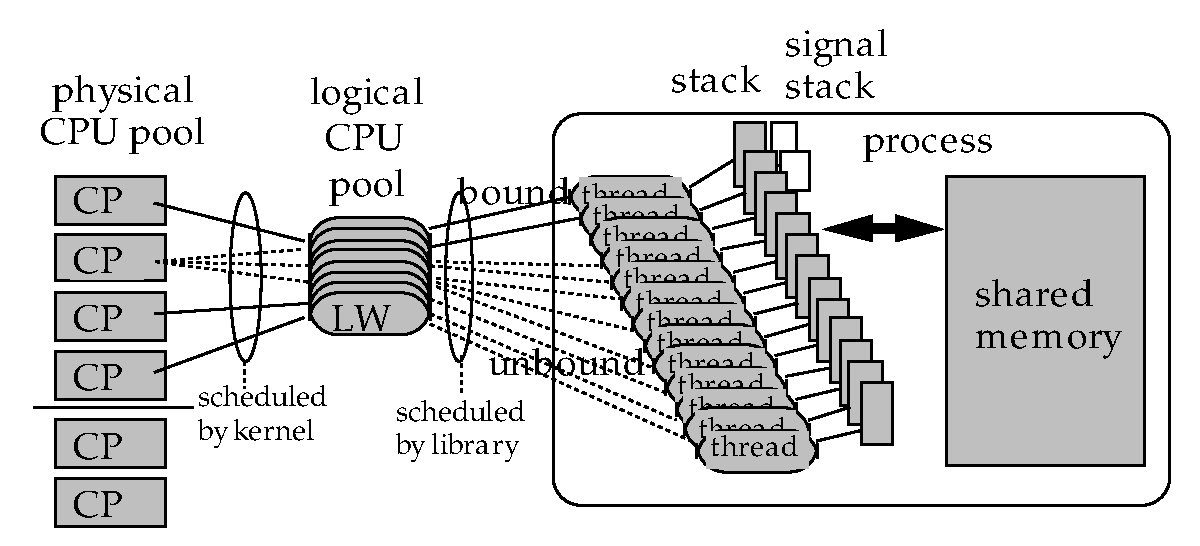
\includegraphics[width=130mm]{fig/threadfig.ps}
%\epsfile{file=fig/threadfig.ps,width=130mm}
\caption{Solarisオペレーティングシステムのスレッドモデル}\label{threadmodel}
\end{center}
\end{figure}

環境はC-stackとbinding-stackおよび{\tt lambda, block, catch, let, flet}
などのローカルブロックに繋がるフレームポインタにより構成されており、
新しいスレッドが作成されたときに設置される。
複数の環境が本当のマルチプロセッサマシンの上で同時に
動作できるので、グローバル変数の中の現在の環境に対して単一なポインタ
を持つことができない。
むしろ、環境のポインタを最上位の評価から低レベルのメモリ管理に変換するために、
すべての内部関数にもう一つ引き数を付け加えなければならない。

\subsubsection{メモリ管理}
EusLispは、すべての型のオブジェクトに対して単一のヒープの中で
フィボナッチバディを用いたメモリ管理方法を採用している。
異なったメモリ要求を持つプログラムを実行した後、
フィボナッチバディが様々な大きさのオブジェクトを等しく高速に配置することができ、コピーなしに素早くガーベージコレクトができ、
かつ、高いメモリ利用率(内部損失が10〜15\%で外部損失は無視できる)
を示すことを確信した。
マルチスレッドのためには、2つ目のポイントすなわちコピーなしの
ガーベージコレクトが重要である。
もし、オブジェクトのアドレスがガーベージコレクトのコピーにより
変化したならば、すべてのスレッド環境のスタックおよびCPUのレジスタ
内のポインタを新しいアドレスに書き換えなければならない。
しかし、この書き換えは不可能かあるいは大変困難である。

すべてのメモリ配置要求は、低レベルの{\tt alloc}関数によって処理される。
{\tt alloc}は、mutex-lockingをする。なぜなら、大きさを持たないリストの
グローバルデータベースを扱うからである。
ガーベージコレクトの始まる時期およびどのスレッドによってガーベージコレクトが
生じるのかを予言できないので、
すべてのスレッドは突発的に起こるガーベージコレクトのために
準備をしておかなければならない。
生きているオブジェクトへのすべてのポインタは、ゴミとして掃除されない
ように保護するためいつでもガーベージコレクトからアクセスできるよう
調整されなければならない。
これは、スタックの上に保存されていることを信用する代わりに、
それぞれの環境の固定されたスロットの中に極最近に配置されたオブジェクトに
対するポインタを蓄積することによって達成される。

図 \ref{parathreads}は、スレッドのメモリ要求とforkされたガーベージコレクト
内部でのmarkingおよびsweepingを並列に行っている流れ図を示したものである。
メモリ要求およびポインタの処理を行わないスレッドはガーベージコレクトと並列に
実行することができ、信号処理や画像獲得のような低レベルのタスクの
実時間応答を改善することに注意すること。

\begin{figure}
\begin{center}
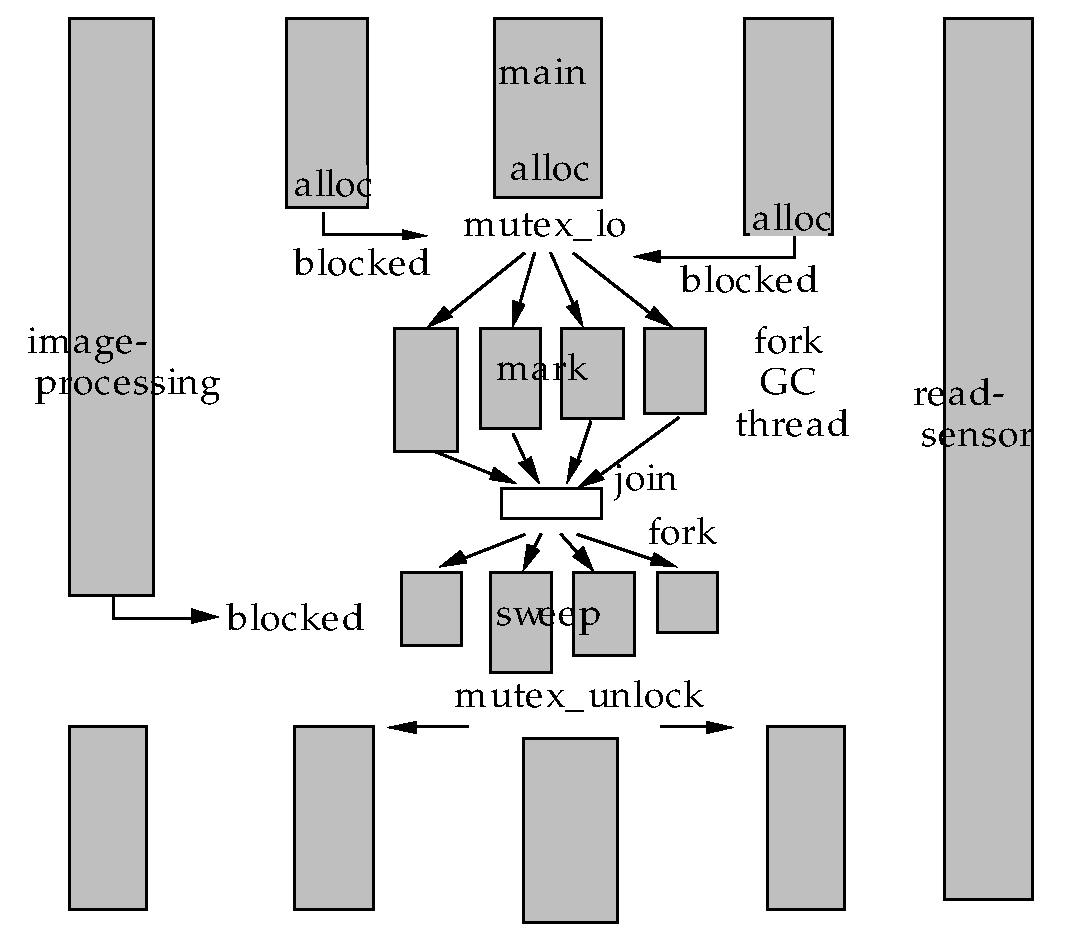
\includegraphics[width=120mm]{fig/parathreads.ps}
%\epsfile{file=fig/parathreads.ps,width=120mm}
\caption{並列スレッドのメモリ要求とガーベージコレクトに並列実行}\label{parathreads}
\end{center}
\end{figure}

\subsection{非同期プログラミングと並列プログラミングの構築}
\subsubsection{スレッド作成とスレッドプール}
Solarisにおいて複数のプロセッサ上で並列にプログラムを実行するためには、
そのプログラムは関数の集まりとして書かれる必要がある。
その関数はそれぞれプロセスの中で動的に作成されるスレッドによって
実行される。
スレッドを作成するために要求される時間は、プロセスを作成するよりも
速くなければならないが、スタックを配置しスタックのオーバーフローを
発見するためのページ属性を設定した後にスレッドが動き始めるまでに
Euslispにおいて数ミリ秒かかる。
この遅れは関数実施と比較して我慢できないため、
評価時間におけるシステムコールに対する所要時間を排除する目的で、
あらかじめ{\tt make-thread}関数により十分な数のスレッドが作られ、
システムのスレッドプールに置かれる。
スレッドプールの中のそれぞれのスレッドは、図\ref{threadobj}で示されるように
スレッドIDと同期のためのセマフォと引き数や評価結果を転送するためのスロット
から構成されるスレッドオブジェクトにより表現される。

\begin{figure}
\begin{center}
\begin{tabular}{c c}
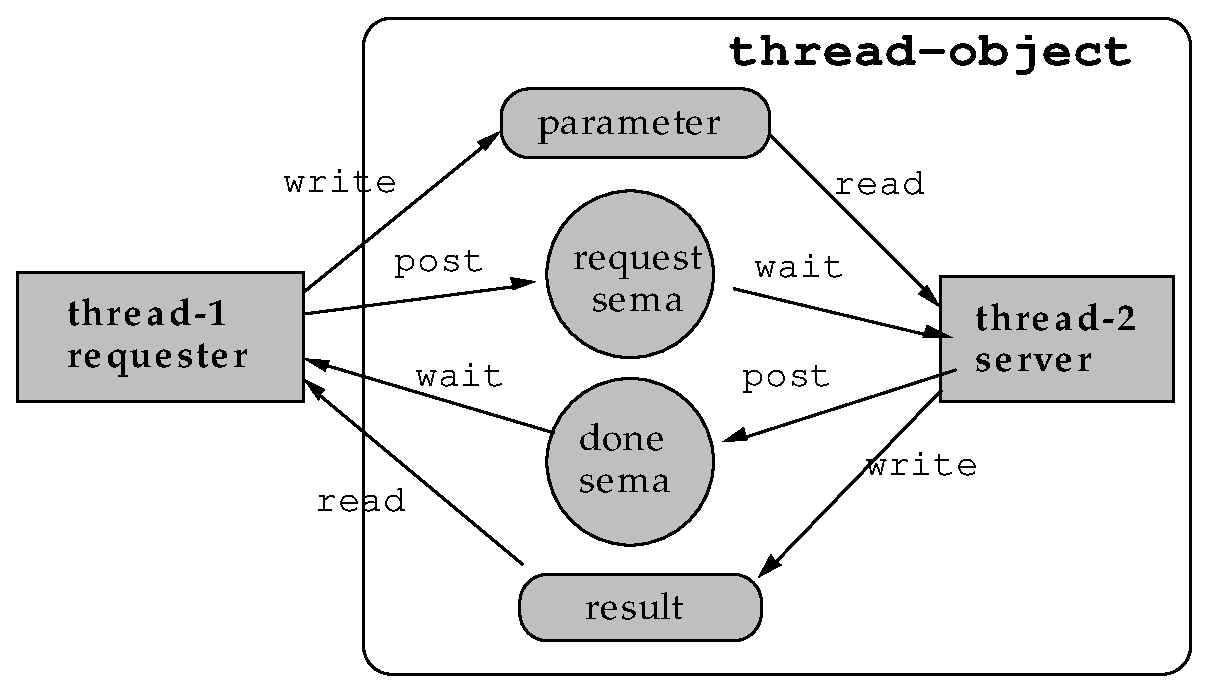
\includegraphics[width=7.5cm]{fig/threadobj.ps} &
%\epsfile{file=fig/threadobj.ps,width=7.5cm} &
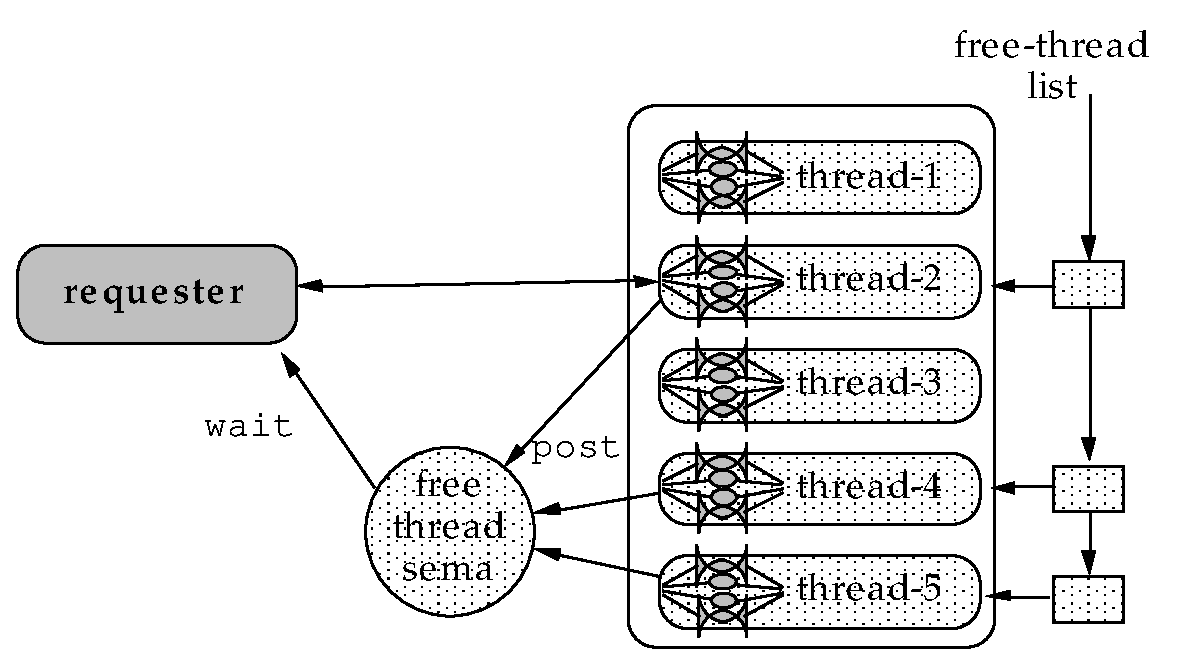
\includegraphics[width=7.5cm]{fig/threadpool.ps} \\
%\epsfile{file=fig/threadpool.ps,width=7.5cm} \\
\end{tabular}
\end{center}
\caption{\label{threadobj}スレッド間で制御やデータを受け渡すためのスレッドオブジェクト(左)とスレッドプール内に置かれたスレッドの集まり(右)}
\end{figure}

\subsubsection{スレッドの並列実行}
スレッドによる並列実行の配置のために、スレッド関数が使用される。
スレッドは、スレッドプールから1つの空きスレッドを取り、
共有メモリを経由して引き数を渡し、図\ref{threadobj}に示されるような
セマフォ信号によりスレッドを立ち上げ、
停止することなしに呼出側へスレッドオブジェクトを返す。
立ち上げられたスレッドは、呼び出したスレッドと並列に実行され、
引き数を評価し始める。
呼出側は、forkされたスレッドから評価結果を受けとるために{\tt wait-thread}を
使用する。
{\tt plist}マクロは、引き数の並列評価を記述するために大変便利な書式である。
{\tt plist}は、それぞれの引き数を評価するためにスレッドを割り当て、
すべてのスレッドが評価し終わるのを待って結果をリストアップする。

\subsubsection{同期の手法}
MT-Eusは、{\bf mutex lock, condition variable, セマフォ}と呼ばれる
3種類の同期手法を持っている。
mutex lockは、スレッド間の共有変数の連続アクセスのために使用される。
condition variableは、ロックの仮開放あるいは再獲得によってmutex-lockされた
部分の条件がtrueになることを待つことをスレッドに許可する。
セマフォは、イベントの発生を通知するためあるいはリソースの分割を制御するために
使用される。
Solarisのカーネルが時間分割スケージューリングを基本として何気なしにタスク
切り替えを発生するのと異なり、
これらの同期手法は、任意の環境切り替えを引き起こす。

\begin{figure}
\begin{center}
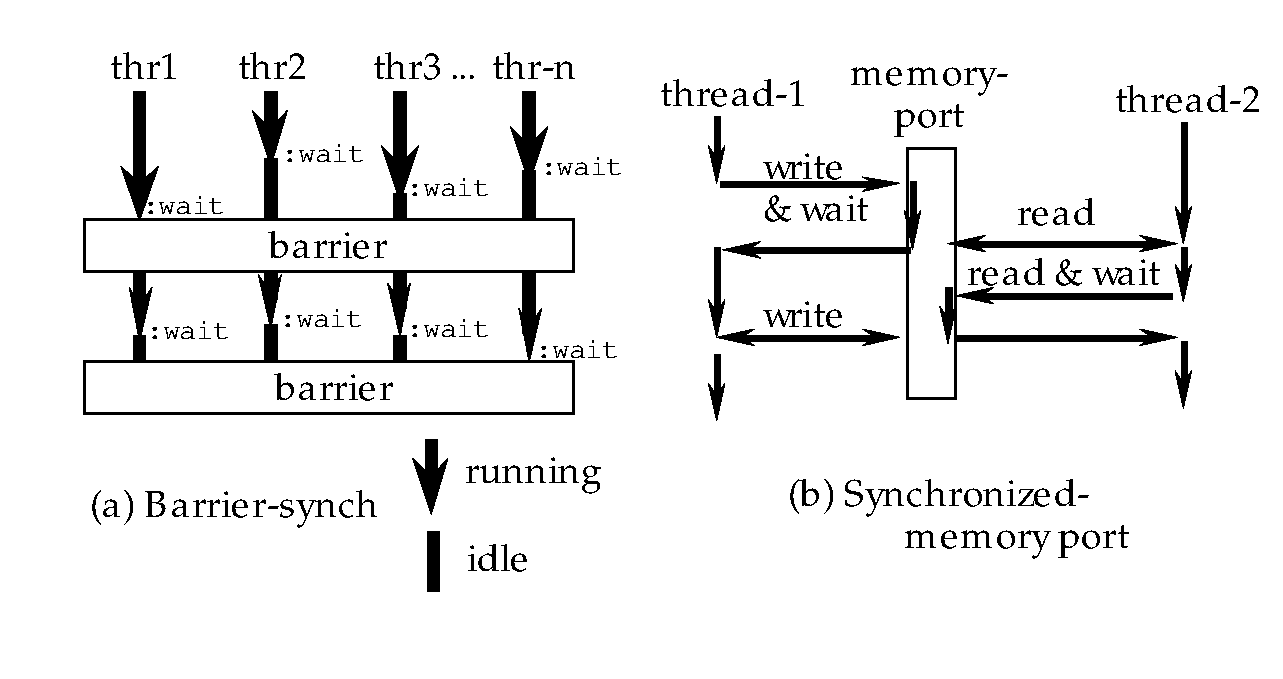
\includegraphics[width=130mm]{fig/synchports.ps}
%\epsfile{file=fig/synchports.ps,width=130mm}
\caption{同期障壁と同期メモリポート}
\label{synchports}
\end{center}
\end{figure}

\subsubsection{同期障壁}
{\bf barrier-synch}は、複数のスレッドを同時に同期させるための機構である
(図 \ref{synchports})。
この目的において、{\bf barrier}クラスのインスタンスが作成され、
同期に関係するスレッドがオブジェクトに登録される。
その後、それぞれのスレッドはbarrierオブジェクトに{\tt :wait}メッセージを
送り、そのスレッドは停止する。
オブジェクトに登録された最後のスレッドが{\tt :wait}メッセージを送ったとき、
待ちが解除され、すべての待ちスレッドがTの返り値を得る。
barrier-syncは、マルチロボットシミュレーションのグローバルタイムという
重要な役割を演じている。

\subsubsection{同期メモリポート}
{\bf 同期メモリポート(synch-memory-port)}は、
スレッド間でデータを交換するための1種のストリーム
である(図 \ref{synchports})。
プロセス内のすべてのスレッドはヒープメモリを共有しているので、
もし1つのスレッドがグローバル変数にオブジェクトを割り当てた場合、
直ちに他のスレッドから見れるようになる。
しかしながら、共有メモリはグローバルデータが更新されたという
イベントを送るための能力が不足している。
同期メモリポートは、共有オブジェクトをアクセスするための
この同期機能を保証する。
同期メモリポートオブジェクトは、1つのバッファスロットと同期読み書きの
ために使用される2つのセマフォによって構成されている。

\subsubsection{タイマー}
実時間プログラムは、予定された時間に実行される関数や、
特定の間隔で繰り返される関数をしばしば要求する。
これまでのEusLispは、Unixのインターバルタイマーによって
定期的に生成される信号によって発生するユーザー関数を
実行することができた。
MT-Eusにおいて、この実行はデッドロックを引き起こす。
なぜなら、割り込みがmutex-lockされたブロック内から発生する可能性がある。
したがって、制御は{\tt eval}の最初のように安全な場所で渡されなければ
ならない。
上記の同期によって引き起こされる遅れを避けるために、
MT-Eusはセマフォを経由して信号通知(signal-notification)も
提供する。
言い換えれば、信号関数は呼び出されるかあるいは信号の到着を知らせる
関数あるいはセマフォのどちらかをとる。
セマフォは、低レベルで告示されるので、
同期により隠れているところは最小である。

以下に示すものは、マルチスレッド機能を用いた画像処理のプログラム例である。
画像入力スレッドとフィルタースレッドが生成される。
samp-imageは、33msec毎に通知されるsamp-semを待つことにより、
定期的に画像データをとる。
2つのスレッドはthread-portの読み書きを通じて同期する。
filter-imageは、フィルターの並列計算のために複数のスレッドを使用している。

\begin{quote}
\begin{verbatim}
(make-threads 8)
(defun samp-image (p)
   (let ((samp-sem (make-semaphore)))
        (periodic-sema-post 0.03 samp-sem)
        (loop (sema-wait samp-sem)
              (send p :write (read-image))))
(defun filter-image (p)
  (let (img)
       (loop (setf img (send p :read))
             (plist (filter-up-half img)
                    (filter-low-half img)))))
(setf port (make-thread-port))
(setf sampler (thread #'samp-image port))
(setf filter (thread #'filter-image port))
\end{verbatim}
\end{quote}

\subsection{並列度の計測}

表 \ref{paragain}は、32CPUで構成されるCray Superserverの上で測定
した並列実行効率を示したものである。
コンパイルされたフィボナッチ関数において線形な並列度が得られた。
なぜなら、共有メモリへのアクセスがなく、それぞれのプロセッサのキャッシュ
メモリに十分ロードできるほどちいさなプログラムであったためである。
それに反して、同じプログラムをインタープリターで実行したとき、
キャッシュメモリを使い果たしたため、
線形な高効率を達成することができなかった。
さらにまた、頻繁に共有メモリを参照するようなプログラムや
メモリ配置を要求するようなプログラムは1個のプロセッサで実行した
ときよりも良い性能を得ることができなかった。
これは、頻繁なキャッシュメモリの入れ替えが原因と考えられる。

\begin{table}
\caption{\label{paragain}マルチプロセッサ上で実行されたプログラムの並列度}
\begin{center}
\begin{tabular}{|l|r|r|r|r|c|}  \hline
processors & 1 & 2 & 4 & 8 & GC (ratio) \\ \hline
(a) compiled Fibonacci & 1.0 & 2.0 & 4.0 & 7.8 & 0 \\ \hline
(b) interpreted Fibonacci & 1.0 & 1.7 & 2.7 & 4.4 & 0 \\ \hline
(c) copy-seq & 1.0 & 1.3 & 0.76 & 0.71 & 0.15 \\ \hline
(d) make-cube & 1.0 & 0.91 & 0.40 & 0.39 &  0.15 \\ \hline
(e) interference-check & 1.0 & 0.88 & 0.55 & 0.34 & 0.21 \\ \hline
\end{tabular} \\
\end{center}
\end{table}

\subsection{スレッド生成}
スレッドは、計算を割り当てる単位であり、普通lisp書式を評価する
ための単位である。
Euslispのスレッドは、{\bf thread}クラスのインスタンスによって
表現される。
このオブジェクトは、内容を表現するスレッド全体というよりはむしろ、
実際に引き数と結果を渡すためのスレッドの
制御ポートであり、評価を始めるものである。

\begin{refdesc}

\funcdesc{sys:make-thread}{num \&optional (lsize 32*1024) (csize lsize)}{
{\em lsize}ワードのlispスタックと{\em csize}ワードのC-スタックを持つ
スレッドを{\em num}個だけ生成し、システムのスレッドプールに
置く。
スレッドプール内のすべてのスレッドは、sys:*threads*に束ねてあり、
{\bf make-thread}が呼び出されたときに拡張される。
{\bf thread}関数によって、計算はスレッドプールの中で空いたスレッドの
1つに割り当てられる。
したがって、指定された計算がどのスレッドに割り当てられるか
制御できないため、スレッドのスタックサイズを変更する方法が無い。}

\vardesc{sys:*threads*}{
{\bf make-thread}によって作成されたすべてのスレッドのリストを持つ。}

\funcdesc{sys::free-threads}{}{
スレッドプール内の空いたスレッドのリストを返す。
もし、結果がNILならば、スレッドへのタスクの新しい付託は現在実行されている
スレッドのどれかの評価が終了するかあるいは
{\bf make-thread}によってスレッドプールに新しいスレッドを生成するまで
停止される。}

\funcdesc{sys:thread}{func \&rest args}{
スレッドプールから空いたスレッドを1つ取り出し、
{\em (func . args)}の評価のためにそれを割り当てる。
{\bf sys:thread}は、{\em args}を展開したリストに{\rm func}を適用
するが、関数の適用結果を受け取らないため、
非同期の{\bf funcall}とみなすことができる。
むしろ、{\bf sys:thread}はfuncallに割り当てられたスレッド
オブジェクトを返すので、実際の結果は{\bf sys:wait-thread}によって
後から得ることができる。}
\begin{quote}
\begin{verbatim}
(defun compute-pi (digits) ...)
(setq trd (sys:thread \#'compute-pi 1000)) ;assign compute-pi to a thread
...  ;; other computation 
(sys:wait-thread trd) ;get the result of (compute-pi 1000)
\end{verbatim}
\end{quote}

\funcdesc{sys:thread-no-wait}{func \&rest args}{
空いたスレッドの1つに計算を割り当てる。
スレッドは、{\bf wait-thread}されることなしに、
評価が終了したとき、スレッドプールに戻される。}

\funcdesc{sys:wait-thread}{thread}{
{\em thread}に{\bf sys:thread}関数によって与えられたfuncallの評価が
終了するのを待ち、その結果を受け取り、返す。
もし、スレッドに{\bf sys:thread}によって評価が割り当てられたならば、
{\bf sys:wait-thread}は、必須である。
なぜなら、スレッドは結果を転送し終わるまでスレッドプールに戻らない
ためである。}
 
\macrodesc{sys:plist}{\&rest forms}{
異なったスレッドにより並列に{\em forms}を評価し、
すべての評価が終了するのを待ち、
結果のリストを返す。
{\bf sys:plist}は、リスト化されたそれぞれのformが関数呼び出しされる
ことを除いて、{\em parallel-list}としてみなされるだろう。}

\end{refdesc}

\subsection{同期}

Solarisオペレーティングシステム内には、マルチスレッドプログラムのために
4つの同期手法がある。
Euslispは、mutex-lockとcondition variableとセマフォを提供している。
reader-writer lockは実現されてない。
これらの手法に基づいて、同期メモリポートや同期障壁のような
高レベルの同期機構が実現されている。

\begin{refdesc}
\funcdesc{sys:make-mutex-lock}{}{
mutex-lockを作り、返す。
mutex-lockは、6つの要素を持つ整数ベクトルで表現されている。}

\funcdesc{sys:mutex-lock}{mlock}{
mutex-lockの{\em mlock}をロックする。
もし、{\em mlock}が既に他のスレッドからロックされているなら、
{\bf mutex-lock}はロックが外されるまで待つ。}

\funcdesc{sys:mutex-unlock}{mlock}{
{\em mlock}を解除し、このロックを待っている他のスレッドの内の1つが再び実行され始める。}

\macrodesc{sys:mutex}{mlock \&rest forms}{
mutex-lockとmutex-unlockは、組みで使用されなければならない。
{\bf mutex}は、重要な部分をひとまとまりにしたマクロである。
{\em mlock}は、評価する{\em forms}が評価される前にロックされる。
そして、評価が終了したときに、ロックが解除される。
このマクロは、以下のprogn formに展開される。
{\bf unwind-protect}は、{\em forms}の評価中にエラーが発生したとき
でさえ、ロックの解除を保証するために使用されることに注意すること。
}
\begin{quote}
\begin{verbatim}
  (progn
      (sys:mutex-lock mlock)
      (unwind-protect
          (progn . forms)
          (sys:mutex-unlock mlock)))
\end{verbatim}
\end{quote}

\funcdesc{sys:make-cond}{}{
4つの要素を持つ整数ベクトルであるcondition variableオブジェクトを
作る。condition variableの返り値としては、ロックされてない状態でである。}

\funcdesc{sys:cond-wait}{condvar mlock}{
{\em condvar}に信号が出されるまで待つ。
もし、{\em condvar}が他のスレッドによってすでに獲得されていたならば、
{\em mlock}を解除し、{\em condvar}に信号が出されるまで待つ。}

\funcdesc{sys:cond-signal}{condvar}{
{\em condvar}で示されるcondition variableに信号を出す。}
\funcdesc{sys:make-semaphore}{}{
20の要素を持つ整数ベクトルによって表現されるセマフォオブジェクトを作る。}
\funcdesc{sys:sema-post}{sem}{{\em sem}に信号を出す。}
\funcdesc{sys:sema-wait}{sem}{
{\em sem}に信号が来るまで待つ。}

\classdesc{sys:barrier-synch}{propertied-object}{
threads n-threads count barrier-cond threads-lock count-lock}
{同期障壁のための構造を表現する。
同期を待っているスレッドは、{\em thread-lock}によって
相互に排除される{\em thread}に置かれる。
{\bf barrier-synch}オブジェクトが生成されたとき、
{\em count}は、ゼロに初期化される。
同期しているスレッドは、{\tt :add}メッセージを送ることによって、
{\em threads}リストに置かれる。
このbarrier-synchオブジェクトに{\tt :wait}を送ることは、
{\em count}を増加させることの原因となり、
送られたスレッドは待ち状態になる。
{\em threads}の中のすべてのスレッドに{\tt :wait}メッセージが送られたとき、
待ちが解除され、すべてのスレッドの実行が再び始まる。
同期は、{\em count-lock}のmutex-lockと{\em barrier-cond}のcondition-variable
の組み合わせによって実行される。}

\methoddesc{:init}{}{このbarrier-synchオブジェクトを初期化する。
2つのmutex-lockと1つのcondition-variableが生成される。}
\methoddesc{:add}{thr}{{\em threads}リストの中に{\em thr}スレッドが追加される。}
\methoddesc{:remove}{thr}{{\em threads}リストの中から{\em thr}スレッドを削除する。}
\methoddesc{:wait}{}{{\em threads}リストの中のすべてのスレッドに{\tt :wait}
が配布されるのを待つ。}

\classdesc{sys:synch-memory-port}{propertied-object}{
sema-in sema-out buf empty lock}{
1方向の同期されたメモリポートを実現する。
このオブジェクトを通じてデータを転送するために、2つのスレッドを同期させる。
転送制御は、セマフォを用いて実現されている。}

\methoddesc{:read}{}{
この{\bf synch-memory-port}にバッファされているデータを読む。
もし、まだ書かれていなかったならば、{\tt :read}は停止する。}

\methoddesc{:write}{datum}{
バッファに{\em datum}を書き込む。
1ワードのバッファのみ存在するので、
もし他のデータが既に書かれておりまだ読まれていなかったならば、
{\tt :write}は{\tt :read}によってそのデータが読み込まれるまで待つ。}

\methoddesc{:init}{}{この{\bf sync-memory-port}を初期化する。
これには2つのセマフォが生成され、{\tt :write}動作が可能な状態になっている。}

\end{refdesc}

\newpage

\section{幾何学関数}
\markright{\arabic{section}. 幾何学関数}

\subsection{実数ベクトル(float-vector)}

float-vectorは、要素が実数である1次元ベクトルである。
float-vectorは、どんなサイズでも良い。
{\em result}が引き数リストで指定されているとき、
その{\em result}はfloat-vectorであるべきである。

\begin{refdesc}

\funcdesc{float-vector}{\&rest numbers}{
{\em numbers}を要素とするfloat-vectorを新しく作る。
{\tt (float-vector 1 2 3)}と{\tt \#F(1 2 3)}の違いに注意すること。
前者は、呼ばれたときはいつでもベクトルが生成されるが、
後者は読み込まれたときのみ生成される。}

\funcdesc{float-vector-p}{obj}{
{\em obj}がfloat-vectorであるならば、Tを返す。}

\funcdesc{v+}{fltvec1 fltvec2 \&optional result}{
2つのfloat-vectorを加える。}

\funcdesc{v-}{fltvec1 \&optional fltvec2  result}{
2つのfloat-vectorを差し引く。もし、{\em fltvec2}が省略されているならば、
{\em fltvec1}の符号が反転される。}

\funcdesc{v.}{fltvec1 fltvec2}{2つのfloat-vectorの内積を計算する。}

\funcdesc{v*}{fltvec1 fltvec2 \&optional result}{
2つのfloat-vectorの外積を計算する。}

\funcdesc{v.*}{fltvec1 fltvec2 fltvec3}{
スカラー3重積を計算する。{\tt (v.* A B C)=(V. A (V* B C))=(V. (V* A B) C)}}

\funcdesc{v$<$}{fltvec1 fltvec2}{
もし、{\em fltvec1}の要素が{\em fltvec2}の対応する要素よりすべて小さいとき、
Tを返す。}

\funcdesc{v$>$}{fltvec1 fltvec2}{
もし、{\em fltvec1}の要素が{\em fltvec2}の対応する要素よりすべて大きいとき、
Tを返す。}

\funcdesc{vmin}{\&rest fltvec}{
{\em fltvec}の中のそれぞれの次元における最小値を捜し、
その値でfloat-vectorを新しく作る。{\bf vmin}と{\bf vmax}は、
頂点の座標から最小のminimal-boxを見つけるために使用される。}

\funcdesc{vmax}{\&rest fltvec}{
{\em fltvec}の中のそれぞれの次元における最大値を捜し、
その値でfloat-vectorを新しく作る。}

\funcdesc{minimal-box}{v-list minvec maxvec [err]}{
与えられた{\em v-list}に対して{\tt minimal bounding box}を計算し、
その結果を{\em minvec}と{\em maxvec}に蓄積する。
もし、実数{\em err}が指定されているならば、{\tt minimal box}はその比率によって
成長する。すなわち、もし{\em err}が0.01のとき、{\em minvec}のそれぞれの
要素は{\em minvec}と{\em maxvec}との距離の1\%減少する。
そして、{\em maxvec}のそれぞれの要素は1\%増加する。
{\bf minimal-box}は、{\em minvec}と{\em maxvec}との距離を返す。}

\funcdesc{scale}{number fltvec \&optional result}{
{\em fltvec}のすべての要素をスカラー{\em number}倍する。}

\funcdesc{norm}{fltvec}{{\em fltvec}のノルムを求める。{\tt $\Vert fltvec\Vert$}}
\funcdesc{norm2}{fltvec}{{\em fltvec}のノルムの2乗を求める。
{\tt $\Vert fltvec\Vert^2$=(v. fltvec fltvec)}}
\funcdesc{normalize-vector}{fltvec \&optional result}{
{\em fltvec}のノルムが1.0となるように正規化する。}
\funcdesc{distance}{fltvec1 fltvec2}{
2つのfloat-vectorの距離を返す。$|fltvec-fltvec2|$}
\funcdesc{distance2}{fltvec1 fltvec2}{
2つのfloat-vectorの距離の2乗を返す。$|fltvec-fltvec2|^2$}

\funcdesc{homo2normal}{homovec \&optional normalvec}{
同次ベクトル{\em homovec}を正規表現に変換する。}

\funcdesc{homogenize}{normalvec \&optional homovec}{
正規ベクトル{\em normalvec}を同次表現に変換する。}

\funcdesc{midpoint}{p p1 p2 \&optional result}{
{\em p}は実数で、{\em p1,p2}は同次元のfloat-vectorである。
{\em p1$-$p2}を$p:(1-p)$の比率で等分した点$(1-p)\cdot p1 + p\cdot p2$
を返す。}

\funcdesc{rotate-vector}{fltvec theta axis \&optional result}{
2次元あるいは3次元の{\em fltvec}を{\em axis}回りに{\em theta}ラジアン
回転する。
{\em axis}は、{\em :x, :y, :z, 0, 1, 2}, または NILの内の一つである。
{\em axis}がNILのとき、{\em fltvec}は2次元として扱われる。
3次元空間の任意の軸の回りにベクトルを回転するためには、
{\bf rotation-matrix}で回転行列を作り、そのベクトルにかければよい。}

\end{refdesc}

\subsection{行列と変換}

行列は、要素がすべて実数の2次元の配列である。
ほとんどの関数において行列はどんなサイズでもよいが、
{\bf v*, v.*, euler-angle, rpy-angle}関数では3次元の行列のみ
扱うことができる。
{\bf transform, m*}と{\bf transpose}は、行列を正方行列に限定せず、
一般のn*m行列に対して処理を行う。

{\em result}パラメータを受けた関数は、計算結果をそこに置く。
そのため、ヒープは使用しない。
すべての行列関数は、正規座標系における変換を考慮しており、
同次座標系は考慮していない。

{\bf rpy-angle}関数は、回転行列をワールド座標系におけるz,y,x軸回りの
3つの回転角に分解する。
{\bf euler-angle}関数は{\bf rpy-angle}と同様に分解するが、
回転軸がローカル座標系のz,y,z軸となっている。
角度が反対方向にも得られるため、これらの関数は2つの解を返す。

\begin{verbatim}
; Mat is a 3X3 rotation matrix.
(setq rots (rpy-angle mat))
(setq r (unit-matrix 3))
(rotate-matrix r (car rots) :x t r)
(rotate-matrix r (cadr rots) :y t r)
(rotate-matrix r (caddr rots) :z t r)
;--> resulted r is equivalent to mat
\end{verbatim}

3次元空間の位置と方向の組みを保つために、\ref{Coordinates}節に記載されている
{\bf coordinates}と{\bf cascaded-coords}クラスを使用すること。

\begin{refdesc}
\funcdesc{matrix}{\&rest elements}{
{\em elements}から行列を新しく作る。
{\tt Row x Col = (elementsの数) x (最初のelementの長さ)}
{\em elements}は、どの型の列((list 1 2 3)や(vector 1 2 3)や
(float-vector 1 2 3))でもよい。
それぞれの列は行列の行ベクトルとしてならべられる。}

\funcdesc{make-matrix}{rowsize columnsize \&optional init}{
$rowsize \times columnsize$の大きさの行列を作る。}

\funcdesc{matrixp}{obj}{
もし、{\em obj}が行列のとき、すなわち、{\em obj}が2次元の配列で
その要素が実数であるとき、Tを返す。}

\funcdesc{matrix-row}{mat row-index}{
行列{\em mat}から{\em row-index}で示される行ベクトルを抽出する。
{\bf matrix-row}は、{\bf setf}を使用することにより
行列の特定の行にベクトルを設定することにも使用される。}
\funcdesc{matrix-column}{mat column-index}{
行列{\em mat}から{\em coloumn-index}で示される列ベクトルを抽出する。
{\bf matrix-column}は、{\bf setf}を使用することにより
行列の特定の列にベクトルを設定することにも使用される。}
\funcdesc{m*}{matrix1 matrix2 \&optional result}{
{\em matrix1}と{\em matrix2}の積を返す。}
\funcdesc{transpose}{matrix \&optional result}{
{\em matrix}の転置行列を返す。すなわち、{\em matrix}の列と行を入れ替える。}
\funcdesc{unit-matrix}{dim}{
{\em dim} $\times$ {\em dim}の単位行列を作る。}
\funcdesc{replace-matrix}{dest src}{
行列{\em dest}のすべての要素を同一な行列{\em src}で置き換える。}

\funcdesc{scale-matrix}{scalar mat}{
{\em mat}のすべての要素に{\em scaler}を掛ける。}

\funcdesc{copy-matrix}{matrix}{
{\em matrix}のコピーを作る。}

\funcdesc{transform}{matrix fltvector \&optional result}{
行列{\em matrix}をベクトル{\em fltvector}の左から掛ける。}
\funcdesc{transform}{fltvector matrix \&optional result}{
行列{\em matrix}をベクトル{\em fltvector}の右から掛ける。}

\funcdesc{rotate-matrix}{matrix theta axis \&optional world-p result}{
{\bf rotate-matrix}で行列{\em matrix}を回転させるとき、
回転軸({\bf :x, :y, :z}または0,1,2)はワールド座標系あるいは
ローカル座標系のどちらかを与えられる。
もし、{\em world-p}にNILが指定されているとき、
ローカル座標系の軸に沿った回転を意味し、回転行列を左から掛ける。
もし、{\em world-p}がnon-NILのとき、
ワールド座標系に対する回転行列を作り、回転行列を右から掛ける。
もし、{\em axis}にNILが与えられたとき、行列{\em matrix}は2次元と仮定され、
{\em world-p}の如何にかかわらず2次元空間の回転が与えられる。}


\funcdesc{rotation-matrix}{theta axis \&optional result}{
{\em axis}軸回りの2次元あるいは3次元の回転行列を作る。
軸は:x,:y,:z,0,1,2,3次元ベクトルあるいはNILのどれかである。
2次元回転行列を作るとき、{\em axis}はNILでなければならない。}

\funcdesc{rotation-angle}{rotation-matrix}{
{\em rotation-matrix}から等価な回転軸と角度を抽出し、
実数とfloat-vectorのリストを返す。
{\em rotation-matrix}が単位行列のとき、NILが返される。
また、回転角が小さいとき、結果がエラーとなる。
{\em rotation-matrix}が2次元のとき、1つの角度値が返される。}

\funcdesc{rpy-matrix}{ang-z ang-y ang-x}{
ロール、ピッチ、ヨー角で定義される回転行列を作る。
最初に、単位行列をx軸回りに{\em ang-x}ラジアン回転させる。
次に、y軸回りに{\em ang-y}ラジアン、最後にz軸回りに{\em ang-z}
ラジアン回転させる。
すべての回転軸はワールド座標系で与えられる。}

\funcdesc{rpy-angle}{matrix}{
{\em matrix}の2組のロール、ピッチ、ヨー角を抽出する。}

\funcdesc{Euler-matrix}{ang-z ang-y ang2-z}{
3つのオイラー角で定義される回転行列を作る。
最初に単位行列をz軸回りに{\em ang-z}回転させ、次にy軸回りに{\em ang-y}
回転させ、最後にz軸回りに{\em ang2-z}回転させる。
すべての回転軸はローカル座標系で与えられる。}

\funcdesc{Euler-angle}{matrix}{
{\em matrix}から2組のオイラー角を抽出する。}

%\funcdesc{set-matrix-row}{mat row-index values}{
%puts values in the {\em row-index}th row of matrix {\em mat}.}

%\funcdesc{set-matrix-column}{mat column-index values}{
%put values in the {\em column-index}th column of of matrix {\em mat}.}
\end{refdesc}

\subsection{LU分解}
{\bf lu-decompose}と{\bf lu-solve}は、線形の連立方程式を
解くために用意されている。
最初に、{\bf lu-decompose}は行列を下三角行列を上三角行列に分解する。
もし、行列が特異値なら、{\bf lu-decompose}はNILを返す。
そうでなければ、{\bf lu-solve}に与えるべき順列ベクトルを返す。
{\bf lu-solve}は、与えられた定数ベクトルの解をLU行列で計算する。
この手法は、同じ係数行列と異なった定数ベクトルのたくさんの組に対して
解を求めたいときに効果的である。
%These functions are coded in C, and they computes a solution
%for a 3*3 matrix within 3 milli-sec on sun3.
{\bf simultaneous-equation}は、1つの解だけを求めたいときにもっとも
手軽な関数である。
{\bf lu-determinant}は、LU分解された行列の行列式を計算する。
{\bf inverse-matrix}関数は、{\bf lu-decompose}を1回と{\bf lu-solve}をn回
使って逆行列を求める。
3*3行列での計算時間は約4msである。

\begin{refdesc}

\funcdesc{lu-decompose}{matrix \&optional result}{
{\em matrix}にLU分解を実行する。}

\funcdesc{lu-solve}{lu-mat perm-vector bvector [result]}{
LU分解された1次連立方程式を解く。
{\em perm-vector}は、{\bf lu-decompose}で返された結果でなければならない。}

\funcdesc{lu-determinant}{lu-mat perm-vector}{
LU分解された行列の行列式を求める。}

\funcdesc{simultaneous-equation}{mat vec}{
係数が{\em mat}で、定数が{\em vec}で記述される1次連立方程式を解く。}

\funcdesc{inverse-matrix}{mat}{
正方行列{\em mat}の逆行列を求める。}

\funcdesc{pseudo-inverse}{mat}{
特異値分解を用いて擬似逆行列を求める。}

\end{refdesc}

\newpage

\subsection{\label{Coordinates}座標系}

座標系と座標変換は、{\bf coordinates}クラスで表現される。
4*4の同次行列表現の代わりに、
Euslisp内で座標系は、高速性と一般性のために
3*3の回転行列と3次元位置ベクトルの組で表現される。

\begin{refdesc}

\classdesc{coordinates}{propertied-object}
{(pos :type float-vector \\
\>  rot :type array)}
{位置ベクトルと3x3の回転行列の組みで座標系を定義する。}

\funcdesc{coordinates-p}{obj}{
{\em obj}が{\bf coordinates}クラスかまたはそのサブクラスのインスタンス
のとき、Tを返す。}

\methoddesc{:rot}{}{
この座標系の3x3回転行列を返す。}

\methoddesc{:pos}{}{
この座標系の3次元位置ベクトルを返す。}

\methoddesc{:newcoords}{newrot \&optional newpos}{
{\em newrot}と{\em newpos}でこの座標系を更新する。
{\em newpos}が省略された時は{\em newrot}にはcoordinatesのインスタンスを
与える。
この座標系の状態が変化するときはいつでも、このメソッドを用いて新しい
回転行列と位置ベクトルに更新するべきである。
このメッセージはイベントを伝えて他の{\bf :update}メソッドを呼び出す。}

\methoddesc{:replace-coords}{newrot \&optional newpos}{
{\em :newcoords}メソッドを呼び出さずに{\tt rot}と{\tt pos}スロットを変更する。
{\em newpos}が省略された時は{\em newrot}にはcoordinatesのインスタンスを与える。}
\metdesc{:coords}{}

\methoddesc{:copy-coords}{\&optional dest}{
もし{\em dest}が与えられなかったとき、{\bf :copy-coords}は同じ{\tt rot}と{\tt pos}
スロットを持つ座標系オブジェクトを作る。
もし、{\em dest}が与えられたとき、{\em dest}座標系にこの座標系のrotとposを
コピーする。}

\methoddesc{:reset-coords}{}{
この座標系の回転行列を単位行列にし、位置ベクトルをすべてゼロにする。}

\metdesc{:worldpos}{}
\metdesc{:worldrot}{}
\methoddesc{:worldcoords}{}{
このオブジェクトのワールド座標系における位置ベクトル・回転行列・座標系
を計算する。
その座標系は、いつもワールド座標系で表現されていると仮定され、
これらのメソッドは簡単に{\tt pos}と{\tt rot}と{\tt self}を返すことができる。
これらのメソッドは{\bf cascaded-coords}クラスと互換性がとられている。
{\bf cascaded-coords}ではワールド座標系での表現と仮定していない。}

\methoddesc{:copy-worldcoords}{\&optional dest}{
最初に、ワールド座標系が計算され、{\em dest}にコピーされる。
もし、{\em dest}が指定されてないとき、新たに{\bf coordinates}
オブジェクトを作る。}

\methoddesc{:rotate-vector}{vec}{
この座標系の回転行列によって{\em vec}を回転させる。すなわち、
この座標系で表現される方向ベクトルをワールド座標系における表現
に変換する。
この座標系の位置は、回転に影響を与えない。}

\methoddesc{:transform-vector}{vec}{
この座標系で表現される{\em vec}をワールド座標系の表現に変換する。}

\methoddesc{:inverse-transform-vector}{vec}{
ワールド座標系における{\em vec}をローカル座標系の表現に逆変換する。}

\methoddesc{:transform}{ trans \&optional (wrt :local)}{
{\em wrt}座標系で表現される{\em trans}によってこの座標系を変換する。
{\em trans}は座標系の型でなければならないし、{\em wrt}は
{\tt :local, :parent, :world}のキーワードあるいは{\bf coordinates}の
インスタンスでなければならない。
もし{\em wrt}が{\tt :local}のとき、{\em trans}をこの座標系の右
から適用する。もし{\em wrt}が{\tt :world, :parent}のとき、
{\em trans}を左から掛ける。
もし{\em wrt}が{\bf coordinates}の型であるとき、{\em wrt}座標系で表現される
{\em trans}は最初にワールド座標系の表現に変換され、左から掛ける。}

\methoddesc{:move-to}{trans \&optional (wrt :local)}{
{\em wrt}で表現される{\em trans}でこの座標系の{\tt rot}と{\tt pos}
を置き換える。}

\methoddesc{:translate}{ p \&optional (wrt :local)}{
このオブジェクトの位置を{\em wrt}座標系で相対的に変更する。}

\methoddesc{:locate}{ p \&optional (wrt :local)}{
この座標系の位置を{\em wrt}座標系で絶対的に変更する。
もし、{\em wrt}が{\tt :local}のとき、{\bf :translate}と同一な
効果を生む。}

\methoddesc{:rotate}{ theta axis \&optional (wrt :local)}{
{\em axis}軸回りに{\em theta}ラジアンだけ相対的にこの座標系を回転させる。
{\em axis}は、軸キーワード({\tt :x, :y, :z})あるいは任意の{\tt float-vector}
である。
{\em axis}は{\em wrt}座標系で表現されていると考える。
よって、もし{\em wrt}が{\tt :local}で{\em axis}が{\tt :z}であるとき、
座標系はローカル座標系のz軸回りに回転される。
もし{\em wrt}が{\tt :world, :parent}であるとき、ワールド座標系のz軸回りに
回転される。
言い換えると、もし{\em wrt}が{\tt :local}のとき、
回転行列はこの座標系の右から掛けられる。
そして、もし{\em wrt}が{\tt :world}あるいは{\tt :parent}のとき、
回転行列は左から掛けられる。
{\em wrt}が{\tt :world}あるいは{\tt :parent}でさえ、
この座標系の{\tt pos}ベクトルは変化しない。
本当にワールド座標系の軸回りに回転するためには、
回転を表現する{\bf coordinates}クラスのインスタンスを
{\bf :transform}メソッドに与えなければならない。}

\methoddesc{:orient}{ theta axis \&optional (wrt :local)}{
{\tt rot}を強制的に変更する。{\bf :rotate}メソッドの絶対値版である。}

\methoddesc{:inverse-transformation}{}{
この座標系の逆変換を持つ座標系を新しく作る。}

\methoddesc{:transformation}{ coords (wrt :local)}{
この座標系と引き数で与えられる{\em coords}との間の変換を作る。
もし、{\em wrt}が{\tt :local}であるとき、ローカル座標系で表現される。
すなわち、もしこの{\bf :transformation}の結果を{\bf :transform}の引き数として
{\em wrt}={\tt :local}と一緒に
与えたとき、この座標系は{\em coords}と同一な座標系に変換される。}

\methoddesc{:Euler}{ az1 ay az2}{
オイラー角({\em az1, ay, az2})で表現される回転行列を{\tt rot}に
設定する。}

\methoddesc{:roll-pitch-yaw}{roll pitch yaw}{
ロール・ピッチ・ヨー角で表現される回転行列を{\tt rot}に設定する。}

\methoddesc{:4x4}{\&optional mat44}{
もし、{\em mat44}として4x4行列が与えられるとき、3x3回転行列と3次元位置ベクトル
の座標表現に変換される。
もし、{\em mat44}が与えられないとき、この座標系の表現を
4x4の同次行列表現に変換して返す。}

\longdescription{:init}{\&key \= :pos \hspace{8mm} \= \#f(0 0 0)
 \` [メソッド] \\
% \hspace{95mm} [メソッド] \\
 \> :rot \> \#2f((1 0 0) (0 1 0) (0 0 1)) \\
 \> :rpy \> roll pitch yaw \\
 \> :Euler \> az ay az2 \\
 \> :axis \>  rotation-axis \\
 \> :angle \> rotation-angle \\
 \> :4X4   \> 4x4 matrix \\
 \> :coords \> another coordinates \\
 \> :properties \>  a list of (ind . value) pair \\
 \> :name \> name property \\}{
この{\bf coordinates}オブジェクトを初期化し、{\tt rot}と{\tt pos}を設定する。
それぞれのキーワードの意味は、以下に示す通りである。
\begin{description}
\item[:dimension] 2あるいは3 (デフォルトは 3)
\item[:pos] 位置ベクトルを指定する (デフォルトは \#f(0 0 0))
\item[:rot] 回転行列を指定する (デフォルトは単位行列)
\item[:Euler] オイラー角として3つの要素の列を与える
\item[:rpy] ロール・ピッチ・ヨー角として3つの要素の列を与える
\item[:axis] 回転軸 ({\tt :x,:y,:z} あるいは任意の{\tt float-vector})
\item[:angle] 回転角 ({\em :axis}と一緒に使用)
\item[:wrt] 回転軸を示す座標系 (デフォルトは {\tt :local})
\item[:4X4] 4X4 行列({\tt pos}と{\tt rot}を同時に指定)
\item[:coords] {\em coords}から{\tt rot}と{\tt pos}をコピーする
\item[:name] {\tt :name}値を設定する。
\end{description}
{\em :angle}は{\em :axis}と組みで唯一使用することができる。
その軸は{\em :wrt}座標系で決定される。
{\em :wrt}と関係なしに{\em :Euler}はローカル座標系で定義されるオイラー角
({\em az1, ay}と{\em az2})をいつも指定する。
また、{\em :rpy}はワールド座標系の{\em z}, {\em y}と{\em x}軸回りの角度
を指定する。
{\em :rot, :Euler, :rpy, :axis, :4X4}の中から2つ以上を連続で指定することは
できない。しかしながら、指定してもエラーは返さない。
{\em axis}と{\em :angle}パラメータには列を指定することができる。
その意味は、与えられた軸回りの回転を連続的に処理する。
属性とその値の組みのリストを{\em :properties}の引き数として
与えることができる。これらの組みは、この座標系の{\tt plist}にコピーされる。}

\subsection{連結座標系}

\classdesc{cascaded-coords}{coordinates}
{(parent descendants worldcoords manager changed)}
{連結された座標系を定義する。{\bf cascaded-coords}は、
しばしば{\bf cascoords}と略す。}

\methoddesc{:inheritance}{ }{
この{\bf cascaded-coords}の子孫をすべて記述した継承treeリストを返す。
もし、{\tt a}と{\tt b}がこの座標系の直下の子孫で{\tt c}が{\tt a}の
子孫であるとき、{\tt ((a (c)) (b))}を返す。}

\methoddesc{:assoc}{childcoords \&optional relative-coords}{
{\em childcoords}は、この座標系の子孫として関係している。
もし、{\em childcoords}が既に他の{\bf cascaded-coords}に{\bf assoc}されて
いるとき、{\em childcoords}はそれぞれの{\bf cascaded-coords}が1つの親しか
持っていないなら{\bf dessoc}される。
ワールド座標系における{\em childcoords}の方向あるいは位置は変更されない。}

\methoddesc{:dissoc}{childcoords}{
この座標系の子孫リストから{\em childcoords}を外す。
ワールド座標系における{\em childcoords}の方向あるいは位置は変更されない。}

\methoddesc{:changed}{}{
この座標系の親座標系が変更されていることを通知する。
また、もっとあとでワールド座標系が要求されたとき、ワールド座標系を再計算する
必要がある。}

\methoddesc{:update}{ }{
現在のワールド座標系を再計算するために{\bf :worldcoords}メソッド
を呼び出す。}

\methoddesc{:worldcoords}{}{
ルートの座標系からこの座標系までの全ての座標系を連結させることにより、
この座標系をワールド座標系で表現した{\bf coordinates}オブジェクトで返す。
その結果は、このオブジェクトが持ち、後に再利用される。
よって、この結果の座標系を変更すべきでない。}

\methoddesc{:worldpos}{}{
ワールド座標系で表現したこの座標系の{\tt rot}を返す。}

\methoddesc{:worldrot}{}{
ワールド座標系で表現したこの座標系の{\tt pos}を返す。}

\methoddesc{:transform-vector}{vec}{
{\em vec}をこのローカル座標系での表現とみなして、ワールド座標系での
表現に変換する。}

\methoddesc{:inverse-transform-vector}{vec}{
ワールド座標系で表現される{\em vec}をこのローカル座標系の表現に逆変換する。}

\methoddesc{:inverse-transformation}{}{
この座標系の逆変換を表現する{\bf coordinates}のインスタンスを作る。}

\metdesc{:transform}{trans  \&optional (wrt :local)}
\metdesc{:translate}{fltvec \&optional (wrt :local)}
\metdesc{:locate}{fltvec \&optional (wrt :local)}
\metdesc{:rotate}{theta axis \&optional (wrt :local)}
\methoddesc{:orient}{theta axis \&optional (wrt :local)}{
{\bf coordinates}クラスの記述を参照すること。}

\fundesc{make-coords}{\&key :pos :rot :rpy :Euler :angle :axis :4X4 :coords :name}

\fundesc{make-cascoords}{\&key :pos :rot :rpy :Euler :angle :axis :4X4 :coords :name}
\fundesc{coords}{\&key :pos :rot :rpy :Euler :angle :axis :4X4 :coords :name}
\funcdesc{cascoords}{\&key :pos :rot :rpy :Euler :angle :axis
:4X4 :coords :name}{
これらの関数は、すべて{\bf coordinates}あるいは{\bf cascaded-coords}を
新しく作る。
キーワードパラメータについては、{\bf coordinates}クラスの{\bf :init}メソッドを
見ること。}
\funcdesc{transform-coords}{coords1 coords2 \&optional (coords3 (coords))}{
{\em coords1}が{\em coords2}に左から適用(乗算)される。
その積は{\em coords3}に蓄積される。}
\funcdesc{transform-coords*}{\&rest coords}{
{\em coords}にリスト表現されている変換を連結させる。
連結された変換で表現される{\bf coordinates}のインスタンスを返す。}
\funcdesc{wrt}{coords vec}{
{\em vec}を{\em coords}における表現に変換する。
その結果は{\tt  (send {\em coords} :trans\-form-\-vec\-tor {\em vec})}と同一である。}
\end{refdesc}

\newpage
\subsection{変換行列とcoordinates classとの関係}

変換行列Tを$4\times4$の同次行列表現として以下のように表したした時の、
coordinatesとの関係を説明する。
\[
T = \begin{pmatrix}
\mathbf{R}_T & \mathbf{p}_T \\
\mathbf{0} & 1
\end{pmatrix}
\]

$\mathbf{R}_T$は$3\times3$行列、$\mathbf{p}_T$は$3\times1$行列(eus内部処理
では要素数3のfloat-vector)であって、
EusLispにおけるcoordinatesクラスは$\mathbf{R}$は$3\times3$ の回転行列と
3 次元位置ベクトルの組で表現されており、
スロット変数のrotとposは、それぞれ、$\mathbf{R}_T$、$\mathbf{p}_T$に対応する。

\subsubsection*{回転行列と3次元位置の取り出し}

coordinates classのメソッドを用いて、以下のように$\mathbf{R}$と$\mathbf{p}$を取り出せる。

以下、Tはcoordinateクラスのインスタンスである。

\begin{refdesc}

{\bf (send T :rot)}
\desclist{\hspace{0mm}
$\Rightarrow$ $\mathbf{R}_T$
}

{\bf (send T :pos)}
\desclist{\hspace{0mm}
$\Rightarrow$ $\mathbf{p}_T$
}

\end{refdesc}

\subsubsection*{ベクトルを変換するメソッド}

以下、$\mathbf{v}$は3次元ベクトルである。

\begin{refdesc}

{\bf (send T :rotate-vector $\mathbf{v}$)}
\desclist{\hspace{0mm}
$\Rightarrow$  $\mathbf{R}_T \mathbf{v}$
}

{\bf (send T :inverse-rotate-vector $\mathbf{v}$)}
\desclist{\hspace{0mm}
$\Rightarrow$ $\mathbf{v}^T \mathbf{R}_T$
}

{\bf (send T :transform-vector $\mathbf{v}$)}
\desclist{\hspace{0mm}
$\Rightarrow$ $\mathbf{R}_T\mathbf{v} + \mathbf{p}_T$

ローカル座標系Tで表されたベクトルをワールド座標系で表されたベクトルに変換する
}

{\bf (send T :inverse-transform-vector $\mathbf{v}$)}
\desclist{\hspace{0mm}
$\Rightarrow$ $\mathbf{R}_T^{-1}\left( \mathbf{v} - \mathbf{p}_T \right)$

ワールド座標系で表されたベクトルをローカル座標系Tで表されたベクトルに変換する
}

\end{refdesc}

\subsubsection*{座標系を返すメソッド (座標系を変更しない)}

\begin{refdesc}

{\bf (send T :inverse-transformation)}
\desclist{\hspace{0mm}
$\Rightarrow$ $T^{-1}$

逆行列を返す。\[
T^{-1} = \begin{pmatrix}
 \mathbf{R}_T^{-1} & -\mathbf{R}_T^{-1}\mathbf{p}_T \\
 \mathbf{0} & 1
\end{pmatrix}
\]
}

{\bf (send T :transformation A (\&optional (wrt :local)))}
\desclist{\hspace{0mm}
wrt == :local のとき、$T^{-1}A$ を返す

wrt == :world のとき、$AT^{-1}$ を返す

wrt == W (coordinates class) のとき、$W^{-1}AT^{-1}W$ を返す
}

\end{refdesc}

\subsubsection*{座標系を変更するメソッド}

以下、A は coordinatesクラスのインスタンスである。

$\Leftrightarrow$ はスロット変数と与えられたインスタンス(行列またはベクトル)が同一になることを表す。
一方の変更が、他方の変更に反映されるため、注意して使用すること。

$\leftarrow$ は代入を表す。

\begin{refdesc}

{\bf (send T :newcoords A)}
\desclist{\hspace{0mm}
$\mathbf{R}_T \Leftrightarrow \mathbf{R}_A$

$\mathbf{p}_T \Leftrightarrow \mathbf{p}_A$
}

{\bf (send T :newcoords $\mathbf{R}$ $\mathbf{p}$)}
\desclist{\hspace{0mm}
$\mathbf{R}_T \Leftrightarrow \mathbf{R}$

$\mathbf{p}_T \Leftrightarrow \mathbf{p}$
}

{\bf (send T :move-to A (\&optional (wrt :local)))}
\desclist{\hspace{0mm}
wrt == :local のとき、$T \leftarrow TA$

wrt == :world のとき、$T \Leftrightarrow A$

wrt == W (coordinates class) のとき、$T \leftarrow WA$
}

{\bf (send T :translate $\mathbf{v}$ (\&optional (wrt :local)))}
\desclist{\hspace{0mm}
wrt == :local のとき、
$\mathbf{p}_{T} \leftarrow \mathbf{p}_{T} + \mathbf{R}_{T}\mathbf{v}$

wrt == :world のとき、
$\mathbf{p}_{T} \leftarrow \mathbf{p}_{T} + \mathbf{v}$

wrt == W (coordinates class) のとき、
$\mathbf{p}_{T} \leftarrow \mathbf{p}_{T} + \mathbf{R}_{W}\mathbf{v}$
}

{\bf (send T :locate $\mathbf{v}$ (\&optional (wrt :local)))}
\desclist{\hspace{0mm}
wrt == :local のとき、
$\mathbf{p}_{T} \leftarrow \mathbf{p}_{T} + \mathbf{R}_{T} \mathbf{v}$

wrt == :world のとき、
$\mathbf{p}_{T} \leftarrow \mathbf{v}$

wrt == W (coordinates class) のとき、
$\mathbf{p}_{T} \leftarrow \mathbf{p}_{W} + \mathbf{R}_{W}\mathbf{v}$
}

{\bf (send T :transform A (\&optional (wrt :local)))}
\desclist{\hspace{0mm}
wrt == :local のとき、 $T \leftarrow TA$

wrt == :world のとき、 $T \leftarrow AT$

wrt == W (coordinates class) のとき、$T \leftarrow$ $\left( WAW \right)^{-1} T$
}

\end{refdesc}

\newpage

\section{\label{Geometry}幾何学モデリング}
\markright{\arabic{section}. 幾何学モデリング}

Euslispは、3次元の幾何学モデルの内部表現として{\emx Brep}(境界表現)を採用している。
Brep内の要素は{\bf edge, plane, polygon, face, hole,}や{\bf body}クラスによって
表現される。
基本bodyの作成関数とbodyの合成関数は、これらのクラスの新しい
インスタンスを作る。
もっと属性を持った独自の幾何学クラスを使用するためには、
{\bf *edge-class*, *face-class*}と{\bf *body-class*}の特殊変数に
独自のクラスオブジェクトを設定すること。

\begin{figure}
\begin{center}
\epsfile{file=fig/beam.ps,height=10cm}
\end{center}
\caption{頂点とエッジと面の分類}
\end{figure}

\subsection{種々の幾何学関数}

\begin{refdesc}

\funcdesc{vplus}{vector-list}{
{\em vector-list}のすべての要素の合計を実数ベクトルとして
新しく作り、返す。
{\bf v+}との違いは、{\bf vplus}が2つ以上の引数について合計を計算し、
結果のベクトルが指定できない点である。}

\funcdesc{vector-mean}{vector-list}{
{\em vector-list}の平均ベクトルを返す。}

\funcdesc{triangle}{a b c \&optional (normal \#f(0 0 1))}{
{\em a, b, c}は、2次元または3次元の実数ベクトルである。
{\em normal}は、{\em a,b,c}が置かれる平面の正規ベクトルである。
{\bf triangle}は{\em a,b,c}で形作られる三角形の領域の2倍の大きさを返す。
{\em normal}と同じ方向から見たときに{\em a,b,c}が時計方向に回転する
ならば、{\bf triangle}は正である。
言い換えると、もし{\bf triangle}が正ならば、
{\em c}は{\em a-b}の線分の左手側に位置し、
{\em b}は{\em a-c}の右手側に位置している。}

\funcdesc{triangle-normal}{a b c}{
{\em a b c}で定義される三角形に対して垂直方向の正規ベクトルを見つける。}

\funcdesc{vector-angle}{v1 v2 \&optional (normal (v* v1 v2))}{
2つのベクトルの角度を計算する。
これは次の式であらわされる{\tt atan(normal$\cdot$(v1$\times$v2), v1$\cdot$v2)}。
{\em v1,v2}と{\em normal}は正規ベクトルでなければならない。
{\em normal}が与えられないとき、{\em v1,v2}の共通垂線の正規ベクトルが
使用される。この場合、結果は$0$から$\pi$までの範囲の正の角度になる。
符号付きの角度を得るためには、{\em normal}を指定しなければならない。}

\funcdesc{face-normal-vector}{vertices}{
同じ平面の上にあるベクトルのリストから面の正規化ベクトルを計算する。}

\funcdesc{farthest}{p points}{
3次元ベクトルのリスト{\em points}の中から{\em p}より最も遠い点を捜す。}

\funcdesc{farthest-pair}{points}{
3次元ベクトルのリスト{\em points}からもっとも遠い点の組を
捜す。}

\funcdesc{maxindex}{3D-floatvec}{
{\em 3D-floatvec}の3つの要素の中で絶対値が最大の要素の位置を捜す。}

\funcdesc{random-vector}{\&optional (range 1.0)}{
3次元デカルト空間の中で同次的に分散されるランダムベクトルを発生する。}

\funcdesc{random-normalized-vector}{\&optional (range 1.0)}{
3次元の正規化ランダムベクトルを返す。}

\funcdesc{random-vectors}{count range}{
{\em range}の大きさのランダムベクトルを{\em count}個つくり、そのリストを返す。}

\funcdesc{line-intersection}{p1 p2 p3 p4}{
{\em p1, p2, p3, p4}は、すべて2次元以上の実数ベクトルである。
{\em p1-p2}と{\em p3-p4}が平面上の2つの線分として定義される。
{\bf line-intersection}は、これらの2つの線分の交差する点のパラメータ(線分に置ける
交点の位置の比率)を2要素のリストで返す。3次元で使用するとき、
{\em p1, p2, p3, p4}は共通平面内になければならない。}

\funcdesc{collinear-p}{p1 p2 p3 \&optional tolerance}{
{\em p1, p2, p3}は、すべて3次元の実数ベクトルで3つの点を表現している。
{\bf collinear-p}は、もし{\tt $\Vert$((p2$-$p1)$\times$(p3$-$p1))$\Vert$}が
{\tt *coplanar-threshold*}より小さければ、{\em p1-p3}の線分の上に
{\em p2}を投影したときのパラメータを返す。そうでなければ、NILを返す。}

\funcdesc{find-coplanar-vertices}{p1 p2 p3 vlist}{
{\em p1, p2, p3}は、3次元の実数ベクトルで、この3つのベクトルから平面を表現している。
{\bf find-coplanar-vertices}は、その平面内にある点を
{\em vlist}の中から捜す。}

\funcdesc{find-connecting-edge}{vertex edgelist}{
{\em vertex}に接続された{\em edgelist}の中からエッジを捜す。}

\funcdesc{make-vertex-edge-htab}{bodfacs}{
{\em bodfacs}は、{\bf body}あるいは{\bf face}のリストである。
{\bf make-vertex-edge-htab}は、{\em bodfacs}の中の頂点を抽出し、それに接続されるエッジの検索ができる
ハッシュテーブルを作る。}

\funcdesc{left-points}{points p1 p2 normal}{
{\em points, p1, p2}は、正規化ベクトル{\em normal}で表現される
平面内にあるものと仮定する。
{\bf left-points}は、{\em p1, p2}間の線分の左側に置かれている点を
{\em points}の中から捜し、集める。}

\funcdesc{right-points}{points p1 p2 normal}{
{\em points, p1, p2}は、正規化ベクトル{\em normal}で表現される
平面内にあるものと仮定する。
{\bf right-points}は、{\em p1, p2}間の線分の右側に置かれている点を
{\em points}の中から捜し、集める。}

\funcdesc{left-most-point}{points p1 p2 normal}{
{\em points, p1, p2}は、正規化ベクトル{\em normal}で表現される
平面内にあるものと仮定する。
{\bf left-most-points}は、{\em p1, p2}で決定される線分の左側に置かれている点を
{\em points}の中から捜し、その中でもっとも遠い点を返す。}

\funcdesc{right-most-point}{points p1 p2 normal}{
{\em points, p1, p2}は、正規化ベクトル{\em normal}で表現される
平面内にあるものと仮定する。
{\bf right-most-points}は、{\em p1, p2}で決定される線分の右側に置かれている点を
{\em points}の中から捜し、その中でもっとも遠い点を返す。}

\funcdesc{eps=}{num1 num2 [(tolerance *epsilon*)]}{
2つの実数{\em num1}と{\em num2}を比較して、{\em torelance}の誤差範囲内で
等しいかどうかを返す。}
\funcdesc{eps$<$}{num1 num2 [(tolerance *epsilon*)]}{
{\em num1}が明らかに{\em num2}よりも小さいときTを返す。すなわち、
{\tt num1$<$num2-tolerance}である。}
\funcdesc{eps$<=$}{num1 num2 [(tolerance *epsilon*)]}{
{\em num1}が多分{\em num2}よりも小さいときあるいは等しいときTを返す。すなわち、
{\tt num1$<$num2+tolerance}である。}
\funcdesc{eps$>$}{num1 num2 [(tolerance *epsilon*)]}{
{\em num1}が明らかに{\em num2}よりも大きいときTを返す。すなわち、
{\tt num1$>$num2+tolerance}である。}
\funcdesc{eps$>=$}{num1 num2 [(tolerance *epsilon*)]}{
{\em num1}が多分{\em num2}よりも大きいときあるいは等しいときTを返す。すなわち、
{\tt num1$>$num2-tolerance}である。}


\classdesc{bounding-box}{object}{(minpoint maxpoint)}
{xy-,yz-やzx-平面に平行な面を境界とする最小の四角柱を定義する。
{\bf bounding-box}は、初期に与えられるベクトルの次元によって、
どんな次元でも使用することができる。
{\bf bounding-box}は、surrounding-boxの名前で定義されていた。}

\methoddesc{:box}{}{この{\bf bounding-box}のオブジェクト自身を返す。}
\methoddesc{:volume}{}{この{\bf bounding-box}の体積を返す。}
\methoddesc{:grow}{rate}{
この{\bf bounding-box}のサイズを{\em rate}率で増加または減少させる。
{\em rate}が0.01のとき、1\%拡大される。}
\methoddesc{:inner}{point}{
{\em point}がこの{\bf bounding-box}内にあればTを返し、
そうでないときはNILを返す。}
\methoddesc{:intersection}{box2 \&optional tolerance}{
この{\bf bounding-box}と{\em box2}との共通{\tt bounding-box}を返す。
もし、{\em torelance}が与えられたならば、この{\bf box}はその誤差で拡大される。
もし、共通部分がなければ、NILを返す。}
\methoddesc{:union}{box2}{
この{\bf bounding-box}と{\em box2}を結合した{\tt bounding-box}を返す。}
\methoddesc{:intersectionp}{box2}{
この{\bf bounding-box}と{\em box2}との間に共通領域があればTを返し、
そうでなければNILを返す。
このメソッドは、{\bf :intersection}よりも速い。なぜなら、新しい
{\bf bounding-box}のインスタンスを作らないためである。}
\methoddesc{:extreme-point}{direction}{
この{\bf bounding-box}の8つの頂点の中で、{\em direction}との内積が最大のものを
返す。}
\methoddesc{:corners}{}{
この{\bf bounding-box}のすべての頂点のリストを返す。
もし、この{\bf box}が2次元であれば、4点が返される。
同様に3次元の場合、8点が返される。}
\methoddesc{:below}{box2 \&optional (direction \#(0 0 1)}{
この{\bf bounding-box}が{\em box2}に対して{\em direction}の示すベクトル
の下の方向にあればTを返す。
この{\bf boundign-box}が{\em direction}の方向に動かされるとき、
2つのboxに共通部分でできるかどうかをチェックするために使用される。}
\methoddesc{:body}{}{
この{\bf bounding-box}によって内包される立方体を表現する
{\bf body}を返す。}
\methoddesc{:init}{vlist \&optional tolerance}{
{\tt minpoint}と{\tt maxpoint}スロットを{\em vlist}から設定する。
もし、{\em torelance}が指定されたなら、この{\bf bounding-box}は
その量で増大される。}

\funcdesc{make-bounding-box}{points [tolerance]}{
{\em points}のリストの中から最小と最大の座標値を見つけ、
{\tt bounding-box}のインスタンスを作る。}
\funcdesc{bounding-box-union}{boxes [tolerance *contact-threshold*]}{
{\em boxes}の結合で表現されるbounding-boxのインスタンスを作る。
その結果は、{\em tolerance}によって拡張される。}
\funcdesc{bounding-box-intersection}{boxes [tolerance *contact-threshold*]}{
{\em boxes}の共通領域を表現するbounding-boxのインスタンスを作る。
その結果は、{\em tolerance}によって拡張される。}
\end{refdesc}

\newpage
\subsection{線とエッジ}

頂点の順番やエッジの順番の向きは、{\bf body}を外から見たときに反時計方向
に整列するように定義される。
{\tt pvertex}や{\tt nvertex}や{\tt pface}や{\tt nface}は、
{\tt pface}が外から見たときエッジの左側に位置しているとき、
{\tt pvertex}から{\tt nvertex}に向かう方向にエッジを定義する。

\begin{refdesc}

\classdesc{line}{propertied-object}
{((pvert :type floatvector)
(nvert :type floatvector))}{
{\tt pvert}と{\tt nvert}の上を通る線分を定義する。
線分は、{\em pvert}から{\em nvert}に向かう方向を持つ。
{\tt t $\cdot$ pvert +(1-t)nvert}}

\methoddesc{:vertices}{}{{\tt pvert}と{\tt nvert}のリストを返す。}

\methoddesc{:point}{p}{
この線分の上で{\em p}パラメータで示される位置の3次元のベクトルを返す。
{\tt p $\cdot$ pvert + (1-p)nvert}}
\methoddesc{:parameter}{point}{
この線分の上の{\em point}に対するパラメータを計算する。
これは、{\bf :point}メソッドの逆メソッドである。}
\methoddesc{:direction}{}{
{\tt pvert}から{\tt nvert}へ向かう正規化ベクトルを返す。}
\methoddesc{:end-point}{v}{
この線分の他の端点を返す。すなわち、
もし{\em v}が{\tt pvert}に等しいとき、{\tt nvert}を返す。
もし{\em v}が{\tt nvert}に等しいとき、{\tt pvert}を返す。
それ以外のとき、NILを返す。}

\methoddesc{:box}{}{この線分の{\bf bounding-box}を作成し、返す。}
\methoddesc{:boxtest}{box}{
{\em box}とこの線分の{\bf bounding-box}の共通部分をチェックする。}
\methoddesc{:length}{}{この線分の長さを返す。}
\methoddesc{:distance}{point-or-line}{
この線分と{\em point-or-line}の間の距離を返す。
もし点からこの線分におろした垂線の足が
{\tt pvert}と{\tt nvert}の間になければ、
最も近い端点までの距離を返す。
このメソッドを使うことにより、2つの線分の間の距離を計算することができるため、
2つの円柱の間の干渉をテストすることができる。}

\methoddesc{:foot}{point}{
{\em point}からこの線分へおろした垂線の足である点を示すパラメータ
を見つける。}
\methoddesc{:common-perpendicular}{l}{
この線分と{\em l}とに垂直な線分を見つけ、2つの3次元ベクトルのリスト
として返す。
2つの線分が平行で共通な垂線が一意に決定できないとき、{\tt :parallel}を返す。}
\methoddesc{:project}{plane}{
{\em plane}に{\tt pvert}と{\tt nvert}を投影した2つの点のリストを返す。}
\methoddesc{:collinear-point}{point \&optional (tolerance *coplanar-threshold*)}{
{\bf collinear-p}を用いて{\em torelance}の誤差範囲内で{\em point}がこの線分と
一直線上にあるかどうかをチェックする。
もし、{\em point}がこの線分と一直線上にあるとき、その線分のその点に
対するパラメータを返す。そうでなければ、NILを返す。}
\methoddesc{:on-line-point}{point \&optional (tolerance *coplanar-threshold*)}{
{\em point}がこの線分と一直線上にあり、{\tt pvert}と{\tt nvert}との間に
あるかどうかをチェックする。}
\methoddesc{:collinear-line}{ln \&optional (tolerance *coplanar-threshold*)}{
{\em ln}がこの線分と共通線上にあるとき、すなわち{\em ln}の両端がこの線分上に
あるときTを返し、そうでないときNILを返す。}
\methoddesc{:coplanar}{ln \&optional (tolerance *coplanar-threshold*)}{
{\em ln}とこの線分が共通平面上にあるかどうかをチェックする。
この線分の両端と{\em ln}の1つの端点で平面が定義される。
もし、{\em ln}の他の端点がその平面上にあるとき、Tを返す。
そうでなければ、NILを返す。}
\methoddesc{:intersection}{ln}{
{\em ln}は、この線分と共通平面上にあるとする。
{\bf :intersection}は、これら2つの線分の交点に対する2つのパラメータの
リストを返す。
パラメータは0から1までの実数である。これは、両端で区切られた
線分の内分点を示す。2つの線が平行であるときNILを返す。}
\methoddesc{:intersect-line}{ln}{
{\em ln}は、この線分と共通平面上にあるとする。
交点のパラメータが{\tt :parallel, :collinear}や{\tt :intersect}のような
シンボル情報と共に返される。}

\classdesc{edge}{line}
{(pface nface \\
 \> (angle :type float) \\
 \> (flags :type integer))}
{2つの面の間の交差線分として定義されるエッジを表現する。
{\tt pface}と{\tt nface}がスロットの中に定義されているが、
それらの解釈はこのエッジの方向によって相対的に決まる。
例えば、このエッジが{\tt pvert}から{\tt nvert}に向かっていると
考えたとき、{\tt pface}が正しいpfaceを表現している。
そのため、{\bf :pface}や{\bf :nface}メソッドで適当な面を選択するためには、
pvertとnvertの解釈を与えなければならない。
}

\funcdesc{make-line}{point1 point2}{
{\em point1}を{\tt pvert}とし、{\em point2}を{\tt nvert}とする
{\bf line}のインスタンスを作る。}

\methoddesc{:pvertex}{pf}{
{\em pf}をこのエッジの{\tt pface}とみなした{\tt pvertex}を返す。}

\methoddesc{:nvertex}{pf}{
{\em pf}をこのエッジの{\tt pface}とみなした{\tt nvertex}を返す。}

\methoddesc{:body}{}{このエッジを定義する{\bf body}オブジェクトを返す。}
\methoddesc{:pface}{pv nv}{仮想的に{\em pv}と{\em nv}をこのエッジの
pvertとnvertに解釈したときのpfaceを返す。}
\methoddesc{:nface}{pv nv}{仮想的に{\em pv}と{\em nv}をこのエッジの
pvertとnvertに解釈したときのnfaceを返す。}
\methoddesc{:binormal}{aface}{
このエッジと{\em aface}の正規化ベクトルに垂直な方向ベクトルを見つける。}
\methoddesc{:angle}{}{
このエッジでつながった2つの面の間の角度を返す。}
\methoddesc{:set-angle}{}{
このエッジでつながった2つの面の間の角度を計算し、
それを{\tt angle}スロットに置く。}

\metdesc{:invert}{}
\methoddesc{:set-face}{pv nv f}{
{\em f}を{\tt pface}とし、{\em pv}を{\tt pvertex}とし、{\em nv}を
{\tt nvertex}として設定する。
このメソッドは、このエッジの{\tt pface}あるいは{\tt nface}を変更することに
注意すること。}

\methoddesc{:contourp}{ viewpoint}{
もし、このエッジが輪郭エッジであれば、すなわち、このエッジの{\tt pface}
あるいは{\tt nface}のどちらかが{\em viewpoint}から見え、もう一方が
見えないならTを返す。}

\methoddesc{:approximated-p}{}{
このエッジが円柱の側面のような曲面を表現するための近似エッジであるならば、
Tを返す。
近似エッジは部分直線で曲線を表現するのに必要である。
%If edges are defined to exist where the curvature changes non-continuously,
%these approximated edges should not exist.
}

\methoddesc{:set-approximated-flag}{\&optional (threshold 0.7)}{
Euslispでは、どんな曲面もたくさんの平面で近似される。
{\tt flags}のLSBは、このエッジの両側の面が曲面であるかどうかを
示すために使用される。

もし、2つの面の間の角度が{\em threshold}より大きいなら、
{\bf :set-approximated-flag}は、このフラグをTに設定する。}

\metdesc{:init}{\&key :pface :nface :pvertex :nvertex}

\end{refdesc}

\newpage
\subsection{平面と面}

{\bf plane}オブジェクトは、その平面の正規化ベクトルと座標原点から平面までの
距離で表現される。
2対の正規化ベクトルと距離が{\bf plane}オブジェクトに記録される。
1つは、変換後の現状を表現し、もう1つが平面を定義したときの
正規化ベクトルと距離を表現する。

\begin{refdesc}

\classdesc{plane}{propertied-object}
{((normal :type float-vector) \\
\> (distance :float))}
{平面方程式を定義する。平面は境界がなく、無限に広がっているものとする。}

\methoddesc{:normal}{}{
この平面の正規化ベクトルを返す。}
\methoddesc{:distance}{ point}{
この平面と{\em point}との間の距離を計算する。}
\methoddesc{:coplanar-point}{point}{
もし、{\em point}がこの平面の上に置かれているならTを返す。}
\methoddesc{:coplanar-line}{line}{
もし、{\em line}がこの平面の上に置かれているなら、Tを返す。}

\methoddesc{:intersection}{ point1 point2}{
{\em point1}と{\em point2}を端点とする線分とこの平面との交点
を計算する。その線分の上の交点に対するパラメータを返す。
もし、線分とこの平面が平行であるなら、{\tt :parallel}を返す。}
\methoddesc{:intersection-edge}{edge}{
この平面と{\em point1}と{\em point2}で表現される線分あるいはエッジとの
交点のパラメータを返す。}
\methoddesc{:foot}{point}{
この平面上に{\em point}を直角に投影した位置の3次元ベクトルを返す。}

\methoddesc{:init}{normal point}{
{\em point}を通り{\em normal}を面の正規化ベクトルとする平面を定義する。
{\em normal}は、正規化されていなければならない。$|normal|=1$}

\classdesc{polygon}{plane}
{(convexp edges vertices \\
\> (model-normal float-vector) \\
\> (model-distance :float))\\}{
{\bf polygon}は、平面の上の輪で表現される。
{\tt convexp}は、その輪が凸面であるかどうかを示す論理フラグである。
{\tt edges}は、この輪の輪郭や頂点のリストである{\tt vertices}で
形成されるエッジのリストである。}

\methoddesc{:box}{\&optional tolerance}{
この多角形のための{\bf bounding-box}を返す。}
\methoddesc{:boxtest}{box2 \&optional tolerance}{
この多角形のための{\bf bounding-box}を作成し,
その{\bf boundign-box}と{\em box2}との共通領域を返す。
もし,共通領域がなかった場合,NILを返す。}
\methoddesc{:edges}{}{
この多角形のエッジのリストを返す。
そのリストは,この平面の正規化ベクトルに沿ってその多角形を見たとき,
時計方向の順番になっている。
もし,正規化ベクトルをねじと考えると,そのエッジは
ねじを入れる方向に回転させる向きの順番になっている。
多角形または面が立体オブジェクトの面を表現するために使用されているとき,
その正規化ベクトルはその立体の外側に向かっている。
多角形をそのオブジェクトの外側から見たとき,エッジは
反時計方向の順番になっている。}
\methoddesc{:edge}{n}
{エッジの{\em n}番目の要素を返す。}
\methoddesc{:vertices}{}{
この多角形の頂点をエッジと同じ順番にならべたものを返す。
最初の頂点は,そのリストの最後に重複してコピーされているため,
そのリストは実際の頂点の数より1だけ長くなっていることに注意すること。
これは,頂点のリストを用いてエッジへの変換を簡単にするためである。}
\methoddesc{:vertex}{n}
{頂点の{\em n}番目の要素を返す。}
\methoddesc{:insidep}{point \&optional (tolerance *epsilon*)}{
この領域に対して相対的に置かれた{\em point}の位置にしたがって
{\tt :inside},{\tt :outside}あるいは{\tt :border}を返す。}
\methoddesc{:intersect-point-vector}{ point vnorm}{
{\em point}と正規化方向ベクトル{\em vnorm}によって定義される
擬似線分との交点を計算する。}
\methoddesc{:intersect-line}{p1 p2}{
{\em p1}と{\em p2}で指定される線分との交点を計算する。
その結果は、交点がなければNILを返し,交点があればその交点の位置の
パラメータのリストを返す。}
\methoddesc{:intersect-edge}{edge}{
{\em edge}で指定される線分との交点を計算する。
その結果は,交点がなければNILを返し、交点があれば
交点の位置のパラメータのリストを返す。}
\methoddesc{:intersect-face}{aregion}{
もし,この領域が{\em aregion}と交差しているなら,Tを返す。}
\metdesc{:transform-normal}{}
\methoddesc{:reset-normal}{}{
この多角形の現在の{\tt vertices}リストから面の正規化ベクトルを再計算する。}
\metdesc{:invert}{}
\methoddesc{:area}{}{この領域の面積を返す。}
\metdesc{:init}{\&key :vertices :edges :normal :distance}

\classdesc{face}{polygon}
{(holes mbody primitive-face id)}{穴を持った面を定義する。
{\em mbody}と{\em type}は、基本bodyとbody内の面の属性{\tt (:top, :bottom, :side)}
を表現する。}

\metdesc{:all-edges}{}
\methoddesc{:all-vertices}{}{
この面および内部ループ(穴)の輪郭のエッジあるいは頂点をすべて返す。
{\bf :edges}と{\bf :verticies}メソッドは,
輪郭を構成するエッジと頂点のみを返す。}
\methoddesc{:insidep}{point}{
{\em point}がこの面の内部にあるかどうかを決定する。
もし{\em point}がこの面の外側の輪郭の中にあり,どれかの穴の
範囲内にあるならば,外側として分類される。}
\methoddesc{:area}{}{
この面の面積を返す。
これは,外側のエッジで囲まれる面積から穴の面積を引いたものである。}
\methoddesc{:centroid}{ \&optional point}{
この面の重心を表現する実数と実数ベクトルのリストを返す。
もし,{\em point}が与えられないならば,最初の数はこの多角形の
面積を表わし,2番目のベクトルがこの多角形の重心の位置を示す。
もし,{\em point}が与えられたならば,この多角形を底面としその点を頂点
とするような多角錐を考え,その体積と重心のベクトルを返す。}
\methoddesc{:invert}{ }{
この面の向きをひっくり返す。
正規化ベクトルが逆方向とされ,エッジループの順番も反転される。}
\methoddesc{:enter-hole}{hole}{
この面に穴{\em hole}を加える。}
\methoddesc{:primitive-body}{}{
この面を定義する基本{\bf body}を返す。}
\methoddesc{:id}{}{
{\tt (:bottom), (:top)}や{\tt (:side seq-no.)}の中の1つを返す。}
\methoddesc{:face-id}{}{
基本{\bf body}の型とこの面の型をリストで返す。
例えば,円柱の側面は
{\tt ((:cylinder {\em radius height segments}) :side {\em id})}を返す。}
\methoddesc{:body-type}{}{
この面を定義する基本{\bf body}を返す。}
\metdesc{:init}{ \&key :normal :distance :edges :vertices :holes}

\classdesc{hole}{polygon}
{(myface)}
{穴は,面の内部ループを表現する多角形である。{\bf face}のオブジェクトは、
自分の{\tt holes}スロット
の中に{\bf hole}のリストを持っている。}

\methoddesc{:face}{}
{この{\bf hole}を含む面を返す。}
\methoddesc{:enter-face}{face}{
この{\bf hole}を囲んでいる面{\em face}へリンクを作る。
このメソッドは、{\bf face}クラスの{\tt :enter-hole}メソッドと共に
使用されるものである。}
\metdesc{:init}{ \&key :normal :distance :edges :vertices :face}

\newpage
\subsection{立体(body)}

\classdesc{body}{cascaded-coords}
{(faces edges vertices model-vertices
 box convexp evertedp csg)}{3次元形状を定義する。}

\methoddesc{:magnify}{rate}{
この{\bf body}のサイズを{\em rate}で変更する。拡大は,{\tt csg}リストの中に
記録される。}

\methoddesc{:translate-vertices}{ vector}{
モデルの頂点を相対移動する。{\em vector}はローカル座標系で与えられなければならない。
変換は{\tt csg}リストに記録される。}

\methoddesc{:rotate-vertices}{ angle axis}{
モデルの頂点を{\em axis}軸回りに{\em angle}ラジアン回転させる。
回転は{\tt csg}リストに記録される。}
\metdesc{:reset-model-vertices}{}
\methoddesc{:newcoords}{rot \&optional pos}{
座標系を{\em rot}や{\em pos}を用いて変更する。
{\em pos}が省略された時は{\em newrot}にはcoordinatesのインスタンスを与える。}
\methoddesc{:vertices}{}{この{\bf body}のすべての頂点のリストを返す。}
\methoddesc{:edges}{}{この{\bf body}のすべてのエッジのリストを返す。}
\methoddesc{:faces}{}{
この{\bf body}を構成するすべての面のリストを返す。}
\methoddesc{:box}{}{この{\bf body}の{\bf bounding-box}を返す。}
\methoddesc{:Euler}{}{
この{\bf body}のオイラー数を計算する。これは,
{\tt faces+vertices$-$edges$-$2$-$holes}である。
これは,{\tt $-$2rings}と等しくなるべきである。}
\methoddesc{:perimeter}{}{
すべてのエッジの長さの合計を返す。}
\methoddesc{:volume}{ \&optional (reference-point \#f(0 0 0))}{
この{\bf body}の体積を返す。}
\methoddesc{:centroid}{ \&optional (point \#f(0 0 0)}{
この{\bf body}が均質な立体と仮定し,重心の位置を返す。}
\metdesc{:possibly-interfering-faces}{box}
\methoddesc{:common-box}{body}{
この{\bf body}と他の{\em body}の共通な最小の{\bf box}を返す。
もし,2つの{\bf body}が干渉しているならば,その交差部分は
この共通{\bf box}の中に存在するはずである。}
\methoddesc{:insidep}{ point}{
もし,{\em point}がこの{\bf body}に属するなら,{\tt :inside}を返す。
もし,{\em point}がこの{\bf body}の表面上にある場合,{\tt :border}を返す。
そうでなければ,{\tt :outside}を返す。}

\methoddesc{:intersect-face}{face}{
もし,この{\bf body}の面と{\em face}の間に干渉がある場合,Tを返す。}
\methoddesc{:intersectp}{body}{
この{\bf body}と他の{\em body}との間の交差部分を返す。}
\methoddesc{:evert}{}{すべての面とエッジの方向を反転させる。
そのため,この{\bf body}の内部は外部になる。}
\methoddesc{:faces-intersect-with-point-vector}{point direction}{
{\em point}から{\em direction}の方向に伸びるベクトルと交差する面をすべて集める。}
\methoddesc{:distance}{target}{
{\em target}は,実数ベクトルあるいは平面オブジェクトである。
{\bf :distance}メソッドは,{\em target}から最も近い面を見つけ,
その面と距離のリストを返す。}
\methoddesc{:csg}{}{
{\bf body}が構築された履歴である{\tt csg}スロットを返す。}
\methoddesc{:primitive-body}{ }{
この{\bf body}を構築する基本{\bf body}のリストを返す。}
\methoddesc{:primitive-body-p}{}{もし,この{\bf body}が\ref{primitive-body-creation}
節で示される関数の内の1つから作られた基本{\bf body}であるなら,Tを返す。}
\methoddesc{:creation-form}{}{
この{\bf body}を作るためのLisp表現を返す。}
\methoddesc{:body-type}{}{
もし,この{\bf body}が基本{\bf body}あるいはこの{\bf body}の表現が複雑(に構成された)
{\bf body}なら,作成パラメータのリストを返す。}
\methoddesc{:primitive-groups}{}{
2つの要素をもつリストを返す。
最初の要素は,この{\bf body}を構成するために追加(body+)された基本{\bf body}
のリストである。次の要素は,差し引かれた基本{\bf body}のリストである。}
\methoddesc{:get-face}{body \&optional face id}{
{\em body}は,この{\bf body}を構成している{\bf body}のインスタンスであり,
基本{\bf body}型の1つである。例えば,{\tt :cube, :prism, :cone, :solid-of-resolution}などか
あるいはNILである。
もし,{\em face}も{\em id}も与えられないならば,{\em body}に一致する面をすべて返す。
もし,{\em face}が与えられたなら,その上にフィルターが実行される。
{\em face}は,{\tt :top},{\tt :bottom}と{\tt :side}の内の1つでなければならない。
{\tt (send abody :get-face :cylinder :top)}は,{\tt abody}を構成する円柱の上面すべてを返す。
もし,{\em face}が{\tt :side}なら,{\em id}で番号付けされた面を取り出すことができる。
{\tt (send abody nil :side 2)}は,{\em id}が0から始まるため,{\tt abody}を構成する
{\bf body}の側面から3番目の面をすべて返す。}
\methoddesc{:init}{ \&key :faces :edges :vertices}{
{\em :faces}よりこの{\bf body}を初期化する。
{\em :faces}は,必要な引き数である。
{\em :faces},{\em :edges}と{\em :vertices}は完全な立体モデルを定義するために
矛盾のない関係を持っていなければならないので,矛盾した引き数でこのメソッドを
呼び出すことは,意味の無いことである。
{\bf body}を作るために,\ref{primitive-body-creation}節で書いている基本{\bf body}の作成関数と
\ref{BodyComposition}節の{\bf body}合成関数を使用する。}
\methoddesc{:constraint}{b}{この{\bf body}が{\em b}に接触しているとき,
この{\bf body}の拘束を返す。このメソッドの詳細な説明は\ref{Contact}節を参照すること。}


\end{refdesc}
\newpage
\subsection{\label{primitive-body-creation}基本bodyの作成関数}

\begin{refdesc}

\funcdesc{make-plane}{\&key :normal :point :distance}{
{\em point}を通り,{\em normal}の方向を向いた{\bf plane}オブジェクトを作る。
{\em point}を与える代わり{\em distance}を指定することもできる。}

\vardesc{*xy-plane*}{\hspace{0mm}}
\vardesc{*yz-plane*}{\hspace{0mm}}
\vardesc{*zx-plane*}{\hspace{0mm}}

\begin{figure}
\begin{center}
\epsfile{file=fig/fig1.ps,height=19cm}
\end{center}
\caption{基本body}
\end{figure}

\funcdesc{make-cube}{xsize ysize zsize \&key :name :color}{
x,y,z軸の方向に大きさが{\em xsize},{\em ysize},{\em zsize}である,直方体を作る。
この直方体の原点は{\bf body}の中心に置かれる。}

\funcdesc{make-prism}{bottom-points sweep-vector \&key :name :color}{
{\em sweep-vector}に沿った{\em bottom-points}により定義される
形状を積み上げることにより角柱を作る。
もし、{\em sweep-vector}が実数ベクトルでなく数字であれば、$z$方向の
角柱の高さとして扱われる。
{\em bottom-points}は,この{\bf body}の底面を定義する順番になっていなければならない。
例えば,
 {\tt (make-prism '(\#f(1 1 0) \#f(1 -1 0) \#f(-1 -1 0) \#f(-1 1 0)) 2.0)}
は,高さ2.0の直方体を作る。}

\funcdesc{make-cylinder}{radius height \&key (:segments 12) :name :color}{
半径{\em radius}と高さ{\em height}で指定される円柱を作る。
底面は,xy-平面に定義され,座標系の原点は底面の中心に置かれる。}

\funcdesc{make-cone}{top bottom \&key (:segments 16) :color :name}{
頂点が{\em top}で底面が{\em bottom}である角錐を作る。
{\em top}は,3次元ベクトルである。
{\em bottom}は,底面の頂点のリストあるいは半径である。
もし,頂点のリストなら,順番を慎重にしなさい。
%%% change 2004.12.14 \verb+ (make-cone \#f(0 0 10) (list \#f(10 0 0) \#f(0 10 0) \#f(-10 0 0)
%%% change 2004.12.14 \#f(0 -10 0)))+ は,正方形の底面を持つ四角錐を作る。}
\verb~ (make-cone \#f(0 0 10) (list \#f(10 0 0) \#f(0 10 0) \#f(-10 0 0)
\#f(0 -10 0)))~ は,正方形の底面を持つ四角錐を作る。}

\funcdesc{make-solid-of-revolution}{points \&key (:segments 16) :name :color}{
{\em points}は,z軸まわりの時計方向に回転される。
もし、{\em points}のリストの2つの端点がz軸上に置かれてないならば,
曲面を作る。したがって,
{\tt (make-solid-of-revolution '(\#f(0 0 1) \#f(1 0 0)))}
は、円錐を作り、
{\tt (make-solid-of-revolution '(\#f(1 0 1) \#f(1 0 0)))}
は、円柱を作る。
{\em points}は、順番が重要であり、$z$軸の高い方から低い方へ
整列しておくことが望まれる。}

\funcdesc{make-torus}{points \&key (:segments 16) :name :color}{
ドーナッツのようなtorus形状を作る。
{\em points}は,断面上の頂点のリストである。}

\funcdesc{make-icosahedron}{\&optional (radius 1.0)}{
正20面体を作る。それぞれの面は正三角形である。}

\funcdesc{make-dodecahedron}{\&optional (radius 1.0)}{
正12面体を作る。それぞれの面は,正五角形である。}

\funcdesc{make-gdome}{abody}{
{\em abody}の三角面を4つの面に小分けすることにより
測地ドームを新しく作る。
{\em abody}は,最初正20面体とすべきである。
それから,{\bf make-gdome}の結果を再帰的に{\bf make-gdome}に与えることができる。
それぞれの呼び出しで,測地ドームの面の数は,4倍に増加する。すなわち,
20, 80, 320, 1280, 5120などになる。}

\begin{quote}
\begin{verbatim}
(setq g0 (make-icosahedron 1.0))        ; 20 facets
(setq g1 (make-gdome g0))               ; 80 facets
(setq g2 (make-gdome g1))               ; 320 facets
...
\end{verbatim}
\end{quote}

\funcdesc{grahamhull}{vertices \&optional (normal \#f(0 0 1))}{
Grahamのアルゴリズムを用いて,2次元上で凸状の覆いを計算する。
{\bf quickhull}よりも遅い。}

\funcdesc{quickhull}{vertices \&optional (normal \#f(0 0 1))}{
2分探索法を用いて2次元上で凸状の覆いを計算する。}

\funcdesc{convex-hull-3d}{vertices}{
gift-wrapping法を用いて3次元上で凸面の覆いを計算する。}
\funcdesc{make-body-from-vertices}{vertices-list}{
矛盾しない順番になっている面のループを定義する頂点のリストから{\bf body}を返す。}

\end{refdesc}

\subsection{\label{BodyComposition}bodyの合成関数}

\begin{refdesc}

\fundesc{face+}{face1 face2}
\funcdesc{face*}{face1 face2}{
{\em face1}と{\em face2}は,3次元上で共通平面上にある。
{\bf face+}は,これらの面の結合を構築し,面のオブジェクトとして返す。
もし,交差領域がないなら,元の2つの面が返される。
{\bf face*}は,これらの面の交差領域を返す。もし,交差領域がなければ,NILを返す。}

\funcdesc{cut-body}{body cutting-plane}{
{\em body}を{\em cutting-plane}で切断し,その切断面に作られる面のリストを返す。}

\fundesc{body+}{body1 body2 \&rest more-bodies}
\fundesc{body-}{body1 body2}
\funcdesc{body*}{body1 body2}{
2つあるいはそれ以上の{\bf body}の和,差あるいは積を計算する。
それぞれのbodyは,{\bf body+, body-, body*}の処理を行う前に
コピーされ,元のbodyは変更されない。
その結果のbodyの新しい座標系の位置・姿勢は,ワールド座標系のものと一致している。
もし,しきい値パラメータ{\tt *coplanar-threshold*},{\tt *contact-threshold*},{\tt *parallel-threshold*}
を正確に設定するなら,2つの{\bf body}が面同士で接触している場合でも
これらの関数は正しく働くであろう。
しかしながら,もし{\bf body}の頂点が他の{\bf body}の頂点あるいは面に接触している場合,
どの処理も失敗する。}

\funcdesc{body/}{body plane}{
{\bf make-plane}で作られた{\bf plane}クラスのインスタンスである{\em plane}で
{\em body}を切断する。新しく作られた{\bf body}が返される。}

\funcdesc{body-interference}{\&rest bodies}{
{\em bodies}の中で1対1の組み合わせにおける干渉をチェックし,
交差している2つの{\bf body}のリストを返す。}

\end{refdesc}

\subsection{座標軸}
{\bf coordinates-axes}クラスは,画面上に表示可能な3次元座標軸を定義する。
それぞれの軸とz軸の頂点の矢印は,{\bf line}オブジェクトで定義される。
このクラスは,{\bf cascaded-coords}を継承しているので,
このクラスのオブジェクトは,{\bf body}のような他の{\bf cascaded-coords}を元とする
オブジェクトに付けることができる。
このオブジェクトは,{\bf body}の座標軸あるいは他の座標の相対座標系を見るために
使用される。

\begin{refdesc}
\classdesc{coordinates-axes}{cascaded-coords}
{(size model-points points lines)}{表示可能な3次元座標軸を定義する。}
\end{refdesc}

\newpage

\subsection{\label{Contact}立体の接触状態解析}

この節のメソッドおよび関数は、次のファイルに記述されている。
{\bf contact/model2const.l, con\-tact/in\-e\-qual\-i\-ties.l, contact/drawconst.l}

\begin{refdesc}

\funcdesc{constrained-motion}{c}{拘束{\em c}を満たしている
動作のリストを返す。}

\funcdesc{constrained-force}{m}{拘束されている{\bf body}から
拘束している{\bf body}に加わる力を返す。{\em m}は、{\bf constrained-motion}
から返される動作のリストである。}

\funcdesc{draw-constraint}{c}{拘束{\em c}を描く。}

\funcdesc{draw-motion}{m a b}{{\em a}が{\em b}に接触しているときに
取り得る動作を描く。リターンキーを押すことにより描画を始める。}
\end{refdesc}
Example\\
\begin{verbatim}
;;
;;      peg in a hole with 6 contact points
;;
(in-package "GEOMETRY")
(load "view")
(load "../model2const.l" :package "GEOMETRY")
(load "../inequalities.l" :package "GEOMETRY")
(load "../drawconst.l" :package "GEOMETRY")

(setq x (make-prism '(#f(50 50 0) #f(50 -50 0) #f(-50 -50 0) #f(-50 50 0))
                    #f(0 0 200)))
(setq x1 (copy-object x))
(send x1 :translate #f(0 0 -100))
(send x1 :worldcoords)
(setq a1 (make-prism '(#f(100 100 -150) #f(100 -100 -150)
                       #f(-100 -100 -150) #f(-100 100 -150))
                     #f(0 0 150)))
(setq ana (body- a1 x1))
(send x :translate #f(0 -18.30127 -18.30127))
(send x :rotate -0.523599 :x)
(send x :worldcoords)

(setq c (list (send x :constraint ana)))
(setq m (constrained-motion c))
(setq f (constrained-force m))

(hidd x ana)
(draw-constraint c)
(draw-motion m)
\end{verbatim}
\clearpage
拘束の例を次の図で示す。図の小さな矢印は,ペグに対する拘束を示す。
\\
\begin{figure}[h]
\includegraphics[width=7.9cm]{fig/fig-peg-in-hole1.ps}
%\epsfile{file=fig/fig-peg-in-hole1.ps,width=7.9cm}
\includegraphics[width=7.9cm]{fig/fig-peg-in-hole2.ps}\\
%\epsfile{file=fig/fig-peg-in-hole2.ps,width=7.9cm}\\
\includegraphics[width=7.9cm]{fig/fig-peg-in-hole3.ps}
%\epsfile{file=fig/fig-peg-in-hole3.ps,width=7.9cm}
\includegraphics[width=7.9cm]{fig/fig-peg-in-hole4.ps}
%\epsfile{file=fig/fig-peg-in-hole4.ps,width=7.9cm}
\caption{Constraints for a peg in a hole.}
\label{fig:peg-in-hole}
\end{figure}
\clearpage
ペグを穴に入れる作業において取り得る動作の例を次の図で示す。
この例は,上記のプログラムと一致している。
\begin{figure}[h]
\begin{center}
\includegraphics[width=7.9cm]{fig/fig-peg-naname-m1.ps}
%\epsfile{file=fig/fig-peg-naname-m1.ps,width=7.9cm}
\includegraphics[width=7.9cm]{fig/fig-peg-naname-m2.ps}\\
%\epsfile{file=fig/fig-peg-naname-m2.ps,width=7.9cm}\\
\includegraphics[width=7.9cm]{fig/fig-peg-naname-m3.ps}
%\epsfile{file=fig/fig-peg-naname-m3.ps,width=7.9cm}
\includegraphics[width=7.9cm]{fig/fig-peg-naname-m4.ps}
%\epsfile{file=fig/fig-peg-naname-m4.ps,width=7.9cm}
\end{center}
\caption{Possible motions of a peg in a hole}
\label{fig:peg-in-a-hole}
\end{figure}

\clearpage

\subsection{多角形のVoronoi Diagram}

\hfill {\em 著者: Philippe PIGNON, 電総研ゲスト研究者}

このプログラムは,Common Lispで書かれている。
 "A sweepline algorithm for Voronoi diagrams", Proceedings of
the 2nd Annual ACM symposium on computational geometry, 1986, 313-322.を
手法として用い、
多角形の場合への応用を行った。これは,サンプルプログラム付きの簡単な説明である。
このプログラムは,ETLのEuslisp環境で書かれているため,
画像への出力もサポートしている。
どのCommon Lisp上でも使用することはできるが,
{\tt utilities.l}で与えられている画像への関数を自分のディスプレイ環境へ
合うように書き換える必要がある。この節の最後にその関数を示す。

\begin{description}
\item[目的:] 多角形の集合のvoronoi diagramの計算を行う。
語彙を理解するために上記の文献を読んで、使用してください。
ここでは、このプログラムに対する説明をしません。

\item[入力:] 多角形のリストと囲むための枠は,次のように定義する。
\begin{verbatim}
DATA= (
       (x11 y11 x12 y12 x13 y13 ...) first polygon,
                                     counterclocwise enumeration of vertices
       (x21 y21 x22 y22 x23 y23 ...) second polygon
               ... 
       (xn1 yn1 xn2 yn2 xn3 yn3 ...) nth polygon
	     
       (xf1 yf1 xf2 yf2 xf3 yf3 xf4 yf4) enclosing frame
      )
\end{verbatim}
囲む枠は,{\bf DATA}内のどの位置にも配置することができる。また,
内部と外部が矛盾しないように時計方向の順番でなければならない。
多角形は交差の無い簡単な図形でなければならない。
一直線あるいは平坦なエッジは受け付けない。
独立した点あるいは線分も受け付けない。

\item[出力:] {\bf *diagram*}:2重に接続されたエッジリストのリスト
(utilities.lファイルを参照)を返す。それぞれのエッジは,symbolであり,次に示す
ようなfieldを含むproperty-listを持っている。
\begin{verbatim}
(start <pointer to a vertex>)
       (end <pointer to a vertex>)
       (pred <pointer to an edge>)
       (succ <pointer to an edge>)
       (left <pointer to a site>)
       (right <pointer to a site>)
       (type <:endpoint or :point-point or :segment-segment or :point-segment>)
       (outflag <t or nil>)
\end{verbatim}
{\em vertex}は,symbolで"{\tt pos}"fieldを含むproperty-listを持つ。
このfieldは,cons{\em (x,y)}を含み,{\em vertex}の平面座標を示す。
{\em pred}と{\em succ}のfieldは,decl形式にしたがって反時計方向の
前者と後者を与える(ShamosとPreparataの,
Computational Geometry: An introduction, 1985, pp 15-17を参照)。
{\em site}もsymbolであり,関連した情報を含むproperty-listを持つ。
{\em site}は,元の入力データを記述しており,多角形の頂点であるpoint
あるいは多角形のエッジであるsegmentを持つ。

{\em type}は,2等分線の中点であり,それを分割する{\em site}の型より
決定される。
規約により,外側はstart-endエッジの右側である。
voronoi diagramは,2等分線の内部と同様に外側を計算する。
必要とするoutflagを保つためにoutflagをソートする。

\item[サンプル:]
サンプルプログラムを実行するためには,以下のようなステップを実施してください。
\begin{enumerate}
\item 自分の環境に以下のプログラムをコピーする。\\
\begin{tabular}{ll}
utilities.l & 幾何学ユーティリティ関数とeusxの画像出力関数\\
polygonalvoronoi.l & プログラム本体\\
testdata.l & 上記の書式によるデモデータ
\end{tabular}
\item もし,Euslispを使用しないなら,命令にしたがって{\tt utilities.l}を書き換え,
"compatibility package"を修正する。。
\item 以下の3つのファイルをコンパイルしてロードするか、あるいはそのままロードする。\\
\begin{tabular}{ll}
utilities.l\\
polygonalvoronoi.l\\
testdata.l & 上記の書式によるデモデータを含んでいる。
\end{tabular}
\item (pv demoworld)でデモデータ上でプログラムが実行される。
グローバル変数{\bf *diagram*}には,voronoi diagramの2等分線が含まれている。
\end{enumerate}
\end{description}

eusx(Xwindowインターフェースを持つEuslisp)のもとでは,以下の命令でdiagramの結果を画面上に表示することができる。
\begin{verbatim}
       (make-display)          ;;Initializes the *display* window object
       (dps demoworld *thick*) ;; Shows original data in thick lines
       (dbs *diagram*)         ;; Shows the result
\end{verbatim}

\begin{refdesc}
\funcdesc{pv}{data}{
上記の書式で書かれた{\em data}から多角形のvoronoi diagramを計算する。}
\end{refdesc}

\newpage

\section{視界とグラフィックス}
\markright{\arabic{section}. 視界とグラフィックス}

\subsection{視界(viewing)}
{\bf viewing}オブジェクトは、viewing座標系を処理する。
この座標系の原点は仮想カメラの位置に置かれる。
{\em -z}軸方向がオブジェクトの視線方向で、xy平面が投影画面である。
{\bf viewing}が{\bf cascaded-coords}クラスを継承するので、
{\bf :translate}や{\bf :rotate}や{\bf :transform}のような
座標変換メッセージを受け付ける。
また、{\bf cascaded-coords}から得られる他のオブジェクトを張り付けることができる。
したがって、移動物体上のカメラシステムのシミュレーションができる。
{\bf viewing}の主な目的は、ワールド座標系で表現されるベクトルを
カメラ座標系に変換することである。
変換は、一般の座標変換に対して逆方向で与えられる。
このローカル座標系内のベクトルはワールド座標系における表現に変換される。
したがって、{\bf viewing}は{\tt viewcoords}スロットに逆変換された左手系変換を持つ。
このスロットは、viewing座標系として普通参照される。

\begin{figure}
\begin{center}
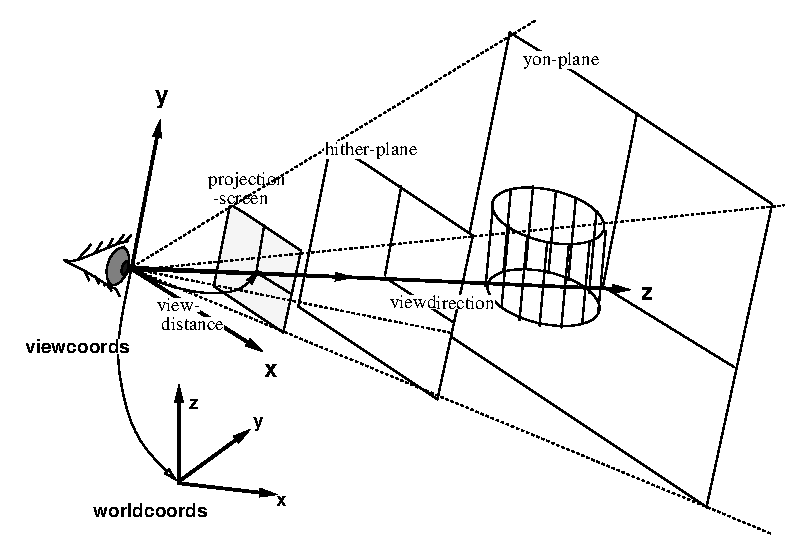
\includegraphics[height=10cm]{fig/viewcoords.ps}
%\epsfile{file=fig/viewcoords.ps,height=10cm}
\end{center}
\caption{viewing座標系と投影画面}
\end{figure}

\begin{refdesc}

\classdesc{viewing}{cascaded-coords}{(viewcoords)}
{viewing変換を定義する。}

\methoddesc{:viewpoint}{}{
この{\bf viewing}の原点のベクトル位置を返す。}

\methoddesc{:view-direction}{}{
{\bf viewing}の原点から画面の中心までのベクトルを返す。
これは、viewing座標系のz軸方向である。}

\methoddesc{:view-up}{}{
ワールド座標系におけるこの{\bf viewing}のy軸ベクトルを返す。
y軸は、{\bf viewport}の上方である。}
\methoddesc{:view-right}{}{
ワールド座標系におけるこの{\bf viewing}のx軸ベクトルを返す。
x軸は、{\bf viewport}の水平右方向である。}

\methoddesc{:look}{from \&optional (to \#f(0 0 0))}{
{\bf :look}は、その目が{\em from}に位置されており、{\em to}の位置を
見ているとしてviewing座標系を設定する。}

% \metdesc{:makeviewcoords}{ ax ay az vpoint}
\longdescription{:init}{
%\&key  \= :target \hspace{12mm} \=  \#f(0 0 0) \hspace{85mm} [メソッド]\\
\&key  \= :target \hspace{12mm} \=  \#f(0 0 0) \` [メソッド]\\
       \> :view-direction \> nil \\
       \> :view-up \>  \#f(0.0 0.0 1.0)) \\
       \> :view-right \>  nil \\
       \> \&allow-other-keys}{
{\bf viewing}は、{\bf cascaded-coords}を継承するので、{\em :pos}や{\em :rot}や{\em :euler}
や{\em :rpy}などの{\em :init}のパラメータはすべてviewing座標系の位置や姿勢を
指定することに使用できる。
しかしながら、viewingの{\em :init}は回転を決定する簡単な方法を持っている。
もし、{\em :target}だけが与えられたとき、視線方向は視点から{\em target}位置
の方向に決定され、{\em :view-right}ベクトルはワールド座標系のxy平面に平行な
x軸に決定される。
{\em :view-direction}を{\em :target}の代わりに指定しても同じ様な
効果を得られる。
もし、{\em :view-up}または{\em :view-right}パラメータを{\em :target}あるいは
{\em :view-direction}に加えて指定するならば、3つの回転パラメータをすべて
自分自身で決定することができる。}

\end{refdesc}

\subsection{投影}

{\bf parallel-projection}と{\bf perspective-projection}クラスは、
投影変換を処理する。この変換は4X4の行列で表現される。すなわち、変換は
3次元の同次座標系で与えられる。
{\bf projection}クラスは、両方のクラスの抽象クラスである。
これらの投影クラスは、viewingクラスを継承しているので、
2つの座標変換(ワールド座標からviewing座標系への変換と投影変換)を
同時に実行することができる。
3Dベクトルと{\tt :project3}メッセージを投影オブジェクトに送ることにより、
4要素の実数ベクトル返す。
{\bf homo2normal}関数は、この同次ベクトルを標準のベクトル表現に変換
するために使用される。
その結果は、標準デバイス座標系(NDC)と呼ばれる座標系上に表現される
ベクトルである。
その中で、見えるベクトルはそれぞれのx,y,z次元において-1から1までの
範囲で表される。
ロボット世界の本当のカメラをシミュレートするために、
{\bf perspective-projection}は{\bf parallel-projection}よりも多く使用される。
{\bf perspective-projection}は、定義されているパラメータが少し多い。
{\tt screenx}と{\tt screeny}は、見える物体が投影されるviewing平面の上のwindowの大きさで、
大きな画面と広い空間が投影される。
{\tt viewdistance}は、視点とview平面との距離を定義しているが、
視角にも関係する。
{\tt viewdistance}を大きくすると、view平面のwindowに狭い範囲が投影される。
{\tt hither}と{\tt yon}パラメータは、クリップする平面の前面と後面の距離を
定義する。
これら2つの平面の外側に位置するオブジェクトは、クリップから除外される。
実際に、このクリップ処理は{\bf viewport}オブジェクトによって実現されている。

\begin{refdesc}

\classdesc{projection}{viewing}
{(screenx screeny hither yon projection-matrix)}
{4x4行列であらわされる投影変換を定義する。}

\methoddesc{:projection}{\&optional pmat}{
もし、{\em pmat}が与えられたならば、
{\tt projection-matrix}のスロットに設定する。
{\bf :projection}は、現在の4x4投影行列を返す。}
\methoddesc{:project}{vec}{
{\em vec}は、4要素を持つ3次元同次ベクトルである。
{\em vec}は、投影行列により変換される。
そして、変換された結果である同次表現が返される。}
\methoddesc{:project3}{vec}{
{\em vec}は、標準の3Dベクトル。
{\em vec}は、投影行列により同次化され変換される。
そして、変換された結果である同次表現が返される。}
\methoddesc{:view}{ vec}{
{\em vec}にviewing変換と投影変換を連続的に適用する。
そして、変換された結果である同次表現が返される。}
\methoddesc{:screen}{xsize (\&optional (ysize xsize))}{
viewing画面の大きさを変える。
大きくすると、広いviewが得られる。}
\methoddesc{:hither}{ depth-to-front-clip-plane}{
視点からクリップ前面までの距離を決定する。
このクリップ前面よりも前にあるオブジェクトはクリップから除外される。}
\methoddesc{:yon}{ depth-to-back-clip-plane}{
視点からクリップ後面までの距離を変える。
このクリップ後面よりも後ろにあるオブジェクトはクリップから除外される。}
\methoddesc{:aspect}{\&oiptional ratio}{
アスペクト比は、screen-yとscreen-xとの比である。
もし、{\em ratio}が与えられたならば、
アスペクト比は変えられ、screen-yはscreen-x * {\em ratio}に設定される。
{\bf :aspect}は、現在のアスペクト比を返す。}
\longdescription{:init}{
%\&key \= :hither  \hspace{5mm} \= 100.0 \hspace{100mm}[メソッド]\\
\&key \= :hither  \hspace{5mm} \= 100.0 \` [メソッド]\\
      \> :yon    \> 1000.0 \\
      \> :aspect \> 1.0  \\
      \> :screen \> 100.0 \\
      \> :screen-x  \> screen \\
      \> :screen-y \> (* screen-x aspect) \\
      \>  \&allow-other-keys}{
{\bf viewing}と{\bf projection}を初期化する。}

\vspace{5mm}

\classdesc{parallel-viewing}{projection}{()}{
平行投影を定義する。
{\bf hid}(陰線消去関数)は平行投影では扱うことが出来ない。}

\metdesc{:make-projection}{}

\classdesc{perspective-viewing}{projection}
{(viewdistance)}{透視投影変換を定義する。}

\metdesc{:make-projection}{ }
\methoddesc{:ray}{u v}{
視点から正規化画面の上にある{\em (u,v)}への単位方向ベクトルを返す。}
\methoddesc{:viewdistance}{\&optional vd}{
{\tt viewdistance}は、視点から画面迄の距離である。
もし、{\em vd}が与えられたならば、{\tt viewdistance}に設定される。
{\tt viewdistance}は、カメラの焦点距離と一致する。
{\em vd}を大きくすれば、ズームアップされたviewを得ることができる。
{\bf :viewdistance}は、現在の{\tt viewdistance}を返す。}
\methoddesc{:view-angle}{\&optional ang}{
画面の対角線を見込む角度が{\em ang}ラジアンであるように画面の大きさを設定する。
20度(約0.4ラジアン)から50度(約0.9ラジアン)までの角度が自然な透視view
を生成することができる。
角度を大きくすると歪んだviewを生成する。
そして、狭くすると直角(平行)viewingのような平坦なviewが生成される。
{\bf :view-angle}は、現在の視角あるいは新しい視角をラジアンで返す。}
\methoddesc{:zoom}{\&optional scale}{
もし、{\em scale}が与えられたならば、画面は{\em scale}によって
現在の大きさを相対的に変化させる({\tt viewdistance}は変化しない)。
もし、{\em scale}に0.5を与えるならば、以前のviewより2倍広いviewを得られる。
{\bf :zoom}は、新しい視角をラジアンで返す。}
\methoddesc{:lookaround}{alfa beta}{
視点を移動し回転させる。
回転中心は、視線の上で{\tt hither}平面と{\tt yon}平面の中間点
に与えられる。
viewing座標系は、ワールド座標系のz軸回りに{\em alfa}ラジアン回転し、
ローカル座標系のx軸回りに{\em beta}ラジアン回転される。
{\bf :lookaround}は、{\bf viewing}の中心にあるオブジェクト回りに視線を
動かすことができる。}
\methoddesc{:look-body}{bodies}{
視線、画面の大きさおよびhither/yonをすべての{\em bodies}に適合するviewport
となるよう変える。視点は変化しない。
視線は、すべての{\em bodies}のbounding boxの中心を通る視線から選択される。}

\metdesc{:init}{ \&key (:viewdistance 100.0) \&allow-other-keys}

\end{refdesc}

\subsection{Viewport}

{\bf viewport}クラスは、正規デバイス座標系(NDC)の中の3次元viewportのクリップ
を実行する。そして、デバイスに依存する座標系に結果を作る。
{\bf viewport}は、画面上の見える四角領域の境界表現である。
{\bf viewport}の物理的な大きさ(x軸とy軸方向のドット数)は、
{\bf :init}メッセージの中の{\em :width}と{\em :height}との引き数
で与えられなければならない。
{\em :xcenter}と{\em :ycenter}引き数は、viewportの物理的な位置を決定する。
画面の原点からのそれぞれの次元が絶対的に与えられているテクトロニクス4014
のような基本的なディスプレイデバイスを使っているとき、これら2つのパラメータは、実際に画面の上にオブジェクトを描く位置を決定する。
もし、位置が親windowから相対的に決まるXwindowのような精巧なディスプレイ
デバイスを使っているなら、
viewportを動かすためにviewportのパラメータを変える必要はない。
なぜなら、これらのパラメータは、実際のディスプレイ位置に依存しないからである。。

{\bf viewport}クラスは、四角領域の左下をviewportの原点と仮定している。
そして、y軸は上方向に伸びているとする。
しかし、多くのwindowシステムやディスプレイデバイスでは原点を左上とし、
y軸が下方向に伸びているとしている。
この問題を回避するために、{\em :height}パラメータに負の値を与えればよい。

\begin{refdesc}

\funcdesc{homo-viewport-clip}{v1 v2}{
{\em v1}と{\em v2}は、4要素を持つ同次ベクトルであって、
3次元空間の線分として表現される。
その線分は、$x=-1, x=1, y=-1, y=1, z=0, z=1$の境界でクリップされる。
そして、2つのベクトルのリストを返す。
もし、その線分が{\bf viewport}の外側に完全に置かれているならば、
NILを返す。}

\classdesc{viewport}{coordinates}{}
{viewport変換は、デバイスで指定される座標系にNDC(正規化デバイス座標系)を作る。
{\bf coordinates}クラスを継承しているため、{\bf viewport}はサイズと投影画面の
相対位置を定義している。}

\methoddesc{:xcenter}{\&optional xcenter}{
この{\bf viewport}のx軸の中心を返す。
もし、{\em xcenter}が与えられていれば、設定を行う。}
\methoddesc{:ycenter}{\&optional ycenter}{
この{\bf viewport}のy軸の中心を返す。}
\methoddesc{:size}{\&optional size}{
この{\bf viewport}のx軸とy軸方向の大きさのリストを返す。}

\methoddesc{:width}{ \&optional width}{この{\bf viewport}の幅を{\em width}に
設定する。}
\methoddesc{:height}{ \&optional height}{この{\bf viewport}の高さを
{\em height}に設定する。}
\methoddesc{:screen-point-to-ndc}{p}{
{\em p}は、物理的画面の中の位置を表現する実数ベクトルである。
{\em p}は、正規化デバイス座標系(NDC)の中での表現に変換される。}
\methoddesc{:ndc-point-to-screen}{p}{
この{\bf viewport}のNDC表現である{\em p}を画面の物理的位置に変換する。}
\methoddesc{:ndc-line-to-screen}{p1 p2 \&optional (do-clip t)}{
2つの3次元ベクトル{\em p1}と{\em p2}は、NDCの中の線分を定義する。
これらの2つの端点は、画面空間の表現に変換される。
もし、{\em do-clip}がnon-NILなら、その線分はクリップされる。}
\methoddesc{:init}{\&key (:xcenter 100) (:ycenter 100) (:size 100)
(width 100) (height 100)}
{新しい{\bf viewport}オブジェクトを作る。}

\end{refdesc}

\subsection{Viewer}
画面の上に描画するためには、4つのオブジェクトが必要である。
1つは描かれたオブジェクト、2つはviewing座標系と投影で定義される{\bf viewing}、
3つはNDCの中でのクリップ処理のための{\bf viewport}とNDCから物理的画面座標系への
変換、4つは
物理的ディスプレイデバイスの上に描画関数を実行する{\bf viewsurface}。
{\bf viewer}オブジェクトは、{\bf viewing}と{\bf viewport}と{\bf viewsurface}
オブジェクトを持ち、
座標系変換を連続的に制御する。
\ref{Drawings}節に記述される{\bf draw}と{\bf hid}関数は{\bf viewer}の
インスタンスを使用する。

\begin{refdesc}

\classdesc{viewer}{object}
{(eye :type viewint) \\
\> (port :type viewport) \\
\> (surface :type viewsurface)} 
{viewingからviewportを経由してviewsurfaceへ移るCascaded Coordinatesの変換を定義する。}

\methoddesc{:viewing}{\&rest msg}{
もし、{\em msg}が与えられたならば、{\em msg}は{\bf viewing}{\tt (eye)}オブジェクト
に送られる。そうでなければ、{\bf viewing}{\tt (eye)}オブジェクトが返される。}
\methoddesc{:viewport}{\&rest msg}{
もし、{\em msg}が与えられたならば、{\em msg}は{\bf viewport}{\tt (port)}オブジェクト
に送られる。そうでなければ、{\bf viewport}{\tt (port)}オブジェクトが返される。}
\methoddesc{:viewsurface}{\&rest msg}{
もし、{\em msg}が与えられたならば、{\em msg}は{\bf viewsurface}{\tt (surface)}オブジェクト
に送られる。そうでなければ、{\bf viewsurface}{\tt (surface)}オブジェクトが返される。}
\methoddesc{:adjust-viewport}{}{
{\bf viewsurface}の大きさが変えられたとき、{\bf :adjust-viewport}は
{\tt port}に固有のメッセージを送ることにより{\bf viewport}の変換を変える。}
\methoddesc{:resize}{width height}{
{\bf viewsurface}に{\tt :resize}メッセージを送り、{\bf viewport}に{\tt :size}メッセージを送る
ことによりviewsurfaceの大きさを変える。}
\methoddesc{:draw-line-ndc}{ p1 p2 \&optional (do-clip t)}{
NDCの中に定義される2つの端点{\em p1,p2}を結ぶ線を描く。}
\methoddesc{:draw-polyline-ndc}{polylines \&optional color}{
NDCの中に定義される端点を結ぶ多角形を描く。}
\methoddesc{:draw-star-ndc}{center \&optional (size 0.01) color}{
NDCの中に十字マークを描く。}
\methoddesc{:draw-box-ndc}{low-left up-right \&optional color}{
NDCの中に四角形を描く。}
\methoddesc{:draw-arc-ndc}{point width height angle1 angle2 \&optional color}{
NDCの中に円弧を描く。
この{\bf viewer}に結び付く{\bf viewsurface}オブジェクトは、{\bf :arc}メッセージを
受けなければならない。}
\methoddesc{:draw-fill-arc-ndc}{ point width height angle1 angle2 \&optional color}{
NDCの中に塗り潰し円弧を描く。}
\methoddesc{:draw-string-ndc}{position string \&optional color}{
NDCの中に定義される{\em position}に{\em string}を描く。}
\metdesc{:draw-image-string-ndc}{position string \&optional color}
\metdesc{:draw-rectangle-ndc}{position width height \&optional color}
\metdesc{:draw-fill-rectangle-ndc}{point width height \&optional color}
\methoddesc{:draw-line}{p1 p2 \&optional (do-clip t)}{
ワールド座標系に定義される2つの端点{\em p1,p2}を結ぶ線を描く。}
\methoddesc{:draw-star}{position \&optional (size 0.01) color}{
ワールド座標系の{\em position}位置に十字マークを描く。}
\methoddesc{:draw-polyline}{vlist \&optional color}{
ワールド座標系の{\em vlist}端点を結ぶ多角形を描く。}
\methoddesc{:draw-box}{center \&optional (size 0.01)}{
ワールド座標系の{\em center}に四角形を描く。}
\methoddesc{:draw-arrow}{p1 p2}{
{\em p1}から{\em p2}へ向けての矢印を描く。}
\metdesc{:draw-edge}{edge}
\metdesc{:draw-edge-image}{edge-image}
\metdesc{:draw-faces}{face-list \&optional (normal-clip nil)}
\metdesc{:draw-body}{body \&optional (normal-clip nil)}
\methoddesc{:draw-axis}{coordinates \&optional size}{
{\em coordinates}で定義される軸を{\em size}の長さで描く。}
\methoddesc{:draw}{\&rest things}{
3次元の幾何学オブジェクトを描く。
もし、オブジェクトが3次元ベクトルならば、その位置に小さな十字マークを描く。
もし、3次元ベクトルのリストであれば、多角形を描く。
もし、{\em thing}が{\tt :draw}メッセージを受けたならば、
この{\bf viewer}を引き数としてそのメソッドが呼び出される。
もし、オブジェクトが{\tt :drawners}メソッドを定義しているならば、
{\bf :draw}メッセージは{\tt :drawners}の結果に送られる。
{\tt line, edge, polygon, face}および{\tt body}オブジェクトは、
{\bf viewer}に定義されている{\bf :draw-xxx}(xxxにそのオブジェクトのクラス名が入る)
メソッドによって描かれる。}
\methoddesc{:erase}{\&rest things}{
背景色で{\em things}を描く。}
\methoddesc{:init}{\&key :viewing :viewport :viewsurface}{
{\em viewing, viewport}および{\em viewsurface}をこの{\bf viewer}のスロット
{\tt eye, port}と{\tt surface}に設定する。}

\longdescription{view}{\&key \= (:size 500) (:width size) (:height size)
\` [関数] \\
%\hspace{74mm} [関数] \\
\> (:x 100) (:y 100) \\
\> (:title "eusx") \\
\> (:border-width 3) \\
\> (:background 0) \\
\> (:viewpoint \#f(300 200 100)) (:target \#f(0 0 0)) \\
\> (:viewdistance 5.0)  (:hither 100.0) (:yon 10000.0) \\
\> (:screen 1.0) (:screen-x screen) (:screen-y screen) \\
\> (:xcenter 500) (:ycenter 400) \\}
{新しい{\bf viewer}を作り、{\bf *viewer*}リストに置く。}

\end{refdesc}

\newpage
\subsection{\label{Drawings}描画}

\begin{refdesc}

\funcdesc{draw}{[viewer] \&rest thing}{
{\em viewer}に{\em thing}を描く。
{\em thing}は、座標系、立体、面、エッジ、ベクトル、2つのベクトルのリストのどれでも可能である。
{\tt (progn (view) (draw (make-cube 10 20 30)))}
は、xwindowに立方体を描く。}


\funcdesc{draw-axis}{[viewer] [size] \&rest thing}{
{\em viewer}の中に{\em thing}の座標系の軸を{\em size}の長さで描く。
{\em thing}は、座標系から得られるどのオブジェクトでも可能である。}

\funcdesc{draw-arrow}{p1 p2}{
{\bf *viewer*}に{\em p1}から{\em p2}に向かう矢印を描く。}

\funcdesc{hid}{[viewer] \&rest thing }
{{\em viewer}に陰線処理された画像を描く。
{\em thing}は、{\tt face}または{\tt body}が可能である。}

\funcdesc{hidd}{[viewer] \&rest thing }{
陰線を点線で描くことを除いて、{\bf hid}と同じである。}

\funcdesc{hid2}{body-list viewing}{
edge-imageオブジェクトで表現される陰線処理画像を生成する。
その結果は{\bf *hid*}に置かれる。}

\longdescription{render}{\&key \= :bodies :faces (:viewer *viewer*) \` [関数]\\
\> (:lights *light-sources*)\\
\> (colormap *render-colormap*) (y 1.0)}{
{\em bodies}と{\em faces}にレイトレーシングを行い、陰面消去した画像を生成する。
{\bf viewing, viewport}および{\bf viewsurfaceは}、{\em viewer}から得られる。
{\em lights}は、{\tt light-source}(光源)オブジェクトのリストである。
{\em colormap}は、Xwindowの{\bf colormap}オブジェクトである。
それぞれの{\em bodies}と{\em faces}は、割り当てられるカラー属性を
持たなければならない。
{\em colormap}に定義されているカラーLUTの名前を{\tt :color}メッセージで
送ることによりカラー属性を設定できる。
一般にこの関数は、Xlib環境下でのみ働く。
{\tt demo/renderdemo.l}のサンプルプログラムを見ること。}

\funcdesc{make-light-source}{pos \&optional (intensity 1.0)}{
{\em pos}の位置に光源オブジェクトを作る。
{\em intensity}は、デフォルトの光の強さを増す拡大比である。
もっと正確に強さを決定するためには、光源の{\tt :intensity}メソッドを
使用する。}

\macrodesc{tektro}{file \&rest forms}{
{\tt *tektro-port*}ストリームのために{\em file}をオープンし、
{\em forms}を評価する。
これは、tektro描画の出力を直接{\em file}に書き込むために使用される。}

\macrodesc{kdraw}{file \&rest forms}{
{\bf kdraw}は、{\tt kdraw}または{\tt idraw}で読み込めるポストスクリプトファイルを
生成するためのマクロ命令である。
{\bf kdraw}は、{\tt :output}モードで{\em file}をオープンし、
{\tt *viewer*}を置き換えるためのkdraw-viewsurfaceとviewportを
作り、{\em forms}を評価する。
それぞれの{\em forms}は、{\tt draw}や{\tt hid}のような描画関数の
どれかを呼び出す。
これらの{\em forms}からの描画メッセージは、{\tt kdraw-viewsurface}に
直接出力される。この出力は{\tt idraw}や{\tt kdraw}で認識できる
ポストスクリプト表現にメッセージを変換する。
そして、{\em file}に蓄積する。
{\tt idraw}または{\tt kdraw}が呼び出され{\em file}がオープンされたとき、
EusViewer windowに書いたものと同一の図形を見ることができる。
その図形は、{\tt idraw}の機能で変更することができる。
そして、最終描画は{\tt epsfile}環境を用いることにより\LaTeX ドキュメント
に組み込むことができる。
この機能は、"llib/kdraw.l"のファイルに記述されている。}

\macrodesc{pictdraw}{file \&rest forms}{
{\bf pictdraw}は、MacintoshのPICTフォーマットで画像ファイルを
生成するためのマクロである。
{\bf pictdraw}は、{\em file}を{\tt :output}モードでオープンし、
pictdraw-viewsurfaceを作り、{\tt *viewer*}のviewportに置き換え、
{\em forms}を評価する。
{\em forms}は、それぞれ{\tt draw}あるいは{\tt hid}のような描画関数のどれかを
呼び出すものである。
これらの書式からの描画メッセージは、{\tt kdraw-viewsurface}に
直接出力された後、PICTフォーマットへのメッセージに変換され,
{\em file}へ蓄積される。
このPICTフォーマットは、Macintoshの{\tt macdraw}や{\tt teachtext}で
認識することができる。}

\funcdesc{hls2rgb}{hue lightness saturation \&optional (range 255)}{
HLS(Hue, Lightness, Saturation)で表現される色を、RGB表現に変換する。
HLSは、しばしばHSLとして参照される。
{\em hue}は、rainbow circle(0から360)の色で表現される。
0が赤で45が黄で120が緑で240が青で270が紫そして360が再び赤となる。
{\em lightness}は、0.0から0.1の値を持ち、黒から白までの明るさを表現する。
{\em lightness}が0のときは、{\em hue}や{\em saturation}にかかわらず
黒となる。そして、{\em lightness}が1のときは、白となる。
{\em saturation}は、0.0から1.0までの値を持ち、色の強さを表現する。
{\em saturation}の値が大きいと鮮明な色調を生成し、小さい値は弱く濁った色調
を生成する。
{\em range}は、RGB値の限界を示す。
もし、それぞれの色に8ビットの値が割り当てられているカラーディスプレイ
を使っているならば、{\em range}は255とすべきである。
もし、RGBに16ビットの整数が仮想的に割り当てられているXwindowを使って
いるならば、{\em range}は65536とすべきである。
HSVとHLSとの違いに注意すること。
HLSでは、鮮明な(rainbow)色は{\tt lightness=0.5}で定義されている。}
\funcdesc{rgb2hls}{red green blue \&optional (range 255)}{
RGBの色表現を、HLS表現に変換する。}

\end{refdesc}

\subsection{アニメーション}
\index{animation}
EusLispのアニメーションは、グラフィックアクセラレータを持たない
普通のワークステーション上での擬似リアルタイムグラフィックス機能を備えている。
その基本的な考え方は、長い時間かかって生成された1連の画像を高速に
再表示することである。
画像は2つの方法で保存される。
1つは、完全なピクセル画像を持つたくさんのXwindow pixmapを保存する。
もう1つは、陰線処理で得られる線分データを保存する。
前者は、高速で陰面処理された画像を表示するための方法であるが、
長いアニメーションではたくさんのメモリーをX serverに要求するため
適さない。
後者は、メモリーが少なくて済み、データをディスクに蓄積するのに適する。
しかし、線分の数が増加したならば、性能を悪化させる。

他の方法として、描かれるオブジェクトの構成を得て、
{\bf *viewer*}に描画を生成する関数をユーザーが作ることもできる。
{\bf pixmap-animation}は、{\em count}引数で指定された数と同じ回数この関数を呼び出す。
それぞれの呼び出し後、Xwindowと仮定される{\tt viewsurface}の内容は、
新しく作られたXwindow pixmapにコピーされる。
これらのpixmapは、{\bf playback-pixmap}で再表示される。
同様に、{\bf hid-lines-animation}は{\bf hid}の結果から見える線分を抜き出し、
リストに蓄積する。
そのリストは、{\bf playback-hid-lines}によって再表示される。

以下に示す関数は、"llib/animation.l"に定義されており、
"llib/animdemo.l"の中にはETA3 マニピュレータのモデルに関して
{\bf hid-lines-animation}を用いたアニメーションの
サンプルプログラムを含んでいる。

\begin{refdesc}
\macrodesc{pixmap-animation}{count \&rest forms}{
{\em forms}は、{\em count}回評価される。
それぞれの評価後、{\tt *viewsurface*}の内容は新しいpixmapにコピーされる。
{\em count}枚の{\bf pixmap}のリストが、返される。}
\funcdesc{playback-pixmaps}{pixmaps \&optional (surf *viewsurface*)}{
{\em pixmaps}リストのなかの{\bf pixmap}はそれぞれ、
%{\em wait}$\mu$秒の間隔をおいて
{\em surf}に連続的にコピーされる。}

\macrodesc{hid-lines-animation}{count \&rest forms}{
{\bf hid}への呼び出しを含む{\em forms}が{\em count}回評価される。
それぞれの評価後、{\bf *hid*}が持つ{\bf hid}の結果は検索され、
見える線分は2点一組のリストの形で集められる。
{\em count}長さのリストが返される。}
\funcdesc{playback-hid-lines}{lines \&optional (view *viewer*)}{
{\em lines}は、2点一組のリストである。
{\em view}の上に線分を連続的に描く。
他のpixmapを割り当てるときにフリッカーフリーアニメーションを生成するために
2重バッファ技法が使用される。}

\funcdesc{list-visible-segments}{hid-result}{
{\em hid-result}のedge画像のリストから見える線分を集める。}

\end{refdesc}

\newpage

\section{Xwindow インターフェース}
\markright{\arabic{section}. Xwindow}
Euslisp上のXwindowインターフェースは、{\tt 'eusx'}という
名前でEuslispが呼び出されたとき、実行可能となる。
\footnote{eusxは、eusへのシンボリックリンクである。}
eusxは、起動時に環境変数"DISPLAY"を参照してXserverに接続を試みるため、
自分のXseverに環境変数"DISPLAY"が正しく設定されていなければならない。

Euslispには、次の3つのレベルのXwindowインターフェースが定義されている。
(1) Xlib関数, (2) Xlibクラスと(3) XToolKitクラスである。
この節と次のXToolKitの節に記述されている
全てのXwindow関数は、"X"パッケージの中に含まれている。
それらの関数名は、元のXlib関数名から最初の"X"を省いき、全ての文字を大文字に
変更したものとなっている。
例えば{\tt XdefaultGC}は{\tt X:DEFAULTGC}と名付けられていて、
{\tt X:XDEFAULTGC}ではない。

Xlib関数は、Xwindowシステムへの低レベルインターフェースで、
foreign関数として定義されている。
これらのXlib関数は、パラメータの型チェックあるいは
パラメータの数のチェックを実行していないため、
十分注意して使用しなければならない。
例えば、すべてのXlibの呼び出しにおいてXserverとの接続を確認するために
{\tt x:*display*}を引き数として要求する。もし、指定し忘れたならば、Xlibは
エラーを通知し、そのプロセスは死ぬ。
このような不便を避け、オブジェクト指向のインターフェースを作るために、
2番めのレベルのインターフェースであるXlibクラスが備わっている。
%By instantiating the xwindow class, you will get a window on a screen,
%and sending messages to the instance, you can draw lines, strings, or whatever
%in it.
この節では、この2番めのレベルのインターフェースに焦点を当てる。
XToolKitと呼ばれるもっと高レベルのXwindowライブラリは、次節で
説明されている。

この節に記述されているクラスは、以下の継承の階層を持っている。

\begin{quote}
\begin{verbatim}
propertied-object
   viewsurface
      x:xobject
         x:gcontext
         x:xdrawable
             x:xpixmap
             x:xwindow
   colormap
\end{verbatim}
\end{quote}

\subsection{\label{xvariables}Xlibのグローバル変数とその他関数}
\begin{refdesc}
\vardesc{x:*display*}{Xのdisplay ID(整数)}
\vardesc{x:*root*}{デフォルトのroot windowオブジェクト}
\vardesc{x:*screen*}{デフォルトのscreen ID(整数)}
\vardesc{x:*visual*}{デフォルトのvisual ID(整数)}
\vardesc{x:*blackpixel*}{黒色のpixel値 = 1}
\vardesc{x:*whitepixel*}{白色のpixel値 = 0}
\vardesc{x:*fg-pixel*}{window作成時に参照されるデフォルトの文字色のpixel値、ふつう{\tt *blackpixel*}。}
\vardesc{x:*bg-pixel*}{window作成時に参照される背景色のpixel値、ふつう{\tt *whitepixel}。}
\vardesc{x:*color-map*}{システムのデフォルトカラーマップ}
\vardesc{x:*defaultGC*}{pixmap生成時に参照されるデフォルトgcontext}
\vardesc{x:*whitegc*}{文字色が白色のgcontext}
\vardesc{x:*blackgc*}{文字色が黒色のgcontext}
% \vardesc{*gray-gc*}{ハーフトーンのGC}
\vardesc{*gray-pixmap*}{{\tt (make-gray-pixmap 0.5)}の結果。}
\vardesc{*gray25-pixmap*}{
1/4のピクセルが{\tt *fg-pixel*}であり、3/4が{\tt *bg-pixel*}である16x16のpixmap。}
\vardesc{*gray50-pixmap*}{1/2のピクセルが{\tt *fg-pixel*}である16x16のpixmap。}
\vardesc{*gray75-pixmap*}{3/4のピクセルが黒色である16x16のpixmap。}
\vardesc{*gray25-gc*}{{\tt *gray25-pixmap*}から作る25\%のグレーGC。}
\vardesc{*gray50-gc*}{{\tt *gray50-pixmap*}から作る50\%のグレーGC。}
\vardesc{*gray75-gc*}{{\tt *gray75-pixmap*}から作る75\%のグレーGC。}
\vardesc{*gray*}{{\tt "\#b0b0b0"}}
\vardesc{*bisque1*}{{\tt "\#ffe4c4"}}
\vardesc{*bisque2*}{{\tt "\#eed5b7"}}
\vardesc{*bisque3*}{{\tt "\#cdb79e"}}
\vardesc{*lightblue2*}{{\tt "\#b2dfee"}}
\vardesc{*lightpink1*}{{\tt "\#ffaeb9"}}
\vardesc{*maroon*}{{\tt "\#b03060"}}
\vardesc{*max-intensity*}{65535}
\vardesc{font-cour8}{{\tt (font-id "*-courier-medium-r-*-8-*")}}
\vardesc{font-cour10}{{\tt (font-id "*-courier-medium-r-*-10-*")}}
\vardesc{font-cour12}{{\tt (font-id "*-courier-medium-r-*-12-*")}}
\vardesc{font-cour14}{{\tt (font-id "*-courier-medium-r-*-14-*")}}
\vardesc{font-cour18}{{\tt (font-id "*-courier-medium-r-*-18-*")}}
\vardesc{font-courb12}{{\tt (font-id "*-courier-bold-r-*-12-*")}}
\vardesc{font-courb14}{{\tt (font-id "*-courier-bold-r-*-14-*")}}
\vardesc{font-courb18}{{\tt (font-id "*-courier-bold-r-*-18-*")}}
\vardesc{font-helvetica-12}{{\tt (font-id "*-Helvetica-Medium-R-Normal-*-12-*")}}
\vardesc{font-lucidasans-bold-12}{{\tt (font-id "lucidasans-bold-12")}}
\vardesc{font-lucidasans-bold-14}{{\tt (font-id "lucidasans-bold-14")}}
\vardesc{font-helvetica-bold-12}{{\tt (font-id "*-Helvetica-Bold-R-Normal-*-12-"
)}}
\vardesc{font-a14}{{\tt (font-id "*-fixed-medium-r-normal-*-14-*")}}

%\vardesc{x:*reversevideo*}{}
\vardesc{x:*xwindows*}{Euslispによる子windowを含んだ全てのwindowのリストを
保持する。}
\vardesc{x:*xwindow-hash-tab*}{drawable IDからxwindowオブジェクトを
探すためのハッシュテーブル。
{\tt x:nextevent}で得られるイベント構造はwindow IDであるため、
{\tt x:window-main-loop}はこのテーブルを使用して一致するxwindowオブジェクト
を知るために{\tt x:event-window}を呼び出す。}
%\vardesc{x:gcval}{}

\funcdesc{xflush}{}{
Xlibのコマンドバッファに保有するコマンドをすべてXserverに送る。
XlibバッファがXserverに出力するため、
Xserverに発行されたコマンドは、すぐに実行されない。
これは、ネットワークの渋滞およびプロセスの切替え頻度を減少させるために
必要である。
コマンドの効果を見るためにコマンドバッファを掃き出す方法として、
{\bf xflush}を使用するかあるいは{\bf :flush}メッセージをxwindowオブジェクトに
送る。}

\end{refdesc}

\subsection{Xwindow}

\begin{refdesc}

\classdesc{Xobject}{geometry:viewsurface}{}{
すべてのXwindowに関連するクラスの共通のスーパークラスである。
現在、スロットもメソッドも定義されていない。}

\classdesc{Xdrawable}{Xobject}
{(drawable  \hspace{10mm} \=  ; drawable  ID \\
 \> gcon \>  ; this drawable's default graphic context object\\
\> bg-color \> ; background color \\
\> width height \> ; horizontal and vertical dimensions in dots}
{{\bf Xdrawable}は、線分や文字列のようなグラフィックオブジェクト
を描くための四角領域を定義する。
{\bf Xdrawable}は、xwindowやxpixmapのための共通メソッド
を定義するための抽象クラスであり、
このクラスのインスタンスは何の効果も持っていない。}

\methoddesc{:init}{id}{
{\em id}は、このdrawableのIDとして{\tt drawable}スロットに設定される。
新しいGC(graphic context)が生成され、このdrawableオブジェクトの
デフォルトGCとして{\tt gcon}に設定される。}
\methoddesc{:drawable}{}{drawable IDを返す。}
\methoddesc{:flush}{}{Xlibのバッファに保有されるコマンドを掃き出す。}
\methoddesc{:geometry}{}{
7つの幾何学属性のリストを返す。
そのリストは、root-window-id, x座標, y座標,
幅, 高さ, 枠線の幅, visualの深さである。}

\methoddesc{:height}{}{
この{\bf Xdrawable}の高さ(y軸方向のドット数)を返す。}
\methoddesc{:width}{}{
この{\bf Xdrawable}の幅(x軸方向のドット数)を返す。}
\methoddesc{:gc}{\&rest newgc}{
もし、{\em newgc}が与えられない場合、現在のGCオブジェクトを返す。
もし、{\em newgc}が{\bf gcontext}のインスタンスなら、
この{\bf Xdrawable}の{\tt gc}に設定する。
そうでなければ、{\em newgc}はメッセージとみなされ、
現在の{\tt gc}に送られる。}
\methoddesc{:pos}{}{
この{\bf Xdrawable}の位置を示す整数ベクトルを返す。
位置は親windowの相対位置としていつも定義され、
windowマネージャの仲介のもとにルートwindowの直接の子windowとして
生成されたwindowは、ルートwindowの本当の位置に関わらず、環境の
タイトルwindowの固定座標を返す。}
\methoddesc{:x}{}{この{\bf Xdrawable}の親windowとの相対的な現在のx座標を返す。}
\methoddesc{:y}{}{この{\bf Xdrawable}の親windowとの相対的な現在のy座標を返す。}
\methoddesc{:copy-from}{drw}{
{\em drw}は、他の{\bf drawable}オブジェクト(Xwindowまたはpixmap)である。
{\em drw}の内容がこの{\bf Xdrawable}にコピーされる。}

\begin{figure}
\begin{center}
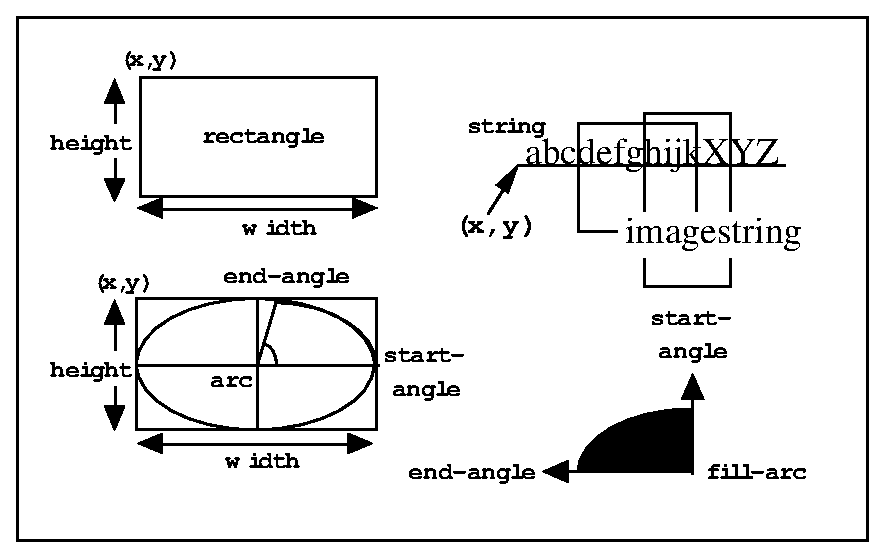
\includegraphics[height=6cm]{fig/xdraw.ps}
%\epsfile{file=fig/xdraw.ps,height=6cm}
\end{center}
\caption{描画の基本\label{xdraw}}
\end{figure}


\methoddesc{:point}{x y \&optional (gc gccon)}{
$(x, y)$の位置にオプションの{\em gc}で点を描く。}
\methoddesc{:line}{x1 y1 x2 y2 \&optional (gc gcon)}{
{\em (x1,y1)}から{\em (x2,y2)}へオプションの{\em gc}を用いて
線分を描く。{\em x1, y1, x2, y2}は整数でなければならない。}
\methoddesc{:rectangle}{x y width height \&optional (gc gcon)}{
{\em (x,y)}を中心として{\em width}の幅と{\em height}の高さを持つ
四角形を描く。}
\methoddesc{:arc}{x y width height angle1 angle2 \&optional (gc gcon)}{
{\em (x,y)}を中心として{\em width}の幅と{\em height}の高さを持つ
四角形に内接する楕円の円弧を描く。{\em angle1}が始まりの角度を示し、
{\em angle2}が終わりの角度を示す。これらの角度の単位はラジアンである。}
\methoddesc{:fill-rectangle}{x y width height \&optional (gc gcon)}{
四角領域を埋める。}
\methoddesc{:fill-arc}{x y width height angle1 angle2 \&optional (gc gcon)}{
円弧の中を埋める。}
\methoddesc{:string}{x y str \&optional (gc gcon)}{
{\em (x,y)}の位置から文字列{\em str}を表示する。背景は、書かない。}
\methoddesc{:image-string}{x y str \&optional (gc gcon)}{
文字列{\em str}を表示する。文字列は、背景色で満たされる。}
\methoddesc{:getimage}{\&key :x :y :width :height (:mask \#ffffffff) (:format 2)}{
serverからximageを取り、ピクセルデータを文字列として返す。
serverから送られるピクセルデータは、一端 Xlibのximage構造に蓄積される。
その後、行毎に文字列にコピーされる。
ximage構造は、自動的に破壊される。
{\tt :getimage}により得られた画像文字列は、{\tt pixel-image}を作るために
使用できる。また、\ref{PBMfile}節に書かれているようにpbmフォーマットのファイルに
書き込むことができる。}
\methoddesc{:putimage}{image \&key :src-x :src-y :dst-x :dst-y :width :height ((:gc g) gc)}{
この{\bf Xdrawable}の指定された位置に{\em image}を表示する。
{\em image}は、文字列あるいはximage構造へのアドレスポインターである。}
\methoddesc{:draw-line}{from to}{
{\bf :line}メソッドと同じである。
他の{\bf viewsurface}クラスとの互換性を提供できる。}
\methoddesc{:line-width}{\&optional dots}{
この{\bf Xdrawable}のデフォルトGCの線の幅を設定する。
{\tt :gc :line-width}メッセージの使用を推薦する。}
\methoddesc{:line-style}{\&optional dash}{
この{\bf Xdrawable}のデフォルトGCの線スタイルを設定する。
{\tt :gc :line-style}の使用が好まれる。}
\methoddesc{:color}{\&optional c}{この{\bf Xdrawable}の色を設定する。}
%\methoddesc{:set-show-mode}{}{
%コピーモードを設定する。この関数は、ふつう白黒ディスプレイで使用される。}
%\methoddesc{:set-erase-mode}{}{
%消去モードを設定する。この関数は、ふつう白黒ディスプレイで使用される。}
%\methoddesc{:set-xor-mode}{}{
%反転モードを設定する。この関数は、ふつう白黒ディスプレイで使用される。}
\methoddesc{:clear}{}{
全画面を消去する。この関数は、{\tt :clear-area}を呼び出す。}
\methoddesc{:clear-area}{\&key :x  :y :width :height :gc}{
{\bf :fill-rectangle}メソッドを用いて四角領域を消去する。}

\classdesc{Xpixmap}{Xdrawable}{}{
pixmapは、画像バッファあるいは背景のパターンとしてしばしば用いられる
drawableである。xwindowと異なり、xwindowにコピーされるまで
pixmap自身を見ることはできないし、pixmapはどんなイベントも発生しない。}

\methoddesc{:init}{id}{このpixmapを初期化する。}
\methoddesc{:create}{\&key (:width 500) (:height 500) (:depth 1) (:gc *defaultgc*)}{
デフォルトGCとして{\em :gc}を持つ、{\em width}$\times${\em height}のpixmapを作成する。}
\methoddesc{:create-from-bitmap-file}{fname}{
{\em file}で指定されるbitmapファイルからpixmapを作る。}
\methoddesc{:write-to-bitmap-file}{fname}{
このpixmapの内容を{\em fname}で指定されるbitmapファイルに書き込む。
このファイルは、{\bf :create-from-bitmap-file}メソッドで
pixmapを作り、読み戻すことができる。}
\methoddesc{:destroy}{}{
このpixmapを破壊し、X resourceを開放する。}

\classdesc{Xwindow}{Xdrawable}{(parent subwindows backing-store)}{
{\bf Xwindow}は、画面の見える四角領域を定義する。
これは、{\bf text-window}やグラフィックオブジェクトを描くための{\bf canvas}
だけでなく、windowというよりはむしろグラフィックオブジェクトのような
たくさんの{\bf panel-item}や{\bf scroll-bars}からも継承される。}

\longdescription{:create}{\&key ( \= (:parent *root*) \` [メソッド] \\
%\longdescription{:create}{\&key ( \= (:parent par) \hspace{98mm} [メソッド] \\
\> (:x 0) (:y 0) (:size 256) (:width size) (:height size) (:border-width 2) \\
\> (:save-under nil) (:backing-store :always) (:backing-pixmap nil)\\
\> (:border *fg-pixel*) (:background *bg-pixel*) \\
\> (:map T) (:gravity :northwest) \\
\> (:title "WINDOW") (:name title) \\
\> (:font) \\
\> :event-mask (:key :button :enterLeave :configure :motion)}
{xwindow生成し、初期化する。
{\em :parent}が与えられたとき、このwindowは{\em :parent}の子windowとして
生成され、{\em :parent}の{\tt subwindows}リストに蓄積される。
{\em :x, :y, :size, :width, :height}と{\em :border-width}は、このwindow
の位置と寸法を決定する。
{\em :save-under}と{\em :backing-store}は、windowが再マップされたときに
生じるXserverの行動を制御する。
{\em :backing-store}は{\tt :notUseful, :WhenMapped, :Always}のどれかであるが、
{\em :save-under}はTあるいはNILである。
{\em :backing-pixmap}がTのとき、このwindowと同じサイズのpixmapがEuslispにより
生成され、もしXserverが{\tt backing-store}の容量を持っていない場合は、
backing-storeとして蓄積される。
{\em :border}と{\em :background}は、{\tt border\_pixel}と
{\tt background\_pixel}属性をそれぞれ指定する。
もし、{\bf panel}の中のpanel-buttonとしてたくさんの小さなwindowを
作成するような場合で、このwindowが生成後にすぐ表示されるべきでないならば、
{\em :map}はNILにセットされなければならない。
{\em :title}は、windowのタイトルバーに現れるwindowのタイトルである。
{\em :name}は、このwindowのplistに蓄積されるwindowの名前であり、
プリンタにより表示される名前である。
このwindowへのXのイベントは、{\em :event-mask}によって決定される。
それはビットで構成されるevent-maskの整数表現あるいは次のsymbolのリスト
である。
{\tt :key, :button, :enterLeave, :motion}と{\tt :configure}。
もし、もっと正確な制御が必要ならば、次のsymbolをそれぞれのイベントに
指定することができる。{\tt :keyPress, :keyRelease, :ButtonPress, :ButtonRelease,} 
{\tt :EnterWindow, :LeaveWindow, :PointerMotion, :PointerMotionHint,} 
{\tt :ButtonMotion, :KeyMapState,\\ :Exposure, :VisibilityChange,}
 {\tt :StructureNotify,
:ResezeRedirect, :SubstructureNotify,\\ :SubstructureRedirect,} {\tt
:FocusChange, :PropertyChange, :ColormapChange}と\\{\tt :OwnerGrabButton}。
{\tt :key}は、{\tt :keyPress}と{\tt :KeyRelease}の両方が指定でき、
{\tt :button}は、{\tt :ButtonPress}と{\tt :ButtonRelease}の両方が指定できる。
サーバからイベントが送られてきたとき、{\bf window-main-loop}は、
そのイベント構造を解析し、{\tt :KeyPress, :KeyRelease, :buttonPress,} {\tt
:ButtonRelease, :EnterNotify,} {\tt :LeaveNotify, :MotionNotify, :ConfigureNotify}
メッセージをそのイベントが発生したwindowに送る。}

\methoddesc{:map}{}{この{\bf Xwindow}とその子windowを全て表示する。}
\methoddesc{:unmap}{}{この{\bf Xwindow}をとその子windowを全て非表示にする。}
\methoddesc{:selectinput}{event-mask}{
{\em event-mask}は、整数かあるいはイベントマスクsymbolのリストである。
ビットが1となっているかあるいは{\em event-mask}リスト
に列挙されているイベントは、それぞれこのwindowに通知される。}
\methoddesc{:destroy}{}{この{\bf Xwindow}を破壊し、X resourceを開放する。
windowオブジェクトは、ガーベージコレクトされないため、
{\tt *xwindow*}や{\tt *xwindow-hash-tab*}の中の一致するエントリも削除される。
全ての子windowも{\tt :destroy}を送ることにより削除する。
このwindowは、親windowの子windowのリストから削除される。
{\tt drawable}IDは、NILに設定される。}
\methoddesc{:parent}{}{親windowオブジェクトを返す。}
\methoddesc{:subwindows}{}{
全ての子windowのリストを返す。
子windowは、もっとも最近作られたものがリストの最初である。
このwindowの直接の子windowだけがリストされ、子windowの子windowは
リストされない。}
\methoddesc{:associate}{child}{
このwindowの子windowとして{\em child} windowを登録する。}
\methoddesc{:dissociate}{child}{
子windowのリストから{\em child} windowを削除する。}

%\methoddesc{:save}{}{
%copies the content of this window to the backing-store pixmap.}

%\methoddesc{:refresh}{}{
%copies from the backing-store.}

\methoddesc{:title}{title}{
このwindowのタイトル名を変更する。そのタイトル名はXserverに送られるため、
一旦蓄積され、window managerによって表示される。}

\methoddesc{:attributes}{}{このwindowの属性を表現する整数ベクトルを返す。}
\methoddesc{:visual}{}{この{\bf Xwindow}のvisual resource IDを返す。}
\methoddesc{:screen}{}{この{\bf Xwindow}のscreen resource IDを返す。}
\methoddesc{:root}{}{root window IDを返す。} 

\methoddesc{:location}{}{
このwindowのxとy座標を記述する2次元の整数ベクトルを返す。}
\methoddesc{:depth}{}{
このwindowの深さ(カラープレーンの数)を返す。}
\methoddesc{:size}{}{このwindowのサイズ(高さと幅)を返す。}
\methoddesc{:colormap}{}{このwindowのcolormap resource IDを返す。}
\methoddesc{:move}{newx newy}{
このwindowの位置を{\em (newx,newy)}に変更する。
位置は、親windowの相対位置で与えられる。}
\methoddesc{:resize}{width height}{
このwindowのサイズを変更する。
たぶん、大きさのパラメータがクライアント側のXlibに中にキャッシュされるため、
{\bf :resize}の直後に{\tt :geometry}メッセージを
送ると誤った(古い)結果を返す。}
\methoddesc{:raise}{}{このwindowを前面に持ってくる。}
\methoddesc{:lower}{}{このwindowを後ろに置く。}
\methoddesc{:background}{pixel}{
背景のピクセル値(カラーマップのインデックス)を{\em pixel}に変更する。
{\em pixel}値は、{\tt bg-color}スロットにも保存される。
{\tt :clear}処理は、現在の背景を指定された{\em pixel}で埋める。}

\methoddesc{:background-pixmap}{pixmap}{
背景のpixmap値を{\em pixmap}に変更する。}
\methoddesc{:border}{pixel}{
このwindowの枠線の色を{\em pixel}に設定する。}
%\methoddesc{:line-style}{style}{sets style attribute of GC.}
%\methoddesc{:line-width}{width}{sets width attribute of GC.}
%\methoddesc{:write-to-bitmap-file}{fname}{
%dumps the content of the backing-store pixmap to a bitmap-file.}
%\methoddesc{:draw-line}{from to}{
%a line is drawn in both this window and the backing-store.}
\methoddesc{:set-colormap}{cmap}{colormapを設定する。}
\methoddesc{:clear}{}{
この{\bf Xwindow}内を全て消去する。}
\methoddesc{:clear-area}{\&key :x :y :width :height}{
この{\bf Xwindow}の指定された四角領域を消去する。}
%\methoddesc{:who-is-parent}{\&optional obj}{
%{\em obj}の親windowを返す。もし、{\em obj}がなければ、この{\bf Xwindow}の
%親windowを返す。}

\funcdesc{make-xwindow}{\&rest args}{
引き数{\em args}で示される{\bf Xwindow}を作る。}
\funcdesc{init-xwindow}{\&optional (display (getenv "DISPLAY"))}{
eusxが起動するときに最初に呼び出される関数である。
{\bf init-xwindow}は、{\em display}で指定されるXserverに接続し、
\ref{xvariables}節に記述されているデフォルト変数を初期化する。
{\bf init-xwindow}は、デフォルトフォントをロードし、
グローバル変数に設定する。例えば、font-courb12, lucidasans-bold-12など。
このフォントロードは、起動時に時間遅れを引き起こす。
フォントロードの数を減らしたり、ワイルドカード文字"*"を使用せずに
正確なフォント名を指定することにより、その遅れを短くできる。}

%\funcdesc{switchvideo}{}{
%文字色と背景色を交換する。
%この関数は、一般に白黒ディスプレイで使用される。}
%\funcdesc{reversevideo}{}{
%文字色に白色を設定し、背景色に黒を設定する。
%この関数は、一般に白黒ディスプレイで使用される。}

\subsection{Graphic Context}

\classdesc{gcontext}{Xobject}{(gcid GCValues)}{graphic context(GC)を定義する。
Euslispの中で、全てのwindowはデフォルトGCを持っている。}

\longdescription{:create}{\&key \= (:drawable defaultRootWindow) \` [メソッド]\\
\> (:foreground *fg-pixel*) (:background *bg-pixel*) \\
\> :function :plane-mask \\
\> :line-width :line-style :cap-style :join-style \\
\> :font :dash \\}{
与えられた属性でGCを作成する。
{\em drawable}は、画面と画面の深さを知るためにXserverにより使用される。
結果のGCは、同じ画面上で作成される限り、
どのdrawableでも使用できる。}

\methoddesc{:gc}{}{XのGC IDを返す。}
\methoddesc{:free}{}{この{\bf GC}を開放する。}

\methoddesc{:copy}{}{この{\bf GC}のコピーを作る。}
\methoddesc{:foreground}{\&optional color}{もし、{\em color}が与えられたならば、
文字色に{\em color}を設定する。{\em color}はピクセル値である。}
\methoddesc{:background}{\&optional color}{もし、{\em color}が与えられたならば、
背景色に{\em color}を設定する。{\em color}はピクセル値である。}
\methoddesc{:foreback}{fore back}{一度に文字色と背景色を設定する。}
\methoddesc{:planemask}{\&optional plane-mask}{plane-maskを設定する。}

\methoddesc{:function}{x}{描画機能を設定する。
{\em x}は、以下に示す数字かキーワードの内の1つである。
{\tt 0=Clear, 1=And, 2=AndReverse, 3=Copy, 4=AndInverted, 5=NoOp, 6=Xor, 7=Or,
8=Nor, 9=Equiv, 10=Invert,\\ 11=XorReverse, 12=CopyInverted, 13=OrInverted,
14=Nand, 15=Set, :clear, :and,\\ :andReverse, :copy, :andInverted,
:NoOp, :Xor, :Or, :Nor, :Equiv, :Invert, :XorReverse,\\ :CopyInverted,
:OrInverted, :Nand, :Set}}

\methoddesc{:font}{x}{
このGCのフォント属性を設定する。
{\em x}は、フォント名あるいはフォントIDである。
もし、{\em x}がフォント名(文字列)であったならば、{\bf :font}は
フォントIDを決めるために{\bf x:LoadQueryFont}を呼び出す。
もし、見つからなかった場合、{\tt "no such font ..."}が警告される。
もし、{\em x}がNIL(与えられなかった)ならば、このGCの現在の
フォントIDが返される。}

\methoddesc{:line-width}{x}{線幅をピクセル数{\em x}で設定する。}
\methoddesc{:line-style}{x}{線スタイル(実線、点線など)を設定する。}
\methoddesc{:dash}{\&rest x}{{\em x}のそれぞれの要素は、整数である。
{\bf :dash}は、線スタイルの点線パターンを設定する。}
%\methoddesc{:color}{c}{文字色を{\em c}に設定する。}
\methoddesc{:tile}{pixmap}{{\em pixmap}をこのGCのタイルパターンに設定する。}
\methoddesc{:stipple}{pixmap}{{\em pixmap}をこのGCの点画に設定する。}
\methoddesc{:get-attribute}{attr}{属性値を得る。
{\em attr}は、{\tt :function, :plane-mask, :foreground,
:background, :line-width, :line-style, :cap-style, :join-style,
:fill-style, :fill-rule, :font}の内の1つである。
属性値を表す整数が返される。}

\longdescription{:change-attributes}{\&key \= :function :plane-mask :foreground :background
\`[メソッド]\\
\>:line-width :line-style :cap-style :join-style :font :dash}{
属性値を変更する。
同時に複数の属性値を変更できる。}

%\funcdesc{make-color-gc}{color}{{\em color}で指定される{\bf GC}を作り、
%この{\bf GC}を返す。}

\funcdesc{font-id}{fontname}{
もし、{\em fontname}が整数であるなら、フォントIDとみなしてその値を返す。
もし、{\em fontname}が文字列であるなら、{\bf x:LoadQueryFont}を使用して
フォント構造を得て、そのフォントIDを返す。
{\em fontname}は、正確な名前の略語でも良い。例えば、
24ポイントのクーリエフォントとして{\tt "*-courier-24-*"}を指定できる。
もし、フォントが見つからなければ、{\tt can't load font}の警告を
出力する。}

\funcdesc{textdots}{str font-id}{
{\em str}文字列のascent descent widthをドット単位に示す3つの整数のリストを
返す。}

\end{refdesc}

\subsection{色とカラーマップ}

\begin{refdesc}
\classdesc{colormap}{object}
{(cmapid planes pixels LUT-list)}{
{\bf Xwindow}のカラーマップおよびアプリケーション指向のカラールックアップテーブル
を定義する。
カラーはRGB値で表現され、その範囲は0〜65535である。
カラーマップのカラーセルは、8ビットの擬似カラーディスプレイの上の
0〜255の範囲の値に設定される。}
\end{refdesc}

ここで、8ビットの擬似カラーディスプレイの機能があり、
256色を選択することができると仮定する。
基本的にカラーマップを使用する2つの方法がある。
1つは、システムデフォルトのカラーマップを共有する方法で、
もう1つはプロセスに独自のカラーマップを作成する方法である。
もし、システムのデフォルトカラーマップを使用する場合、
マップのすべてのカラーセルを使いきらないように注意しなければならない。
なぜなら、マップは多くののプロセスから共有されているからである。
もし、独自のカラーマップを使用する場合、
他のプロセスを気にすることなく256色すべてを使用することができる。
しかし、そのマップは明確に独自のwindowに設定しなければならない。
マウスのポインターがwindow内のどこかに動かされたとき、
カラーマップはwindow managerにより活性化される。

システムデフォルトのカラーマップは
eusxが実行される最初に{\bf x:colormap}のクラスのインスタンスとして、
{\bf x:*color-map*}に設定されている。
もし、独自のカラーマップを使用するとき、{\bf x:colormap}のインスタンスを
作る。
これらのインスタンスは、x serverで定義されたcolormapオブジェクトと
一致しており、それぞれのインスタンスの{\tt cmapid}に示されている。

システムデフォルトのカラーマップを使用するとき、
他のプロセスと共有するカラーを読み込み専用({\em read-only})に、
Euslispの独自カラーを読み書き可能({\em read-write})に定義することができる。
"読み込み専用"は、カラーセルに割り当てられる
任意のカラーに定義することができる。
しかし、割り当てた後変更することができない。
もう一方で、"読み書き可能"カラーは定義した後でさえ、変更することができる。
共有カラーは、他のプロセスが変更を予期していないため"読み込み専用"である。
この"読み込み専用"と"読み書き可能"の属性は、それぞれのカラーに付けられる。
(しばしば、カラーセルとして参照される)

{\bf colormap}オブジェクトは、color IDからRGBの物理的な表現への変換を
定義する。
しかしながら、これらの論理的なcolor IDは、任意に選択することができない。
特に、システムのデフォルトのカラーマップを使用しているとき、使用できない。
color ID(しばしば'pixel'として参照される)は、カラーマップの特別な色
のインデックスである。
Xlibは、割り当ての要求があると、共有カラーのために空いたインデックスの
1つを選択する。
したがって、たくさんのグレー階調のカラーを連続的に割り当てることを
保証することあるいは最初(0番目)のインデックスから始めることはできない。

アプリケーションの観点から、もっと論理的なカラー名が必要とされる。
例えば、グレー階調の数は明るさをインデックスとして参照すべきである。
レイトレーシングプログラムは、
HLSで定義される違った明るさのカラーのグループのために
連続的なインデックスの割り当てを要求する。

この問題に対処するために、Euslispのカラーマップはルックアップテーブル(LUT)
と呼ばれる別の変換テーブルを提供している。
論理的なカラーグループのために、LUTを定義でき、symbol名を付けることができる。
1つ以上のLUTをカラーマップとして定義できる。
LUTは、Xserverが認識できるように、アプリケーションが指定した論理カラーの
インデックスを物理ピクセル値に変換するために整数ベクトルである。
 
\begin{refdesc}

\methoddesc{:id}{}{{\tt cmapid}を返す。}
\methoddesc{:query}{pix}{指定されたピクセル数のRGB値を返す。}
\methoddesc{:alloc}{pix r g b}{
このメソッドは、{\tt :store nil r g b}と同一である。
新しいカラーセルがこのカラーマップに配置され、指定されたRGB値に割り当てられる。}
\methoddesc{:store}{pix r g b}{{\em pix}番目のカラーセルのRGB値を設定する。}
\methoddesc{:store}{pix color-name}{
{\bf :store}は、カラーマップに色を設定する低レベルメソッドである。
1つの書式として、RGB値を0〜65535で指定する方法である。
他の書式として、"red" や"navy-blue"のようなカラー名で指定する。
もし、{\em color-name}がなければ、NILを返す。
ピクセルはカラーマップのインデックスあるいはNILである。
もし整数なら、カラーセルは読み書き可能でなければならない。
もしNILなら、共有の読み込み専用カラーセルが割り当てられている。
{\bf :store}は、カラーマップ内のカラーセルのインデックスを返す。}

\methoddesc{:store-hls}{pix hue lightness saturation}{
HLS(Hue, Lightness and Saturation)で
指定される色をカラーマップの{\em pix}番目に蓄積する。
もし、{\em pix}がNILなら、共有の読み込み専用のカラーセルが割り当てられる。
{\bf :store-hls}は、カラーセルに割り当てられるインデックスを返す。}

\methoddesc{:destroy}{}{この{\bf colormap}を破壊し、リソースを空にする。}
\methoddesc{:pixel}{LUT-name id}{
{\em LUT}の中から{\em id}番目を調べて、ピクセル値を返す。
{\em LUT-name}は、{\tt :define-LUT}で定義されたルックアップテーブルの名前である。}

\methoddesc{:allocate-private-colors}{num}{
独自のカラーマップに{\em num}個のカラーセルを割り当てる。}

\methoddesc{:allocate-colors}{rgb-list [private]}{
{\em rgb-list}のそれぞれの要素は、red,green,blueのリストである。
カラーセルは、それぞれのRGB値が割り当てられ、ピクセル値を要素とする
整数ベクトルを返す。}

\methoddesc{:define-LUT}{LUT-name rgb-list [private]}{
{\em rgb-list}に記述されたカラーが割り当てられ、
LUTが{\em LUT-name}のシンボリック名で登録される。
独自のカラーセルを定義するためには、{\em private}をTに設定すること。}

\methoddesc{:define-gray-scale-LUT}{LUT-name levels [private]}{
線形のグレースケールカラーで表現される{\em levels}階調の
カラーセルを割り当て、LUTを返す。
例えば、{\tt (send x:*color-map* :define-gray-scale-LUT 'gray8 8)}
は、システムのデフォルトカラーマップの中に8つのグレーカラーを配置し、
{\tt \#i(29 30 31 48 49 50 51 0)}のような整数ベクトルを返す。
物理ピクセル値は、{\tt :pixel}メッセージを送ることにより得られる。
例えば、{\tt (send x:*color-map* :pixel 'gray8 2)}は、31を返す。}
 
\methoddesc{:define-rgb-LUT}{LUT-name red green blue [private]}{
RGB表現を縮小したLUTを定義する。
例えば、もし、{\em red}={\em green}={\em blue}=2なら、カラーセルには$2^{2+2+2}=2^6=64$
が割り当てられる。}
\methoddesc{:define-hls-LUT}{LUT-name count hue low-brightness
high-brightness saturation [private]}{
HLSで使用する{\em count}数のカラーを配置する。
{\em hue} (0..360),{\em saturation} (0..1),{\em low-brightness}
と{\em high-brightness}の明るさの差をカラーマップに蓄積される。
{\em LUT-name}で名付けられるLUTも作られる。}

\longdescription{:define-rainbow-LUT}{\= LUT-name count \` [メソッド]\\
\> (hue-start 0) (hue-end 360)\\
\> (brightness 0.5)\\
\> (saturation 1.0) (private nil)}{
HLSモデルを用いて{\em count}の色を配置する。
{\em brightness} (0..1)と
{\em saturation} (0..1)と,
{\em hue-start}と{\em hue-end}間の異なったhueを持つ色を
カラーマップに蓄積する。
{\em LUT-name}を名付けられたLUTも生成される。}

\methoddesc{:LUT-list}{}{このカラーマップに定義されている全てのLUTのリストを返す。
リストのそれぞれのエントリは、LUT名と整数ベクトルの組である。}
\methoddesc{:LUT-names}{}{このカラーマップの全てのLUTの名前のリストを返す。}
\methoddesc{:LUT}{name}{{\em name}で指定される整数ベクトル(LUT)を返す。}
\methoddesc{:size}{LUT}{{\em LUT}の長さを返す。}
\methoddesc{:planes}{}{このカラーマップのプレーンを返す。}
%\metdesc{:planes-bits}{}
%\metdesc{:planes-shifts}{}

\methoddesc{:set-window}{xwin}{
このカラーマップを{\em xwin}のwindowと関連付ける。
このカラーマップは、{\em xwin}にカーソルが入ったとき活性化される。}
\methoddesc{:free}{pixel | LUT}{{\em pixel}の場所にあるカラーセルを開放するか
あるいは{\em LUT}のすべてを開放する。}
\methoddesc{:init}{[cmapid]}{
このカラーマップを{\rm cmapid}で初期化する。
登録されたLUTはすべて捨てられる。}
\methoddesc{:create}{\&key (planes 0) (colors 1) (visual *visual*) (contiguous i
l)}
{新しいカラーマップを作成する。}

\classdesc{XColor}{cstruct}
{((pixel        :integer) \\
\>  (red          :short) \\
\>  (green        :short) \\
\>  (blue         :short) \\
\>  (flags        :byte) \\
\>  (pad          :byte))}{
RGBモデルのカラーを定義する。
それぞれのスロットに値を割り当てるには、{\bf setf}を用いる。
RGB値は、符合拡張され、最大値は$-1$と表現される。}

\methoddesc{:red}{}{この{\bf XColor}の赤色の値を返す。}
\methoddesc{:blue}{}{この{\bf XColor}の青色の値を返す。}
\methoddesc{:green}{}{この{\bf XColor}の緑色の値を返す。}
\methoddesc{:color}{}{この{\bf XColor}のRGB値のリストを返す。}
\methoddesc{:init}{pix R G B \&optional (f 7)}{
{\bf XColor}を初期化する。}

\funcdesc{find-visual}{type depth \&optional (screen 0)}{
{\em type}と{\em depth}で指定されるvisual-IDを見つける。
{\em type}は、{\tt :StaticGray, :GrayScale,
:StaticColor, :pseudoColor, :TrueColor}あるいは{\tt :DirectColor}のどれかである。
ふつう、{\em depth}は1, 8 または 24である。}

\end{refdesc}

\newpage


\section{XToolKit}
\markright{\arabic{section}. XToolKit}

XToolKitは、
ボタン、プルダウンメニュ、テキストwindowなどのGUI要素を使用して
GUI (Graphical User Interface)を作成するのを容易にするための
高レベルXwindowインターフェースである。
Xlibクラスとの大きな違いは、XToolKitがXserverから送られる
Xeventと一致するユーザーが定義した対話ルーチンを呼び出し、
それらの対話指向windowパーツと一致した外観を提供することである。
XToolKitに含まれるクラスは、以下の継承構造を持っている。
\begin{verbatim}
          xwindow
               panel
                    menubar-panel
                    menu-panel
                    filepanel
                    textviewpanel
                    confirmpanel
               panel-item
                    button-item
                         menu-button-item
                         bitmap-button-item
                         menu-item
                    text-item
                    slider-item
                    choice-item
                    joystick-item
               canvas
               textwindow
                    buffertextwindow
                         scrolltextwindow
                    textedit
               scroll-bar
                    horizontal-scroll-bar
\end{verbatim}

以下に示すxwindowクラスはXToolKitの5つの基本クラスである。
{\tt panel}, {\tt panel-item},
{\tt canvas}, {\tt textWindow}と{\tt scroll-bar}。
{\tt menubar-panel}と{\tt menu-panel}は、{\tt panel}の下に定義される。
新しいアプリケーションwindowを作り、イベントの上でそれを実行させるための
基本的な方策は、以下の通りである。
\begin{enumerate}
\item{\bf アプリケーションクラスの定義} アプリケーションクラスwindowは、
XToolKitの要素を置く能力を持つ{\bf panel}のサブクラスとして
定義されなければならない。
\item{\bf イベントハンドラの定義} アプリケーションクラスにおいて、
ボタンが押されたり、メニューアイテムが選択されたりしたときに
呼び出されるイベントハンドラを定義する。
イベントハンドラは、panel-itemの指定された引数を持つメソッドとして
定義すべきである。
\item{\bf サブパネルの定義} もし、{\tt menubar-panel}を使用するなら、
アプリケーションwindowの一番上におかれる。
したがって、{\tt :create-menubar}によって最初に作成されなければ
ならない。
同様に、{\tt menu-panel}は、その{\tt menu-panel}と関連する
{\tt menu-button-item}より前に定義する必要がある。
\item{\bf パネルアイテムの作成} {\tt button-item},
{\tt text-item}, {\tt slider-item}などのようなパネルアイテムは、
{\tt (send-super :create-item {\em class label object method})}によって
作成することができる。
上記で定義されたイベントハンドラは、それぞれのパネルアイテムと
接続される。
これらの初期化手続きは、アプリケーションwindowクラスの
{\tt :create}メソッドの中で定義すべきである。
必要なときはいつでもイベント送信を停止するための{\tt quit}ボタンを
定義することを忘れないこと。
どんな{\tt textWindow}と{\tt canvas}も、{\tt :locate-item}メソッドを経由して
アプリケーションwindowの中に置くことができる。
\item{\bf window全体の作成} {\tt :create}メッセージをアプリケーション
クラスに送ることで、windowにXToolKitの要素を正しく置いたアプリケーション
windowを作成する。
%If you do not like the default placement, add {\tt :x} and {\tt :y}
%parameters at the creation of each component.
\item{\bf イベント送信の実行} Xserverからイベントを受け、一致する
windowに配るためには、{\tt window-main-loop}を実行すること。
Solaris2上では、イベントを配るための異なったスレッドである
{\tt window-main-thread}で実行する。
{\tt window-main-thread}では、最上位レベルの対話が活きている。
{\tt window-main-thread}を2回以上実行してはならない。
\end{enumerate}

\subsection{Xイベント}

現在の実行において、
イベント構造は固定イベントバッファ(25要素の整数ベクトル)から受け、
同じバッファが全てのイベントに関して再使用される。
イベント構造は、同時に2つ以上のイベントを参照する必要があるとき、
コピーされなければならない。

{\bf window-main-loop}は、Xserverから送られる全てのイベントを
捕獲し、イベントが発生したwindowに配るための関数である。

\begin{refdesc}

\vardesc{event}{もっとも最近のイベント構造を持つ25要素の整数ベクトル}

\funcdesc{next-event}{}{
{\bf event}の中にイベント構造を蓄積し、
もし1つでも未決定のイベントがあればそれを返し、
なければNILを返す。}

\funcdesc{event-type}{event}{
{\em event}のイベント型を表現するキーワードsymbol返す。
イベント型キーワードは、
{\tt :KeyPress} (2),
{\tt :KeyRelease} (3),
{\tt :ButtonPress} (4),
{\tt :ButtonRelease} (5),
{\tt :MotionNotify} (6),
{\tt :EnterNotify} (7),
{\tt :LeaveNotify} (8),
{\tt :FocusIn} (9),
{\tt :FocusOut} (0),
{\tt :KeymapNotify} (1),
{\tt :Expose} (12),
{\tt :GraphicsExpose} (13),
{\tt :NoExpose} (14),
{\tt :VisibilityNotify} (15),
{\tt :CreateNotify} (16),
{\tt :DestroyNotify} (17), \\ 
{\tt :UnmapNotify} (18),  
{\tt :MapNotify} (19),  
{\tt :MapRequest} (20),  
{\tt :ConfigureNotify} (22),  
{\tt :ConfigureRequest} (23),  
{\tt :GravityNotify} (24),  
{\tt :ResizeRequest} (25),  
{\tt :CirculateNotify} (26),  
{\tt :CirculateRequest} (27),  
{\tt :PropertyNotify} (28),  
{\tt :SelectionClear} (29),  
{\tt :SelectionRequest} (30),  
{\tt :SelectionNotify} (31),  
{\tt :ColormapNotify} (32),  
{\tt :ClientMessage} (33),  
{\tt :MappingNotify} (34),  
{\tt :LASTEvent} (35)である。}

\funcdesc{event-window}{event}{
{\em event}が発生したwindowオブジェクトを返す。}

\funcdesc{event-x}{event}{
{\em event}からそのイベントが発生した{\tt x}座標を抜き出す。
(すなわち、window内におけるマウスポインタの横方向の相対的な位置)}

\funcdesc{event-y}{event}{
{\em event}からそのイベントが発生した{\tt y}座標を抜き出す。
(すなわち、window内におけるマウスポインタの縦方向の相対的な位置)}

\funcdesc{event-width}{event}{
{\tt :configureNotify}イベントに幅パラメータを表現する
{\em event}の8つの要素を返す。}

\funcdesc{event-height}{event}{
{\tt :configureNotify}イベントに高さパラメータを表現する
{\em event}の8つの要素を返す。}

\funcdesc{event-state}{event}{
キーの状態で変更されたマウスボタンを表現するキーワードのリストを返す。
キーワードは、{\tt :shift, :control, :meta, :left, :middle}と{\tt :right}である。
例えば、もしシフトキーが押されている状態で左のボタンが押されたならば、
{\tt (:shift :left)}が返される。}
\funcdesc{display-events}{}{
{\bf x:nextevent}によって捕獲された全てのxwindowイベントを表示する。
Control-Cは、この関数を停止させる唯一の方法である。}

\macrodesc{window-main-loop}{\&rest forms}{
Xeventを受け、イベントが発生したwindowオブジェクトにそれを
配る。
イベントの型に沿って、
{\tt :KeyPress, :KeyRelease, :ButtonPress,
:ButtonRelease, :MotionNotify,
:EnterNotify, :LeaveNotify}\\ や {\tt :ConfigureNotify}と名付けられた
 windowクラスのメソッドが{\em event}を引数として
呼び出される。
もし、{\em forms}が与えられたならば、
到着したイベントがチェックされるとき毎にそれらを評価する。}

\funcdesc{window-main-thread}{}{
スレッドであることを除いて{\bf window-main-loop}と同じことをする。
{\bf window-main-thread}は、Solaris2でのみ実現されている。
{\bf window-main-thread}は、read-eval-printが入力されない
エラーハンドラをインストールしている。
エラー情報を表示した後、そのイベントは処理を続ける。}

\end{refdesc}

\subsection{パネル}

\begin{refdesc}
\classdesc{panel}{xwindow}
{(pos items fontid\\
\>rows columns	;total number of rows and columns\\
\>next-x next-y\\
\>item-width item-height)}{
{\bf panel}は、パネルアイテムや他のpanelを含んだどんなxwindowも置くこと
ができるxwindowである。
{\bf panel}オブジェクトは、panelの中で生成されたパネルアイテムへの
デフォルトフォントを供給する。
アプリケーションwindowは、{\bf panel}のサブクラスとして定義
去れなければならない。}

\longdescription{:create}{\&rest args \= \&key \= ((:item-height iheight) 30)
((:item-width iwidth) 50)
\` [メソッド]\\
\>\> (:font font-lucidasans-bold-12)  ((:background color) *bisque1*) \\
\> \&allow-other-keys)}{
{\bf panel}を生成し、初期化する。
スーパークラスの{\tt :create}が呼び出されるため、
{\bf xwindow}に対する全ての生成用パラメータ({\em :width, :height, 
:border-width}など)が許される。
{\em :item-height}と{\em :item-width}は、最小の高さと幅をそれぞれのパネルアイテムに
与える。}

\methoddesc{:items}{}{関連するアイテムを全てリストで返す。}
\methoddesc{:locate-item}{item \&optional x y}{
{\em item}は、xwindowオブジェクト(ふつうはパネルアイテム)である。
もし{\em x}と{\em y}が与えられたならば、アイテムはそこに置かれる。
そうでなければ、{\em item}は、もっとも最近に置かれたアイテムに
隣接するように置かれる。
アイテムは、
図 \ref{panellayout}のように
上から下に向かって、また左から右に向かって置かれていく。
{\bf :locate-item}は、また{\tt items}や{\tt subwindows}リストに
{\em item}を追加し、{\tt :map}を送ることにより見えるようにする。}

\begin{figure}
\begin{center}
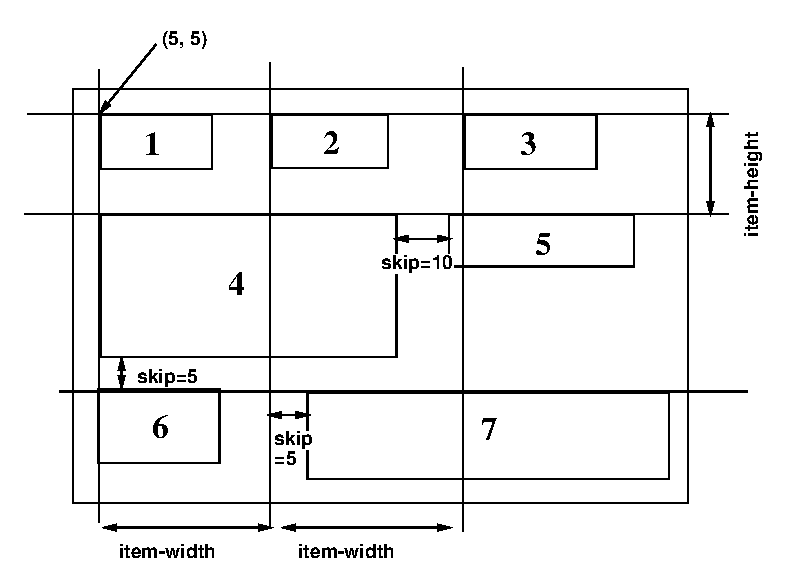
\includegraphics[height=7cm]{fig/panellayout.ps}
%\epsfile{file=fig/panellayout.ps,height=7cm}
\end{center}
\caption{panelのアイテムレイアウト\label{panellayout}}
\end{figure}

\longdescription{:create-item}{klass label receiver method \= \&rest args
\` [メソッド]\\
\> \&key ((:font fontid)\\
\> \&allow-other-keys)}{
{\em klass}で指定されるパネルアイテムのクラス
(すなわち、{\tt button-item,  menu-button-item, slider-item, joystick-item}など),
のインスタンスを作り、{\tt :locate-item}を用いてpanelにアイテムを置く。
{\em args}は、{\em klass}の{\tt :create}メソッドに送られる。
{\em label}は、パネルアイテムの中に書かれる識別文字列である。
{\em receiver}と{\em method}は、一致するイベントを呼び出すイベントハンドラを
指定する。}

\methoddesc{:delete-items}{}{パネルアイテムを全て削除する。}
\longdescription{:create-menubar}{ \= \&rest args \`[メソッド]\\
\> \&key (:font fontid)\\
\> \&allow-other-keys}{
{\em menubar-panel}を作成し、panelの最上部に置く。}
\end{refdesc}

以下に示すメソッドは、イベントがイベントハンドラのないpanelに送られたとき、
"subclass's responsibility"警告メッセージを避けるために提供されている。
ユーザーのアプリケーションでは、これらのメソッドを上書きしなければならない。

\begin{refdesc}
\methoddesc{:quit}{\&rest a}{
{\bf window-main-loop}に{\tt :quit}メッセージを送り、
イベント処理を停止する。}
\methoddesc{:KeyPress}{event}{NILを返す。}
\methoddesc{:KeyRelease}{event}{NILを返す。}
\methoddesc{:ButtonPress}{event}{NILを返す。}
\methoddesc{:ButtonRelease}{event}{NILを返す。}
\methoddesc{:MotionNotify}{event}{NILを返す。}
\methoddesc{:EnterNotify}{event}{NILを返す。}
\methoddesc{:LeaveNotify}{event}{NILを返す。}
\end{refdesc}

\subsubsection{サブパネル(メニューとメニューバー)}

\begin{refdesc}
% menu-panel
\classdesc{menu-panel}{panel}{
 (items item-dots item-height\\
                \>charwidth charheight\\
                \>height-offset\\
                \>highlight-item\\
                \>color-pixels\\
                \>active-color)
}{
{\bf menu-panel}は、{\tt panel-button}と{\tt menu-item}のみを
含むことができるパネルの一種である。
{\tt panel}と異なり、{\tt menu-panel}はふつう見えないし、
{\tt menu-panel}と関連した{\tt button-item}が押された時に
表示される。
もし、menu-panelがいつも見えるように作られたならば、
ピンを刺したメニューとなる。
マウスイベントに対するmenu-itemの応答は、アイテムの外のどこかで
押されたマウスボタンのようにふつうのmenu-buttonと
全く異なっている。
{\tt menu-panel}を使用するためには、最初に作成し、
その中にbutton-itemを置く。
それから、{\tt menu-button-item}がpanelの中あるいはmenubarの中に
{\em :menu}の引数として{\tt menu-panel}と一緒に作成される。}

\longdescription{:create}{\&rest args \= \&key\= (:items) (:border-width 0)
   (:font font-courb12)
\` [メソッド]\\
\>\> (:width 100) (:height-offset 15) (:color *bisque1*)
                      (:active *bisque2*) \\
           \>\&allow-other-keys) 
  }{
{\bf menu-panel} windowを作成する。
そのwindowの大きさは、新しいmenu-itemが追加される時に
拡張される。}

\methoddesc{:add-item}{label name \&optional (receiver self)  \&rest mesg}{
この{\bf menu-panel} windowの中にmenuアイテムを追加し、
対応する行動を張り付ける。
マウスボタンがアイテムの上で外されたとき、
{\em receiver}オブジェクトは{\em mesg}を受け取る。}

% \methoddesc{:popup}{x y \&optional (offset 20)}{
% pops up the menu at the position (x,y) specified on the root window.}
% \methoddesc{:buttonPress}{event}{
% maps the menu-panel  and makes it visible.}
%\methoddesc{:buttonRelease}{event}{
%perform a method coresdonding toa selected item and unmap the menu window.
%}

\classdesc{menubar-panel}{panel}{}{
{\tt menubar-panel}は、親panelの最上部にいつも置かれるサブパネルである。
メニューバーに置かれるパネルアイテムは、{\tt menu-button-item}で
なければならない。
menubar-panelは、panelの{\tt :create-menubar}メソッドにより
生成される。}

\end{refdesc}

\subsubsection{ファイルパネル}
FilePanelは、ファイルやディレクトリを対話的に処理する
アプリケーションwindowである。
{\tt cd}や{\tt go-up}ボタンを使用することにより、
どんなディレクトリも見に行くことができるし、
以下の{\tt ScrollTextWindow}の中にディレクトリ内に含まれるファイルを
表示する。
テキストファイルは、異なったwindow(TextViewPanel)の中に
表示することができる。
ファイルは、また印刷することができ、削除することができ、
ボタンをクリックすることにより簡単にコンパイルすることができる。
ファイルを印刷するとき、{\tt a2ps {\em file} | lpr}コマンドがforkされたプロセスとして実行される。

\begin{figure}
\begin{center}
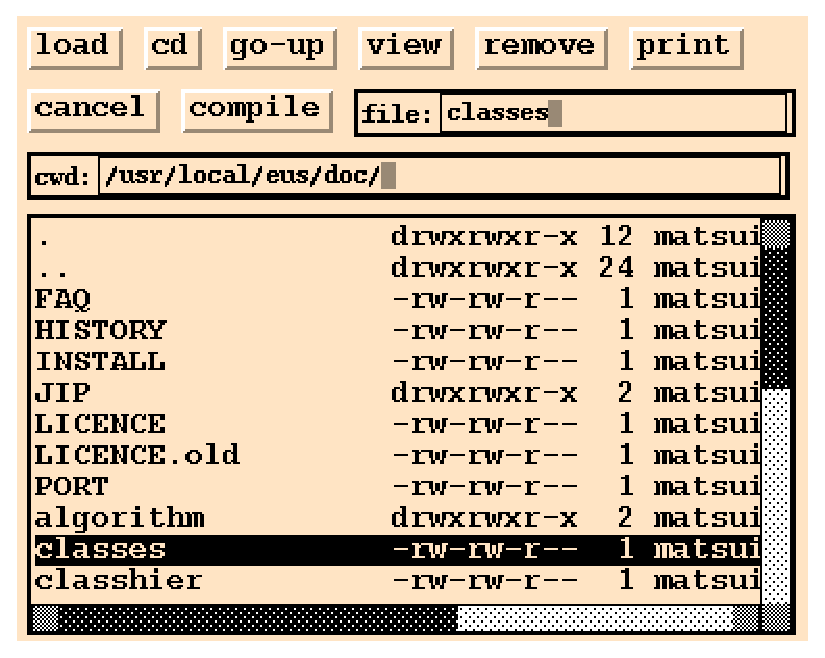
\includegraphics[height=7.5cm]{fig/filepanel.ps}
%\epsfile{file=fig/filepanel.ps,height=7.5cm}
\end{center}
\caption{ファイルパネルwindow}
\end{figure}

\subsubsection{テキスト表示パネル}

TextViewPanelは、テキストファイルを表示するための
アプリケーションwindowクラスである
(図 \ref{textviewpanel})。
プログラムテキストは、もっとも簡単なアプリケーションwindowの1つが
どのように記述されているかを見れる。
{\tt :create}メソッドにおいて、quitボタンとfindボタンと
ファイルの中を捜すための文字列を供給するためのtext-itemを
作成する。
view-windowは、縦と横にスクロールバーを持ちファイルを表示するための
ScrollTextWindowである。
TextViewPanelは、windowマネージャーにより一番外側のタイトルwindowの
大きさを変えたときview-windowの大きさを変えるために
{\tt :ConfigureNotify}イベントを捕獲する。

\begin{figure}
\begin{center}
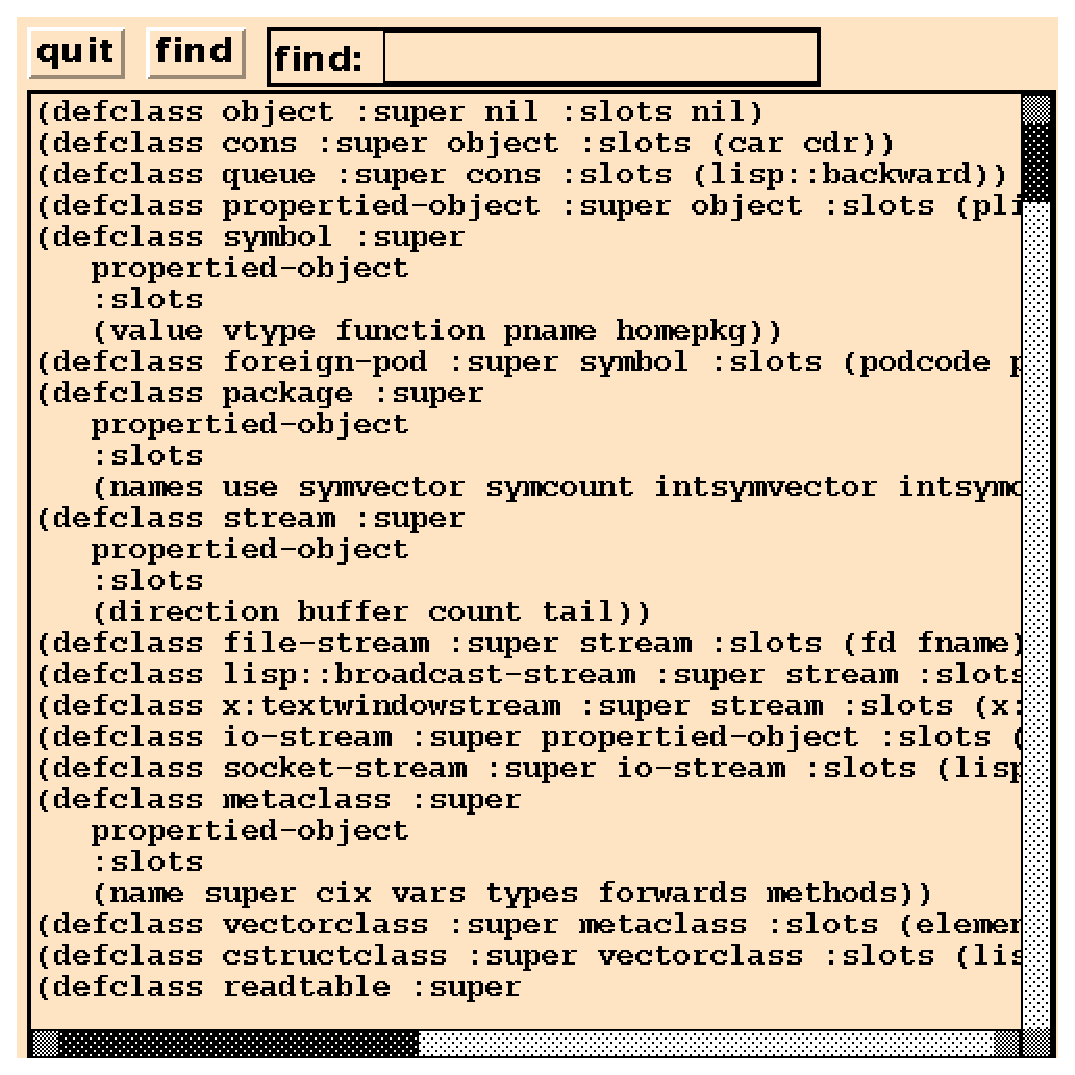
\includegraphics[height=7cm]{fig/textviewpanel.ps}
%\epsfile{file=fig/textviewpanel.ps,height=7cm}
\end{center}
\caption{テキスト表示パネルwindow\label{textviewpanel}}
\end{figure}

\begin{verbatim}
(defclass TextViewPanel :super panel
        :slots (quit-button find-button find-text view-window))

(defmethod TextViewPanel
 (:create (file &rest args &key (width 400) &allow-other-keys)
    (send-super* :create :width width args)
    (setq quit-button
          (send self :create-item panel-button "quit" self :quit))
    (setq find-button
          (send self :create-item panel-button "find" self :find))
    (setq find-text
          (send self :create-item text-item "find: " self :find))
    (setq view-window
            (send self :locate-item
                (instance ScrollTextWindow :create
                   :width (setq width (- (send self :width) 10))
                   :height (- (setq height (send self :height)) 38)
                   :scroll-bar t :horizontal-scroll-bar t
                   :map nil      :parent self)))
    (send view-window :read-file file))
 (:quit (event)  (send self :destroy))
 (:find (event)
    (let ((findstr (send find-text :value)) (found)
          (nlines (send view-window :nlines)))
        (do ((i 0 (1+ i)))
            ((or (>= i nlines) found))
           (if (substringp findstr (send view-window :line i)) (setq found i)))
        (when found
           (send view-window :display-selection found)
           (send view-window :locate found))))
 (:resize (w h)
    (setq width w height h)
    (send view-window :resize (- w 10) (- h 38)))
 (:configureNotify (event)
   (let ((newwidth (send self :width))
         (newheight (send self :height)))
        (when (or (/= newwidth width) (/= newheight height))
          (send self :resize newwidth newheight)))  ) )
\end{verbatim}

\subsection{パネルアイテム}
\begin{refdesc}
\classdesc{panel-item}{xwindow}
{(pos notify-object notify-method\\
\>fontid label labeldots)}{
{\bf panel-item}は、パネルアイテムwindowのすべての種類において、
アイテムが指定するイベントが発生したとき
{\tt notify-object}の{\tt notify-method}を呼び出すための
抽象クラスである。
}

\methoddesc{:notify}{\&rest args}{
{\tt notify-object}の{\tt notify-method}を呼び出す。
イベント応答や{\tt notify-method}へ送るための引き数が
アイテムにより区別される。
\begin{description}
\item [button-item] ボタンは、同じbutton-itemの押し、外し時に応答。
引き数はbutton-itemオブジェクトである。
\item [menu-button-item] メニューアイテムの選択時に応答。
引き数は、menu-button-itemオブジェクトである。
\item [choice-item] 新しい選択ボタンの選択時に応答。
引き数は、choice-itemオブジェクトとその選択番号である。
\item [text-item] 改行あるいはリターンの入力時に応答。
引き数は、text-itemオブジェクトと入力行(文字列)である。
\item [slider-item] スライダーノブは、つかみと移動時に応答。
引き数は、slider-itemオブジェクトと新たな値である。
\item [joystick-item] ジョイスティックは、つかみと移動時に応答。
引き数はslider-itemオブジェクトと新しいxとyの値である。
\end{description}
}

\longdescription{:create}{name reciever method \= \&rest args
\` [メソッド] \\
\> \&key ((:width w) 100) ((:height h) 100) (:font font-courb12)\\
\> \&allow-other-keys}{
パネルアイテムを作成する。
パネルアイテムは、抽象クラスである。
このメソッドは、サブクラスによって{\tt send-super}を通してのみ
呼び出すべきである。}

\classdesc{button-item}{panel-item}{}{
{\bf button-item}は、簡単なパネルアイテムである。
button-itemは、四角ボックスとその中のラベル文字列を持っている。
クリックされたとき、button-itemはpanel-itemオブジェクトを唯一の引き数として
{\tt notify-object}の{\tt notify-method}
を呼び出す。}

\methoddesc{:draw-label}{\&optional (state :top) (color bg-color) (border 2) (offset)}{
{\bf button-item}のラベルを書く。}

\longdescription{:create}{label revciever method \= \&rest args
\` [メソッド]\\
\>\&key\= :width :height (:font (send parent :gc :font))\\
\>\> (:background (send parent :gc :background)) \\
\>\> (:border-width 0) \\
\>\> (:state :top)\\
\>\&allow-other-keys}{
{\bf button-item}を作成する。
もし、ボタンの幅と高さが与えられないなら、サイズは
与えられたフォントを用いて書かれた
ラベル文字列に合わせて自動的に設定される。
{\em :border-width}はデフォルトで0であるが、
擬似3次元表現でボタンを浮き出しにする。
背景やフォントは親window(すなわち、panel)で定義されているものを
デフォルトとする。}

\methoddesc{:ButtonPress}{event}{
もし、ボタンであれば、背景色をグレーにする。}

\methoddesc{:ButtonRelease}{event}{
{\em event}の背景色を標準に変更する。}


\classdesc{menu-button-item}{button-item}{(\= items item-dots item-labels\\
\>charwidth charheight \\
\>menu-window window-pos high-light)
}{
プルダウンメニューを定義する。
{\bf menu-button-item}は、{\tt button-item}のようであるが、
{\bf menu-button-item}は、ボタンの下の関連する{\tt menu-panel}が
押されたとき、
{\tt notify-object}にすぐにメッセージを送る代わりに、
活性化させる。
メニューアイテムの1つの上でマウスボタンが外されたときに、本当のメッセージが
送られる。}

\longdescription{:create}{\= label reciever method \` [メソッド]\\
\>\&rest args\\
\>\&key (:menu nil) (:items) (:state :flat)\\
\>\&allow-other-keys}{
プルダウンメニューを作成する。
{\em receiver}と{\em method}引き数は、影響を与えない。}

\methoddesc{:ButtonPress}{event}{
プルダウンメニューのボタンを反転させ、
ボタンの下に関連するmenu-panelをさらす。}

\methoddesc{:ButtonRelease}{event}{
このボタンの下の{\tt menu-panel}を消し、
このボタンを元に戻す。}

% Bitmap-button-item
\classdesc{bitmap-button-item}{button-item}{
(pixmap-id bitmap-width bitmap-height)
}{
{\bf bitmap-button-item}の関数は、{\tt button-item}に似ているが、
表現が異なっている。
{\tt button-item}の場合にボタンの上に簡単なラベル文字列を描く代わりに、
{\tt bitmap-button-item}では、ボタンが作られたときにbitmapファイルから
ロードされるpixmapを描く。}

\longdescription{:create}{ bitmap-file reciever method \= \&rest args
\` [メソッド]\\
                 \>\&key :width :height\\
                 \>\&allow-other-keys)
}{
{\bf bitmap-button-item}を作成する。
最初の引き数{\em bitmap-file}は、{\tt button-item}の{\em label}引き数
を置き換えたものである。}

\methoddesc{:draw-label}{\&optional (state :flat) (color bg-color) (border 2)}{
ボタンの上にbitmapかpixmapを描く。}

\methoddesc{:create-bitmap-from-file}{fname}{
{\em fname}という名のbitmapファイルからpixmapを作り、
{\tt pixmap-id}にそのIDを入れる。}

% choice-item
\classdesc{choice-item}{button-item}{
 (choice-list active-choice transient-choice \\
                \>choice-dots choice-pos button-size)
}{
{\bf choice-item}は、丸い選択ボタンの集合である。
1つの選択はいつも活性化しており、同時に1つの選択だけが
活性化することができる。
{\bf choice-item}は、ラジオボタンと同様な機能を提供する。}

\longdescription{:create}{label reciever method \= \&rest args
\` [メソッド]\\
           \>\&key \=(:choices '("0" "1")) (:initial-choice 0)\\
\>\> (:font (send parent :gc :font))\\
                \>\>(:button-size 13)\\
                \>\>(:border-width 0)\\
  }{
{\bf choice-item-button}を作成する。
それぞれの選択ボタンは{\em :button-size}の半径を持つ円である。
新しい選択ボタンが選択されたとき、
{\tt notify-object}の{\tt notify-method}が
choice-itemオブジェクトと選択された選択ボタンの番号と一緒に呼び出される。}

\methoddesc{:value}{\&optional (new-choice) (invocation)}{
もし、{\em new-choice}が与えられたならば、現在の活性化選択ボタンとして
設定し、対応する円が黒色になる。
もし{\em  invocation}も指定されているなら、{\tt notify-object}の
{\tt notify-method}が呼び出される。
{\tt :value}は、現在の(あるいは新しい)選択ボタンの番号を返す。}

\methoddesc{:draw-active-button}{\&optional
(old-choice active-choice) (new-choice active-choice)}{
ボタンを活性化として書く。
}

\methoddesc{:ButtonPress}{event}{
もし、選択ボタンのどこかでマウスボタンが押されているなら、
その番号が{\tt transient-choice}に記録される。
マウスボタンが外されるまでそれ以上の行動は、起こさない。}

\methoddesc{:ButtonRelease}{event}{
もし、既に押されていたところと同じボタンの上でマウスボタンが外されたなら、
{\tt active-choice}が更新され、
{\tt notify-object}の{\tt notify-method}が呼び出される。
}

% Slider-item
\classdesc{slider-item}{panel-item}{
(min-value max-value value\\
                \>minlabel maxlabel valueformat\\
                \>bar-x bar-y bar-width bar-height valuedots label-base\\
                \>nob-x nob-moving\\
                \>charwidth) 
}{
{\tt choice-item}が離散的な値の選択に使用されるのに対し、
{\bf slider-item}は{\tt min-value}と{\tt max-value}の間の範囲の
連続的な値に対して使用される。
それぞれ値が変化した瞬間、slider-itemオブジェクトと新しい値が引き数として
一緒に{\tt notify-object}の{\tt notify-method}が呼び出される。}

\longdescription{:create}{label reciever method \= \&rest args
\` [メソッド]\\
\>\&key (:min 0.0) (:max 1.0) (:parent)\\
\>(:min-label "") (:max-label "") (:value-format "~4,2f")\\
\>(:font font-courb12) (:span 100) (:border-width 0) (:initial-value min)  }{
{\bf slider-item}を作成する。
スライドのノブは、バーの上に小さな黒の四角として表示される。
左端が{\em :min}値を表現し、右端が{\em :max}値を表現する。
バーの長さは、{\em :span}ドットに引き伸ばす。
現在の値は、{\em :value-format}でslider-itemの右に表示する。}

\methoddesc{:value}{\&optional newval invocation}{
もし、{\em newval}が与えられたなら、現在の値として設定され、
ノブは対応する位置にスライドする。
もし、{\em invocation}もnon NILに指定されていたなら、
{\tt notify-object}の{\tt notify-method}が呼び出される。
{\tt :value}は、現在の(新しい)値を返す。}

% JoyStick-item
\classdesc{joystick-item}{panel-item}{
 (stick-size min-x min-y max-x max-y\\
                \>center-x center-y stick-x stick-y\\
                \>value-x value-y\\
                \>stick-return stick-grabbed\\
                \>fraction-x fraction-y)
}{
{\bf joystick-item}は、2次元のslider-itemとしてみなすことができる。
2つの連続値はクモの巣のような同心円図の上を動く黒い円によって
指定することができる(図 \ref{panelitem})。}

\longdescription{:create}{name reciever method \= \&rest args
\` [メソッド]\\
           \>\&key \=(:stick-size 5) (:return nil)\\
                \>\>(:min-x -1.0) (:max-x 1.0)\\
                \>\>(:min-y -1.0) (:max-y 1.0)\\
           \>\&allow-other-keys) 
  }{
{\em :stick-size}は、スティックの黒い円の半径である。
同心円図の円の大きさは、{\bf joystick-item} windowの幅と高さ
に合うように決定される。
もし、{\em :return}がnon NILであるなら、
ジョイスティックは、マウスボタンが外された時の原点に帰る。
そうでないなら、ジョイスティックは、外された位置に残る。}


%\methoddesc{:draw-circles}{}{
%}
%\methoddesc{:xy}{\&optional (x value-x) (y value-y)}{
%}
%\methoddesc{:draw-stick}{\&optional (x value-x) (y value-y) (erase t)}{
%}
\methoddesc{:value}{\&optional (newx) (newy) (invocation)}{
もし、{\em newx}と{\em newy}が与えられたなら、
現在の位置として設定され、ジョイスティックは同心円図の
対応する位置に移動する。
もし、{\em invocation}もnon NILに指定されたなら、
{\tt notify-object}の{\tt notify-method}が、
{\bf joystick-item}オブジェクトとx,y値を引き数として一緒に呼び出される。
{\tt :value}は、現在の(新しい)値のリストを返す。}

\end{refdesc}

以下に上に記述されているpanel-itemを使った短いプログラムを示し、
図 \ref{panelitem}がパネルの中にどのように表示されるかを示したものである。

\begin{verbatim}
(in-package "X")
(defclass testPanel :super panel
        :slots (quit joy choi sli))
(defmethod testPanel
 (:create (&rest args)
    (send-super* :create :width 210 :height 180 
                 :font font-courb12 args)
    (send-super :create-item button-item "quit" self :quit :font font-courb14)
    (send-super :create-item choice-item "choice" self :choice
                :choices '(" A " " B " " C ")
                :font font-courb12)
    (send-super :create-item slider-item "slider" self :slider
                :span 90)
    (send-super :create-item joystick-item "joy" self :joy)
    self)
 (:choice (obj c) (format t "choice: ~S ~d~%" obj c))
 (:slider (obj val) (format t "slider: ~S ~s~%" obj val))
 (:joy (obj x y) (format t "joy: ~S ~s ~s~%" obj x y)) )
(instance testPanel :create)
(window-main-thread)
\end{verbatim}

\begin{figure}
\begin{center}
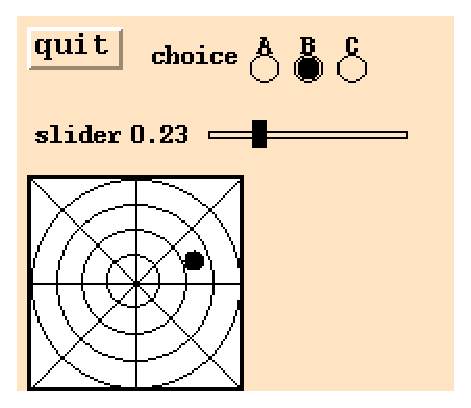
\includegraphics[height=5cm]{fig/panelitem.ps}
%\epsfile{file=fig/panelitem.ps,height=5cm}
\end{center}
\caption{panelの中に作成されたpanel-item\label{panelitem}}
\end{figure}

\begin{refdesc}
\classdesc{text-item}{panel-item}
{(textwin)}{
{\bf text-item}は、ファイル名のような短いテキストを表示したり入力したり
するために使用する。
{\bf text-item}は、ラベル文字列とその右側に小さなテキストwindowを持っている。
テキストwindow内にポインタが置かれたとき、キー入力が可能となり、
入力された文字がバッファに入れられる。
テキストwindow内の行修正が可能である。
{\tt control-F}と{\tt control-B}は前後に1文字動かし、
{\tt del}はカーソルの左の1文字を削除し、
{\tt control-D}はカーソル位置の文字を削除し、
カーソル位置にはどんなグラフィック文字も挿入できる。
マウスボタンをクリックすれば、クリックされた文字にカーソルを
移動させる。
enter(改行)キーを打つことにより、バッファされたテキストが
{\tt notify-object}の{\tt notify-method}に送られる。}

\longdescription{:create}{label revciever method \= \&rest args \` [メソッド]\\
\>\&key (:font font-courb12) (:columns 20) (:initial-value ) (:border-width 0)\\
\>\&allow-other-keys}{
{\bf text-item}を作成する。
テキストwindowの行バッファには、長さの制限が無いけれども、
見える部分は{\em columns}文字に制限されている。}

\methoddesc{:getstring}{}{
キーバッファ内の文字列を返す。}

%\methoddesc{:KeyPress}{pos}{
%if key is pressed, print key character to cursor position.}

%\methoddesc{:keyEnter}{ch}{
%prints {\em ch} to cursor position. But if {\em ch} is backspace,
%deletes 1 character from buffer. And if {\em ch} is return or newline,
%ignores.}
\end{refdesc}

\subsection{キャンバス}
\begin{refdesc}
\classdesc{canvas}{xwindow}{(topleft bottomright)}{
{\bf canvas}は、図や画像を入れるためのXwindowである。
現在、領域選択機能のみ実現されている。
ButtonPressイベントにより、{\bf canvas}は押された位置を左上の端とし、
現在の位置を右下の端とする四角を描き始める。
ButtonReleaseにより、{\tt notify-object}の{\tt notify-method}が
送られる。
canvas内に図や画像を描くためにはXdrawableのメソッドが使用される。}

%\methoddesc{:adjust-corners}{}{
%corrects toleft and bottomright.}

%\methoddesc{:region-selection}{}{
%prints canvas region.}

%\methoddesc{:draw-selection-rectangle}{}{
%draws a rectangle that shows canvas region.}

%\methoddesc{:ButtonPress}{event}{
%reverses the color of button that shows {\em event}.}
%\methoddesc{:MotionNotify}{event}{
%makes selection rectangle which corners are pressed position 
%and cursor position.}
%\methoddesc{:ButtonRelease}{event}{
%clears selection rectangle and prints item on this canvas region.}

%\methoddesc{:clear-canvas}{item}{
%ignores {\em item}.}

\end{refdesc}

\subsection{テキストwindow}

{\tt TextWindow}と{\tt BufferTextWidnow}と{\tt ScrollTextWindow}の
3つのテキストwindowがある。

\begin{refdesc}
\classdesc{textWindow}{xwindow}
{(fontid \\
\>charwidth charheight charascent dots \\
\>win-row-max win-col-max \\
\>win-row win-col \hspace{20mm} \= ;physical current position in window \\
\>x y\\
\>charbuf \>; for charcode conversion \\
\>keybuf keycount \> ;for key input\\
\>echo \\
\>show-cursor cursor-on \> ;boolean\\
\>kill delete \> ;control character \\
\>notify-object notify-method \\
\>)}{
メッセージを表示するために使用可能な仮想端末を実現する。
表示される内容は、バッファされないし、{\bf TextWindow}に既に表示された
文字や行を引き出す方法はない。
基本的に、{\bf TextWindow}は
カーソル移動、行削除、領域削除、表示テキストのスクロール、文字列挿入
などを持つダンプ端末と似た能力を持っている。
また、テキストカーソルはマウスポインタで指示された位置に
移動することができる。}

\methoddesc{:init}{id}{
{\em id}番目のテキストwindowを初期化する。}

\longdescription{:create}{\=\&rest args \` [メソッド]\\
\>\&key \=:width :height (:font font-courb14) :rows :columns\\
\>(:show-cursor nil) (:notify-object nil) (:notify-method nil)\\
\>\&allow-other-keys}{
text-windowを作成する。
windowの大きさは、{\em :width}と{\em :height}かあるいは{\em :rows}と
{\em :columns}で指定されたものとなる。
{\em :notify-object}の{\em :notify-method}は、改行文字が入力された
ときに呼び出される。}

%\methoddesc{:set-notify}{reciever method}{
%}

\methoddesc{:cursor}{flag}{
{\em flag}は、{\tt :on, :off, :toggle}のどれかが可能である。
テキストカーソルは、{\tt win-row}と{\tt win-col}の位置である。
もし、{\em flag}が{\tt :on}であれば、テキストカーソルは表示され、
{\em flag}が{\tt :off}ならば、消される。
また、{\em flag}が{\tt toggle}ならば、反対になる。
このメソッドは、カーソルの位置の文字を更新するときはいつでも、
呼び出されなければならない。}

\methoddesc{:clear}{}{
テキストwindow内を消去する。}

\methoddesc{:clear-eol}{\&optional (r win-row) (c win-col) (csr :on)}{
{\em r}と{\em c}で指定される位置の文字以降の残りの行を
消去する。カーソル位置の文字も含む。}

\methoddesc{:clear-lines}{lines \&optional (r win-row)}{
{\em r}番目の行以降の複数行を消去する。}

\methoddesc{:clear-eos}{\&optional (r win-row) (c win-col)}{
{\em r}と{\em c}で指定される位置から画面の最後までの領域を消去する。}

\methoddesc{:win-row-max}{}{このwindowに表示可能な最大行数を返す。}

\methoddesc{:win-col-max}{}{このwindowに表示可能な最大列数を返す。}

\methoddesc{:xy}{\&optional (r win-row) (c win-col)}{
{\em r}と{\em c}で指定される位置の文字のピクセル座標を計算する。}

\methoddesc{:goto}{r c \&optional (cursor :on)}{
{\em r}番目の行の{\em c}番目の列にカーソルを移動する。}

\methoddesc{:goback}{\&optional (csr :on)}{
カーソルを1文字戻す。}

\methoddesc{:advance}{\&optional (n 1)}{
{\em n}文字だけカーソルを進める。}

\methoddesc{:scroll}{\&optional (n 1)}{
{\em n}行だけ縦方向にテキストwindowをスクロールする。}

\methoddesc{:horizontal-scroll}{\&optional (n 1)}{
{\em n}列だけ横方向にテキストをスクロールする。}

\methoddesc{:newline}{}{
次の行の最初にカーソルを移動する。}

\methoddesc{:putch}{ch}{
カーソル位置に文字{\em ch}を挿入する。
行の残りは、1文字前方に進められる。}

%\methoddesc{:putstr}{str \&optional (e (length str))}{
%prints {\em str} to text-window.}
%
\methoddesc{:putstring}{str \&optional (e (length str))}{
カーソル位置に{\em str}を置く。}

%\methoddesc{:getstring}{}{gets key-buffer.}

\methoddesc{:event-row}{event}{}
\methoddesc{:event-col}{event}{
{\em event}における、テキストカーソルの位置をを返す。}
%\methoddesc{:EnterNotify}{event}{}
%\methoddesc{:ButtonPress}{event}{}
%\methoddesc{:ButtonRelease}{event}{}
%\methoddesc{:resize}{w h}{}
%\methoddesc{:ConfigureNotify}{event}{}
%\methoddesc{:keyrelease}{}{nob}
%\methoddesc{:enterNotify}{event}{}
%\methoddesc{:LeaveNotify}{event}{}
\methoddesc{:KeyPress}{event}{
カーソル位置に入力された文字を挿入する。
もし、文字が改行であったなら、{\tt notify-object}に通知する。}
%\methoddesc{:keyEnter}{ch}{}
%\methoddesc{:LineEnter}{ch}{}
%\methoddesc{:clear-text}{item}{clear text-window.}

\classdesc{TextWindowStream}{stream}{(textwin)}{
{\tt TextWindowStream}は、TextWdinowに接続された出力ストリームである。
{\tt print, format, write-byte}などによってこのストリームに出力
される文字や文字列がTextWdindowに表示される。
通常のファイルストリームとしては、
出力データはバッファされる。}

\methoddesc{:flush}{}{
バッファされたテキスト文字列を掃き出し、TextWindowに送る。
{\tt finish-output}やこのストリームへの改行文字の書き込みは、
このメソッドを自動的に呼び出す。}

\funcdesc{make-text-window-stream}{xwin}{
{\bf text-window-stream}を作り、そのストリームオブジェクトを返す。}

\classdesc{BufferTextWindow}{TextWindow}{
(linebuf expbuf max-line-length row col)}{
{\bf TextWindow}の内容を表現する行バッファを保持する。
{\tt linebuf}は、行のベクトルである。{\tt exbuf}は、
タブ拡張されたテキストを持つ。
windowに表示可能な行のみが保持される。
{\bf BufferTextWindow}は、数行のテキストを持つ
簡単なテキストエディタとして使用することができる。
{\tt text-item}は、表示可能な行バッファとして{\bf BufferTextWindow}を
使う。}

%\methoddesc{:create}{\&rest args}{}
%\methoddesc{:clear}{}{}
%\methoddesc{:goto}{r c \&optional (csr :on)}{}
\methoddesc{:line}{n}{
{\em n}番目の行の内容を文字列として返す。}

\methoddesc{:nlines}{}{{\tt linebuf}の行数を返す。}
\methoddesc{:all-lines}{}{文字列のベクトルである{\tt linebuf}を返す。}
\methoddesc{:refresh-line}{\&optional (r win-row) (c win-col)}{
{\em r}番目の行の{\em c}番目の列以降を再書き込みする。}
\methoddesc{:refresh}{\&optional (start 0)}{
{\em start}番目の行以降の行を再書き込みする。}
\methoddesc{:insert-string}{string}{
カーソル位置に{\em string}を挿入する。}
\methoddesc{:insert}{ch}{カーソル位置に文字を挿入する。}
\methoddesc{:delete}{n}{カーソル以降の{\em n}文字を削除する。}
%\methoddesc{:KeyEnter}{ch \&optional event}{}
%\methoddesc{:ButtonRelease}{event}{}

\funcdesc{expand-tab}{src \&optional (offset 0)}{
{\em src}は、タブを含んだ可能性のある文字列である。
これらのタブは、タブの停止位置が8の倍数であると仮定して空白文字に
置き換えられる。}

\classdesc{ScrollTextWindow}{BufferTextWindow}{
(top-row top-col \hspace{30mm} \= ;display-starting position \\
\> scroll-bar-window \\
\> horizontal-scroll-bar-window \\
\> selected-line)}{
{\bf ScrollTextWindow}は、行数制限がなく、縦と横にスクロールバーを持った
{\tt BufferTextWindow}を定義する。
{\bf ScrollTextWindow}は、スクロールバーを伴ってwindowの大きさを変更するため、
あるいはテキストを再表示するために{\tt :configureNotify}イベントを
扱うことができる。
クリックすることによって、行を選択することができる。}

\methoddesc{:create}{\&rest args
           \&key (scroll-bar nil)
                (horizontal-scroll-bar nil)
           \&allow-other-keys}{
スクロールバーが必要なとき、それぞれのキーワードの引き数にTを指定する。}

%\methoddesc{:locate-scroll-bar}{}{}
%\methoddesc{:clear}{}{}
%\methoddesc{:lines}{}{}
%\methoddesc{:max-line-length}{}{}
%\methoddesc{:refresh}{\&optional (offset 0) (lines (- win-row-max offset))}{}
%\methoddesc{:line-in-window-p}{ln}{}
%\methoddesc{:refresh-line}{ln \&optional (highlight nil) \&aux fg-save bg-save}{
%}
\methoddesc{:locate}{n}{windowの上部から{\em n}番目の行に
バッファされたテキストを表示する。}
\methoddesc{:display-selection}{selection}{
{\em selection}は、選択された行の位置を表現する。
選択された行がすべて高輝度で表示される。}

\methoddesc{:selection}{}{選択された行(文字列)を返す。}

\methoddesc{:read-file}{fname}{
{\em fname}で指定されるテキストファイルを{\tt linebuf}に読み込み、
タブを拡張し、windowに表示する。
カーソルは、画面の最初に置かれる。}

\methoddesc{:display-string}{strings}{
{\em strings}は、行(文字列)の列である。
{\em strings}は、{\tt linebuf}にコピーされ、windowに表示される。}

%\methoddesc{:scroll-fraction}{}{}
%\methoddesc{:horizontal-scroll-fraction}{}{}

\methoddesc{:scroll}{n}{{\em n}行、縦にスクロールする。}
\methoddesc{:horizontal-scroll}{n}{{\em n}列、横にスクロールする。}
%\methoddesc{:insert-char}{c \&optional (refresh t)}{}
%\methoddesc{:insert-newline}{\&optional (refresh t)}{}
%\methoddesc{:insert}{thing \&optional (refresh t)}{}
%\methoddesc{:buttonPress}{event}{}
\methoddesc{:ButtonRelease}{event}{
マウスポインタが置かれている行が選択される。
もし、windowが作成されたときに{\tt notification}が指定されている
ならば、{\tt notify-object}の{\tt notify-method}が呼び出される。}

\methoddesc{:resize}{w h}{
windowの大きさを変更し、新しいサイズに合うように
内容を再表示する。
もし、スクロールバーがあれば、同じメッセージが送られる。}
%\methoddesc{:ConfigureNotify}{event}{}

%\classdesc{xitem}{xwindow}
%{(label labeldots width height)}{
%defines xitem that is used for pulldown menu.}

%\methoddesc{:draw-label}{}{
%draws xitem's label.}

%\longdescription{:create}{label \= \&rest args \hspace{120mm} [method]\\
%\>\&key width height (font font-cour10)\\
%\>\&allow-other-keys}{
%creates xitem.}

% \classdesc{input-panel}{panel}{}{
% defines input-lines for panel. Input-panel is a one line input window that
% has quit button, cancel button and input line with under-line. 
% This class is used by xinput function.}
% 
% \methoddesc{:getstring}{}{
% gets key-buffer.}
% 
% \methoddesc{:quit}{\&rest args}{
% quit this input line window.}
% 
% \methoddesc{:input-line}{\&rest args}{
% quit this input line window.}
% 
% \methoddesc{:create}{title len \&rest args}{
% creates input line window. And add 'CANCEL' button on this window.}
% 
%\funcdesc{xitem-length}{label \&key (font font-cour10)}{
%returns {\em label}'s length.}

%\funcdesc{xset-eachground}{win fg bg \&optional (f-flag t)}{
%sets {\em win}'s foreground color and background color. And {\em win} refresh.
%But if {\em f-flag} is nil, {\em win} don't refresh.}

% \funcdesc{x::xinput}{\&key (title "Input:") (len 30) (font font-cour10) (par *root*) x y}{
% creates input-panel positioned ({\em x},{\em y}), then gets string. 
% If input is end, returns input string, and destroys this input-panel. 
% When input string is nothing, returns nil. Notes that mouse cursor have
% to be moved on the input area, whenever you input text.}

\end{refdesc}

\newpage

\section{画像処理}

\markright{\arabic{section}. 画像処理}
画像処理の諸機能は,{\tt "vision/piximage"}ファイルに格納されている。
画像データを表現するために2つのクラス
{\bf pixel-image}と{\bf color-pixel-image}が定義されている。
ルックアップテーブル(LUT)を用いたピクセル(pixel)毎の変換,
エッジ抽出,pbmファイルへの画像データの変換が実現されている。

\subsection{ルックアップテーブル (LUT)}
LUTは,ピクセル(pixel)データを変換するためのベクトルデータである。 

\begin{refdesc}

\funcdesc{make-equilevel-lut}{levels \&optional (size 256)}{
1次元の整数ベクトル(integer-vector)を返す。
そのベクトルは,0から{\em size}までの値を0から{\em levels}までの値に
線形的にマップする。
例えば,{\tt (make-equilevel-lut 3 12)}は,
{\tt \#i(0 0 0 0 1 1 1 1 2 2 2 2)}を返す。}

\funcdesc{look-up}{src dest lut}{
ルックアップテーブル{\em lut}を用いて{\em src}ベクトルを{\em dest}ベクトルに
値を変換して置き換える。 もし{\em dest}ベクトルがNILのときは,
{\em src}ベクトルと同じクラスで同じサイズのベクトルを作る。
例えば, {\tt (look-up \#i(1 2 3) nil \#(10 20 30 40 50))}は,
{\tt \#i(20 30 40)}を返す。}

\funcdesc{look-up2}{src dest lut1 lut2}{
{\bf look-up2}は、ルックアップテーブル{\em lut1}および{\em lut2}を連続的に使用して
{\em src}ベクトルを{\em dest}ベクトルに変換する。
{\em src}と{\rm dest}は、同じサイズの整数ベクトルあるいはバイトベクトル(文字列)である。}


\funcdesc{look-up*}{src dest luts}{
{\em luts}は,ルックアップテーブルのリストである。
{\em luts}から与えられるルックアップテーブルを連続的に使用して,
{\em src}ベクトルを{\em dest}ベクトルに変換する。}

\funcdesc{concatenate-lut}{lut1 lut2 \&optional (size 256)}{
2つのルックアップテーブル{\em lut1}と{\em lut2}をつないだ
新しいルックアップテーブルを返す。その新しいテーブルを使用することは,
{\em lut1}と{\em lut2}を連続的に使用することと同じである。}

\funcdesc{make-colors}{default-color-map}{
以下に示すデフォルトのカラーマップを作る。}

\vardesc{*x-gray32-lut*}{
デフォルトカラーマップ{\tt x:*colormap*}
に定義されている32階調のグレースケールのLUTである。
{\tt (aref *x-gray32-lut* n)}は,32階調の内のn番目のグレー階調を返す。}

\vardesc{*x-gray16-lut*}{
デフォルトカラーマップ{\tt x:*colormap*}
に定義されている16階調のグレースケールのLUTである。}

\vardesc{*x-color-lut*}{
デフォルトカラーマップ{\tt x:*colormap*}
に定義されている幾つかの鮮明なカラーのLUTである。
登録されているカラーは, "black", "red", "green", "lightblue", "yellow",
"orange", "blue", "magenta", "white"である。}

\vardesc{*256to8*}{
0..255の範囲の整数を0..7の範囲に変換する256入力のLUTである。
その階調は,線形にマップされている。}

\vardesc{*256to16*}{
0..255の範囲の整数を0..15の範囲に変換する256入力のLUTである。
その階調は,線形にマップされている。}

\vardesc{*256to32*}{
0..255の範囲の整数を0..31の範囲に変換する256入力のLUTである。
その階調は,線形にマップされている。}

\vardesc{*gray32*}{
グレースケールピクセルをXのカラーマップに変換するための256入力のLUTである。
これは、{\tt *256to32*}と{\tt *x-gray32-lut*}を連結して作られる。
グレー32階調のXwindowの表示可能なピクセル画像は{\bf *gray32*}によって
グレー256階調の画像を変換することにより得ることができる。}

\vardesc{*rainbow32*}{
256階調のhue値をXのレインボーカラーマップに変換する
ための256入力のLUTである。
これは、{\tt *256to32*}と{\tt *x-rainbow32-lut*}を連結して作られる。}

\end{refdesc}

\subsection{ピクセル画像}
1枚の画像データは、{\bf pixel-image}クラスで表現される。{\bf pixel-image}は、
バイト型データを要素とする2次元配列である。それぞれのデータの内容は、
アプリケーションに依存している。一般的にピクセルの明るさを表現するために
使われるが、エッジ輝度や微分方向やカラー輝度やbarグラフのようなものにも用いることができる。

\begin{refdesc}
\classdesc{pixel-image}{array}{xpicture display-lut histogram\\
\>brightness-distribution0\\
\>brightness-distribution1\\
\>brightness-covariance}{
%provides a way to define image data with their horizontal/vertical sizes.
{\bf pixel-image}は、xwindowへの表示機能を持つ2次元の行列である。
pixelの変換は、{\bf display-lut}によって実現され、
その結果の画像は{\em xpicture}に蓄積される。
主な軸は縦方向にとる。{\tt (x,y)}の{\tt img}のピクセルは
{\tt (aref img y x)}でアクセスすることができる。}

\methoddesc{:width}{}{ピクセル画像の横サイズを返す。}
\methoddesc{:height}{}{ピクセル画像の縦サイズを返す。}
\methoddesc{:size}{}{配列の大きさを返す。}
\methoddesc{:transpose}{
\&optional (result (instance (class self) :init dim0 dim1))}{
x軸とy軸を交換する。}
\methoddesc{:map-picture}{lut \&optional (result (send self :duplicate))}{
この画像を{\em lut}で変換し、その画像データを{\em result}に蓄積する。}
\methoddesc{:map}{fn \&optional (result (send self :duplicate))}{
この画像のすべてのピクセルに{\em fn}を適用して、
{\em result}のピクセルに置く。}
\methoddesc{:brightest-pixel}{}{この画像の一番明るいピクセル値を見つける。}
\methoddesc{:darkest-pixel}{}{この画像の一番暗いピクセル値を見つける。}
\methoddesc{:average-pixel}{}{
この画像のすべてのピクセルの平均輝度を計算する。}
\methoddesc{:halve}{\&optional simage}{
半分の大きさの画像に縮小したピクセル画像を返す。}
% (:expand (rate) )
\methoddesc{:subimage}{x y subwidth subheight}{
この画像に{\em (x,y)}を左上角とし、幅が{\em subwidth}で高さが{\em subheight}
である四角形を切り出す。
その画像の原点は{\em (x,y)}に置かれる。
{\tt :subimage}は、この四角形で囲まれた画像を表現するピクセル画像を作る。}
\methoddesc{:xpicture}{\&optional lut}{
この画像を{\em lut}を用いて変換し、{\tt xpicture}に設定する。}
\methoddesc{:display-lut}{\&optional newlut}{
{\tt display-lut}にルックアップテーブル{\em newlut}を設定する。
その後、このルックアップテーブルを用いて画像を変換し、
{\tt xpicture}に設定する。}
\methoddesc{:display}{(xwin geometry:*viewsurface*)}{
{\bf :putimage}を用いて{\em xwin}で指定されるXwindowにこの画像を
表示する。
それぞれのピクセル値はXのカラーマップを参照する。
希望する表現を得るためには、このピクセル画像を固有のLUTで
変換すべきである。}
\methoddesc{:duplicate}{}{
この画像オブジェクトと同じ幅と高さを持つ同じクラスの
インスタンスを作る。ピクセルデータはコピーされない。}
\methoddesc{:copy-from}{src}{
{\em src}で指定される他の画像からピクセルデータをコピーする。
{\em src}とこの画像は同一の次元でなければならない。}
\methoddesc{:hex}{\&optional (x 0) (y 0) (w 16) (h 16) (strm t)}{
四角領域で示されるピクセルデータを16進数フォーマットで表示する。}
\methoddesc{:hex1}{\&optional (x 0) (y 0) (w 64) (h 16) (strm t)}{
四角領域で示されるピクセルデータを16進数フォーマットで表示する。}
\methoddesc{:prin1}{strm \&rest msg}{
このピクセル画像を名前と次元とともに表示する。}
\methoddesc{:init}{w h \&optional imgvec}{
幅{\em w}、高さ{\em h}を持つピクセル画像を初期化する。
%もし、すべてのピクセル値が文字列ベクトルで表現されている{\em imgvec}
%が与えられたとき、その長さは{\em w*h}でなければならない。
}
\methoddesc{:amplify}{rate \&optional (result (send self :duplicate)}{
{\em rate}をそれぞれのピクセル値に掛ける。}
\methoddesc{:compress-gray-scale}{levels \&optional result  \&aux pict2}{
この画像のピクセル値を0から{\em levels}までの範囲に変換をし、
その変換された画像を返す。}
\methoddesc{:lut}{lut1 \&optional (result (send self :duplicate))}{
ルックアップテーブル{\em lut1}を用いてこの画像を変換し、
その変換された画像を返す。}
\methoddesc{:lut2}{lut1 lut2 \&optional (result (send self :duplicate))}{
{\em lut1}と{\em lut2}を連結したルックアップテーブルを用いてこの画像を
変換し、その変換された画像を返す。}
\methoddesc{:histogram}{}{
この画像のそれぞれのピクセル値の発生回数を数え、そのヒストグラム
を整数ベクトル表現で返す。}
\methoddesc{:brightness-distribution}{}{
明るさの分散を返す。}
\methoddesc{:optimum-threshold}{}{
この画像の明るさの分散値が最大となっている階調を返す。}
\methoddesc{:project-x}{}{
同じx座標のピクセル値をすべて加算し、これらの値のベクトルを返す。}
\methoddesc{:project-y}{}{
同じy座標のピクセル値をすべて加算し、これらの値のベクトルを返す。}
\methoddesc{:digitize}{threshold \&optional (val0 0) (val1 255) result}{
{\em threshold}を用いてこの画像を{\em val0}と{\em val1}の2値画像に
変換する。}
\methoddesc{:and}{img2}{
この画像と{\em img2}のビット論理積をとり、処理した画像を返す。}
\methoddesc{:plot}{min max \&optional color viewsurface}{
{\em min}と{\em max}の間の値を持つピクセルをすべて{\em color}(gc)
で{\em viewsurface}にプロットする。}

%\longdescription{:edge1}{\&optional \= (method 1) \hspace{97mm} [メソッド]\\
\longdescription{:edge1}{\&optional \= (method 1) \` [メソッド]\\
\> (th1 *edge-intensity-threshold*) (th2 *weak-edge-threshold*)\\
\> (run *edge-length-threshold*)\\
\> (win geometry:*viewsurface*) (edgeimg1)}{
この画像のエッジを抽出し、Xwindow上にエッジ画像を表示する。}
\end{refdesc}

\subsection{カラーピクセル画像}
カラー画像は、{\bf color-pixel-image}クラスで表現される。
このクラスは、3つの{\bf pixel-image}を持っており、RGB表現の
red,green,blueあるいはHLSモデルの色合い,明るさ,濃さをそれぞれ表現する。
RGBとHLS間の変換もサポートしている。
\begin{refdesc}

\classdesc{color-pixel-image}{propertied-object}
{width height component1 component2 component3}{
3つの{\tt pixel-image}オブジェクトでカラー画像を表現する。}

\methoddesc{:width}{}{この画像の幅を返す。}
\methoddesc{:height}{}{この画像の高さを返す。}
\methoddesc{:size}{}{この画像の幅$\times$高さを返す。}
\methoddesc{:red}{}{{\tt component1}を返す。}
\methoddesc{:green}{}{{\tt component2}を返す。}
\methoddesc{:blue}{}{{\tt component3}を返す。}
\methoddesc{:hue}{}{{\tt component1}を返す。
色合い(hue)の値(0〜360)は、0〜255の1バイトで表現される。}
\methoddesc{:lightness}{}{{\tt component2}を返す。
正規化された明るさ(brightness)の値(0〜1)は、0〜255の整数で表現される。}
\methoddesc{:saturation}{}{{\tt component3}返す。
正規化された濃さ(saturation)の値(0〜1)は、0〜255の整数で表現される。}
\methoddesc{:pixel}{x y}{{\em (x,y)}における
{\tt component1,component2,component3}の値を3つの整数のリストとして返す。
このリストは、RGB値あるいはHLS値のどちらでも解釈できる。}
\methoddesc{:monochromize}{\&optional (NTSC nil)}{
RGB構成から明るさを計算し、新しい{\tt pixel-image}を返す。
もし、{\em NTSC}がNILなら、{\tt (R+G+B)/3}が計算される。
もし、Tなら、{\tt 0.299*R+0.587*G+0.114*B}が計算される。}
\methoddesc{:HLS}{}{この画像をRGB画像と仮定し、HLS表現に画像を変換する。
それぞれのピクセルを変換するために{\bf RGB2HLS}を呼び出す。}
\methoddesc{:RGB}{}{この画像をHLS画像と仮定し、RGB表現に画像を変換する。
それぞれのピクセルを変換するために{\bf HLS2RGB}を呼び出す。}
\methoddesc{:halve}{}{
この画像を半分のサイズに縮小した{\bf color-pixel-image}を返す。}
\methoddesc{:display}{\&optional (win *color-viewer*)}{
{\bf :putimage}を用いて{\em win}で指定されるXwindowに
このカラー画像を表示する。
それぞれのピクセル値はXのカラーマップを参照する。
希望する表現を得るためには、この画像を固有のLUTで
変換すべきである。}
\methoddesc{:display-lut}{\&optional (newlut1) (newlut2 newlut1) (newlut3 newlut2)}{
ルックアップテーブル{\em newlut1},{\em newlut2},{\em newlut3}を
{\tt display-lut}にそれぞれ設定する。それから、このルックアップテーブルを
使ってこの画像を変換し、{\tt xpicture}に設定する。}
%\longdescription{:edge1}{\&optional \= (method 1) \hspace{97mm} [メソッド]\\
\longdescription{:edge1}{\&optional \= (method 1) \` [メソッド]\\
\> (th1 *edge-intensity-threshold*) (th2 *weak-edge-threshold*)\\
\> (run *edge-length-threshold*)\\
\> (win *color-viewer*)}{
この画像のエッジを抽出する。Xwindow上にこのエッジ画像を表示する。}
\methoddesc{:hex}{\&optional (x 0) (y 0) (w 16) (h 16) (strm t)}{
四角領域で指定されるピクセルデータを16進数フォーマットで表示する。}
\methoddesc{:hex1}{\&optional (x 0) (y 0) (w 64) (h 16) (strm t)}{
四角領域で指定されるピクセルデータを16進数フォーマットで表示する。}
\methoddesc{:prin1}{strm \&rest msg}{
この画像を名前と次元と一緒に表示する。}
\methoddesc{:init}{width height \&optional r g b}{
カラー画像のサイズを定義し、{\tt pixel-image}にそれぞれカラーの1構成
を割り当てる。}
\end{refdesc}

ppmファイルがあったとき、次のプログラムでカラー値を画像に展開し、
Xwindowに表示をすることができる。
\begin{quote}
\begin{verbatim}
(setq ppmimg (read-pnm "xxx.ppm"))
(send ppmimg :hls)   ; RGB to HLS conversion
(make-ximage (send ppmimg :hue) *rainbow32*)
\end{verbatim}
\end{quote}

\subsection{エッジ抽出}
エッジ抽出機能は、{\tt "vision/edge/edge"}に実現されている。

\begin{refdesc}
%\longdescription{edge1}{img \= \&optional \= (method 1) \hspace{95mm} [関数]\\
\longdescription{edge1}{img \= \&optional \= (method 1) \` [関数]\\
\> \> (th1 *edge-intensity-threshold*)\\
\> \> (th2 *weak-edge-threshold*) \\
\> \> (run *edge-length-threshold*)\\
\> \> result\\
\> \&aux (width (send img :width)) (height (send img :height))}{
{\em img}のエッジピクセルを抽出する。
{\bf edge1}は、まずすべてのピクセルに微分オペレータを適用する。
次の3つの微分オペレータが用意されている。
{\bf grad3}は、縦と横の隣接ピクセルの差を用いる。
{\bf prewitt}は、{\bf grad3}に斜め方向のピクセルを考慮したものである。
{\bf sobel}は、{\bf prewitt}において横と縦のピクセルに重みを付けて差を計算したものを用いる。
{\em method}が0,1のとき{\bf grad3}、2のとき{\bf prewitt}、3のとき
{\bf sobel}を選択する。
{\em th1}より大きな輝度を持つエッジピクセルが強いエッジピクセルとして
指示される。
薄いエッジはエッジの輝度と微分方向を参照した後、独立したピクセルに付けられる。
これらの強いエッジの端から、強いエッジの方向に含まれる弱いエッジを捜し、
線分を延長する。
{\em th2}より大きなエッジ輝度を持つ弱いエッジは、無条件に繋げられる。
また、{\em th2}より小さなエッジ輝度を持つかなり弱いエッジは、他のエッジ
との距離が{\em run}以内であれば繋げられる。
{\bf edge1}は、強いエッジピクセルを1、弱いエッジあるいは
延長されたエッジピクセルを2、孤立したピクセルを255と表現する
{\bf pixel-image}オブジェクトを返す。}

\funcdesc{overlay-edge}{ximg edgeimg}{
Xwindowに表示可能な{\bf pixel-image}である{\em ximg}の最上位に
{\bf edge1}で得られた{\em edgeimg}を表示する。
強いエッジピクセルは赤、弱いエッジピクセルは緑、孤立したピクセルを青
で表現される。}

%\longdescription{edge2}{img1 edge1result \&key \= (:kvalue 8.0) \hspace{83mm} [関数]\\
\longdescription{edge2}{img1 edge1result \&key \= (:kvalue 8.0) \` [関数]\\
\> (:curve-threshold 0.8)\\
\> (:line-error 2.8)\\
\> (:curve-error 2.8)\\
\> (:plane-limit 0.3)}{
{\em edge1}の結果から一致する直線あるいは楕円曲線を捜す。
領域(region)、境界(boundary)、線分(line segment)の3つの要素の
リストが返される。}

\end{refdesc}

{\bf edge2}で出力される3つの要素は、以下のように定義される。

\begin{refdesc}
\classdesc{region}{propertied-object}{contour area intensity std-deviation}{
領域を表現。}
\classdesc{boundary}{propertied-object}{parent-region
		hole
		segments
		intensity
		topleft
		bottomright
		length}{
境界を表現。}
\classdesc{edge-segment}{propertied-object}{prev next 
		wing	; the other half-edge
		intensity std-deviation 
		start end}{
エッジ線分を表現。}
\classdesc{line-edge-segment}{edge-segment}{la lb}{
直線のエッジ線分を表現。}
\classdesc{curved-edge-segment}{edge-segment}{rotation total-rot side
			a b c d e}{
曲線のエッジ線分を表現。}

\funcdesc{draw-ellipse-segment}{elp gc \&optional (vs *viewsurface*)
				      (height (send vs :height))
					(x 0) (y 0)}{
{\em vs}で指定されるXwindowに{\bf curved-edge-segment}オブジェクトである
{\em elp}を描く。}
\funcdesc{draw-line-segment}{s \&optional gc (vs *viewsurface*)
				(height (send vs :height))
				(x 0) (y 0)}{
{\em vs}で指定されるXwindowに{\bf line-edge-segment}オブジェクトである
{\em s}を描く。}
%\longdescription{draw-segments}{segs \&key \= (:line-gc image::*red-gc*) \hspace{67mm} [関数]\\
\longdescription{draw-segments}{segs \&key \= (:line-gc image::*red-gc*) \` [関数]\\
\> (:ellipse-gc line-gc)\\
\> (:vs geometry:*viewsurface*)\\
\> (:height (send vs :height))\\
\> (:step nil)\\
\> (:x 0) (:y 0)}{
{\em vs}で指定されるXwindowに{\bf edge-segment}のリスト表現である
{\em segs}を描く。}
\funcdesc{draw-boundary}{b \&optional gc}{
{\em vs}で指定されるXwindowに{\bf boundary}のオブジェクト{\em b}
の中の線分を描く。}
\funcdesc{draw-boundaries}{bs \&optional gc (step nil)}{
{\em vs}で指定されるXwindowに{\bf boundary}のリスト表現である{\em bs}
の中の線分を描く。}

\vardesc{*red-gc*}{\#ff0000(赤色)の色を持つ{\bf gcontext}。}
\vardesc{*blue-gc*}{\#0000ff(青色)の色を持つ{\bf gcontext}。}
\vardesc{*green-gc*}{\#00ff00(緑色)の色を持つ{\bf gcontext}。}
\vardesc{*yellow-gc*}{\#ffff00(黄色)の色を持つ{\bf gcontext}。}
\vardesc{*cyan-gc*}{\#00ffff(水色)の色を持つ{\bf gcontext}。}

\end{refdesc}

\begin{figure}
\begin{center}
% \epsfile{file=fig/corri30.ps,height=10cm}
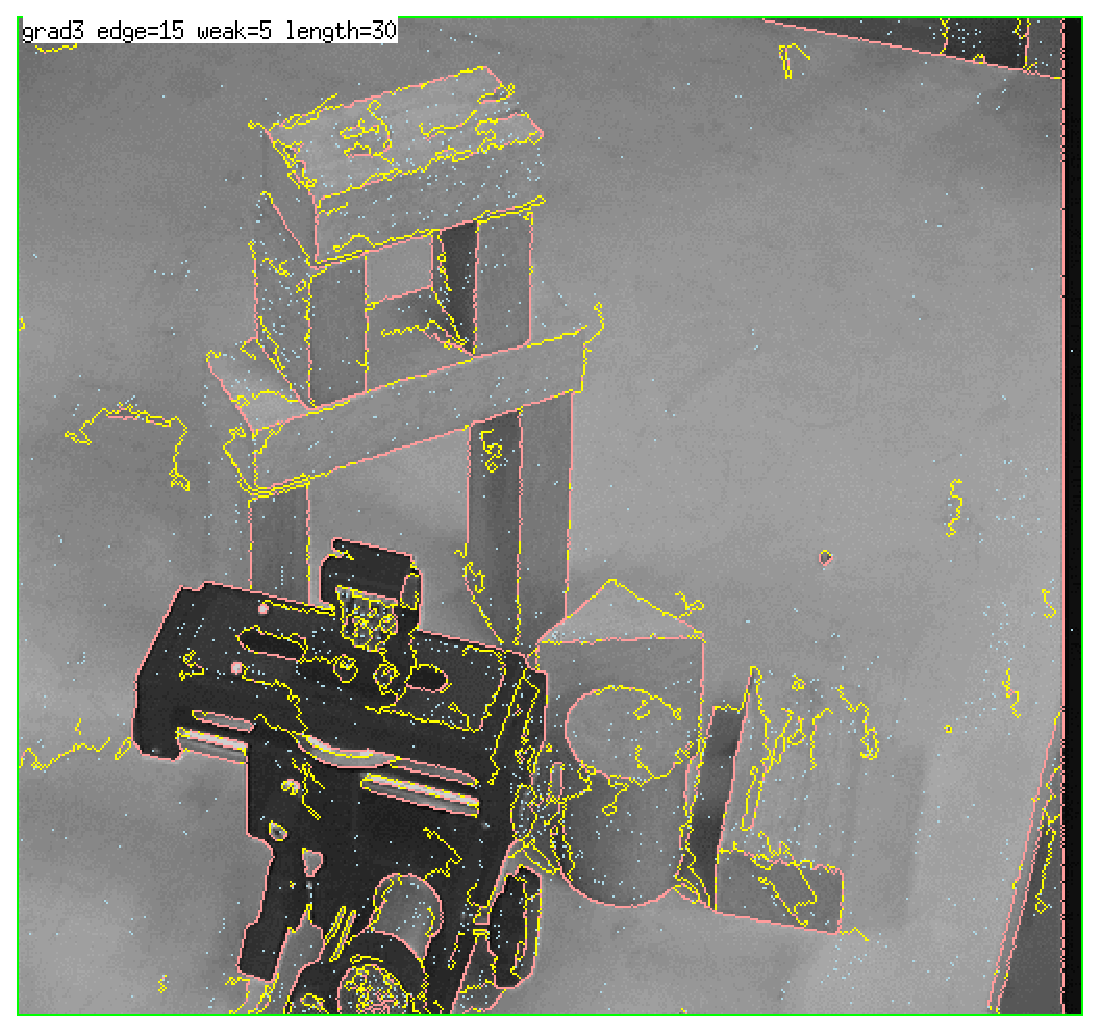
\includegraphics[height=9cm]{fig/block1.edg.ps}
%\epsfile{file=fig/block1.edg.ps,height=9cm}
\caption{Edge Finder and Overlaied Edges}
\end{center}
\end{figure}

\subsection{\label{tracking}トラッキング}
{\tt "vision/correlation"}に元画像とトラッキングしたい画像との
相関を求める関数が定義されている。

\begin{refdesc}
\classdesc{tracking-window}{pixel-image}{x-pos y-pos x-vel y-vel\\
\>pattern-size window-size\\
\>x-win y-win window window-margin\\
\>update threshold half-pattern correlation}{
このクラスは、トラッキング画像を定義する。}

\methoddesc{:correlation}{}{
この画像と元画像との間の相関を返す。}
\methoddesc{:grab}{\&optional (x x-pos) (y y-pos) (sampling 2)}{
画像入力装置から画像を取り込み、その画像の{\bf pixel-image}を返す。}
\methoddesc{:window-rectangle}{val}{
Xwindowの上に四角形を描く。}
\methoddesc{:rectangle}{val}{
Xwindowの上に四角形を描く。}
\methoddesc{:move}{newpos \&aux (newx (aref newpos 0)) (newy (aref newpos 1))}{
トラッキングする位置を{\em newpos}に移動し、新しい画像を取り込む。}
\methoddesc{:track}{display-window \&optional th}{
Xwindowの画像からこの画像をトラッキングする。}
\methoddesc{:serach}{display-window \&optional th}{
Xwindowの画像からこの画像を捜す。}
\methoddesc{:track-and-search}{flag \&optional th}{
この画像をトラッキングする。
もし、トラッキングを失敗したとき、Xwindowからこの画像を捜して
位置を更新する。}

\methoddesc{:pos}{}{
windowの左上位置を返す。}
\methoddesc{:vel}{}{
トラッキング速度を返す。}
\methoddesc{:insidep}{pos \&aux (x (aref pos 0)) (y (aref pos 1))}{
{\em pos}が{\bf tracking-window}の中に含まれるかどうかをチェックする。}
\methoddesc{:update}{\&optional (flag :get)}{
{\tt update}に{\em flag}を設定する。もし、{\em flag}がなければ、
{\tt update}を返す。}
\methoddesc{:prin1}{strm \&rest mesg}{
この{\bf tracking-window}を名前と次元と一緒に表示する。}
\methoddesc{:init}{x y size win-size}{
{\bf tracking-window}を作成する}
\end{refdesc}

\subsection{\label{PBMfile}画像ファイル入出力}
%There are lots of file formats defined for the representation of
%pixel images.
{\tt "vision/pbmfile"}は、Euslispとディスクファイルとの間の
画像データを変換する関数を定義している。
EusLispは、pgm(portable gray-scale map)とppm(portable pixmap)フォーマット
のファイルの読み書きができる。

\begin{refdesc}
\funcdesc{read-pnm}{f \&optional buf0 buf1 buf2}{
{\bf file-stream}の{\em f}で指定されるpgmあるいはppmファイル
を読み込み、{\bf pixel-image}あるいは{\bf color-pixel-image}を返す。
画像ファイルは、asciiでもバイナリーでも可能である。
言い換えれば、P2,P3,P5,P6フォーマットは認識できる。}
\funcdesc{read-pnm-file}{file \&optional buf0 buf1 buf2}{
ファイル名{\em file}で指定されるpgmあるいはppmファイルを読み込む。
%この関数は、{\bf read-ppm}を呼び出す。
}

\funcdesc{write-pgm}{f image  \&optional (depth 255)}{
{\em image}で指定される{\bf pixel-image}を{\bf file-stream}である{\em f}
にバイナリーppmフォーマットで書き込む。
%(この関数は、コメントを追加することで変更できる。)
}
\funcdesc{write-ppm}{f image  \&optional (depth 255)}{
{\em image}で指定される{\bf pixel-image}を{\bf file-stream}である{\em f}
にバイナリーpgmフォーマットで書き込む。}
\funcdesc{write-pnm}{f img}{
{\em img}で指定されるピクセル画像を{\bf file-stream}である{\em f}に書き込む。
もし、{\em img}が{\bf pixel-image}であるなら、バイナリーpgmフォーマットで
書き込み、{\bf color-pixel-image}ならバイナリーppmフォーマットで書き込む。}
\funcdesc{write-pnm-file}{file img}{
ファイル名{\em file}に{\em img}で指定されるピクセル画像を書き込む。
この関数は、{\bf write-pnm}を呼び出す。}

\funcdesc{image::read-raw-image}{file \&optional (x 256) (y x)}{
raw-imageファイルを読み込み、1次元の文字列ベクトルを返す。
%座標系についてなにも前提がない。
raw-imageの次元は、与えられた{\em x}と{\em y}に一致しなければならない。}
\funcdesc{image::write-raw-image}{file imgvec}{
ピクセル値を1バイトのベクトル(文字列)に蓄積した{\em imgvec}を{\em file}
に書き込む。}
\end{refdesc}

\newpage

\section{\label{ManipulatorModel}マニピュレータ}
\markright{\arabic{section}. マニピュレータ}
\hfill {\em documented by Hiromu Onda}

{\bf rotational-joint}クラスと{\bf manipulator}クラスのインスタンスからマニピュレータ
モデルは構成される。{\bf rotational-join}クラスは、{\bf body}のサブクラスであり、
マニピュレータの間接モデルを定義する。
{\bf manipulator}は、{\bf cascaded-coords}のサブクラスであり、運動方程式と逆運動方程式の
解を求めるメソッドを持っている。

マニピュレータを定義するには、
すべての関節を作成した後、{\bf manipulator}にそれらを統合する。

\subsection{
%\label{JointModel}
関節のモデル}

クラス{\bf rotational-joint}が関節のモデルを記述する。
クラス{\bf rotational-joint}は、{\bf body}をスーパクラスに持ち、
その形状モデル、座標系に加えて
関節回転軸、回転角度、可動角度範囲、などを管理している。
次の{\bf defjoint}マクロによって{\bf rotational-joint}
のインスタンスが作成され、{\em joint-name}にバインドされる。
{\bf parent}には、親の関節を指定する。
ベースと指には可動軸を指定する必要はない。

\begin{refdesc}
\longdescription{defjoint}{joint-name \&key \= :shape \hspace{10mm}\= {\it body-object} \` [マクロ]\\
% \hspace{70mm} [マクロ]\\
\> :color \> {\it color-id} \hspace{2cm} \= ;0-15 for MMD \\
\> :parent \> {\it parent-joint} \\
\> :axis \> {\it rotational-axis} \>  ; :x, :y or :z \\
\> :offset \> {\it trans-from-parent-joint} \\
\> :low-limit \> {\it joint-angle-limit-low} \\
\> :high-limit \> {\it joint-angle-limit-hight}}{
関節のモデルを記述する。}
\end{refdesc}

\subsection{
%\label{MultiJointsManipulator}
多関節マニピュレータ}

マニピュレータモデルはクラス{\bf manipulator}によって記述される。
マニピュレータモデルを作成するには、
次の{\bf defmanipulator}マクロを用いる。

\begin{refdesc}
\longdescription{defmanipulator}{manipulator-name \&key \= :class \hspace{2cm} \= {\it manipulator-class} \` [マクロ]\\
%manipulator-class} \hspace{25mm} [マクロ]\\
\> :base \> {\it base-joint} \\
\> :joints \>  {\it list-of-all-joints} \\
\> :hand \> {\it handjoint} \\
\> :left-finger \> {\it left-finger}\\
\> :right-finger \> {\it right-finger}\\
\> :handcoords \> {\it trans-from-hand-to-armsolcoords}\\
\> :toolcoords \> {\it trans-from-armsolcoords-to-toolcoords} \\
\> :open-direction \> {\it finger-open-direction}\\
\> :right-handed  \> {\it righty-or-lefty}}{
マニピュレータモデルを作成する。}

\classdesc{rotational-joint}{body}{(axis offset high-limit low-limit)}
{6自由度マニピュレータの間接を記述する。}

\classdesc{manipulator}{cascaded-coords}{(base baseinverse joint angles right-handed hand handcoords\\
\> right-finger left-finger openvec max-span\\
\> toolcoords toolinverse armsolcoords toolinverse armsocoords\\
\> approach grasp affix)}
{ベースからハンドまでのマニピュレータの運動を管理する。}

\methoddesc{:newcoords}{newrot \&optional newpos}{ 
関節角度が限度に収まっていれば座標系を
{\em newrot}と{\em newpos}に更新する 
}
\methoddesc{:armsolcoords }{}{
ベース座標系からハンド座標系への変換(座標系のインスタンス)を計算し、作成する。
%  ベースからハンドに至る変換を求める
}
\methoddesc{:tool}{\&rest msg}{
 工具座標系を返す、または変更する
}
\methoddesc{:set-tool}{newtool \&optional offset copy}{
 工具座標系{\tt toolcoords}に{\em newtool}を設定する
}
\methoddesc{:reset-tool }{}{
 工具座標系を初期値に戻す
}
\methoddesc{:worldcoords }{}{
 工具座標系の位置ベクトル、回転行列、座標系のワールド表現を求める
}
\methoddesc{:set-coords }{}{
順運動の解を求めるために、座標系を強制的に設定する。
% 一旦順キネマを計算し、そこからさらに各関節角度を求める
}
\methoddesc{:config }{\&optional (a newangles)}{
 6つの関節角度を直接に設定する
}
\methoddesc{:park }{}{
 初期姿勢に戻す
}
\methoddesc{:hand}{\&optional (h nil)}{
 ハンドオブジェクトを返す
}
\methoddesc{:handcoords}{}{
 ハンド座標系の位置ベクトル、回転行列、座標系のワールド表現を求める
}
\methoddesc{:span}{}{
 現在の指の間隔を返す
}
\methoddesc{:open-fingers}{s \&optional abs \&aux (current (send self :span))}
{
 指幅を相対的、絶対的に指定する
}
\methoddesc{:close-fingers}{}{
 指を完全に閉じる 
}
\methoddesc{:angles}{\&optional flag}{
 現在の姿勢の関節角度のリストを返す
}

% \methoddesc{:right-handed}{}{
%% ソースそのものがありませんでした。
% 右手姿勢、左手姿勢を選択する
%}

\methoddesc{:get-approach }{}{
 現在アプローチしている対象を返す
}
\methoddesc{:set-approach }{a}{
 アプローチ対象{\it a}を設定する
}
%\methoddesc{:get-grasp}{}{
%(:get-grasp () grasp-config)
%??? 
% 把握姿勢にある対象物を返す
%}
\methoddesc{:set-grasp}{g}{
 把握対象物{\it g}を指定する
}
\methoddesc{:get-affix}{}{
 把握している物体を返す
}
\methoddesc{:affix}{\&optional (grasp)}{
{\bf affixed-object}に{\tt grasp}を設定する。
{\tt grasp}は、子孫として{\tt handcoords}に関連付けられる。
% 把握を指示する
}
\methoddesc{:unfix}{\&optional (margin 10.0)}{
{\bf affixed-object}にNILを設定する。
{\tt grasp}は、{\tt handcoords}の子孫リストから外される。
% 把握物体を解放したことを指示する
}
\longdescription{:create}{\= \&rest args \` [メソッド]\\
%\longdescription{:create}{\= \&rest args \hspace{111mm} [メソッド]\\
\> \&key \= (:name nm) (:hand h) (:joints j)\\
\> \> (:left-finger lf) (:right-finger rf)\\
\> \> ((:toolcoords tc) (make-coords))\\
\> \> ((:handcoords hc) (make-coords))\\
\> \> ((:base bs) (make-cascoords))\\
\> \> (open-direction (floatvector 0 1 0))\\
\> \> ((:max-span mspan) 100.0)\\
\> \> ((:lefty lft) t)\\
\> \> ((:act a) nil)\\
\> \&allow-other-keys}{
新しいマニピュレータオブジェクトを作成、初期化する
}
\end{refdesc}

{\bf manipulator}オブジェクトは、
{\bf base、joints(J1\ldots J6)、handcoords、toolcoords}
の座標系の繋がりを管理する。
%図\ref{ManipulatorObject}に{\bf manipulator}オブジェクトのスロット構成を、
%表\ref{ManipulatorMethods}に受け付けられるメソッドを掲げる。
{\bf manipulator}クラスは、{\bf cascaded-coords}のサブクラスであり、
やはり、{\bf cascaded-coords}(または{\bf body}などのサブクラス)
である{\bf base}に結合され、
{\bf base}から{\bf toolcoords}(手先座標系)への変換を管理している。
したがって、{\bf manipulator}オブジェクトに対して送られる
{\bf :translate、:locate、:rotate、:orient、:transform}
などのメッセージは、手先点に対して作用する。
そのとき同時にWRTパラメータを指定すれば、
手先はWRT座標系に対して動く。
次のプログラムでは、{\bf eta3}を{\bf manipulator}のインスタンスと仮定している。

\begin{verbatim}
 (send eta3 :translate #f(0 0 -100))        ;手先を10cm引っ込める 
 (send eta3 :translate #f(0 0 -100) :world) ;10cm下げる
 (send eta3 :translate #f(0 0 -100)
             (manipulator-base eta3))     ;手先をベース座標系で10cm下げる
\end{verbatim}

これらのメッセージに対して、manipulatorはアーム解を計算して6つの
関節角度を決定する。
一般に解は複数存在するが、{\bf right-handed}(右手系、左手系)
の区別、および現在の関節角度との連続性により適当な解が選択される。
しかし、指定された位置、姿勢に対する解が存在しない場合や関節角が
限界を越える場合は移動、回転は起こらず、警告が発せられる。

アーム解の計算は、実際のマニピュレータに対応した
個々のmanipulatorクラスに定義された{\bf :armsol}メソッドが行う。
マニピュレータがワールド座標系のどこに置かれてもよいように、
また、どのような工具を用いてもよいように、アーム解は、
{\bf base、toolcoords}とは独立に、base座標系中でのハンドの位置、姿勢に
対して与えられる。

{\bf base、J1、J2、\ldots 、handcoords、toolcoords}の関係を図\ref{JointCoords}
に示す。
ワールドから手先への変換を$T$とすると、$T$および各部分変換は次のようにし
て得られる。

$
\begin{array}{ll}
T & = base \cdot J1 \cdot J2 \cdot \ldots 
\cdot J6 \cdot handcoords \cdot toolcoords \\ 
 & = (send \; eta3 \; :worldcoords) \\ 
T_{Jn} & = base \cdot J1\cdot \ldots \cdot Jn \\
 & = (send \; Jn \; :worldcoords) \\
T_{arm} & = J1 \cdot J2 \cdot \ldots \cdot J6 \cdot handcoords \\ 
 & = (send \; eta3 \; :armsol-coords) \\ 
T_{tool} & = J1 \cdot J2 \cdot  \ldots \cdot J6 \cdot handcoords \cdot toolcoords \\ 
 & = (send \; eta3 \; :copy-coords) \\
T_{t} & = toolcoords \\ 
 & = (manipulator-toolcoords \; eta3)\\
T_{t}^{-1} & = toolcoords^{-1} \\ 
 & = (manipulator-toolinverse \; eta3) \\
T_{h} & = handcoords \\ 
 & = (manipulator-handcoords \; eta3)\\
\end{array}$

ここで、$T$はワールド座標系から工具座標系まで変換する。

\begin{figure}
\begin{center}
%%% change 2004.12.14 \epsfile{file=/usr/share/src/eus/doc/latex/fig/eta3coords.ps,height=100mm}
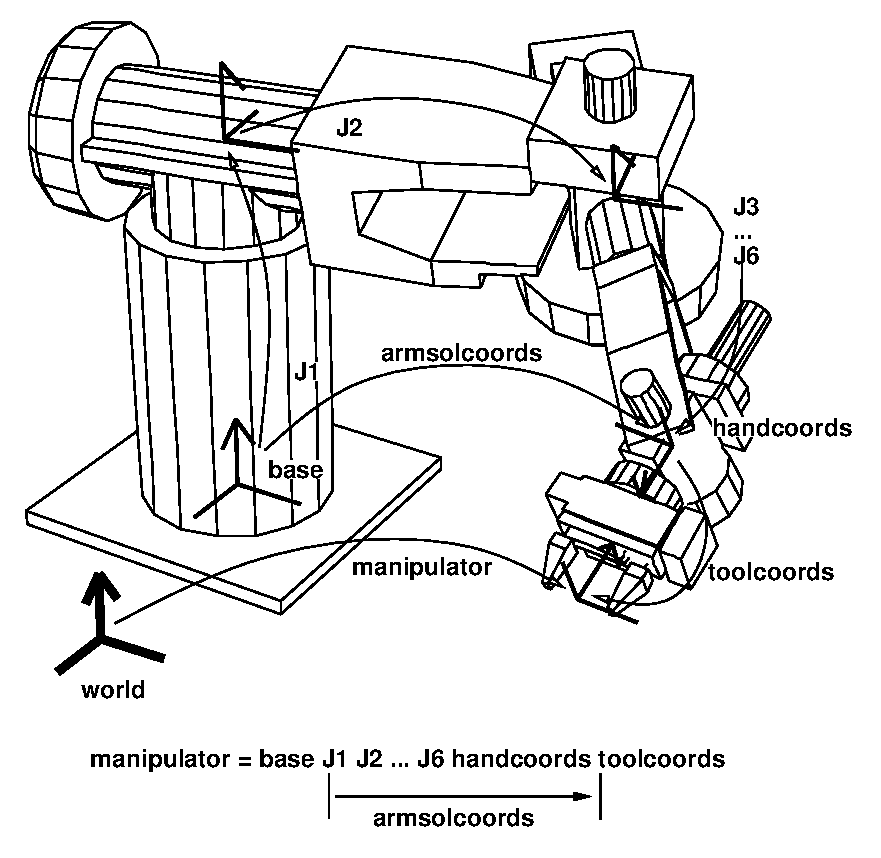
\includegraphics[height=100mm]{fig/eta3coords.ps}
%\epsfile{file=fig/eta3coords.ps,height=100mm}
\end{center}
\caption{\label{JointCoords}
relation between coordinate systems in a manipulator}

\end{figure}


各関節は、Brepで表現された幾何モデルを保持している。しかし、頂点の座標、
平面の方程式は常に現状を反映しているとは限らない。マニピュレータに対する
移動、回転などのメッセージでは座標系の更新だけを行い、頂点の座標は変化し
ない。これは、移動、回転が複数回続けて起こった場合の計算量を減らすためで
ある。更新は、マニピュレータに{\bf :worldcoords}メッセージを送る
ことで引き起こされる。


マニピュレータは、手先座標系で動作を指定することを主な目的としている。
関節角による指定には {\bf :config} を用いる。
引き数には6要素の列を与える。

\begin{verbatim}
  (send eta3 :config (float-vector pi/2 pi/2 0 1 0 1))
\end{verbatim}

{\bf :config}は、各関節角度が可動範囲に収まっていることを検査した後、
それらを回転させる。
この結果、マニピュレータの管理している座標系と
関節角度から定まる実際の手先の位置姿勢とが一致しなくなる。
両者を一致させるためには、{\bf :set-coords}メッセージを送る。
{\bf :set-coords}は、関節角度から順方向のキネマティクスを計算し、
最終的な手先座標系に対してさらにアーム解を解く。


例 ETA3のモデル生成とその描画
\begin{verbatim}
EusLisp 7.27 with Xlib created on Thu Sep 17 14:33:30 1992
(load "view.l")                                ;ウィンドウを開く
(load "/usr/local/eus/robot/eta3/eta3build.l") ;ETA3のモデルを生成する
(send *viewing* :look #f(2000 2000 2000))      ;視点を変える
(send-all (eta3arm-components eta3) :color 1)  ;物体の線の色を黒に変える
(send eta3 :config (float-vector 0 (/ -Pi 4.0) Pi/2 0 (/ -Pi 4.0) 0 ))
					       ;ETA3を関節角度の指定で動かす
(send eta3 :set-coords)                        ;上記参照
(draw eta3)                                    ;ETA3を描画する
\end{verbatim}

\newpage

\newpage

\section{\label{MARS} MARS: マルチ自律ロボットシミュレータ}
\markright{\arabic{section}. MARS}
\hfill {\Large \em (予告)}

\hfill {\em 著者: 国吉 康夫,電総研}

{\bf MARS}は、平面空間内における
マルチ自律移動ロボットのためのシミュレーション環境である。
このプログラムは、Euslispで記述されている。

{\bf 開発状況:}
1995年1月、MARSの発表直前バージョンが電総研内で用いられている。
システムの改善を活発に行い、1995年の上期内に最初のバージョンを
発表する計画である。
その後も、システムの向上をはかり、1996年3月までに安定した状態を
達成したいと望んでいる。
発表の告示はEuslispのメーリングリストや他のインターネットサービス
を通じて行われる予定である。
恐らくライセンスの条件をEuslispから分けるであろう。

{\bf 目的:}
MARSは、単一あるいは複数の移動ロボットで知的ロボットの研究に使用することを
意図してつくられている。たとえば、行動学習やマップ構築や知能収集や
複数ロボット協調や協調学習などである。


\subsection{始め方}
MARSプログラムは、{\bf robot/MARS/ver.XXX}にある。
最初に、".eusrc"ファイルを自分のホームディレクトリにコピーする。
必要があれば変更すること。
(MARSがインストールされているディレクトリのパス名など)

このディレクトリから{\bf eusx}を呼び出す。
すべてのファイルが自動的にロードされ、シミュレータが動作し始める。
windowがオープンされ、初期メッセージが下部windowに現れるまで待つこと。

例:
\begin{verbatim}
Try "SYSTEM"->"Load" menu.
Load "example.bbs".
And "SCL"->"On" menu.
\end{verbatim}

注意:\\
SCL$\rightarrow$"Off" シミュレーションは一時停止するが、GUI処理は続行される。\\
SYSTEM$\rightarrow$"Quit" 最上位のループから抜ける。(mars-loop)により再開できる。\\
SYSTEM$\rightarrow$"Save" 現在の状態をファイルにセーブする。\\
SYSTEM$\rightarrow$"All-Clear" すべてを消し、システムを初期化する。\\
SYSTEM$\rightarrow$"Reset" ロボットの内部状態をリセットするために使用する(特殊目的)。\\

\subsection{システム概要}

\begin{figure}[h]
\begin{center}
%\begin{tabular}{c@\extracolsep{1em}c}
\begin{tabular}{c c}
%%% change 2004.12.14 \epsfile{file=fig/mars.eps,scale=0.3} & % I=;f$HF1$83($KJQ99$7$F!#
%%% change 2004.12.14 \epsfile{file=fig/simst.ps,hscale=0.42,vscale=0.45} \\
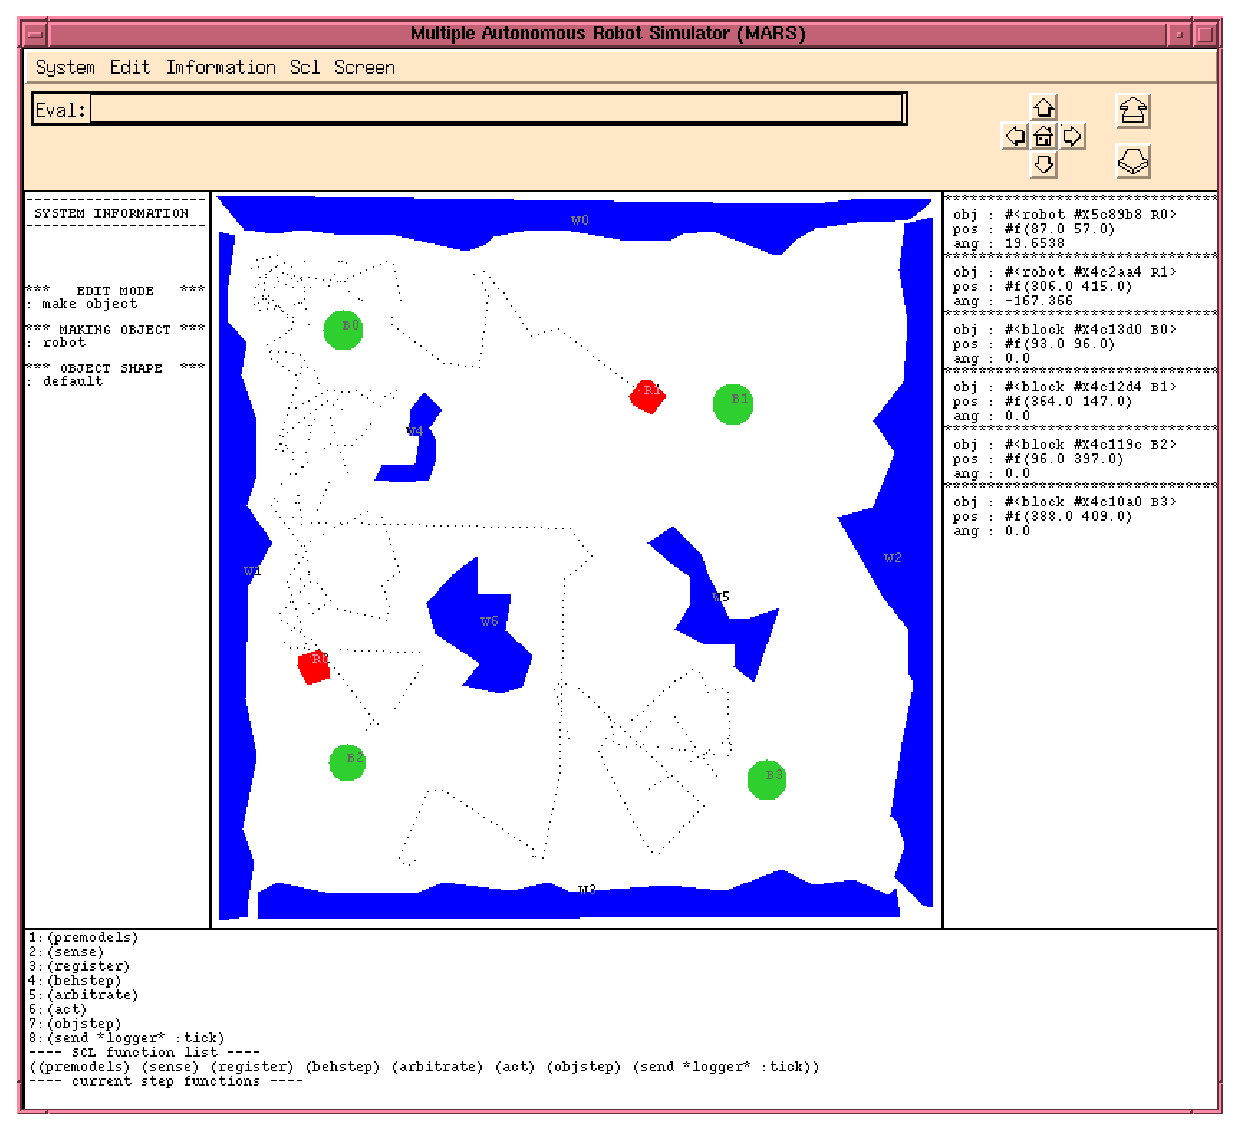
\includegraphics[width=0.4\columnwidth]{fig/mars.eps} &
%\epsfile{file=fig/mars.eps,width=0.4\columnwidth} & % I=;f$HF1$83($KJQ99$7$F!#
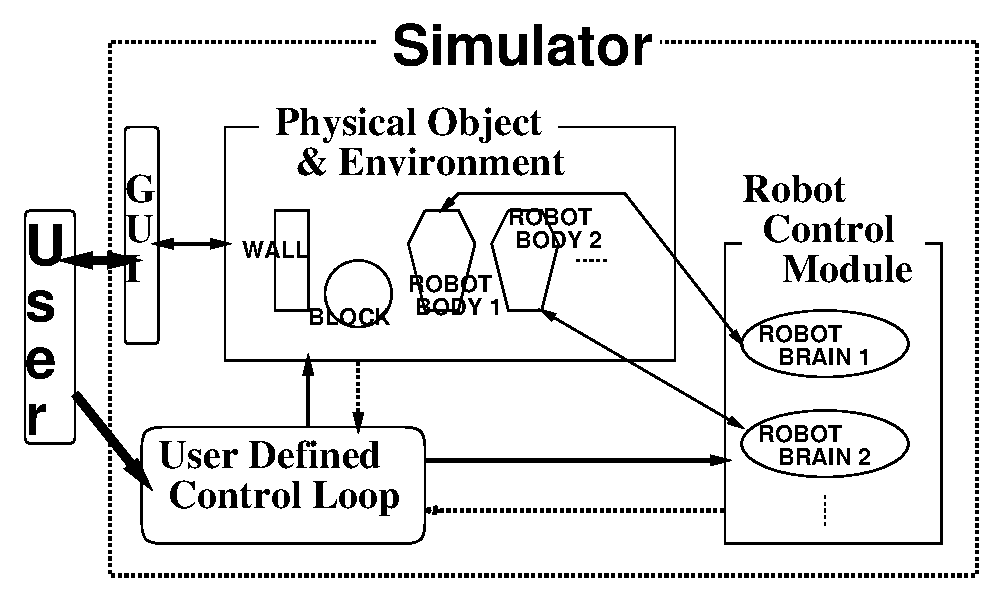
\includegraphics[width=0.6\columnwidth]{fig/simst.ps} \\
%\epsfile{file=fig/simst.ps,width=0.6\columnwidth} \\
\end{tabular}
\caption{\label{MARSOverview} MARS windowの表示例(左)と
プログラムの構造(右)}
\end{center}
\end{figure}

MARSを始めたとき、図~\ref{MARSOverview}(左)に示されるような
メインwindowを見ることができる。MARSは、図~\ref{MARSOverview}(右)
のようなモジュールアーキテクチャを採用している。
それは、物理シミュレーションモジュールとロボット制御モジュールと
ユーザーインターフェースモジュールとユーザーが定義したグローバル
制御ループにより構成されている。

{\bf 物理シミュレーション:}
現在の物理シミュレーションモジュールは、4つのタイプのオブジェクトを
処理している。
{\bf wall} (固定障害物), {\bf block} (移動障害物), {\bf
robot-body} (活動オブジェクト)と{\bf magic-block} (経験学習するための
特別な報酬を与えるオブジェクト)である。

\begin{figure}
\begin{center}
%\begin{tabular}{c@\extracolsep{1em}c}
\begin{tabular}{c c}
%%% change 2004.12.14 \epsfile{file=fig/robot-ui2.ps,hscale=0.5,vscale=0.5} &
%%% change 2004.12.14 \epsfile{file=fig/robot-st2.ps,scale=0.4} \\
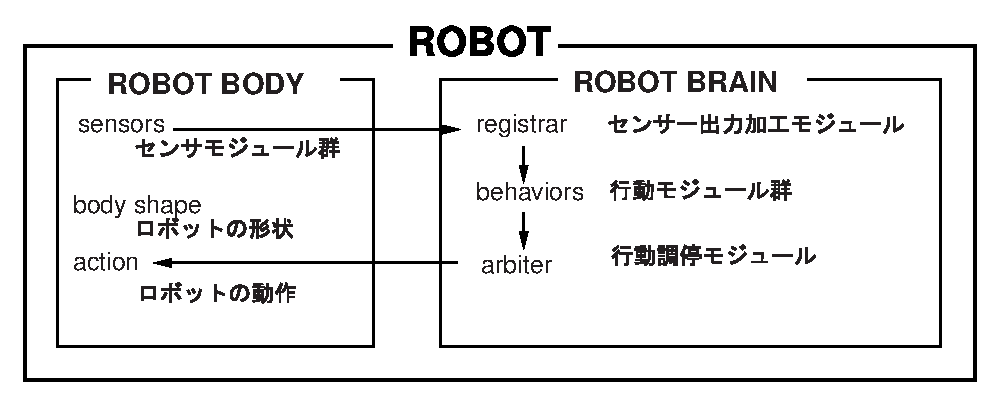
\includegraphics[width=0.5\columnwidth]{fig/robot-ui2.ps} &
%\epsfile{file=fig/robot-ui2.ps,width=0.5\columnwidth} &
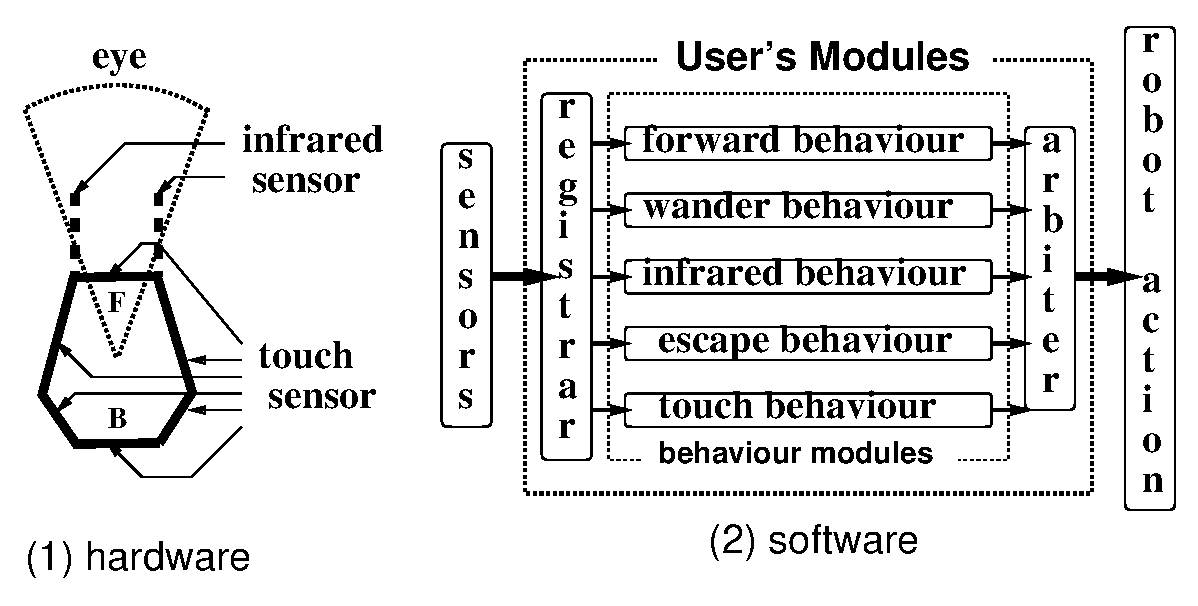
\includegraphics[width=0.5\columnwidth]{fig/robot-st2.ps} \\
%\epsfile{file=fig/robot-st2.ps,width=0.5\columnwidth} \\
\end{tabular}
\end{center}
\caption{\label{fig:robotst}ロボットの内部構造(左)と
ビヘービアベーストロボットの構成例(右)}
\end{figure}

{\bf ロボットモデル:}
物理的シミュレーションモジュールとロボット制御モジュールとの
間のインターフェースである。
いくつもの{\bf robot}モデルを生成することができ、
擬似並列でシミュレートできる。
{\bf robot}はそれぞれ、{\bf robot-body}と{\bf robot-brain}の
のモジュールの組みで構成される。
{\bf robot-body}は、ロボットの物理的な性質を定義し、
{\bf robot-brain}はロボットの行動を定義する。

{\bf センサモデル:}
ユーザーは、{\bf robot-body}のどこにでもいくつものセンサを
選択して取り付けることができる。
現在、実現されているセンサモデルは、以下のものである。
{\bf 距離センサ} (走行距離), {\bf 角度センサ} (回転角),
{\bf 接触センサ}, {\bf 赤外線センサ}, {\bf レーザセンサ} (超音波), 
{\bf 視覚センサ} (object-name-sensor)。
現在のバージョンでは、ノイズや不確定要素について考えていない。

{\bf ロボット知能:}
{\bf robot-brain}は、シミュレートしたセンサデータを処理したり
行動命令を生成するためにユーザーで定義されたモジュールである。
センサデータを受け、行動命令を出力しなければならない。
付け加えて、リエントラントプログラムとして書かれていて、
グローバル制御ループによって送られる{\bf :step}メッセージ
によって時間分割されなければならない。
これらの拘束に合う限り、ユーザーはどんな認識アーキテクチャも
採用することができる。
システムは、デフォルトとしてビヘービアベースト型のアーキテクチャ
の例を備えている。

{\bf GUI:}
{\bf MARS}のメインwindowは、システムを制御するためにいくつかのボタンを
持つメニューバーを持っている。
また、システムは物理環境を生成/変更するための内部グラフィックエディタ
を持っている。
ファイルに対してエージェント定義と一緒に物理環境を読み書きできる。

{\bf ネットワーク拡張:}
{\bf robot-brain}は、非同期ソケット通信を通して外部プロセス
との接続を構築することができる。
この場合、ユーザーは{\bf remote-brain}を記述するために任意の言語(C,
Prolog, Scheme, Perl, etc...)を使用することができる。
非同期接続のおかげで、ユーザーは時間分割について少しも気にする必要が無い。

{\bf 経験学習機能:}
{\bf MARS}は、ロボットが経験学習するための幾つかの特殊機能を備えている。
報酬を与えるオブジェクトや報酬センサ(報酬値をロボットに送るもの)
や報酬ログ(システム全体の報酬の統計を計算するもの)である。

%
\cleardoublepage
\markboth{Euslisp version \eusversion リファレンスマニュアル}{Index}
\footnotesize
\printindex
\end{document}

